%% This is file `elsarticle-template-1-num.tex',
%%
%% Copyright 2009 Elsevier Ltd
%%
%% This file is part of the 'Elsarticle Bundle'.
%% ---------------------------------------------
%%
%% It may be distributed under the conditions of the LaTeX Project Public
%% License, either version 1.2 of this license or (at your option) any
%% later version.  The latest version of this license is in
%%    http://www.latex-project.org/lppl.txt
%% and version 1.2 or later is part of all distributions of LaTeX
%% version 1999/12/01 or later.
%%
%% Template article for Elsevier's document class `elsarticle'
%% with numbered style bibliographic references
%%
%% $Id: elsarticle-template-1-num.tex 149 2009-10-08 05:01:15Z rishi $
%% $URL: http://lenova.river-valley.com/svn/elsbst/trunk/elsarticle-template-1-num.tex $
%%
\documentclass[review,12pt]{cmuthesis}
\usepackage{times}
\usepackage{fullpage}
\usepackage{graphicx}
\usepackage{amsmath}
\usepackage[numbers,sort]{natbib}
\usepackage[backref,pageanchor=true,plainpages=false, pdfpagelabels, bookmarks,bookmarksnumbered,
%pdfborder=0 0 0,  %removes outlines around hyper links in online display
]{hyperref}

% Approximately 1" margins, more space on binding side
%\usepackage[letterpaper,twoside,vscale=.8,hscale=.75,nomarginpar]{geometry}
%for general printing (not binding)
\usepackage[letterpaper,twoside,vscale=.8,hscale=.75,nomarginpar,hmarginratio=1:1]{geometry}

%% Use the option review to obtain double line spacing
%% \documentclass[preprint,review,12pt]{elsarticle}

%% Use the options 1p,twocolumn; 3p; 3p,twocolumn; 5p; or 5p,twocolumn
%% for a journal layout:
%% \documentclass[final,1p,times]{elsarticle}
%% \documentclass[final,1p,times,twocolumn]{elsarticle}
%% \documentclass[final,3p,times]{elsarticle}
%% \documentclass[final,3p,times,twocolumn]{elsarticle}
%% \documentclass[final,5p,times]{elsarticle}
%% \documentclass[final,5p,times,twocolumn]{elsarticle}

%% The graphicx package provides the includegraphics command.
\usepackage{graphicx}
%% The amssymb package provides various useful mathematical symbols
\usepackage{amssymb}
%% The amsthm package provides extended theorem environments
%% \usepackage{amsthm}

%% The lineno packages adds line numbers. Start line numbering with
%% \begin{linenumbers}, end it with \end{linenumbers}. Or switch it on
%% for the whole article with \linenumbers after \end{frontmatter}.
\usepackage{lineno}

% Set the typeface to Times Roman
\usepackage{times}

\usepackage{hyperref}
\usepackage{url}
\usepackage{natbib}
\setcitestyle{authoryear,round,citesep={;},aysep={,},yysep={;}}
\usepackage{epsfig}
\usepackage{microtype}
\usepackage{amsmath}
\usepackage{amssymb}
\usepackage{amsthm}

\usepackage{bbold}
\usepackage{flushend}
\usepackage{subfig}
\usepackage{array}
\usepackage{comment}
\usepackage{subfig}
\usepackage{longtable}
\usepackage{hhline}
\usepackage{helvet}
\usepackage{courier}

\usepackage[final]{pdfpages}

\usepackage{enumitem}

%\usepackage[ruled,vlined,linesnumbered,resetcount]{algorithm2e}

\usepackage{booktabs}       % professional-quality tables
\usepackage{amsfonts}       % blackboard math symbols
%\usepackage{nicefrac}       % compact symbols for 1/2, etc.
\usepackage{microtype}      % microtypography
\usepackage{algorithm}
\usepackage{algorithmic}

\usepackage{caption}
%\usepackage{subcaption}
\usepackage{xspace}
\usepackage{color}

\usepackage{amsthm}

\usepackage{bbm}
\usepackage{multirow}



%\newtheorem{theorem}{Theorem}[section]
%\newtheorem{lemma}[theorem]{Lemma}
%
%\theoremstyle{definition}
%\newtheorem{definition}[theorem]{Definition}
%\newtheorem{example}[theorem]{Example}
%\newtheorem{xca}[theorem]{Exercise}

%\theoremstyle{remark}
%\newtheorem{remark}[theorem]{Remark}

\newcommand{\E}{\mathbb{E}}
\newcommand{\R}{\mathbb{R}}
\newcommand{\angleb}[1]{\langle #1 \rangle}

\newcommand{\at}[1]{\langle #1 \rangle}
\newcommand{\XX}{\textbf{X}}
\newcommand{\YY}{\textbf{Y}}


\makeatletter
\newtheorem*{rep@theorem}{\rep@title}
\newcommand{\newreptheorem}[2]{%
\newenvironment{rep#1}[1]{%
 \def\rep@title{#2 \ref{##1}}%
 \begin{rep@theorem}}%
 {\end{rep@theorem}}}
\makeatother

\newcommand{\defmu}{}
\newcommand{\innerprod}[3][\defmu]{{\left\langle {#2},{#3} \right\rangle}_{#1}}
\newcommand{\norm}[2][\defmu]{{\left\lVert {#2} \right\rVert}_{#1}}
\newcommand{\functional}[3][\defmu]{{\mathcal{#2}}_{#1} [#3]}
\newcommand{\risk}[2][\defmu]{\functional[#1]{R}{#2}}

\newreptheorem{theorem}{Theorem}
\newreptheorem{definition}{Definition}


\newtheorem{theorem}{Theorem}[section]
\newtheorem{lemma}[theorem]{Lemma}
\newtheorem{proposition}[theorem]{Proposition}
\newtheorem{corollary}[theorem]{Corollary}
\newtheorem{definition}[theorem]{Definition}
\newtheorem{assumption}[theorem]{Assumption}
\newenvironment{myproof}[1][\proofname]{\proof[#1]\mbox{}}{\endproof}
 
\newcommand{\algname}{Streaming Gradient Boosting\xspace}
\newcommand{\algshort}{SGB\xspace}
\newcommand{\algnospace}{SGB} 





\setcounter{secnumdepth}{5}


\newcommand{\fix}{\marginpar{FIX}}
\newcommand{\new}{\marginpar{NEW}}
\newcommand{\YahooDataset}{Yahoo! Learning to Rank Challenge dataset}
\newcommand{\YahooLTR}{\textsc{Yahoo!\,LTR}}
\newcommand{\GrainDataset}{Agricultural dataset}
\newcommand{\Grain}{\textsc{Agricultural}}


\newcommand{\annnames}{Anytime Neural Networks\xspace}
\newcommand{\annname}{Anytime Neural Network\xspace}
\newcommand{\ann}{ANN\xspace}
\newcommand{\annnp}{ANN} 
\newcommand{\anns}{ANNs\xspace}
\newcommand{\aannnp}{AANN}
\newcommand{\aann}{AANN\xspace}
\newcommand{\aanns}{AANNs\xspace}
\newcommand{\adaloss}{AdaLoss\xspace}
\newcommand{\sieve}{SIEVE\xspace}
\newcommand{\explin}{EXP-LIN\xspace}
\newcommand{\const}{CONST\xspace}
\newcommand{\linear}{LINEAR\xspace}
\newcommand{\round}[1]{\lfloor #1 \rceil}

% petridish
\newcommand{\stopforward}{\textrm{sf}}
\newcommand{\stopgradient}{\textrm{sg}}
\newcommand{\petridishhard}{Isolated\xspace}
\newcommand{\petridishsoft}{Joint\xspace}
\newcommand{\Petridish}{Petridish\xspace}
\newcommand{\PetridishCP}{Petridish-CP\xspace}
\newcommand{\PetridishWS}{Petridish-WS\xspace}

\newcommand{\todo}[1]{\textcolor{red}{#1}}
\newcommand{\dd}[1]{\textcolor{blue}{#1}}


\DeclareMathOperator*{\argmax}{arg\,max} 
\DeclareMathOperator*{\argmin}{arg\,min}

\allowdisplaybreaks



\newcommand{\GOMPDIR}{1_gomp}
\newcommand{\SGBDIR}{2_sgb}
\newcommand{\ANNDIR}{3_ann}
\newcommand{\NASDIR}{4_nas}



%% natbib.sty is loaded by default. However, natbib options can be
%% provided with \biboptions{...} command. Following options are
%% valid:

%%   round  -  round parentheses are used (default)
%%   square -  square brackets are used   [option]
%%   curly  -  curly braces are used      {option}
%%   angle  -  angle brackets are used    <option>
%%   semicolon  -  multiple citations separated by semi-colon
%%   colon  - same as semicolon, an earlier confusion
%%   comma  -  separated by comma
%%   numbers-  selects numerical citations
%%   super  -  numerical citations as superscripts
%%   sort   -  sorts multiple citations according to order in ref. list
%%   sort&compress   -  like sort, but also compresses numerical citations
%%   compress - compresses without sorting
%%
%% \biboptions{comma,round}

% \biboptions{}


\title{
{Anytime Prediction and Learning for \\
the Balance between Computation and Accuracy}\\
}
\author{
Hanzhang Hu}

\date{April, 2019}
\Year{2019}
\trnumber{CMU-ML-19-106}

\committee{
J. Andrew Bagnell (Co-chair)\\
Martial Hebert (Co-chair)\\
Ruslan Salakhutdinov \\
Rich Caruana}

\support{This research was sponsored by the Office of Naval Research award numbers N000140911052 and N000141512365, the US Army Research Laboratory award number W911NF1020016, and a gift from Verizon Media.}


\begin{document}


\maketitle


\chapter*{Abstract}
When choosing machine learning algorithms, one often has to balance between two opposing factors, 
the computational speed and the accuracy of predictors. 
The trade-off during testing is often difficult to balance, 
because the test-time computational budget may be agnostic
at training, and the budget may vary during testing. 
Analogously, given a novel data-set, one often lacks prior knowledge in the appropriate predictor complexity
and training computation, and furthermore, may want to interrupt or prolong the training 
based on training results. 

In this work, we address these trade-offs between computation and accuracy via \emph{anytime} prediction and 
learning, which are algorithms that can be interrupted at any time and still produce valid solutions. 
Furthermore, the quality of the results improves with the consumed computation before interruption. 
With the versatility to adjust to any budget, anytime algorithms automatically
 utilize any agnostic computational budget to the maximum extent.

To address the test-time trade-off, we study anytime predictors, whose prediction computation can be interrupted during testing. 
We start with developing provably near-optimal anytime linear predictors, and derive a theoretical performance limitation
for anytime predictors that are based on ensemble methods. Then we develop practical 
anytime predictions within individual neural networks via multi-objective optimization. 
Furthermore, leveraging these anytime predictors as weak learners, we circumvent the
performance limitation on ensemble-based anytime predictors.

For the train-time trade-off, we consider the neural architecture search problem, where
one seeks the optimal neural network structure for a data-set. We draw a parallel between this bi-level 
combinatorial optimization problem and the feature selection problem for linear prediction, 
and develop an iterative network growth algorithm that is inspired by a forward selection algorithm. 
We also consider the problem of training on large data-sets, and develop 
no-regret gradient boosting algorithms for stochastic data streams.





\chapter*{Acknowledgements} 

I would like to thank J. Andrew Bagnell, Martial Hebert, Ruslan Salakhutdinov, and Rich Caruana, for serving on my thesis committee.
I appreciate them for setting aside time for me, and giving me invaluable discussions and suggestions. 

I am happy to have been working with Drew and Martial for the past years. 
They have given me countless help, despite of their busy schedules. 
They gave me incredible freedom in exploring topics of my choice, 
and were patient with me to allow me gradually formalize and mature the research ideas. 
This experience of research and development has given me many invaluable lessons, and I am grateful to have 
Drew and Martial to guide me through them, like lighthouses in a dark ocean. 

I have been fortunate to have many collaborators over the years, in roughly chronological order,
Daniel Munoz, Alexander Grubb, Allie Del Giorno, Wen Sun, Arun Venkatraman,  Debadeepta Dey, and John Langford. 
They have taught me many things both in research and in life. Without their help, this work would not have
come to be. I especially want to thank Dey for setting up my experiments on his computational resources, 
and he has run thousands of my scripts over the two years. 

\begin{itemize}
\item Chapter~\ref{chapter:anytime_linear} is based on the Ph.D. thesis of Alexander Grubb, who made an 
excellent introduction to gradient boosting and its application to anytime prediction for me. In fact the
main contributions of this chapter are improvements of unpublished results of his thesis.
\item Chapter~\ref{chapter:ann} involves a large number of experiments. Debadeepta Dey kindly offered his 
computational resources in the middle of this project, and without his help on running thousands of
scripts, this work will never come to fruition. 
\item Chapter~\ref{chapter:sgb} came out of a paper reading session of the lab. The careful analysis of 
Wen Sun and the amazing intuition of Drew led to our initial exploration of this topic. We later also extended
previous work of Alexander Grubb on gradient boosting with non-smooth losses to enable streaming gradient 
boosting to do so as well. 
\item Chapter~\ref{chapter:nas} started as an internship project at Microsoft Research under the supervision 
of Debadeepta Dey. Initially this project came out as a bag of engineer hacks that works somehow. 
Thanks to the inputs from John Langford and Rich Caruana, we were able to steer the project into a more 
motivated direction that happens to fit into this thesis nicely.
\end{itemize}

 

\tableofcontents
\listoffigures
\listoftables

\mainmatter


%%
%% Start line numbering here if you want
%%
\linenumbers
\chapter{Introduction}
\label{chapter:thesis_introduction}


When evaluating a predictor for an application, one often needs to consider two critical aspects of algorithms: the accuracy of the prediction, and the computational cost of the predictor. These two factors are often opposed to each other: practitioners typically have the dilemma to choose between predictors that are accurate but slow to compute and ones that are fast but inaccurate. 
This trade-off between computational cost and accuracy is inherently difficult to manage, and is the focus of this work.


\section{Motivations and Problem Settings}

Machine learning algorithms typically have computational budget limits during test-time. For applications on mobile devices and Internet of Things (IoTs), it is critical for the predictors to fit in these devices with low computational power and consume little computation during test-time. For robotic applications such as autonomous vehicle or drones, it is paramount to have low latency in visual detection for planning maneuvers. Web services such as Email spam filters also require low latency to maintain user satisfaction. 
For such applications, one often cannot deploy predictors that achieve the state-of-the-art accuracy, because those predictors often are associated with high computational costs. Instead, these applications often seek the most accurate models that are within their computational budgets. 

Furthermore, the computational budget limits of many applications can also vary during test-time, or can be agnostic during training. 
For instance, robotic applications have varying test-time budget limits based on the speed of the robot and the complexity of the environments. 
Web servers may handle heavier query traffic during the day than during the night, but they are expected to maintain the same low latency. 
Mobile and low-computation devices may want a low-power mode in case of low battery. 
Hence, it is beneficial to consider the setting where we seek the most accurate models at each possible budget limit of the applications. 
We draw special attention to the fact that under this setting, we delay the decision of the budget limits to the test-time, allowing greater flexibility in the algorithms. Furthermore, when the budget limit becomes known, one can extract from the spectrum of cost-efficient models. Alternatively, if one wants to minimize the average test-time computational costs of the prediction given a target accuracy level, such as in budgeted prediction~\ref{cascade_nn,adaptivenn}, one can combine the spectrum of models with early-stopping policies in order to reduce computation on clear decisions and prolong computation on ambiguous ones.

While the above examples and problem settings focus on the balance between model accuracy and test-time computation, practitioners may often be concerned with their train-time computational costs. 
One reason for this concern is that the data-sets are becoming larger and are continuously updated due to improved data storage and collection. Specifically, fields such as finance, information retrieval, computer vision, text and vocal language processing, and etc., each has accumulated data from decades of practice. Training state-of-the-art models against the decades worth of data becomes increasingly challenging. Hence, it is crucial for modern machine learning models to be able to handle large data-sets that may not be present on the same machine or at even the same time. Furthermore, the models ideally should be able to be improved as more data becomes available or more train-time computational resource is allocated. 

Another key reason for the rising train-time computation is the increased model complexity. As neural networks become the dominating methods for 
computer vision tasks and natural language processing, practitioners often rely on experts to find optimal network architectures via trial-and-error. However, such experimental process can be vastly expensive, taking thousands of GPU-days~\citep{nas}, and may yet generalize to general data-sets. Facing such complex and combinatorial hyper-parameter space of model architectures, we need guidance to search in a cost-efficient manner. In particular, practitioners may be interested in increasing the model complexity gradually: one starts with small architectures that can be trained and deployed easily; then as more train-time computation is allowed, the model complexity is gradually increased in a guided manner. Furthermore, ideally one would like the models to reusable and stable, so that new models can utilize previous found models and do not deviate from previous models too much to affect user experience. 

In summary, the targeted problem settings of this work can be partitioned into two parts. The first focuses on the problem of finding accurate predictions at each possible test-time computational budgets, and the second focuses on enabling the previous solutions to handle the rising computational cost in training due to increased data-set sizes and increased complexity in model hyper-parameters. 

\section{Approach}

For each of test-time and train-time trade-off between computation and accuracy, we develop both algorithms with theoretical performance guarantees and algorithms that work well on real-world data-sets. We summarize the main approaches that we take as follows. 

One approach to have accurate predictions at each possible test-time computational budget limit is to first produce crude predictions early, and then continuously improve them. Such algorithms are called \emph{anytime} algorithms, and they automatically adjust to the varying or agnostic test-time budget limits because the algorithm utilize the computational resources until the budget limit. 
One common approach to achieve anytime prediction is through ensembles of weak predictors~\citep{sochman:05,brubaker:07,lefakis:10,reyzin:11,xu:14,cai:15,speedboost}, so that at test-time, one computes the predictors iteratively and then reports the partial ensemble result as the intermediate or anytime results. Indeed, the first anytime predictor of this work follows this idea of combining weak predictors in a generalized linear prediction setting, and utilizes submodular optimization results~\citep{kemp} to bound the performance of the predictions. Furthermore, we prove a limitation of any anytime algorithm that stems from an ensemble of weak predictors, proving that in general such an ensemble of cost $B$ can only achieve comparable rewards of the optimal ensemble of cost $B/4$. 

Such limitations lead us to consider an alternative approach to anytime prediction, where we train a single model to produce multiple intermediate results for anytime predictions, and we optimize all the anytime results jointly. 
Viewing anytime prediction as a multi-objective optimization, we develop an adaptive method to balance the weights of the objectives, and improve anytime prediction quality on multiple neural networks and data-sets. 
By exploiting anytime neural networks as weak learners, we can form ensembles of anytime predictors for anytime prediction, and interestingly, by making weak learners to be anytime predictors, we can circumvent the previous theoretical limitation on ensemble-based anytime predictors.

For the train-time trade-off between computation and accuracy, we specifically target problems that are often accompanied by our anytime predictors. Since anytime models often stem from ensembles of weaker models that are trained sequentially, they can be difficult to scale to large data-sets, especially on data-sets that may be expensive to loop through. To address this weakness, we develop gradient boosting algorithms for stochastic data streams so that we can train all weak learners jointly. Gradient boosting can be considered as approximated gradient descent in the functional space, and can be analyzed via gradient descent~\citep{hazan2007logarithmic,grubb2011generalized}. Combining gradient boosting with analysis from online learning~\citep{beygelzimer2015optimal,cesa2004generalization}, we analyze the proposed algorithms under stochastic data streams. We bound the regrets of the proposed algorithm, showing that it achieves no regret in prediction losses against any competitor under strongly convex losses and under the assumption that each weak online learner can predict better than random by a margin.

We also address the increased complexity of hyper parameters in the specific setting of neural architecture search~\citep{nas,Elsken2018NeuralAS}, where one seeks the optimal architecture given a data-set and an optimization objective. We first formulate the problem as a bi-level optimization and show its connections to the earlier anytime linear prediction problem. 
Inspired by forward selection approach in the linear prediction setting, we propose to expand existing neural networks models iteratively guided by gradient boosting. 
Each step of the model expansion is determined by fitting potential short-cut connections against the gradient of the loss with respect to intermediate layers. 

In summary, the thesis statement of this work is as follows. 
\begin{quotation}
%This work meows a lot but achieves no fish. 
\textbf{Thesis Statement:} 
Modern machine learning applications often have to address the trade-off between computational costs and predictive powers. 
%At test-time, the computational budget is often limited, and it may be agnostic during training or vary during test. Furthermore, thanks to the increased amount of data storage and parallel computation, the training cost of models is increasing rapidly to thousands of GPU-days. 
This work addresses the trade-off between computational speed and prediction accuracy at both test-time and training-time, providing theoretical performance guarantees and practical experimental results. 
Specifically, for dynamically trading speed and accuracy at test-time, we leverage cost-greedy methods to achieve near-optimal anytime linear predictions, and we 
also prove anytime performance upper bound on such ensemble-based methods in general. 
However, utilizing multi-objective optimization,
we show such upper bound can be avoided via ensemble of anytime weak learners.
To address the rising problem of training computation, we propose to adapt ensemble methods to stochastic data-streams. 
Furthermore, we draw connection between anytime prediction and neural architecture search, 
and develop practical algorithms to expand network architectures iteratively in order to explore the vast space of networks efficiently during training. 
\end{quotation}


\section{Overview of Chapters and Their Contributions}

This section provides an overview of each chapter and its contributions to the development of cost-effective predictors. 
Chapter~\ref{chapter:anytime_linear} and Chapter~\ref{chapter:ann} cover the advancement in anytime predictors for cost-efficient and versatile predictors at test-time. Chapter~\ref{chapter:sgb} and Chapter~\ref{chapter:nas} each addresses a common concern regarding the training cost of previous anytime models. 

Chapter~\ref{chapter:anytime_linear} covers the anytime linear prediction under the setting where features are computed in groups and feature groups have costs. Under this setting, we learn the order to compute the features, and at test-time, we update the latest linear prediction whenever new features are computed. In Section~\ref{sec:gomp_method}, we extend feature selection methods Forward Regression (FR) and Orthogonal Matching Pursuit (OMP) to handle feature groups that have costs. We then provide theoretical analysis of these two cost-greedy algorithms in Section~\ref{sec:gomp_proof}, utilizing spectral analysis and sub-modular optimization. We first prove that both algorithms achieve near-optimal linear predictions in terms of explained variance, at test-time budgets where the algorithms just finish computing new feature groups. 
Then we show that such bounds are inadequate for bounding performance for all test-time budgets. Instead we propose a simple modification, called doubling, to the previous cost-greedy procedure in Section~\ref{sec:gomp_bi_criteria}, and provide theoretically analysis that the modified algorithms is near-optimal at any test-time budget $B$ in comparison to the optimal at budget $B/4$ in Theorem~\ref{thm:greedy.doubling-greedy-bound-approx}. We further show that the constant $B/4$ is tight in Theorem~\ref{thm:greedy.biapproximation-upper-bound}, which shows that it is impossible in general for anytime algorithms via ensembles to compare against the optimal of a budget that is more than $B/4$. The contribution of this chapter is summarized as follows.

\begin{enumerate}
\item We cast the problem of anytime linear prediction 
as a feature group sequencing problem  
and propose extensions to Forward Regression (FR) and Orthogonal Matching Pursuit (OMP)
under the setting where features are in
groups that have costs. 
\item We theoretically analyze our extensions to FR and OMP 
and show that they both achieve $(1-e^{-\lambda^*})$ near-optimal 
explained variance with linear predictions at budgets when 
they choose feature groups, where $\lambda^*$ is a constant related to how correlated the 
features groups are to each other.
\item We develop the first anytime algorithm 
with provably performance guarantees at \textit{any} budget limit $B$, 
by relating the achieved prediction performance to that of the optimal of cost 
$B/4$. 
\item We further show that the fraction $1/4$ is tight, as in that it is 
impossible to achieve multiplicative bounds of the prediction performance at $B$ 
against any optimal of cost greater than $B/4$. 
\item The previous pair of theoretical results  present a tight bound on 
anytime predictions based on ensemble of weak predictors.
\end{enumerate}

As Chapter~\ref{chapter:anytime_linear} seals the fate of anytime predictors via ensembles of weak learners, we move on in Chapter~\ref{chapter:ann} to develop anytime predictors within neural networks, which work well in practice on real-world data-sets such as ILSVRC2012~\citep{ILSVRC15}. We pose the training of anytime predictors within a single network as a multi-objective optimization, and propose to balance the weights of the anytime objectives adaptively in a weighted sum in Section~\ref{sec:ann}. The adaptive weight balancing intuitively normalizes the losses so that they have the same scale. This simple modification can be derived from three theoretical considerations, including maximum likelihood models, optimization with log-barriers, and optimization of geometric mean of the expected anytime losses. We also show experimentally in Section~\ref{sec:ann_experiment_questions} that the proposed weight balancing leads to better anytime predictions within the networks across multiple architectures and data-sets. The anytime neural networks also allow us to revisit the limitation of anytime predictors via ensembles. In fact, we show in Section~\ref{sec:eann} that an ensemble of anytime neural networks can circumvent the previous hard example, so that the performance at a test-time budget $B$ is comparable to the optimal at budget $B/C$, where the constant $C$ can be smaller than $4$. This suggests that future anytime predictors should combine weak learners that are anytime predictors on their own, instead of regular weak predictors.
The contribution of this chapter is summarized as follows.

\begin{enumerate}[resume]
\item For training anytime predictions within neural networks, we derive an adaptive weight scheme for anytime losses from multiple theoretical considerations, and show that experimentally this scheme achieves near-optimal final accuracy \emph{and} competitive anytime ones on multiple data-sets and models.
\item We assemble anytime neural networks of exponentially increasing depths to achieve near-optimal anytime predictions at every budget at the cost of a constant fraction of additional consumed budget, under the assumption that each anytime neural network is near-optimal in its later fraction of depths. We verify that this assumption holds practically in current state-of-the-art networks.
\item The near-optimal guarantee of ensemble of anytime neural networks breaks the earlier hardness result of anytime predictors from ensemble of regular predictors by increasing the constant $1/4$ to $1/2.91$.
\end{enumerate}

Starting from Chapter~\ref{chapter:sgb}, we switch the topic from test-time balance of computation and accuracy to the training-time cost-effectiveness. Chapter~\ref{chapter:sgb} covers how to train an ensemble for gradient boosting given a stochastic stream of data samples. Gradient boosting is a common way to form ensemble of weak learners, and each weak learner is trained to match the functional gradient of the loss with respect to the current predictor. We set up these preliminary details in Section~\ref{sec:sgb_preliminaries}. Such boosting can suffer on large data-sets, because it trains the weak learners sequentially and loop the data many passes. To address this weakness of gradient boosting, we propose a modification to handle stochastic data streams in Section~\ref{sec:sgb_algorithm}, so that all weak learners are online learners and are trained and optimized jointly. Combining theoretical analysis of convex optimization for gradient boosting and that of online learning for handling stochastic streams, we prove in Theorem~\ref{them:smooth_strongly_convex} and Theorem~\ref{them:non_smooth_strongly_convex} that the proposed algorithms can achieve no regret against any competitor under convex losses and under the assumptions that the weak online learners are better than random by a margin. 
The contribution of this chapter is summarized as follows.

\begin{enumerate}[resume]
\item Assuming a non-trivial edge can be achieved by each deployed weak online learner, we develop gradient boosting algorithms to handle smooth or non-smooth loss functions on stochastic data streams.
\item The theoretical analysis show that under the smooth losses, 
the proposed algorithms achieves exponential decay on the average regret with respect to the number of weak learners. 
\item Under non-smooth but strongly convex losses, we show that the proposed streaming gradient boosting can instead achieve $O(\ln N/N)$ average regret with respect to the number weak learners $N$. 
\end{enumerate}

Chapter~\ref{chapter:nas} considers on the search through the hyper-parameter space, and focuses on the problem of neural architecture search. 
Traditionally this search is done manually and requires massive computational resources for training. In Section~\ref{sec:nas_bi_level_optimization}, we draw a connection from the architecture search to learning anytime predictions with ensemble methods, showing that they both solve a bi-level optimization problem, where the outer level searches for the discrete choice of architecture or weak learners, and the inner level optimizes the parameters of architecture or the weak learners. In Section~\ref{sec:search_procedure}, we develop a greedy search procedure that adds shortcut connections to existing network architectures iteratively. The added connections are chosen by matching candidate connections to the gradient of the loss with respect to intermediate layers, similar to gradient boosting of weak learners. To estimate the gradients efficiently, we initialize a large number of potential shortcut connections and train them jointly, and we utilize feature selection to keep only the most important ones. We show experimentally in Section~\ref{sec:nas_experiment} that such greedy procedure can find cost-efficient models that are at the state-of-the-art level. 
The contribution of this chapter is summarized as follows.

\begin{enumerate}[resume]
\item We propose an approach to increase complexity of neural networks during training iteratively. We alternate between two phases. The first expands the model with potential shortcut connections and train them jointly. The second phase trim the previous potential connections using feature selection and continue training the model. 
\item The proposed approach can be applied to both improve a small repeatable pattern, called cell, and improve the macro network architecture directly, unlike most popular approaches that only focus on cells. This opens up neural architecture search to fields where no domain knowledge of the macro structure exists. 
\item On cell-search, the proposed method finds a model that achieves 2.61\% error rate on CIFAR10 using 2.9M parameters within 5 GPU-days. 
%The model achieves \% error rate on ILSVRC2012 using M parameters and M multi-adds.
\item On macro-search, the proposed method finds a model that achieves 2.83\% error rate on CIFAR10 using 2.2M parameters within 5 GPU-days. 
%The model achieves \% error rate on ILSVRC2012 using M parameters and M multi-adds.
\item The proposed approach can warm start from existing networks, leveraging previous training results. Furthermore, it directly expands models on the lower convex hull of error rate vs. flops and is hence able to naturally produce a gallery of cost-effective models which is critical for production serving needs. 
\end{enumerate}





\chapter{Preliminaries and Background}
\label{chapter:background}
\section{Anytime Prediction}

We formally introduce anytime prediction in this section, since most of this work is 
based on this idea. Anytime predictors output valid results if they are interrupted at any point during testing. 
Furthermore, the results improve with more resources spent.
Such idea of partial computation is exploited by many algorithms, not just for prediction. 
For instance, bisection method for finding square root of a real number is an example where the longer
the computation, the more precise the approximation becomes. 

Formally, we consider anytime prediction as a multi-objective optimization problem. 
An anytime predictor $\hat{y}$ takes an input $x$, and produces a sequence of partial results until an agnostic
interruption happens. Let the parameters of the predictor be $\theta$
We denote $\hat{y}_t(x; \theta)$ to be the the latest prediction at computational budget limit $t \in \mathbb{R}$.
Let $y$ be the target prediction, and the loss function be $\ell$. 
Then the predictor at time $t$ suffers the expected loss
$\ell_t(\theta) := \mathbb{E}_{x, y \sim D} \ell(\hat{y}_t(x ; \theta), y)$, where $D$ is the stochastic distribution of the data. 
Then an ideal anytime predictor simultaneously optimizes the expectation $\ell_t$ for all $t\in \mathbb{R}$, i.e., finding the 
optimal $\theta^*$ that is simultaneously optimal for all budgets t, 
\begin{align}
 \theta^* \in \cap _{t \in \mathbb{R}} \{ \theta' : \theta' = \arg \min _{\theta} \ell _t(\theta) \}.
 \label{eq:anytime_general}
\end{align}

The multi-objective optimization in Eq.~\ref{eq:anytime_general} often cannot be solved, 
because not only there are infinitely many objectives $\ell_t$, but also these objectives
are in general in conflict with each other.
Hence, varies approximation have to be made for optimizing for Eq.~\ref{eq:anytime_general}. 
One common approximation is to only consider $\ell_t$ if a new prediction becomes available at $t$, i.e., 
\begin{align}
 \theta^* \in \cap _{t \in A} \{ \theta' : \theta' = \arg \min _{\theta} \ell _t(\theta) \},
 \label{eq:anytime_general_discrete}
\end{align}
where $A$ is the set of time where $\hat{y}$ makes new predictions. 
This is often used in practice, because we often know roughly which $t$ to focus on and design the 
predictor to output at those locations specifically. 
However, by only focusing on the budgets where
new predictions are made, this approximation can overestimate its performance at other time budgets.
An extreme example is to focus only on the final prediction and produce no early results, i.e., 
a non-anytime predictor.
In fact, in both Chapter~\ref{chapter:anytime_linear} and Chapter~\ref{chapter:ann} we apply this 
approximation first, and then convert the solutions for the general budgets $t \in \mathbb{R}$. 

The multi-objective minimization in Eq.~\ref{eq:anytime_general_discrete} is also more special than general
multi-objective problems, since the predictions happen in the order of computation. Hence, beside
typical multi-objective approaches such as weighted sum and game-theoretical min-max optimization, 
one can instead add complexity to the anytime predictor iteratively, and each addition triggers a new
prediction. This approach is appealing and is often used in anytime prediction literature, because 
it replaces the difficult multi-objective problem with an iterative optimization problem. Furthermore, 
the theoretical analysis on the iterations can often be translated to performance at all budgets at which
the predictions are made. 


\section{Related Works to the Trade-off Between Computation and Accuracy}

There are a wide array of works that address the trade-off between computation and accuracy. 
Here we provide a brief summary of these approaches to establish a background for this work.

\subsection{Anytime Prediction}
There are many ways to generate anytime predictions within predictors.
Some predictors innately have structures or procedures that can provide anytime predictions. 
For instance, a decision tree can naturally provide exit the prediction at any depth. 
In stacked recurrent models or iterative
inference procedures, one can stop early without finishing all iterations.
In feed-forward neural networks, auxiliary predictors that leverage
early feature layers can be trained to produce early predictions. 
In fact, as deep neural networks (DNNs) have become the backbone of many modern machine learning applications,
many works have studied DNNs with auxiliary predictors. 
\cite{supervisednet,inception_v4,pspnet,fractalnet} use auxiliary prediction to regularize the networks for faster and better convergence. 
\cite{curriculum,feedbacknet} set the auxiliary predictions from easy to hard for curriculum learning. 
\cite{hed,reverse_scene_seg} make pixel level predictions in images, and find learning early predictions in coarse scales also improve the fine resolution predictions. \cite{msdense} shows the crucial importance of maintaining multi-scale features for high quality early classifications. 

 
Anytime predictors can also be built iteratively from weak predictors. 
In \citep{weinberger09feature,xu:12,xu:13b}, feature manipulations such as polynomials on the existing features 
are iteratively tried and selected to add to the overall linear predictor.
\citep{reyzin:11} train a boosted ensemble of weak learners, and then at test-time, sample the weak learners
to run according to their weights in the ensemble. 
\citep{speedboost} adjust gradient boosting to account for computational costs of weak learners during weak learner 
selection, and compute the weak learners sequentially during test-time to update the outputs. 


%\cite{timeliness,rl_anytime} form Markov Decision Processes for computation of weak predictors and features, and learn policies to order them.
%\subsection{Trade-off during Training}

\subsection{Model Compression}
A wide range of works improve the trade-off between computation and accuracy by compressing the model.

The most rudimentary form of model compression is perhaps the feature selection in linear prediction, where 
one seeks the most important features of the model. There are two 
typical approaches to feature selection, sparse optimization and iterative selection (or elimination). 
In sparse optimization, one optimizes the completely model while having some constraints or regularization 
to induce sparsity in the selected features. $L1$-regularization, or Lasso~\citep{lasso} is typically used 
for selecting individual feature dimensions. When there are feature groups, where grouped features are computed
together, Group Lasso regularization~\citep{group_lasso} is often used. 
The most common approaches to iterative approach is through greedy algorithms, which are classified by
their greedy criteria. In particular, forward regression enumerates all possible selections and compute the 
marginal change in the objectives. 
Alternatively, Orthogonal Matching Pursuit~\citep{omp} and Least-angle Regression(LARS)~\citep{lars}
can be considered as approximation to forward regression via gradient boosting: a feature is selected, if it is to best to
represent the gradient of the loss with respect to the prediction. 


Neural network compression has become a common problem due to the growing network sizes and the 
limited GPU memory. \cite{prune_nn,slim_nn,huang2017condensenet} prune network weights and connections 
based on their magnitudes.
\cite{binary_nn,binary_nn_eccv,squeezenet} quantize weights within networks to reduce computation and memory footprint. 
A closely related topic is knowledge distillation~\cite{deepreally,distillation},
where the training target of the target network is replaced with the predicted logits of the source network.



\subsection{Budgeted Prediction}
We note that anytime prediction is related to but different from budgeted prediction,
which aims to minimize \textbf{average test-time computational cost} without sacrificing average accuracy.
Specifically, in anytime prediction, the budget $t$ determines the computational cost for all samples $x$, 
whereas in budgeted prediction, the predictor has the freedom to choose when to exit for each sample $x$,
provided the expected prediction accuracy meets some threshold, and the expected computational cost becomes a minimization
objective. As a result, a budgeted predictor may not have early predictions for a particular data sample, and 
the predictor can also exit early on the sample, so that the result on the sample is not improved if more computational budget
is given. At the same time, an anytime predictor tries to optimize the result on the sample at multiple budget limits, 
and this may leads to worse accuracy at a specific budget limit. Hence, we consider the two problems 
orthogonal. 

A typical approach to budgeted prediction is through cascaded predictors~\citep{cascade,sochman:05, brubaker:07, lefakis:10, xu:14, cai:15}, 
where a sequence of predictions are trained along side with a policy that determines the exit point of each sample on the sequence. 
As a result, data samples with easy decisions take early-exits, while the difficult decisions can take longer computation.
Overall, this often results in a reduction in computation at a small increase of error rates. 
Cascaded prediction can be also considered as a combination between anytime predictors and the early-exit policy. 

Cascaded predictors and budgeted prediction has also been applied to neural networks. 
\cite{wang2017skipnet,veit2017convolutional,adaptivenn} dynamically skip network computation based on samples, and the early-exit policies 
are trained through reinforcement learning or iterative optimization. 



%\textbf{Iterative Updates.}
%Models that are trained with iterative updates naturally handle an agnostic amount of training time, and provide
%partially trained models before training finishes. 

%\subsection{Online Learning}


%\subsection{Ensemble Methods}



\chapter{Anytime Linear Prediction via Feature Group Sequencing}
\label{chapter:anytime_linear}
%
%\documentclass[]{article}
%
%% Set the typeface to Times Roman
%\usepackage{times}
%
%\usepackage{../styles/uai20162e}
%\usepackage{hyperref}
%\usepackage{url}
%
%\usepackage{natbib}
%\usepackage{epsfig}
%\usepackage{graphicx}
%\usepackage{amsmath}
%\usepackage{amssymb}
%\usepackage{amsthm}
%\usepackage{bbold}
%\usepackage{flushend}
%\usepackage{subfig}
%\usepackage{array}
%\usepackage{comment}
%\usepackage{subfig}
%
%\usepackage[final]{pdfpages}
%
%\usepackage{enumitem}
%
%\usepackage[ruled,vlined,linesnumbered,resetcount]{algorithm2e}
%
%\newtheorem{theorem}{Theorem}[section]
%\newtheorem{lemma}[theorem]{Lemma}
%
%\theoremstyle{definition}
%\newtheorem{definition}[theorem]{Definition}
%\newtheorem{example}[theorem]{Example}
%\newtheorem{xca}[theorem]{Exercise}
%
%\theoremstyle{remark}
%\newtheorem{remark}[theorem]{Remark}
%
%\newcommand{\E}{\mathbb{E}}
%\newcommand{\R}{\mathbb{R}}
%\newcommand{\angleb}[1]{\langle #1 \rangle}
%
%\newcommand{\at}[1]{\langle #1 \rangle}
%\newcommand{\XX}{\textbf{X}}
%\newcommand{\YY}{\textbf{Y}}
%
%\setcounter{secnumdepth}{5}
%
%
%\newcommand{\fix}{\marginpar{FIX}}
%\newcommand{\new}{\marginpar{NEW}}
%\newcommand{\YahooDataset}{Yahoo! Learning to Rank Challenge dataset}
%\newcommand{\YahooLTR}{\textsc{Yahoo!\,LTR}}
%\newcommand{\GrainDataset}{Agricultural dataset}
%\newcommand{\Grain}{\textsc{Agricultural}}
%
%\DeclareMathOperator*{\argmax}{argmax} 
%
%\allowdisplaybreaks
%
%%\nipsfinalcopy % Uncomment for camera-ready version
%%\runningauthor{Surname 1, Surname 2, Surname 3, ...., Surname n}
%
%
%
%\title{Efficient Feature Group Sequencing for 
%Anytime Linear Prediction}
%
%%\aistatsauthor{ Hanzhang Hu \And Alexander Grubb \And J. Andrew Bagnell \And Martial Hebert}
%
%%\aistatsaddress{hanzhang@andrew.cmu.edu \And agrubb@cmu.edu \And dbagnell@ri.cmu.edu \And hebert@ri.cmu.edu } 
%
%\author{ {\bf Hanzhang Hu} \\
%hanzhang@cs.cmu.edu \\
%\And
%{\bf Alexander Grubb}  \\
%agrubb@cs.cmu.edu \\
%\And
%{\bf J. Andrew Bagnell}   \\
%dbagnell@ri.cmu.edu \\
%\And
%{\bf Martial Hebert} \\
%hebert@ri.cmu.edu
%}
%
%\begin{document}
%
%\maketitle
%

%
\begin{abstract}

We consider \textit{anytime} linear prediction 
in the common machine learning setting, where features are 
in groups that have costs. We achieve anytime (or interruptible)
predictions by sequencing the computation of feature groups and
reporting results using the computed features at interruption. 
We extend Orthogonal Matching Pursuit (OMP) and Forward 
Regression (FR) to learn the sequencing greedily under 
this group setting with costs. We theoretically guarantee 
that our algorithms achieve near-optimal linear predictions 
at each budget when a feature group is chosen. With a novel 
analysis of OMP, we improve its theoretical bound to the same 
strength as that of FR. In addition, we develop a novel 
algorithm that consumes cost $4B$ to approximate the optimal 
performance of \textit{any} cost $B$, and prove that with 
cost less than $4B$, such an approximation is impossible. 
To our knowledge, these are the first anytime bounds 
at \textit{all} budgets. We test our algorithms on two 
real-world data-sets and evaluate them in terms of anytime 
linear prediction performance against cost-weighted Group 
Lasso and alternative greedy algorithms.



%We propose a regularized, linear learning algorithm to sequence \emph{groups of features}, where each group incurs test-time cost or computation.
%Specifically, we develop a simple extension to Orthogonal Matching Pursuit (OMP) that respects the structure of groups of features with variable costs, and 
%we prove that it achieves near-optimal anytime linear prediction at each budget threshold where a new group is selected. Our algorithm and analysis extends to generalized linear models with multi-dimensional responses.  We demonstrate the scalability of the resulting approach on large real-world data-sets with many feature groups associated with test-time computational costs.
%Our method improves over Group Lasso and Group OMP in the anytime 
%performance of linear predictions, measured in \textit{timeliness}\cite{timeliness}, an anytime prediction performance metric, while providing rigorous performance guarantees.

\end{abstract}


\section{INTRODUCTION AND BACKGROUND}

First defined by \cite{anytime}, anytime predictors output 
valid results even if they are interrupted at any point in time. The results improve with resources spent. In this work, we propose an anytime linear prediction algorithm under the common 
machine learning setting, where features are computed in groups with associated costs. We further assume that the cost of 
prediction is dominated by feature computation. Hence, 
we can achieve anytime predictions by computing feature groups
in a specific order and outputting linear predictions 
using only computed features at interruption.

Formally, we are given $n$ samples $(x^i, y^i)$ from 
a feature matrix $X \in \mathbb{R}^{n \times D}$ and a response vector $Y \in \mathbb{R}^n$. We also have a partition of the
$D$ feature dimensions into $J$ feature groups, 
$\mathcal{G}_1, \mathcal{G}_2, ..., \mathcal{G}_J$, and 
an associated cost of each group $c(\mathcal{G}_j)$. Our anytime prediction approach learns a sequencing of the
feature groups, $G$ = $g_1, g_2,..., g_J$. 
For each budget limit $B$, the computed
groups at cost $B$ is a prefix of the sequencing, $G_{\angleb{B}} = g_1, g_2,.., g_{J_{\angleb{B}}}$, 
where 
$J_{\angleb{B}} = \max \{ j\leq J | \sum _{i\leq j} c(g_i) \leq B \}$ indexes the last group within the budget $B$. 
An ideal anytime algorithm seeks a sequencing $G$ to minimize risk at all budgets $B$:
\begin{align}
\label{eq:risk}
R(G_{\angleb{B}}) :=   \min _{w}
    \frac{1}{2n} \Vert Y - X_{{G_{\angleb{B}}}} {w} \Vert_2^2 + \frac{\lambda}{2} \Vert w\Vert_2^2,
\end{align}
where $X_{G_{\angleb{B}}}$ contains features in $G_{\angleb{B}}$, $w$ is the associated linear predictor coefficient, and $\lambda$ is a regularizing constant.
Equivalently, if we assume that the $y^i$'s have unit variance and zero mean by normalization, we can maximize the explained variance, 
$    \label{eq:exp-var}
    F(G_{\angleb{B}}) := \frac{1}{2n} Y^TY - R(G_{\angleb{B}}). $

The above optimization problem is closest to the problem of subset selection 
for regression \citep{kemp}, which selects at most $k$ features to optimize a 
linear regression. The problem is also similar to that of sparse model recovery 
\citep{lasso}, which recovers coefficients of a true linear model. 
One common approach to these two problems is to select the features greedily 
via Forward Regression (FR) \citep{FR} or Orthogonal Matching Pursuit (OMP) \citep{omp}. 
Forward Regression greedily selects features 
that maximize the marginal increase in explained 
variance at each step. 
Orthogonal Matching Pursuit selects features as follows. The linear model coefficients of the unselected 
features are set to zero. At each step, the feature whose model 
coefficient has the largest gradient of the risk is selected. 
In this work, we extend FR and OMP to the setting where features are in  
groups that have costs. The extension to FR is intuitive: we
only need to select feature groups using their marginal gain in 
objective per unit cost instead of using just the marginal gain. However, we have
two notes about the extension to OMP. First, to incorporate feature
costs, we need to evaluate a feature based on the squared norm of 
the associated weight vector gradient per unit cost instead of just the gradient norm. 
Second, when we compute the gradient norm for a feature group, $\nabla_g$, 
we have to use the norm $\nabla_g ^T (X_g^TX_g)^{-1} \nabla_g$, which is 
$\Vert \nabla_g \Vert_2^2$ if and only
if each feature group $g$ is whitened, which is an assumption 
in group OMP analysis by \citet{gomp, log_gomp}. Our analysis 
sheds light  on why this assumption is important in a group setting. 
Like previous analyses of greedy algorithms by \cite{streeter:08},
our analysis guarantees that our methods produce near-optimal linear predictions, measured by explained variance, 
at budgets where feature groups are selected. Thus, they exhibit the desired anytime behavior at those budgets. Finally, 
we extend our algorithm to account for \textit{all} budgets and show 
a novel anytime result: for any budget $B$, 
if \textit{OPT} is the optimal explained 
variance of cost $B$, then our proposed sequencing can approximate 
within a factor of \textit{OPT} with cost at most $4B$. 
Furthermore, with a cost less than $4B$,
a fixed sequence of predictors cannot approximate \textit{OPT} in general. 
To our knowledge, these are the first  anytime performance bounds
at all budgets. 


In previous works, both FR and OMP are theoretically analyzed for both 
the problem of subset selection and model recovery. 
\cite{kemp} cast the subset selection problem as a submodular 
maximization that 
selects a set $S$ with $|S| \leq k$ to maximize 
the explained variance and prove 
that FR and OMP achieve $(1-e^{-\lambda^*})$ and $(1-e^{-{\lambda^*}^2})$ 
near-optimal explained variance, where $\lambda^*$ is the minimum eigenvalue of the sample covariance, $\frac{1}{n}X^TX$.
We can adopt these previous analyses to our extensions to FR and OMP under
the group setting with costs and produce
the same near-optimal results. We also present a novel analysis of 
OMP that leads to the same near-optimal factor $(1-e^{-\lambda^*})$ as that of FR.
Works on model recovery have also analyzed FR and OMP. \cite{zhang:2009} proves 
that OMP discovers the true linear model coefficients, if they exist. 
This result 
was then extended by \citep{gomp, log_gomp} to the setting of feature 
groups using generalized linear models. However, we note that these
theoretical analyses of model recovery 
assume that a true model exists. They focus on recovering
model coefficients rather than directly analyzing prediction
performance.

Besides greedy selection, another family of approaches to
find the optimal subset $S$ that minimizes $R(S)$ is to
relax the NP-hard selection problem as a convex optimization. 
Lasso \citep{lasso}, a well-known method, uses $L_1$ regularization
to force sparsity in the linear model. To get an ordering of the
features, compute the Lasso solution path by varying 
the $L_1$ regularization constant. Group Lasso \citep{group_lasso} extends Lasso to the group setting, replacing the $L_1$ norm with 
the sum of $L_2$ norms of feature groups. Group Lasso can also 
incorporate feature costs by scaling the
$L_2$ norms of feature groups. 
Lasso-based methods are generally analyzed for model recovery,  
not prediction performance. We demonstrate experimentally
that our greedy methods achieve better prediction
performance than cost-weighted Group Lasso.

Various works have addressed anytime prediction previously. 
The most well-known family of approaches 
use \textit{cascades} \citep{cascade}, which achieve 
anytime prediction by filtering out samples 
with a sequence of classifiers of increasing complexity 
and feature costs. 
At each stage, cascade methods 
\citep{sochman:05, brubaker:07, lefakis:10, xu:14, cai:15} 
typically achieve a target accuracy and assign a portion of samples
with their final predictions. While this design frees up computation for 
the more difficult samples, it prevents recovery from early 
mistakes. Most cascade methods select features of each 
stage before being trained. Although the more recent works start to learn feature sequencing, the learned sequences
are the same as those of cost-weighted Group Lasso \citep{chen:12} 
and greedy methods \citep{cai:15} when they are 
restricted to linear prediction. Hence our study of anytime 
linear prediction can help cascade methods choose features and
learn cascades. 
Another branch of anytime prediction methods uses boosting. It outputs as results partial sums of the ensemble \citep{speedboost} or averages of randomly sampled weak learners \citep{reyzin:11}. Our greedy methods can be 
viewed as a gradient boosting scheme by treating each feature 
as a weak learner. 
Some works approach anytime prediction with feature transformations \citep{xu:12, xu:13b} and learn cost-sensitive, non-linear transformation of features for linear classification. Similarly, \cite{weinberger09feature} hashes high dimensional features to low dimensional subspaces. These approaches operate on readily-computed features, which is orthogonal to our problem setting. 
\cite{timeliness} models the anytime prediction as a Markov Decision Process and learns a policy of applying intermediate learners and computing features through reinforcement learning.

\paragraph*{Contributions}
\begin{itemize}[leftmargin=*]
\setlength\itemsep{1em}
\item We cast the problem of anytime linear prediction 
as a feature group sequencing problem  
and propose extensions to FR and OMP under the setting where features are in
groups that have costs. 
\item We theoretically analyze our extensions to FR and OMP 
and show that they both achieve $(1-e^{-\lambda^*})$ near-optimal 
explained variance with linear predictions at budgets when 
they choose feature groups.
\item We develop the first anytime algorithm 
that provably approximates the optimal performance
of \textit{all} budgets $B$ with cost of $4B$; we also prove it 
impossible to achieve a constant-factor approximation with cost less than $4B$. 
\end{itemize}






%We consider the common machine learning setting where each group of features has
%an associated cost, e.g., object recognition tasks in computer vision may require various groups of features, such as SIFT, HOG, and filter responses; inferences in computational biology may be based on several consecutive gene segments. Furthermore, it is common that 
%feature generation dominates the total computation cost of linear predictions using these groups of features, e.g., generating bags-of-visual-words in computer vision tasks typically dominates the prediction time. In addition, we consider the setting where the test-time computational budget is unknown at training time, e.g., an obstacle detector on-board a moving vehicle may have varying deadlines depending on the speed of the vehicle; a software on a shared data center may have varying computational budget, depending on resources taken by other jobs. Hence, we may naturally consider trade-off between quality of results and computational costs via \textit{anytime} prediction\cite{anytime}. More specifically, in this work we seek a sequence of the feature groups, such that if we compute the features in its order and stop at any time based on test-time constraints, trained linear predictors using the already computed feature groups perform nearly as well as the optimal predictors of similar feature costs. 


%In the context of linear prediction, the core of producing the near-optimal
%linear predictors is to choose the most cost efficient feature groups, which 
%is closely related to feature selection problem for linear regression. 
%The sequencing problem above is closely related to the well-known feature selection problem, because both seek cost-efficient features. More formally, given a feature matrix $X \in \mathbb{R}^{n \times D}$, a response vector $Y \in \mathbb{R}^n$, and a partition of the $D$ dimensions as feature groups,
%$\mathcal{G}_1, \mathcal{G}_2, ..., \mathcal{G}_J$, the feature group selection problem, in the context of linear prediction, is to balance between choosing an inexpensive set of groups, $I \subset \{ 1, ..., J\}$, and minimizing the risk of linear regression using the selected features dimensions, 
%	\mbox{ $\min _{w_j : j \in I}\Vert Y - \sum _{j \in I} X_{\mathcal{G}_j}w_{\mathcal{G}_j} \Vert_2^2$}.	Much previous work has addressed the feature group selection problem. One popular approach is to extend Lasso \cite{lasso} to the group setting, e.g., Group Lasso\cite{group_lasso} balances the trade-off
%by solving 
%\mbox{$
%  \min _{w \in \mathbb{R}^{D}} \Vert Y -
%    Xw \Vert^2_2 + \lambda
%    \sum _{j=1}^J \Vert w _{\mathcal{G}_j} \Vert _2$}. 
%Group Lasso can be further extended to incorporate feature group costs in the group regularization constants\cite{classifier_cascade}. 

%The sequencing problem can also be approached with ideas similar to "forward greedy selection", which evaluates the performance gain of a candidate feature group and greedily selects the one with the best marginal gain. Selecting based on the exact gains in performance, also known as Forward Regression (FR) \cite{FR}, often performs well.
%However, since the algorithm computes $O(J^2)$ number of models, it is often prohibitively expensive to train with large number of candidates. One computational feasible method to approximate this exact greedy selection is Orthogonal Matching Pursuit (OMP) \cite{mp}, which chooses candidates that induce the steepest change in objective value. \cite{omp} proves that OMP discovers, in the absence of group structures, the true linear models, if they do exist. This result is then extended by \cite{gomp} and \cite{log_gomp} to handle feature groups. Both Lasso and OMP literature in feature selection, however, focus mostly on model recovery rather than the trade-off between feature computational costs and regression results. Hence our work addresses a closely related but different problem and achieves provable anytime prediction guarantees regardless of the true models. 


% Define the problem of feature group sequencing for linear prediction anytime
% - mathematical form; 
% - anytime;
% - mathematical guarantee target; (what we have in theorem)
% - meaning; - example; 


% background 
% - relation to feature selection; (different assumption)
% - relation to submodular maximization; (different/stronger bound; bound specific to group feature of varied cost) 


% Define contribution: 
% - anytime prediction (linear predictors, sequence the features) 
% - theoretic guarantee (stronger), specific to group setting
% - extension to generalized linear model. 
% - 

\section{COMPUTATION-AWARE GREEDY METHOD}
\label{sec:gomp_method}


\subsection{PRELIMINARIES}
Before introducing our greedy methods for forming cost-efficient anytime predictors, 
we first formally state our assumptions and define some terminology.

We assume that all feature dimensions and responses are normalized to 
have zero mean and unit variance, i.e., we assume each column of $X$ has zero mean and unit variance.
We also assume the feature group costs $c(g)$ dominates the costs of computing linear predictions 
using the features.

We define the regularized feature covariance matrix as 
$C := \frac{1}{n}X^TX + \lambda I_D$. 
Let $C_{st}$ be the sub-matrix that selects rows from $s$ and columns from $t$. Let $C_S$ be short for $C_{SS}$. 
Given a non-empty union of selected feature groups $S$, the maximum explained variance 
$F(S)$ is achieved with the regularized optimal 
coefficient 
\begin{align}
w(S) 
&= \frac{1}{n}(\frac{1}{n}X_S^TX_S + \lambda I)^{-1}(X_S^TY) \\
&= \frac{1}{n} C_S^{-1}X_S^TY.
\label{eq:gomp_w}
\end{align}
When we take gradient of $F(S)$ with respect to the coefficient 
of a feature group $g$, if $g \subseteq S$ then the gradient is
\begin{align}
\nabla_g F(S) = \frac{1}{n} X_g^T(Y-X_Sw(S)) - \lambda w(S)_g.
\label{eq:gomp_g}
\end{align}
If $g \cap S  =\emptyset$ then we can extend $w(S)$ to dimensions of $g$, setting $w(S)_g = 0$, and then take the gradient to have 
\mbox{$\nabla_g F(S) =\frac{1}{n} X_g^T(Y-X_Sw(S))$}. In both cases,
we have 
\begin{align}
\nabla_g F(S) = \frac{1}{n} X_g^TY - C_{gS}w(S).
\label{eq:gomp_g}
\end{align} 
We further shorten the notations by defining $b_g^{S} = \nabla _g F(S)$. 
If $S$ is empty, we assume that coefficient $w(\emptyset)$ has zero for all features so that $F(\emptyset) = 0$. 
When $S = [s_1, s_2,...,]$ is a sequence of feature groups, we define
$S_j$ to be the prefix sequence $[s_1, s_2,..., s_j]$. We 
overload notations of a sequence $S$ so that $S$ also represents 
the set of features contained in the union of $s_1, s_2, ...,$ in notations such as $F(S)$, $w(S)$, $C_S$ and $b_S^S$, 
where we need the selected features in $S$ for evaluation and the ordering does not affect the computation.

\subsection{ANYTIME LINEAR PREDICTION at TEST-TIME}

\begin{algorithm}[tb]
\caption{Anytime Linear Prediction at Test-time}
\label{algo:anytime_linear}
\begin{algorithmic}[1]
\STATE {\bfseries Input:} An ordering of features $S = s1, s2, ...$. 
The linear prediction weight $w(S_j)$ for each $j=1,2,...,$.
Input feature matrix $X$.
\STATE {\bfseries Output:} Linear prediction on $X$.
\STATE Initialize $\hat{Y}_0 = \vec{0}$. 
\STATE Initialize $\hat{Y} = \hat{Y}_0$. 
\FOR {$j = 1, 2, ...$}
	\STATE Compute feature group $s_j$.
	\STATE Compute predictions $\hat{Y}_j = Xw(S_j)$.
	\STATE Update $\hat{Y} = \hat{Y}_j$
\ENDFOR
\STATE Return $\hat{Y}$. 
\end{algorithmic}
\end{algorithm}

Algorithm~\ref{algo:anytime_linear} describes anytime linear prediction at test-time. 
Given a learned ordering $S$ for computation the features, the predictor compute them in order
and update the linear prediction $\hat{Y}$ whenever a new feature becomes available. 
We can update predictions frequently, because we assume that the linear prediction computation
is dominated by its feature computation.
At interruption or termination of the feature computation, we report the latest linear prediction. 
Hence, to produce anytime linear predictions, we need to learn a sequencing of the features groups.


\subsection{COMPUTATION-AWARE GROUP ORTHOGONAL MATCHING PURSUIT (CS-G-OMP)}


\begin{algorithm}[tb]
\caption{Cost Sensitive Group Orthogonal Matching Pursuit (CS-G-OMP)}
 \label{algo:gomp_lm}
\begin{algorithmic}[1]
	\STATE {\bfseries Input:} The normalized feature matrix $X \in \R^{n \times D}$.
 	The normalized response vector $Y \in \mathbb{R}^{n}$, which has a zero mean and unit variance. 
    Feature groups $\mathcal{G}_1, ... \mathcal{G}_J$ that partition $\{1,..,D\}$, and group costs $c(\mathcal{G}_j)$.
   Regularization constant $\lambda$.
	\STATE {\bfseries Output:} A sequence $G = g_1, g_2, ..., g_{J}$ of feature groups.
   For each $j \leq J$, a coefficient  $w(G_j)$ for the features $G_j = g_1,..., g_j$. 
    \STATE Set $G_0 = \emptyset$ to be an empty sequence.
    \STATE Set $w(G_0) = \vec{0}$ to be a zero vector of zero length.
    \STATE Compute $C = X^TX$. 
 \FOR {$j = 1,2,...,J$}
    \FOR {$g \notin G_{j-1}$}
        \STATE Compute $b_g = \nabla _g F(G_{j-1}) = \frac{1}{n} X_g^T(Y-X_{G_{j-1}}w(G_{j-1}))$.
        \label{algline:gomp_bg}
    \ENDFOR
    \STATE $g_{j} = \argmax \limits_{g = \mathcal{G}_1, ... , \mathcal{G}_J, g\notin G_{j-1}} \frac{b_g ^T (X_{g}^TX_g)^{-1}b_g}{ c(g) }$.
   \STATE Append $g_j$ to the sequence: $G_{j} = G_{j-1} \oplus g_{j}$.
   \STATE Compute $w(G_j) = \frac{1}{n}C_{G_{j}}^{-1}X_{G_{j}}^TY$.
 \ENDFOR
\end{algorithmic}
\end{algorithm}

 
In Algorithm~\ref{algo:gomp_lm}, we present Computation-Aware Group Orthogonal Matching Pursuit (CS-G-OMP), 
which learns a near-optimal sequencing of the feature groups for anytime linear predictions. 
The feature groups are selected greedily. At the $j^{th}$ selection step $(*)$, we have chosen $j-1$ groups,
$G_{j-1} = g_1, g_2, ..., g_{j-1}$, and have computed 
the best model using $G_{j-1}$, $w(G_{j-1})$. 
To evaluate a feature group $g$,
we first compute the gradient $b_g = \nabla _g F(G_{j-1})$ of the 
explained variance $F$ with respect to the coefficients of $g$.
Then, we evaluate it with the whitened gradient $L_2$-norm square per unit cost, 
$\frac{b_g ^T (X_{g}^TX_g)^{-1}b_g}{ c(g) }$. We select the group $g$ that 
maximizes this value as $g_j$, and continue until all groups
are depleted. 

Before providing performance guarantees with formal theoretical 
analysis of Algorithm~\ref{algo:gomp_lm} in Section~\ref{sec:gomp_proof}, we 
first provide some intuition on why we introduce a group-whitening at 
line~\ref{algline:gomp_bg} in Algorithm~\ref{algo:gomp_lm}.
If there are no feature groups, OMP greedily selects features whose
coefficients have the largest gradients of the objective function. 
In linear regression, the gradient for a feature $g$ 
is the inner-product of $X_g$ and the prediction 
residual $Y-\hat{Y}$. Hence OMP selects features that best reconstruct the 
residual. From this perspective, OMP under group setting 
should seek the feature group whose span contains the largest projection of the residual. 
Let the projection to feature group $g$ be 
$P_g = X_g(X_g^TX_g)^{-1}X_g^T$ and recall projection matrices are
idempotent. We observe that the criterion for CS-G-OMP selection step is
$\frac{\Vert P_g (Y - \hat{Y}) \Vert _2^2 }{c(g)}$, i.e, a cost-weighted
norm square of the projection of the residual onto a feature group. The 
name group whitening is chosen because the criterion is 
$\frac{\Vert b_g \Vert_2^2}{c(g)}$ if and only if feature groups are whitened. 
We assume \textit{feature groups are whitened} in our formal analysis, and we will
reflect on the theoretical effects of not group-whitening during the analysis.

%%%%%%%%%TODO 
Besides group-whitening, one may suggest other approaches 
to evaluate gradient vectors $b_g$ for group $g$. For example, 
$L_2$ norm and $L_{\infty}$ norm can be used to 
achieve greedy criteria $\frac{\Vert b_g \Vert_2^2}{c(g)}$ and 
$\frac{\Vert b_g \Vert ^2_{\infty}}{c(g)}$, respectively. 
The former criterion forgoes group whitening, so we call it \textit{no-whiten}.
Thus, it overestimates a feature group that has correlated 
but effective features, an extreme example of which is a
feature group of identical but effective features. The latter
criterion evaluates only the best feature of each feature group, so we call it \textit{single}. Thus, it
underestimates a feature group that has a descriptive 
feature span but no top-performing individual feature dimensions.
We will show in experiments that no-whiten and single
are indeed inferior to our CS-G-OMP choice. 


\subsection{COMPUTATION-AWARE GROUP FORWARD REGRESSION (CS-G-FR)} 
The learning procedure extending from Forward Regression is similar to
Algorithm~\ref{algo:gomp_lm}, as stated in Algorithm~\ref{algo:gfr_lm}: we compute the linear models 
$w(G_{j-1} \oplus g)$ at line 4 instead of the 
gradients $b_g$ and replace the selection criterion $\frac{b_g ^T (X_{g}^TX_g)^{-1}b_g}{ c(g) }$ 
at line~\ref{algline:gomp_bg} with the marginal gain in explained 
variance per unit cost, $\frac{F(G_{j-1} \oplus g) - F(G_{j-1}) }{c(g)}$. 
We call this cost-sensitive FR extension as CS-G-FR.


\begin{algorithm}[tb]
\caption{Cost Sensitive Group Forward Regression (CS-G-OMP)}
 \label{algo:gfr_lm}
\begin{algorithmic}[1]
	\STATE {\bfseries Input:} The normalized feature matrix $X \in \R^{n \times D}$.
 	The normalized response vector $Y \in \mathbb{R}^{n}$, which has a zero mean and unit variance. 
    Feature groups $\mathcal{G}_1, ... \mathcal{G}_J$ that partition $\{1,..,D\}$, and group costs $c(\mathcal{G}_j)$.
   Regularization constant $\lambda$.
	\STATE {\bfseries Output:} A sequence $G = g_1, g_2, ..., g_{J}$ of feature groups.
   For each $j \leq J$, a coefficient  $w(G_j)$ for the features $G_j =g_1,..., g_j$. 
    \STATE Set $G_0 = \emptyset$ to be an empty sequence.
    \STATE Set $w(G_0) = \vec{0}$ to be a zero vector of zero length.
    \STATE Compute $C = X^TX$. 
 \FOR {$j = 1,2,...,J$}
    \FOR {$g \notin G_{j-1}$}
        \STATE Compute $w = w(G_{j-1} \oplus g) =  \frac{1}{n}C_{G_{j-1} \oplus g}^{-1}X_{G_{j-1} \oplus g}^TY$.
        \STATE Compute $F(G_{j-1} \oplus g) = \frac{1}{2n}(\Vert Y \Vert ^2 - \Vert Y - X_{G_{j-1} \oplus g} w \Vert ^2) 
        	- \frac{\lambda}{2} \Vert w \Vert ^2$. 
    \ENDFOR
    \STATE $g_{j} = \argmax \limits_{g = \mathcal{G}_1, ... , \mathcal{G}_J, g\notin G_{j-1}} 
	\frac{F(G_{j-1} \oplus g) - F(G_{j-1})}{c(g)}$.
   \STATE Append $g_j$ to the sequence: $G_{j} = G_{j-1} \oplus g_{j}$.
   \STATE Record $w(G_j) = \frac{1}{n}C_{G_{j}}^{-1}X_{G_{j}}^TY$.
 \ENDFOR
\end{algorithmic}
\end{algorithm}



%Note that we use $L_2$-norm square of the gradients of the groups, $\Vert b_g \Vert _2^2$, as a measurement of the effectiveness of a feature group. We show experimentally and theoretically that replacing $L_2$-norm with $L_{\infty}$ results in worse performance. We call the $L_{\infty}$ alternative as \textbf{Single}, since it evaluates a feature group based on its single best feature dimension. It is also crucial that 
%we assume each feature group $g$ to be whitened, i.e., $X_g^TX_g = I_{D_g}$, a property that we call \textbf{Group Whitened}. Theoretical analyses of \cite{gomp} and \cite{log_gomp} also rely on this assumption but did not explain the impact of not group whitening the data, which we will do in experiments and analysis. 
%As mentioned in \cite{log_gomp}, if the data is not group whitened before training, one equivalent method  of group whitening is to replace 
%$\Vert X_g^T (Y - X_{G_{j-1}}w) \Vert _2^2$ in step $(*)$ with 
%\begin{align}
%  &{b_g^{G_{j-1}}}^T(X_g^TX_g)^{-1}b_g^{G_{j-1}}=  \notag \\
%  & (Y - X_{G_{j-1}}w)^T X_g(X_g^TX_g)^{-1}X_g^T (Y - X_{G_{j-1}}w).
%\end{align}
%This replacement frees us from group whitening each individual sample, reducing training complexity by $O(nD^2)$ operations. 


% Algorithm description. 

\section{THEORETICAL ANALYSIS}
\label{sec:gomp_proof}

This section proves that CS-G-FR and CS-G-OMP 
produce near-optimal explained variance $F$ at budgets 
where features are selected. The main challenge of our analysis is to prove Lemma~\ref{lemma:main},
%which relates the marginal performance gain at step $j$,
%$F(G_j) - F(G_{j-1})$, to 
%the performance difference, $F(S) - F(G_{j-1})$, between 
%a competing sequence $S$ and the current greedy sequence $G_{j-1}$. 
which is a common stepping stone in 
submodular maximization analysis, e.g., Equation 8 in \citep{submodular}. The main Theorem~\ref{thm:main} follows from the lemma by standard techniques, which we defer to the appendix. 

\begin{lemma}[main]
  Let $G_j$ be the first $j$ feature groups selected by our greedy algorithm. There exists a constant $\gamma = \frac{\lambda^* + \lambda}{1 +\lambda} > 0$ such that for any sequence $S$, total cost $K$, and indices $j=1,2,..., J$, 
  \mbox{$
    F(S_{\angleb{K}}) - F(G_{j-1}) \leq \frac{K}{\gamma}
      \lbrack \frac{F(G_j) - F(G_{j-1})}{c(g_j)} \rbrack.
  $}
  \label{lemma:main}
\end{lemma}


\begin{theorem}
Let $B = \sum _{i=1}^L c(g_i)$ for some $L$.  
There exists a constant  
  $\gamma = \frac{\lambda^* + \lambda}{1+\lambda}$, 
  such that
for any sequence $S$ and total cost $K$, 
\mbox{$
  F(G_{\angleb{B}}) > (1 - e^{-\gamma\frac{B}{K}})F(S_{\angleb{K}}).
$}
\label{thm:main}
\end{theorem}

%
% Theorem implication 
Before delving into the proof of Lemma~\ref{lemma:main}, we first discuss 
some implications of Theorem~\ref{thm:main}, which 
argues that the explained variance of greedily selected
features of cost $B$ is within $(1-e^{\gamma \frac{B}{K}})$-factor
of that of any competing feature sequence of cost $K$.
If we apply minimum regularization $(\lambda \rightarrow 0)$, then 
the constant $\gamma$ approaches $\lambda^*$. The resulting bound factor $(1-e^{ - \lambda^* \frac{B}{K}})$ is the bound for FR by \cite{kemp}. However, we achieve the same bound for OMP, improving
theoretical guarantees of OMP. We also note that less-correlated features lead
to a higher $\lambda^*$  and a stronger bound. 


%If all feature groups are uncorrelated, then $C = (1 + \lambda)I$ so that $\gamma = 1$. If features have linear dependencies, then 
%$\gamma = \frac{\lambda}{1+\lambda}$, since $\lambda_{min}(C) = \frac{1}{n} \lambda_{min}(X^TX) + \lambda = \lambda$, where $X^TX$ is a singular matrix. In this case, the bound solely depends on regularization $\lambda$. In general, however, the less feature groups are correlated, the higher is $\lambda_{min}(C)$, and the better is the bound. 



% CS-G-FR. claim for CS-G-OMP
Lemma~\ref{lemma:main} for CS-G-FR is standard if we follow proofs in \citep{streeter:08} and \citep{kemp} because the objective $F$ is $\gamma$-approximately submodular. 
%$\gamma$ is then proven in \cite{kemp} to no smaller than $\lambda^*$. 
However, we present a proof of 
Lemma~\ref{lemma:main} for CS-G-OMP without approximate submodularity to achieve the same constant $\gamma$. 
This proof in turn uses Lemma~\ref{lemma:smoothness} and Lemma~\ref{lemma:convexity}, whose proofs are based on the Taylor expansions of the regularized risk $\mathcal{R}[f_S]=R(S)$, a $M$-strongly smooth and $m$-strongly convex loss functional of predictors $f(x) = w^T x$.
We defer these two proofs to the appendix and note that 
$M=m$ with our choice of $R$. 



%%%%%%%%%%%%% 
%%%%%%%   Lemma Strong smoothness
\begin{lemma}[Using Smoothness]
  Let $S$ and $G$ be some fixed sequences. Then
  \mbox{$
    F(S) - F(G) \leq \frac{1}{2m} \angleb{b^G_{G \oplus S}, C_{G \oplus S}^{-1} b^G_{G\oplus S}}.
  $}
  \label{lemma:smoothness}
\end{lemma}

%%%%%%%%%%%%% 
%%%%%  Lemma Strong convexity
\begin{lemma}[Using Convexity] For $j = 1,2,..., J$, 
    \mbox{$
      F(G_j) - F(G_{j-1}) \geq \frac{1}{2M} \angleb{ {b^{G_{j-1}}_{g_j}}, C_{g_j}^{-1}b^{G_{j-1}}_{g_j} }.
    $}
  \label{lemma:convexity}
\end{lemma}
Note that in Lemma~\ref{lemma:convexity}, since we assume feature groups are 
whitened, then $C_{g_j} = (1+\lambda) I$. The bound of the lemma becomes
$F(G_j) - F(G_{j-1}) \geq \frac{1}{2M (1+\lambda)} \angleb{ {b^{G_{j-1}}_{g_j}}, b^{G_{j-1}}_{g_j} }$. If feature groups are not whitened, 
the constant $(1+\lambda)$ can be scaled up to $(|\mathcal{G}_j| + \lambda)$, 
which detriments the strength of Theorem~\ref{thm:main} especially when feature 
groups are large. 


\begin{proof} (of Lemma~\ref{lemma:main}, using Lemma~\ref{lemma:smoothness} and Lemma~\ref{lemma:convexity}) \\
  Using Lemma ~\ref{lemma:smoothness}, on $S_{\angleb{K}}$ and $G_{j-1}$, we have: 
  \begin{align}
    &F(S_{\angleb{K}}) - F(G_{j-1})  \notag \\
    &\leq 
      \frac{1}{2m} \angleb{b^{G_{j-1}}_{G_{j-1} \oplus S_{\angleb{K}}},
      C^G_{G_{j-1} \oplus S_{\angleb{K}}} b^{G_{j-1}}_{G_{j-1} \oplus S_{\angleb{K}}}}
  \end{align}
  Note that the gradient $b_{G_{j-1}}^{G_{j-1}}$  
  		equals $0$, because $F(G_{j-1})$ is achieved by  
  		the linear model $w(G_{j-1})$. Then, using block matrix inverse
  formula, we have:
  \begin{align}
    F(S_{\angleb{K}}) - F(G_{j-1}) \leq 
      \frac{1}{2m} 
      \angleb{b^{G_{j-1}}_{S_{\angleb{K}}},
      C^G_{S_{\angleb{K}}} 
      b^{G_{j-1}}_{S_{\angleb{K}}}}
  \end{align}
  where $
    C^G_{S_{\angleb{K}}} = C_{S_{\angleb{K}}} - C_{{S_{\angleb{K}}}G} 
      C^{-1}_{S_{\angleb{K}}} C_{G{S_{\angleb{K}}}}.  $
  Using spectral techniques in Lemmas 2.5 and 2.6 in \citep{kemp} and
  noting that the minimum eigenvalue of $C$, $\lambda_{min}(C)$, is $\lambda^* + \lambda$, we have
  \begin{align}
      \frac{1}{2m} 
      \angleb{b^{G_{j-1}}_{S_{\angleb{K}}}, 
      C^G_{S_{\angleb{K}}} 
      b^{G_{j-1}}_{S_{\angleb{K}}}}
    \leq 
      \frac{1}{2m (\lambda^* + \lambda)} 
     \angleb{b^{G_{j-1}}_{S_{\angleb{K}}}, 
      b^{G_{j-1}}_{S_{\angleb{K}}}}.
  \end{align}
  Expanding $S_{\angleb{K}}$ into individual groups $s_i$, we continue:
  \begin{align}
    &= 
    	\frac{1}{2m(\lambda^* + \lambda)} \sum _{s_i \in S_{\angleb{K}}} 
       \angleb{b^{G_{j-1}}_{s_i}, {b^{G_{j-1}}_{s_i}}}  \\
    &\leq
        \frac{1}{2m(\lambda^* + \lambda)} \sum _{s_i \in S_{\angleb{K}}} 
        c(s_i) \max_{g} \frac{  \angleb{b^{G_{j-1}}_{g}, {b^{G_{j-1}}_{g}}}}{c(g)} \\
    &=
        \frac{1}{2m(\lambda^* + \lambda)} \sum _{s_i \in S_{\angleb{K}}} 
        c(s_i) \frac{\angleb{b^{G_{j-1}}_{g_j}, {b^{G_{j-1}}_{g_j}}}}{c(g_j)} \\
    &\leq
        \frac{ M(1+ \lambda)}{m (\lambda^* + \lambda)} \sum _{s_i \in S_{\angleb{K}}} 
        c(s_i)
          \frac{ F(G_{j}) - F(G_{j-1}) } { c(g_j) }.
  \end{align}
  The last equality follows from the greedy selection step of Algorithm~\ref{algo:gomp_lm} when feature groups are whitened. 
  The last inequality is given by Lemma ~\ref{lemma:convexity}. The 
  theorem then follows from $\gamma = (\frac{m}{M}) \frac{\lambda^* + \lambda}{1+\lambda} = \frac{\lambda^* + \lambda}{1+\lambda}$. 
\end{proof}




        
        


\section{BI-CRITERIA APPROXIMATION AT ALL BUDGETS}
\label{sec:gomp_bi_criteria}

Our analysis so far only bounds algorithm performance at 
budgets when new items are selected. However, an ideal analysis
should apply to all budgets. As illustrated in Figure~\ref{fig:all-budget-bad},
previous methods may choose expensive features early; 
until they are computed, we have no bounds. 
Figure~\ref{fig:all-budget-good} illustrates our proposed fix: each 
new item $g_{j+1}$ cannot be more costly than the current sequence $G_{j}$. 

This section proves two theorems of anytime prediction at \textit{any} budget.  Theorem~\ref{thm:greedy.biapproximation-upper-bound} shows that
 to approximate the optimal explained variance 
of cost $B$ within a constant factor,
an anytime algorithm must cost at least $4B$. 
We then motivate and formalize our fix in Algorithm~\ref{alg:greedy.doubling},
which is shown in
Theorem~\ref{thm:greedy.doubling-greedy-bound-approx} to achieve this
\textit{bi-criteria approximation} bound for both budget and objective with
the form: \mbox{$F(G_{\at{B}}) > (1 - e^{-\frac{\gamma^2}{1+\gamma}}) F(S_{\at{\frac{B}{4}}})$}, where $\gamma$ is the approximate submodular
ratio, i.e., the maximum constant $\gamma \leq 1$ such that for 
all sets $ A' \subseteq A$ and all element $x$,
\begin{equation}
\label{def:greedy.approx-submodularity}
    \gamma (F(A \cup \{x\}) - F(A)) \leq F(A' \cup \{x\}) - F(A').
\end{equation}
%in \cite{kemp} and satisfies the following for all 
%set $A$ and $S$,
%\begin{equation}
%\label{def:greedy.approx-submodularity}
%\gamma \left[F(A \cup S) - F(A)\right]
%  \le \sum_{x \in S} \left[F(A \cup \{x\}) - F(A)\right].
%\end{equation}
%Noting the positively-weighted average of non-negative elements 
%is no greater than the maximum element, 
%we have:
%$
%\label{def:greedy.approx-submodularity-rate}
%\gamma \left[\frac{F(A \cup S) - F(A)}{c(S)} \right] 
%\leq \max _{x\in S} \frac{F(A \cup \{x\}) - F(A)}{c(x)}.
%$
%To our knowledge, Theorem~\ref{thm:greedy.biapproximation-upper-bound} and~\ref{thm:greedy.doubling-greedy-bound-approx} are 
%the first anytime algorithm analyses at \textit{all} budgets instead
%of at specific budgets (such as when features are chosen).

We first illustrate the inherent difficulty in 
generating single sequences that are competitive at arbitrary budgets
$B$ by using the following budgeted maximization problem:
\begin{align}
\label{eq:greedy.hard-problem}
X = \{1,2,\ldots\},\;\; c(x) = x, \;\;
F(S) = \sum_{x \in S} e^x.
\end{align}
The above problem originates from fitting the linear model
$Y = \sum _{i=1}^D e^iX_i$, where $X_i$'s are i.i.d. and $X_i$ 
costs $i$. 

\begin{theorem}
\label{thm:greedy.biapproximation-upper-bound}
Let $\mathcal{A}$ be any algorithm for selecting sequences $A = (a_1,
\ldots)$.  The best bi-criteria approximation that $\mathcal{A}$ can
satisfy must be at least a $4$-approximation in cost for the sequence
described in Equation~(\ref{eq:greedy.hard-problem}).  That is, there
does not exist a $C < 4$, and a $c_1 \in [0,1)$, such that for any budget $B$ and
any sequence $S$,
\[
F(A_{\at{B}}) > \left(1 - c_1\right) F(S_{\at{\frac{B}{C}}}).
\]
\end{theorem}

\begin{proof}
For any budget $B$, it is clear that the optimal selection contains
a single item, $B$, whose value is $e^B$. 
For any budget $B$, let $m(B)$ denote the item of the maximum cost that is selected by the algorithm.
If the bi-criteria bound holds, then 
$\sum _{k=1}^{m(B)} e^k \geq F(A_{\at{B}}) > \left(1 - c_1\right) F(S_{\at{\frac{B}{C}}})$. 
Taking the log of both sides and rearranging terms, we have $m(B) \geq \lfloor \frac{B}{C} \rfloor + \ln(1-c_1) + \ln(e-1) - 2$. 
Since $3 - \ln (1-c_1) - \ln (e-1) > 0$,  we have for $B$ large enough:
$C \geq \frac{B}{m(B)}. $ 
Hence, we need to minimize $\frac{B}{m(B)}$ for all $B$ to minimize $C$. We
can assume $a_j$ to be increasing 
because otherwise we could remove the violating $a_j$ 
from the sequence and decrease the ratio $\frac{B}{m(B)}$ for all subsequent $j$. 

Let $b_j := c(A_j)$ and $\alpha_{j} := \frac{c(a_{j})}{b_{j-1}}$. 
Then immediately before $a_{j}$ is available,
$\frac{B}{m(B)} \rightarrow 
\frac{c(A_j)}{c(a_{j-1})} \geq \frac{(1+\alpha_j)b_{j-1}}{b_{j-1}} = 1+\alpha_j$. If we can bound $\frac{B}{m(B)}\leq C$ for all $B$, 
then there exists $\alpha_{max}$ such that
$\alpha_j < \alpha_{max}$ for all $j$ large enough. 
Immediately after a new $a_j$ is selected, 
$\frac{B}{m(B)} = \frac{c(A_j)}{c(a_{j})} = \frac{1+\alpha_j}{\alpha_j}$. 
For $\frac{B}{m(B)}$ to be bounded, there must exist some $\alpha_{min}>0$ such that
$\alpha_j > \alpha_{min}$ for large enough $j$.
Now we consider the ratio $\frac{B}{m(B)}$ right before $a_{j+1}$ is selected:
\begin{align}
\hspace{-13pt} \frac{c(A_{j+1})}{c(a_{j})}= \frac{b_j(1+\alpha_{j+1})}{b_j\frac{\alpha_{j}}{1+\alpha_j}} =  
1 + \frac{\alpha_{j+1}}{\alpha_j} + \alpha_{j+1} + \frac{1}{\alpha_j}.
\label{line:lower_bound_cost_ratio}
\end{align}
Assume for seek of contradiction that $\frac{c(A_{j+1})}{c(a_{j})}$ 
is bounded above by $z$ for some $z \in (1,  4)$.
Let $y := \frac{\alpha_{j+1}}{\alpha_j}$. Then we have:
$ z \geq 1 + y + y\alpha_j + \frac{1}{\alpha_j} \geq 1 + y + 2\sqrt{y} = (\sqrt{y} + 1)^2$. Hence $y \leq (\sqrt{z} -1)^2 < 1$. 
So \mbox{$a_{j+1} \leq (\sqrt{z} -1)^2 a_j$}, which implies that $a_j$ converges to $0$ and we have a contradiction.
So \mbox{$C \geq \frac{B}{m(B)}  \rightarrow \frac{c(A_{j+1})}{c(a_{j})} \geq 4$} for large $j$.
\end{proof}

The above proof lower bounds the cost approximation ratio $C$ by Eq.~\ref{line:lower_bound_cost_ratio}, which is shown to be at least $4$ for $C < \infty$. We note that $Eq.~\ref{line:lower_bound_cost_ratio}$ equals $4$ if $\forall j, \alpha_j = 1$, which means the sequence total cost is doubled at each selection step.
This observation leads to \textit{Doubling Algorithm} (Alg.~\ref{alg:greedy.doubling}): we perform greedy selection in the same way as CS-G-FR, except that the total cost can be at most doubled at each step (illustrated in Figure~\ref{fig:doubling-algo}). 
The advantage of Doubling Algorithm over 
CS-G-FR is that 
the former prevents early computation of expensive features and induces a smoother increase of total cost; in most real-world data-sets, the two are identical after few steps because 
feature costs are often in a narrow range. 
We will analyze Doubling Algorithm with the following assumption, called \textit{doubling capable}.

\begin{figure}
\centering
\subfloat[Before $F$ is computed, we have no output or bounds.]{
  
\includegraphics[width=0.8\textwidth]{\GOMPDIR/img/all-budget-bad.png}
  \label{fig:all-budget-bad}
}

\subfloat[Our constraint $c(g_{j+1}) \leq c(G_j)$ induces a smoother cost increase. ] {
  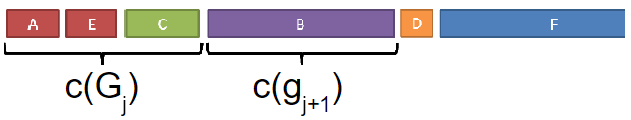
\includegraphics[width=0.8\textwidth]{\GOMPDIR/img/all-budget-good.png}
  \label{fig:all-budget-good}
}

\subfloat[Illustration of Doubling Algorithm Cost Constraint]{
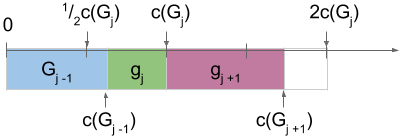
\includegraphics[width=0.8\textwidth]{\GOMPDIR/img/doubling-algo.png}
  \label{fig:doubling-algo}
}

\caption{Doubling Algorithm (b) has better anytime behaviors 
than greedy algorithm with no cost constraints (a).}
\label{fig:doubling}
\end{figure}


\begin{algorithm}[tb]
\caption{Forward Regression with Doubling Modification}
 \label{alg:greedy.doubling}
\begin{algorithmic}[1]
	\STATE {\bfseries Input:} Objective function $F$, elements $X$, minimum cost $c_{\textrm{min}}$.
	\STATE {\bfseries Output:} A sequence $G = g_1, g_2, ..., g_{J}$ of elements.
   For each $j \leq J$, a parameter  $w(G_j)$ for the elements $G_j =g_1,..., g_j$ for maximizing $F$. 
    \STATE Set $g_1 = \underset{x \in X,\ c(x) \le c_{\textrm{min}}}{\argmax} \frac{F(\{x\})}{c(x)}$.
    \STATE Set $G_1 = [g_1]$ as a one-element sequence.
    \STATE Set $w(G_1)$ be the parameter associated with $g_1$ to optimize $F$.
 \FOR {$j = 2,...,J$}
    \FOR {$g \notin G_{j-1}$, $c(g) \le c(G_{j-1})$}
        \STATE Compute $F(G_{j-1} \oplus g)$ and the associated parameter $w(G_{j-1} \oplus g)$.  
    \ENDFOR
    \STATE $g_{j} = \argmax \limits_{g = \mathcal{G}_1, ... , \mathcal{G}_J, g\notin G_{j-1}, c(g) \le c(G_{j-1})} 
	\frac{F(G_{j-1} \oplus g) - F(G_{j-1})}{c(g)}$.
   \STATE Append $g_j$ to the sequence: $G_{j} = G_{j-1} \oplus g_{j}$.
   \STATE Record $w(G_j) = w(G_{j-1} \oplus g)$.
 \ENDFOR
\end{algorithmic}
\end{algorithm}

 
\begin{definition} 
\label{def:greedy.doubling-capable}
Let $G = (g_1, \ldots)$ be the sequence selected by the doubling
algorithm.  The set $X$ and function $F$ are \textit{doubling capable}
if, at every iteration $j$, the following set is non-empty:
$
\{x \mid x \in X \setminus G_{j-1},\ c(x) \le c(G_{j-1})\}
$
\end{definition}

\begin{theorem}
\label{thm:greedy.doubling-greedy-bound-approx}
Let $G = (g_1, \ldots)$ be the sequence selected by the doubling
algorithm (Algorithm~\ref{alg:greedy.doubling}).  Fix some $B >
c_{\textrm{min}}$.  Let $F$ be $\gamma$-approximately
submodular as in Definition~\ref{def:greedy.approx-submodularity}.
For any sequence $S$,
\[
F(G_{\at{B}}) > \left(1 - e^{-\frac{\gamma^2}{1+\gamma}} \right) F(S_{\at{\frac{B}{4}}}).
\]
\end{theorem}
\begin{proof}
Doubling capable easily leads to the observation that for all budgets $B$, there exists an index $j$ such that
$\frac{B}{2} \leq c(G_j) < B$.
Choose $K$ and $k$ to be  the largest integers such that
$\frac{B}{2} \leq c(G_K) < B$ and 
$\frac{B}{8} \leq c(G_k) < \frac{B}{4}$. Since at each step we at most double the 
total cost and $4c(G_k) < B$, we observe $K \geq k+2$. 
%Let $\Delta C$ denote the cost difference $c(G_K) - c(G_k)$.
For each $j$, define $s_j = \frac{F(G_{j+1}) - F(G_{j})}{c(g_{j+1})}$ as the best 
rate of improvement among the items Doubling Algorithm is allowed to consider
after choosing $G_j$. 
Consider the item $x$ in sequence $S_{\at{\frac{B}{4}}}$ of the maximum cost. 

(Case 1) If $c(x) \leq c(G_k)$, then
every item in $S_{\at{\frac{B}{4}}}$ was a candidate for $g_{j}$ for all $j=k+1,..., K$. 
So by approximate submodularity from Equation~\ref{def:greedy.approx-submodularity}, we have 
\begin{align}
\label{eq:sub-additive}
F(S_{\at{\frac{B}{4}}}) \leq F(S_{\at{\frac{B}{4}}} \cup G_{j}) \leq F(G_j) + \frac{B s_j}{4 \gamma}.
\end{align}
Then using the standard submodular maximization proof technique, we define
\mbox{$\Delta _j = F(S_{\at{\frac{B}{4}}}) - F(G_j)$}. Applying $s_j = \frac{\Delta _{j} - \Delta_{j+1}}{c(g_{j+1})}$ in the above inequality, 
we have
\mbox{$\Delta _{k+j} \leq \Delta_k \prod _{j=k+1}^{k+j} ( 1 - \gamma \frac{ 4 c(g_{j})}{B})$}. Maximizing the 
inequality by setting $c(g_{j}) = \frac{B}{K-k} \leq \frac{c(G_K) - c(G_k)}{4 (K-k)}$, 
and using $(1- z/l)^l < e^{-z}$, we have 
\mbox{$F(G_K) > (1 - e^{-\gamma}) F(S_{\at{\frac{B}{4}}}).
$}

From now on, we assume that $c(x) > c(G_k)$ and consider 
two cases by comparing $c(g_{k+2})$ and $c(G_{k})$. 

(Case 2.1) If $c(g_{k+2}) \geq c(G_{k})$, then 
$c(G_K) - c(G_{k+1}) \geq c(g_{k+2}) \geq c(G_k)$. 
Since $c(G_{k+1}) \leq 2 c(G_k)$ and $c(x) > c(G_k)$, 
we have $c(G_K) - c(G_{k+1}) \geq \frac{B}{2} - 2c(G_k)$.
So \mbox{$c(G_K) - c(G_{k+1}) \geq \max ( c(G_k), \frac{B}{2} - 2c(G_k) ) \geq \frac{B}{6}$}. 
Thus, using the same proof techniques as in case 1, we can analyze the ratio between $\Delta_{k+1}$ and $\Delta_K$, and have:
\mbox{$
F(G_K) > (1 - e^{-\frac{2}{3} \gamma}) F(S_{\at{\frac{B}{4}}}).
$}

(Case 2.2) 
Finally, if \mbox{$c(g_{k+2}) < c(G_k) < c(x) < c(G_{k+1})$},
$g_{k+2}$ was a candidate for $g_{k+1}$, and $x$ was a candidate for 
$g_{k+2}$. 
For an item $y$, let 
\mbox{$r(y^j)= \frac{F(G_{j} \cup \{ y \}) - F(G_j)}{c(y)}$} 
be the improvement rate of item $y$ at $G_j$. 
Then we have \mbox{$r(g_{k+1}^k) > r(g_{k+2}^k)$} and \mbox{$r(g_{k+2}^{k+1}) > r(x^{k+1})$}. 
Since the objective function is increasing, we have 
\mbox{$r(x^k) c(x) \leq r(x^{k+1})c(x) + r(g_{k+1}^k)c(g_{k+1})$},
so that 
\mbox{$r(x^k) \leq r(x^{k+1}) + r(g_{k+1}^k) \frac{c(g_{k+1})}{c(x)}$}.
Then by the definition of $\gamma$ in Equation~\ref{def:greedy.approx-submodularity}, we have 
$ \gamma r(g^{k+1}_{k+2}) \leq r(g_{k+2}^k)$. Hence we have 
$ \gamma r(x^{k+1}) \leq  r(g_{k+1}^k)$, which leads to 
\mbox{$r (x^k) \leq r(g_{k+1}^k) (\frac{1}{\gamma} + \frac{c(g_{k+1})}{c(x)} ) \leq r(g_{k+1}^k) (1 + \frac{1}{\gamma})$}. Then
inequality~(\ref{eq:sub-additive}) holds with a coefficient adjustment and becomes
$
F(S_{\at{\frac{B}{4}}}) \leq F(G_k) + \frac{B s_k (1+\gamma)}{4 \gamma^2}.
$
Noting that the above inequality holds for all $j=k+1, ..., K$, we can replace the constant $\gamma$ in the 
proof of case $1$ with $\frac{\gamma^2}{1+\gamma}$ and have the following bound:\mbox{
$
F(G_K) > (1 - e^{-\frac{\gamma^2}{1+\gamma} }) F(S_{\at{\frac{B}{4}}}).
$}

\end{proof}


% terms, assumption, lemma
% Proof of the main lemma;

\section{EXPERIMENTS}
\label{sec:experiment}

\begin{table*}
\caption{Test time 0.97-Timeliness measurement of different methods on \Grain. We break
 the methods into OMP, FR and Oracle family: e.g., ``Single" in the G-CS-OMP family means G-CS-OMP-Single, and ``FR" in the Oracle family means the oracle curve derived from G-FR. }
\label{tab:grain_auc} 
\begin{center}
\resizebox{\textwidth}{!}{
\begin{tabular}{cccc|c|cc|c}
\multicolumn{4}{c|}{CS-G-OMP-Variants} &
\multicolumn{1}{c|}{CS-G-FR} &
\multicolumn{2}{c|}{Oracles} &
\multicolumn{1}{c}{Sparse} \\
	CS-G-OMP & 
	Single & 
	No-Whiten & 
	G-OMP & 
	\; & 
	FR Oracle &
	OMP Oracle &
  \; \\
  \hline
	\textbf{0.4406} & %G-OMP & 
	0.4086 &%G-OMP-Single & 
	0.4340 &%G-OMP-No-Whiten & 
	0.4073 &%G-OMP-Ignore-Cost & 
	\textbf{0.4525} &%G-FR 		& 
	\textbf{0.4551} & %FR Oracle \\
	0.4508 & % OMP oracle
  0.3997 \\
\end{tabular}
}
\end{center}
\end{table*}

\begin{table*}
\caption{Test time 0.99-Timeliness measurement of different methods on \YahooLTR.}
\label{tab:yahoo_auc} 
\begin{center}
\resizebox{\textwidth}{!}{
\begin{tabular}{c|cccc|c|cc|c}
Group &
\multicolumn{4}{c|}{CS-G-OMP-Variants} &
\multicolumn{1}{c|}{CS-G-FR} &
\multicolumn{2}{c|}{Oracles} &
\multicolumn{1}{c}{Sparse} \\
	Size &
	CS-G-OMP & 
	Single & 
	No-Whiten & 
	G-OMP & 
	\; & 
	FR &
	OMP &
  \; \\
\hline
	5      & %Group Size
	\textbf{0.3188} & %G-OMP & 
	0.3039 &%G-OMP-Single & 
	0.3111 &%G-OMP-No-Whiten & 
	0.2985 &%G-OMP-Ignore-Cost & 
	\textbf{0.3222} &%G-FR 		& 
	\textbf{0.3225} & % FR oracle
	0.3211 & %Oracle \\  
  0.2934 \\

	10      & %Group Size
	\textbf{0.3142} & %G-OMP & 
	0.3117 &%G-OMP-Single & 
	0.3079 &%G-OMP-No-Whiten & 
	0.2909 &%G-OMP-Ignore-Cost & 
	\textbf{0.3205} &%G-FR 		& 
	\textbf{0.3207} & % FR oracle
	0.3164 & %Oracle \\  
  0.2858 \\

	15      & %Group Size
	\textbf{0.3165} & %G-OMP & 
	0.3159 &%G-OMP-Single & 
	0.3116 &%G-OMP-No-Whiten & 
	0.2892 &%G-OMP-Ignore-Cost & 
	\textbf{0.3213} &%G-FR 		& 
	\textbf{0.3213} & % FR oracle
	0.3177 & %Oracle \\  
  0.2952 \\

	20     & %Group Size
	\textbf{0.3161} & %G-OMP & 
	0.3124 &%G-OMP-Single & 
	0.3065 &%G-OMP-No-Whiten & 
	0.2875 &%G-OMP-Ignore-Cost & 
	\textbf{0.3180} &%G-FR 		& 
	\textbf{0.3180} & % FR oracle
	0.3163 & %Oracle \\ 
  0.2895 \\

\end{tabular}
}
\end{center}
\end{table*}


\begin{figure}[ht!]
\centering
\subfloat[Training Time OMP vs. FR (\Grain)]{
  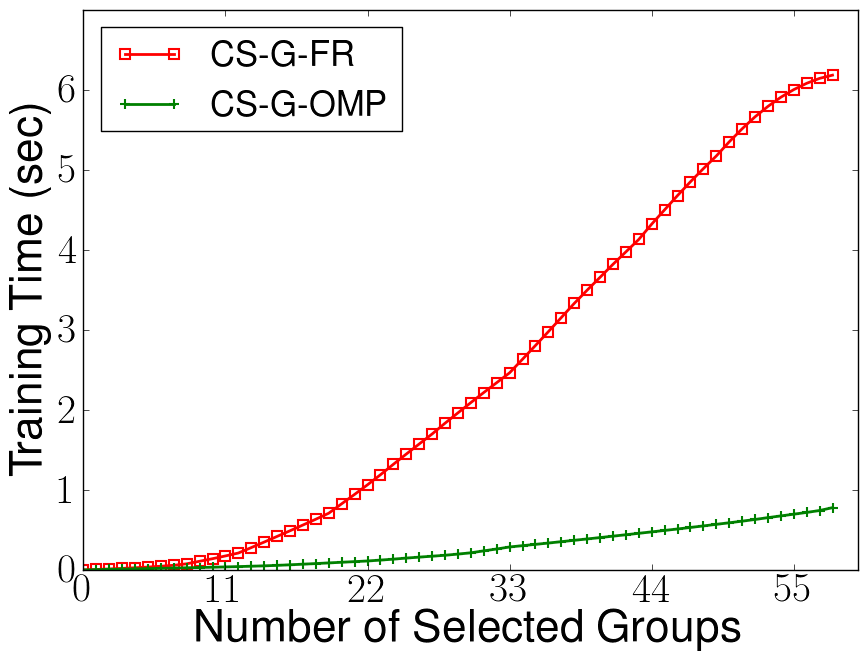
\includegraphics[width=0.44\textwidth,keepaspectratio]{\GOMPDIR/img/set1_exp4.png}
}
~
\subfloat[Training Time OMP vs. FR (\YahooLTR)]{
  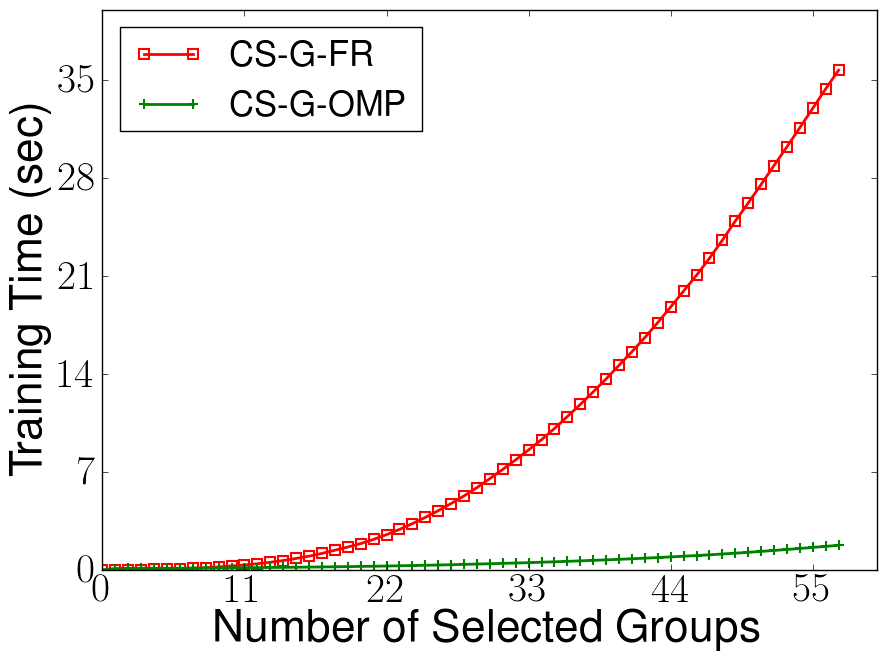
\includegraphics[width=0.44\textwidth,keepaspectratio]{\GOMPDIR/img/set1_size10_exp4.png}
}
\caption{The training time vs. the number of feature groups selected with two algorithms: CS-G-FR and 
CS-G-OMP. CS-G-OMP achieves a 8x and 20x overall training time speed-up 
on \Grain\, and \YahooLTR.} 
\label{fig:run_time}
\end{figure}

\subsection{DATA-SETS AND SET-UP}
We experiment our methods for anytime linear prediction on two real-world data-sets,
each of which has a significant number of feature groups with associated costs. 

\begin{itemize}[leftmargin=*]
\item \textbf{Yahoo! Learning to Rank Challenge} \citep{yahoo_ltr}
contains 883k web documents, each of which has a relevance score in $\{0, 1, 2, 3, 4\}$. Each of the 501 document features has an associated computational cost in 
$\{ 1, 5, 20, 50, 100, 150, 200\}$; the total feature cost is around 17K. The original data-set has no feature group structures, so we generated random group structures by grouping features of the same cost into groups of a given size $s$.\footnote{We experiment on group sizes $s \in \{ 5, 10, 15, 20 \}$. We choose regularizer 
$\lambda = 10^{-5}$ based on validation. We use 
$s=10$ for qualitative results such as plots and illustrations, but we report quantitative results for all group size $s$. For our quantitative results, we report the average test performance. The initial risk is $R(\emptyset)=0.85$.}

\item \textbf{Agriculture} is a proprietary data-set that contains 510k data samples, 328 features, and 57 feature groups. Each sample has a binary label in $\{1, 2\}$. Each feature group has an associated cost measured in its 
average computation time.\footnote{
There are 6 groups of size 32; the other groups have sizes between 1 and 6. 
The cost of each group is its expected computation time in seconds, ranging between 0.0005 and 0.0088; the total feature cost is 0.111. 
We choose regularizer $\lambda = 10^{-7}$. The data-set is 
split into five 100k sets, and the remaining 10k are used for validation. We report the cross validation results on the five 100K sets as the test results. The initial risk is $R(\emptyset) = 0.091$.}
\end{itemize}

\subsection{EVALUATION METRIC, BASELINE AND ORACLE}
\label{sec:timeliness}
\begin{figure}[ht!]
\centering
\subfloat[Plateau Effect and $\alpha$-Stopping Costs]{
 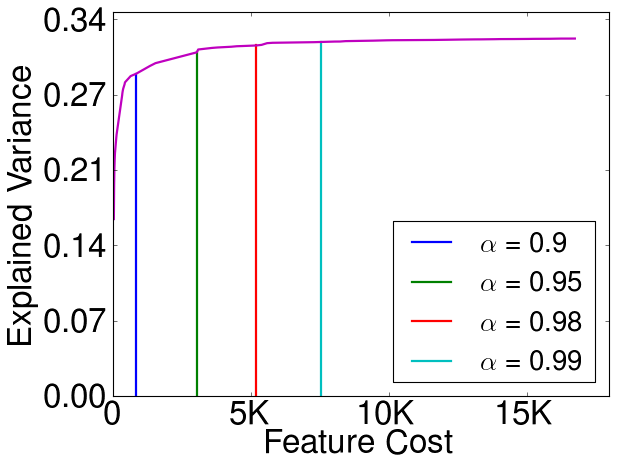
\includegraphics[width=0.44\textwidth,keepaspectratio]{\GOMPDIR/img/timeliness.png}
 \label{fig:timeliness_a}
}
~
\subfloat[Importance of Costs (CS-G-OMP vs. G-OMP)]{
 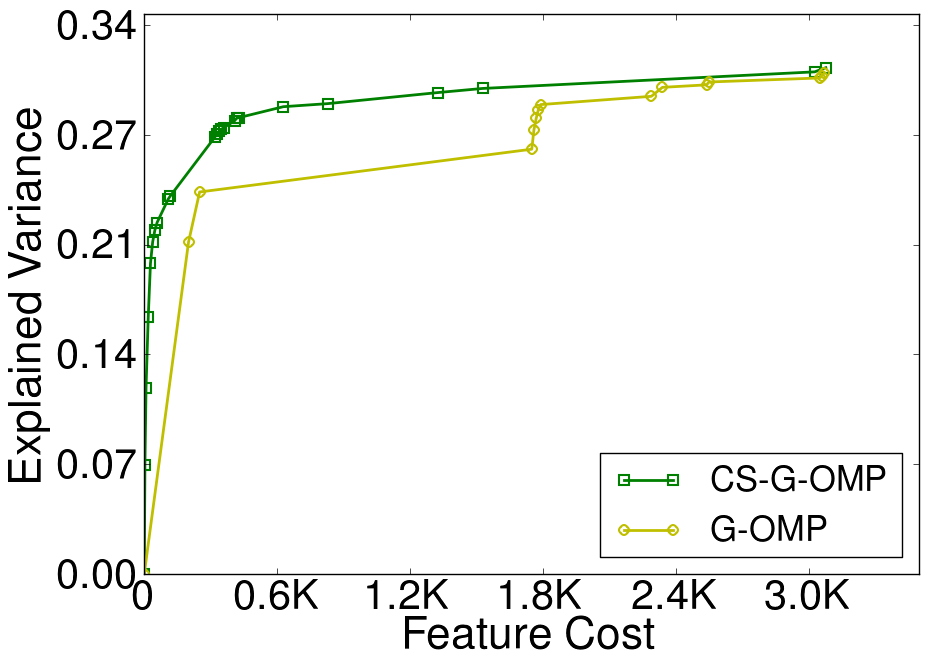
\includegraphics[width=0.44\textwidth,keepaspectratio]{\GOMPDIR/img/set1_size10_exp2.png}
 \label{fig:cost_vs_no_cost}
}
\label{fig:timeliness}
\caption{(a) Explained Variance vs. Cost curve of CS-G-OMP in
\YahooLTR. Vertical lines mark different $\alpha$-stopping costs.  (b) Explained Variance vs. Cost curve of CS-G-OMP and G-OMP on \YahooLTR\, set 1 with individual group size $s=10$, stopped at 0.97-stop cost.}
\end{figure}

Following the practice of \cite{timeliness}, we use the area under the 
maximization objective $F$ (explained variance) vs. cost curve normalized by the total area as the 
\textit{timeliness} measurement of the anytime performance of an algorithm\footnotetext{\cite{timeliness} define \textit{timeliness} as the area under the average precision vs. time curve}. In our data-sets, the performance of linear predictors plateaus much before
all features are used, e.g., Figure~\ref{fig:timeliness_a} demonstrates this effect in \YahooLTR, where the last one percent of total improvement is bought by half of the total feature cost. Hence the majority of the timeliness measurement is from the plateau performance of linear predictors. The difference between timeliness of different anytime algorithms diminishes due to the plateau effect. Furthermore, the difference vanishes as we include additional redundant high cost features. To account for this effect, we 
stop the curve when it reaches the plateau.
We define an \textit{$\alpha$-stopping cost} for parameter $\alpha$ in $[0,1]$ as the cost at which our CS-G-OMP achieves $\alpha$ of the final objective value in training and ignore the objective vs. cost curve after
the $\alpha$-stopping cost. We call the timeliness measure on the shortened curve 
as \textit{$\alpha$-timeliness}; 1-timeliness equals the normalized area under the full curve and 0-timeliness is zero. If a curve does not pick a group at $\alpha$-stopping cost, we linearly interpolate the objective value at the stopping cost to 
computr timeliness. 
We say an objective vs. cost curve has reached its final plateau if at least 95\% of the total 
objective has been achieved and the next 1\% requires more than 20\%
feature costs. (If the plateau does not exist, we use $\alpha = 1$.) Following this rule, we choose $\alpha = 0.97$ for \Grain\ and $\alpha = 0.99$ for \YahooLTR.

Since an exhaustive search for the best feature sequencing is intractable, 
we approximate with the \textbf{Oracle} anytime performance following the approach of \cite{timeliness}. Given an objective vs. cost curve of a sequencing, we reorder the feature groups in descending order of their marginal benefit per unit cost, assuming that the marginal benefits stay the same after reordering. We specify which sequencing is used for creating \textbf{Oracle} in Section~\ref{sec:selection_methods}. 
For baseline performance, we use cost-weighted Group Lasso \citep{group_lasso}, which
scales the regularization constant of each group with the cost of the group. We note that the cascade design by 
\cite{chen:12} can be reduced to this baseline if we enforce
linear prediction. 
More specifically, the baseline solves the following minimization problem:
\mbox{$
  \min _{w \in \mathbb{R}^{D}} \Vert Y -
    Xw \Vert^2_2 + \lambda
    \sum _{j=1}^J c(\mathcal{G}_j) \Vert w _{\mathcal{G}_j} \Vert _2,
$}
and we vary value of regularization constant
$\lambda$ to obtain lasso paths. We call this baseline algorithm \textbf{Sparse}\footnote{We use an off-the-shelf software, 
SPAMS (SPArse Modeling Software \citep{spams}), to solve the optimization.}.


\subsection{FEATURE COST}
Our proposed CS-G-OMP differs from Group Orthogonal Matching Pursuit (G-OMP) \citep{gomp} in that G-OMP does not consider feature costs when evaluating features. We show that this difference is crucial for anytime linear prediction. In Figure~\ref{fig:cost_vs_no_cost}, we compare the objective vs. costs curves of CS-G-OMP and G-OMP that are stopped at 0.97-stopping cost on \YahooLTR. As expected, CS-G-OMP achieves a
better overall prediction at every budget, qualitatively demonstrating the importance of incorporating feature costs. Table~\ref{tab:grain_auc} and Table~\ref{tab:yahoo_auc} 
quantify this effect, showing that CS-G-OMP 
achieves a better timeliness
measure than regular G-OMP. 

\subsection{GROUP WHITENING}
%Compare different normalization methods: whiten the whole data, 
%zero mean normalize, whiten each group. \and 
We provide experimental evidence that  
Group whitening, i.e., $X_g^TX_g = I_{D_g}$ for each group $g$, is a key assumption of both this work and previous feature group selection literature  by \cite{gomp, log_gomp}.
In Figure~\ref{fig:whiten_vs_no_whiten}, we compare 
anytime prediction performances using group whitened data 
against those using the common  
normalization scheme where each feature dimension
is individually normalized to have zero mean and unit variance. 
The objective vs. cost curve qualitatively shows that group whitening consistently results in the better predictions.
This behavior is expected from data-sets whose feature groups contain correlated features, e.g., group whitening effectively prevents selection step $(*)$ from overestimating the predictive power of feature groups of repeated good features. Table~\ref{tab:grain_auc} and Table~\ref{tab:yahoo_auc} demonstrate quantitatively the consistent better timeliness performance of CS-G-OMP over that of CS-G-OMP-no-whiten. 


\begin{figure}[ht!]
\centering
\subfloat[Group Whiten vs. No-Whiten (\Grain)]{
  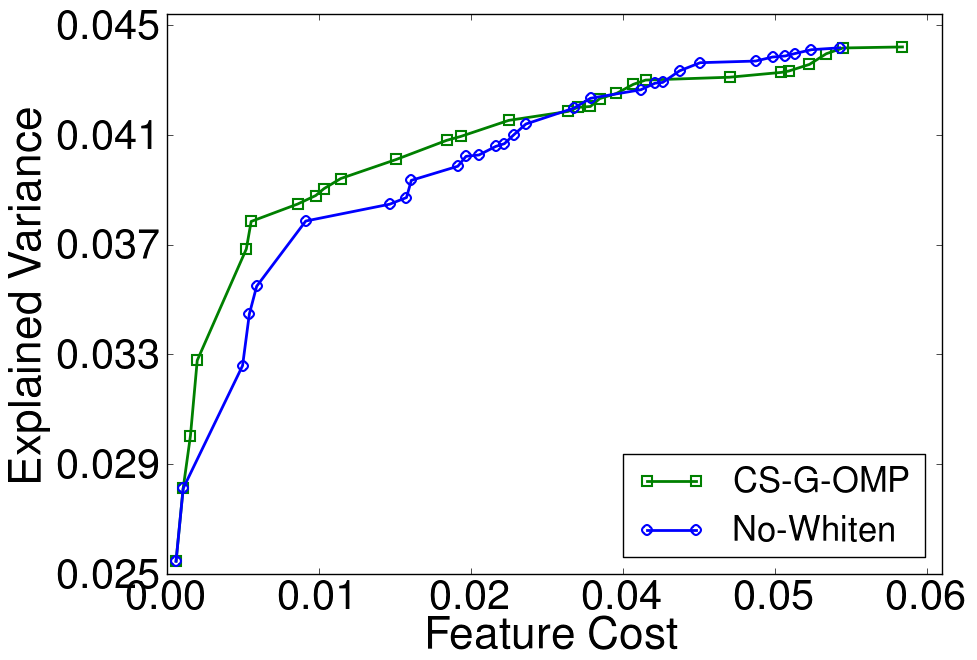
\includegraphics[width=0.44\textwidth,keepaspectratio]{\GOMPDIR/img/set1_exp1.png}
}
~
\subfloat[Group Whiten vs. No-Whiten (\YahooLTR)]{
  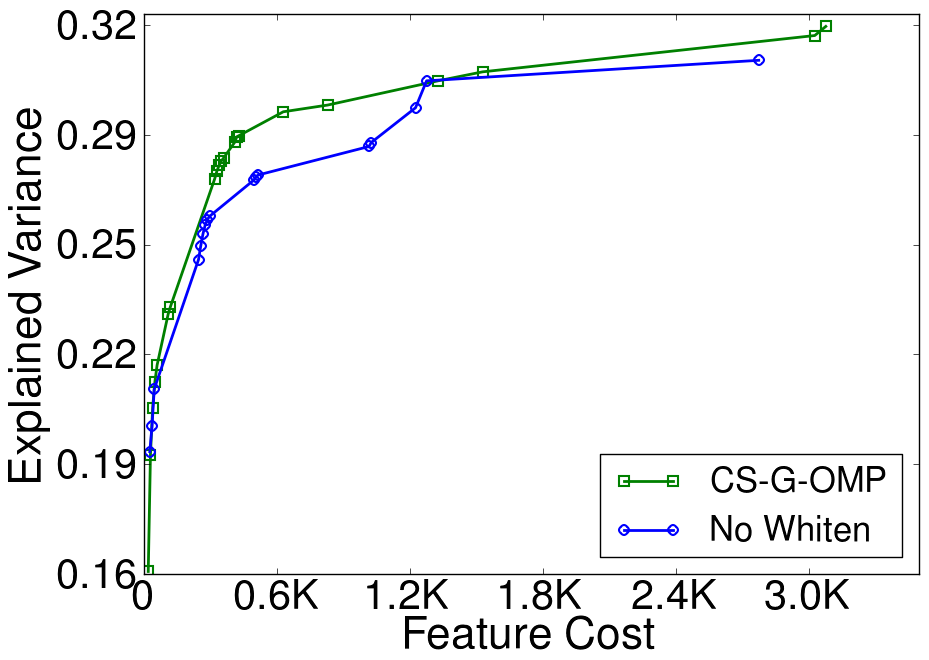
\includegraphics[width=0.44\textwidth,keepaspectratio]{\GOMPDIR/img/set1_size10_exp1.png}
}
\caption{Explained Variance vs. Feature Cost curves on \Grain\, (a) and \YahooLTR\, (b)  comparing group whitening with no group whitening. The curves stop at 0.97-stopping cost.}
\label{fig:whiten_vs_no_whiten}
\end{figure}


\subsection{SELECTION CRITERION VARIANTS}
\label{sec:selection_methods}
%FR vs OMP; group vs single

This section compares CS-G-OMP and CS-G-FR, along with 
variants of these two methods and the baseline, Sparse. 
We formulated the variant of CS-G-OMP, \textit{single}, in Section~\ref{sec:gomp_method} and it intuitively chooses feature groups of the best single feature dimension per group cost. Our experiments show that this modification degrades prediction performance of CS-G-OMP. 
%If we enforce linear prediction, cascade design by \cite{cai:15} can be reduced to a greedy method whose criteria is the G-OMP criteria subtracted by a function of the feature cost. However, this method requires careful tuning of the 
Since FR directly optimizes the objective at each step, we expect CS-G-FR to perform the best and use its curve to compute the \textbf{Oracle} curve as an approximate to the best achievable performance.

In Figure~\ref{fig:selection_methods}, we evaluate CS-G-FR, CS-G-OMP and CS-G-OMP-single based on the objective in Theorem~\ref{thm:main}, i.e., explained variance vs. feature cost curves. 
CS-G-FR, as expected, outperforms all other methods. CS-G-OMP outperforms the baseline method, Sparse, and the CS-G-OMP-Single variant. 
The performance advantage of CS-G-OMP over CS-G-OMP-Single is much clearer in the \Grain\ data-set than in the \YahooLTR\ data-set. \Grain\ has a natural group structure which may contain correlated features in each group. \YahooLTR\ has a randomly generated group structure whose features were filtered by feature selection before the data-set was published \citep{yahoo_ltr}. CS-G-FR and CS-G-OMP outperform the baseline algorithm, Sparse. We speculate that linearly scaling group regularization constants by group costs did not enforce Group-Lasso to choose the most cost-efficient features early. 
The test-time timeliness measures of each of the methods are recorded in Table~\ref{tab:grain_auc} and Table~\ref{tab:yahoo_auc},
and quantitatively confirm the analysis above. Since \Grain\, and \YahooLTR\, are originally a classification and a ranking data-set, respectively, we also report in Figure~\ref{fig:selection_methods} the performance using classification accuracy and NDCG@5. This demonstrates the same qualitatively results as using explained variants. 

%We note that on the two real-world data-sets, Doubling Algorithm acts identically to CS-G-FR after few initial selections, an expected result because real-world feature effectiveness does not grow exponentially in cost, so that the most cost-efficient features become available to Doubling after few steps. 


\begin{figure}[ht!]
\centering
\subfloat[FR vs. OMP vs. Sparse (\Grain)]{
  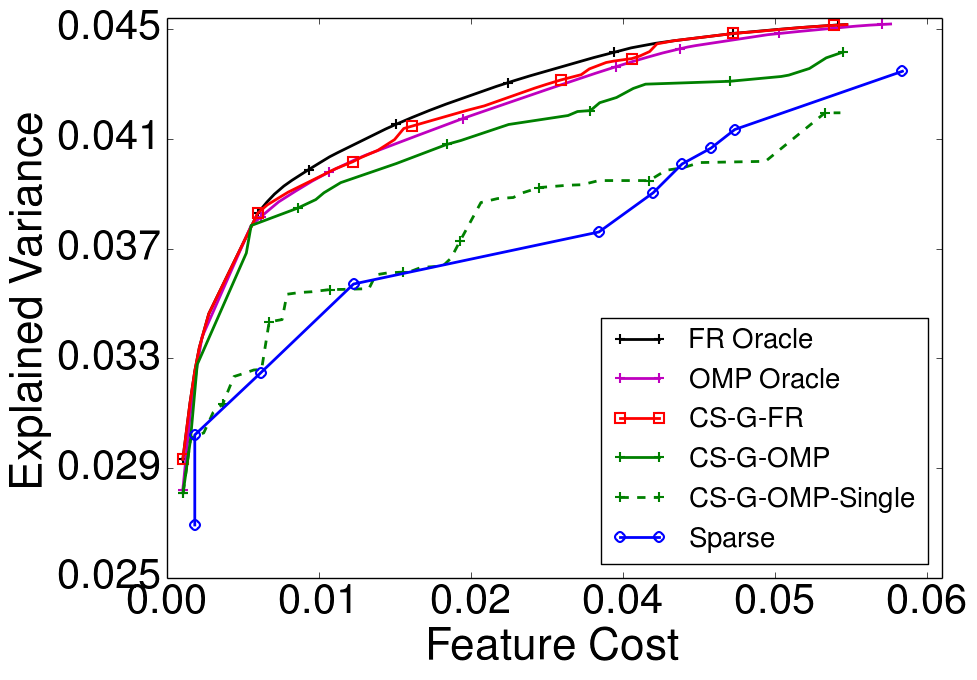
\includegraphics[width=0.44\textwidth,keepaspectratio]{\GOMPDIR/img/set1_exp3.png}
}
~
\subfloat[FR vs. OMP vs. Sparse (\YahooLTR)]{
  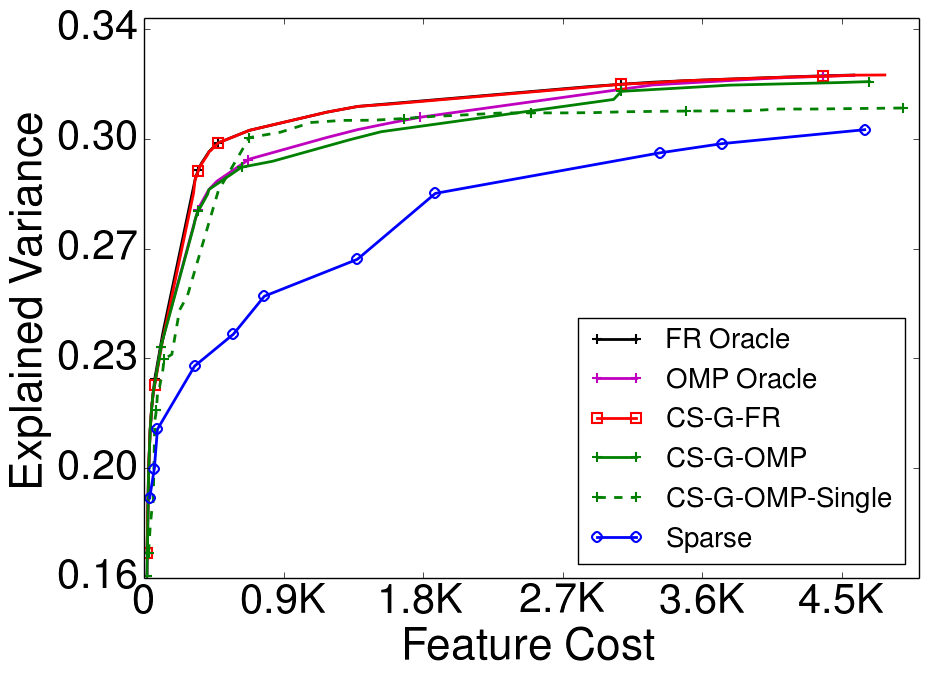
\includegraphics[width=0.44\textwidth,keepaspectratio]{\GOMPDIR/img/set1_size10_exp3.png}
}

\subfloat[FR vs. OMP vs. Sparse (\Grain)]{
  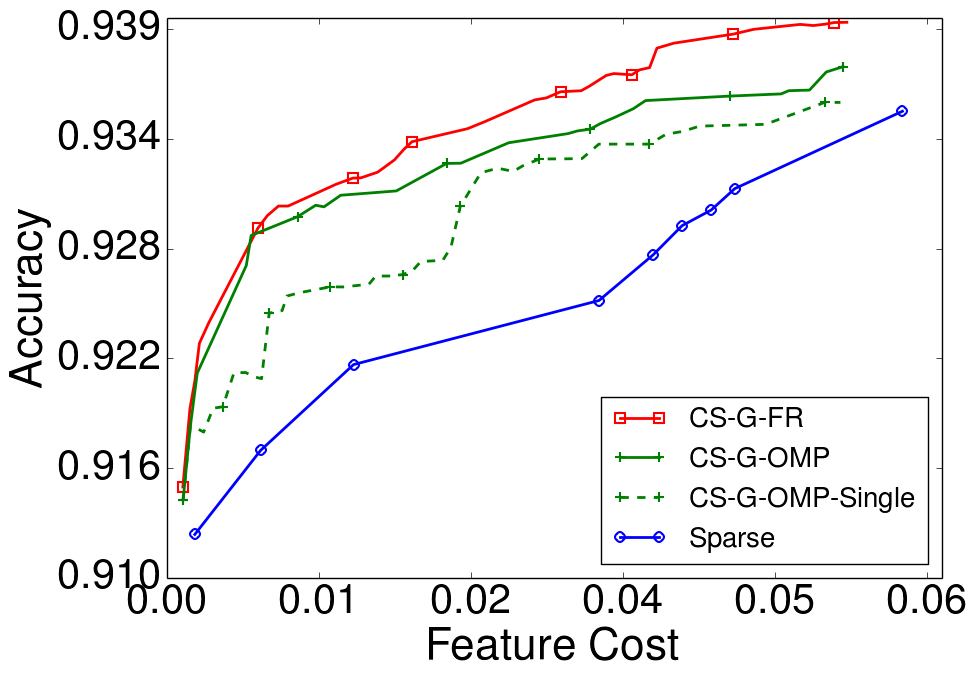
\includegraphics[width=0.44\textwidth,keepaspectratio]{\GOMPDIR/img/set1_exp5.png}
}
~
\subfloat[FR vs. OMP vs. Sparse (\YahooLTR)]{
  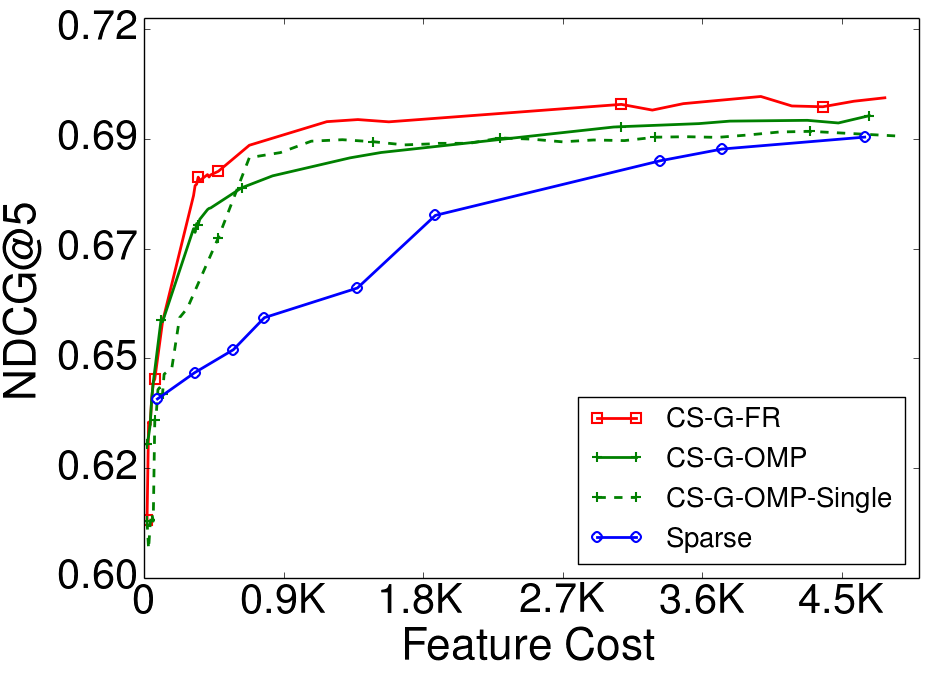
\includegraphics[width=0.44\textwidth,keepaspectratio]{\GOMPDIR/img/set1_size10_exp5.png}
}

\caption{(a),(b): Explained Variance vs. Feature Cost curves on 
\Grain\, and \YahooLTR (group-size=10), 
using CS-G-OMP, CS-G-FR and their Single variants. Curves stop at 0.97 and 0.98 stopping costs. (c),(d): Same curve with the natural objectives of the data-sets: accuracy and NDCG@5.} 
\label{fig:selection_methods}
\end{figure}

As expected, when compared against CS-G-OMP, CS-G-FR consistently chooses more cost-efficient features at the cost of a longer training time.
In the context of linear regression, let us assume that the group sizes are 
bounded by a constant when we are to select the number 
$K$ feature group. We can then compute a new model of $K$  groups in $O(K^2N)$ using
Woodbury's matrix inversion lemma, evaluate it in $O(KN)$, and compute the gradients with respect to the weights of unselected groups in $O(N(J-K))$. Thus, CS-G-OMP requires $O(K^2N + JN)$ at step $K=1,2,3,..., J$ and CS-G-FR requires $O((J-K)K^2N)$, so the total training  complexities for CS-G-OMP and CS-G-FR are $O(J^3N)$ and $O(J^4N)$, using $\sum_{K=1}^J K^2 = \frac{1}{6}J(J+1)(2J+1)$ and $\sum _{K=1}^J K^3 = \frac{1}{4}J^2(J+1)^2$. 
We also show this training complexity gap empirically in Figure~\ref{fig:run_time}, which plots the curves of training time vs. number of feature groups selected. When all feature groups are selected, CS-G-OMP achieves a 8x speed-up in \Grain\ over CS-G-FR. In \YahooLTR, CS-G-OMP achieves a speed-up factor between 10 and 20; the smaller the sizes of the groups, the larger speed-up due to the increase in the number of groups. Both greedy methods are much faster than the Lasso path computation using SPAMS, however. 






\section{Additional Proof Details}
\label{sec:gomp_proof_II}
This section describes a functional boosting view of selecting features for generalized linear models of one-dimensional response. We then prove Lemma~\ref{lemma:smoothness} and Lemma~\ref{lemma:convexity} for this more general setting. These more general
results in turn extend Theorem~\ref{thm:main} to generalized 
linear models.

\subsection{Functional Boosting View of Feature Selection}
\label{sec:functional}

We view each feature $f$ as a function 
$h_f$ that maps sample $x$ to $x_f$. We define $f_S: \R^{D} \rightarrow \R$ 
to be the best linear predictor using features in $S$, i.e., $f_S(x) \triangleq w(S)^Tx_S$. For each feature dimension $d \in D$, the coefficient of 
$d$ is in $w(S)$ is $w(S)_d = f_S(e_d)$, where $e_d$ is the $d^{th}$ dimensional unit vector. So $\Vert w(S) \Vert_2^2 = \sum _{d = 1}^D \Vert f_S(e_d) \Vert _2^2$. 
Given a generalized linear model with link function $\nabla \Phi$, 
the predictor is $E[ y | x ] = \nabla \Phi(w^Tx)$ for some $w$ and the calibrated loss is $r(w) = \sum _{i=1}^n (\Phi(w^Tx_i) - y_iw^Tx_i)$. 
Replacing $f_S(x_i) = w(S)^Tx_i$, we have 
\begin{align}
	r(w(S)) = \sum _{i=1}^n (\Phi(f_S(x_i)) - y_if_S(x_i)).
	\label{eq:glm_loss_general}
\end{align}
Note that the risk function in Equation~\ref{eq:risk} can be rewritten as 
the following to resemble Equation~\ref{eq:glm_loss_general}:
\begin{align}
 R(S) = 
 	\mathcal{R}[f_S] =& \frac{1}{n} \sum _{i=1}^n (\Phi(f_S(x_i)) - y_i^Tf_S(x_i)) \notag \\
    &{} + \frac{\lambda}{2} \sum _{d = 1}^D \Vert f_S(e_d) \Vert _2^2 + A,
  \label{eq:min_func}
\end{align}
where $\phi(x) = \frac{1}{2}x^2$ for linear predictions and constant 
$A = \frac{1}{2n} \sum _{i=1}^n y_i^2$. 
Next we define the inner product between two functions $f, h : \R^D \rightarrow \R$ 
over the training set to be:
\begin{align}
\angleb{f, h} \triangleq \frac{1}{n} 
  \sum _{i=1}^n f(x_i)h(x_i) + \frac{\lambda}{2} \sum _{d=1}^D f(e_d)h(e_d).
\end{align}
With this definition of inner product, we can compute the derivative of 
$\mathcal{R}$:
\begin{align}
  \nabla \mathcal{R}[f]  = \sum_{i=1}^n (\nabla\Phi(f(x_i)) 
  	- y_{i})\delta_{x_i} 
    + \sum _{d=1}^D f(e_d)\delta_{e_d},
\end{align}
where $\nabla \phi(x) = x$ for linear predictions, and 
$\delta_x$ is an indicator function for $x$. 
Then the gradient of objective $F(S)$ w.r.t coefficient $w_f$ of a feature dimension  $d$ can be written as:
\begin{align}
 b_{d}^S &= - \frac{1}{n}\sum_{i=1}^n (\nabla\Phi_p(w(S)^Tx^i) - y^{i})x^i_d - \lambda w(S)_d \\
    &= - \angleb{  \nabla \mathcal{R}[f_S], h_d }.
\end{align}
In addition, the regularized covariance matrix of features $C$ satisfies,
\begin{equation}
    C_{ij} = \frac{1}{n} X_i^TX_j + \lambda I(i=j) = \angleb{ h_i, h_j},
\end{equation}
for all $i, j = 1,2,..., D$.
So in this functional boosting view,  Algorithm~\ref{algo:gomp_lm} greedily chooses group $g$ that maximizes, with a slight abuse of notation of $\angleb{ \;, \; }$,
$\Vert \angleb{ h_g , \nabla \mathcal{R}[f_S] } \Vert _2^2 / c(g)$, i.e., 
the ratio between similarity of a feature group and the functional gradient, 
measured in sum of square of inner products, and the cost of the group


\subsection{Proof of Lemma~\ref{lemma:smoothness} and Lemma~\ref{lemma:convexity}}

The more general version of Lemma~\ref{lemma:smoothness} and Lemma~\ref{lemma:convexity} assumes that the objective functional $\mathcal{R}$ 
is $m$-strongly smooth and $M$-strongly convex using our proposed inner product rule.  
$M$-strong convexity is a reasonable assumption, 
because the regularization term $\Vert w \Vert _2^2 = \sum _{d = 1}^D \Vert f_S(e_d) \Vert _2^2$ ensures that all loss functional $\mathcal{R}$ with a convex $\Phi$ 
 strongly convex. 
In the linear prediction case, both $m$ and $M$ equals $1$. 

The following two lemmas are the more general versions of Lemma~\ref{lemma:smoothness} and Lemma~\ref{lemma:convexity}.
\begin{lemma}
  Let $\mathcal{R}$ be an m-strongly smooth functional with respect to our definition of inner products. Let $S$ and $G$ be some fixed sequences. Then
  \begin{align}
   F(S) - F(G) \notag \leq \frac{1}{2m} \angleb{b^G_{G \oplus S}, C_{G \oplus S}^{-1} b^G_{G\oplus S}}
  \end{align}
  \label{lemma:smoothness_glm}
\end{lemma}
\begin{proof}
First we optimize over the weights in $S$. 
  \begin{align*}
    &{} F(S) - F(G) \\
    &= \mathcal{R}[f_G] - \mathcal{R}[f_S] 
     = \mathcal{R}[f_G] - \mathcal{R}[\sum _{s \in S} \alpha_s^T h_s] \\
    &\leq \mathcal{R}[f_G] - \min _{w : w_i^T \in \R^{d_{s_i}}, s_i \in S} 
        \mathcal{R}[ \sum _{s_i \in S} w_{s_i}^T h_{s_i}] \\
\intertext{Adding dimensions in $G$ will not increase the risk, we have: }
    &\leq \mathcal{R}[f_G] - \min _{w : w_i \in \R^{d_{s_i}}, s_i \in G \oplus S}
        \mathcal{R}[ \sum _{s_i \in G \oplus S} w_{s_i} h_{s_i}] \\
\intertext{Since $f_G = \sum _{g_i \in G} \alpha_i h_{g_i}$, we have:}
    &\leq \mathcal{R}[f_G] - \min _{w} 
      \mathcal{R}[f_G + \sum _{s_i \in G \oplus S} w_i^T h_{s_i}] \\
\intertext{Expanding using strong smoothness around $f_G$, we have:}
    &\leq \mathcal{R}[f_G] - \min _{w} (
      \mathcal{R}[f_G] + \angleb{ \nabla \mathcal{R}[f_G], 
        \sum _{s_i \in G\oplus S} w_i^T h_{s_i} } \notag \\
    &\quad + \frac{m}{2} \Vert \sum _{s_i \in G \oplus S} w_i^T h_{s_i} \Vert _2^2) \\
    &= \max_{w} - 
      \angleb{ \nabla \mathcal{R}[f_G], 
      \sum _{s_i \in G\oplus S} w_i^T h_{s_i} } 
        - \frac{m}{2} \Vert \sum _{s_i \in G \oplus S} w_i^T h_{s_i} \Vert _2^2 \\
    &= \max_w \angleb{ b^{G}_{G\oplus S}, w} - \frac{m}{2} \angleb{w, C_{G\oplus S}w}
 \end{align*}
Solving $w$ directly we have:
\begin{align*}
  F(S) - F(G) \leq \frac{1}{2m} \angleb{ b^{G}_{G\oplus S} , C_{G\oplus S}^{-1} b^{G}_{G\oplus S}}
\end{align*}
\end{proof}


%%%%%%%%%%%%% 
%%%%%  Lemma Strong convexity
\begin{lemma}
  Let $\mathcal{R}$ be a M-strongly convex functional with respect to our definition of 
  inner products. Then
    \begin{align}
      F(G_j) - F(G_{j-1}) \geq \frac{1}{2M (1 + \lambda) } \angleb{{b^{G_{j-1}}_{g_j}}, b^{G_{j-1}}_{g_j} }
    \end{align}
  \label{lemma:convexity_glm}
\end{lemma}
\begin{proof}
After the greedy algorithm chooses some group $g_j$ at step $j$, 
  we form $f_{G_j} = \sum _{\alpha _i} \alpha_i^T h_{g_i}$, such that
   \[
    \mathcal{R}[f_G] = \min _{ \alpha _i \in \R^{d_{g_i}}} 
      \mathcal{R}[ \sum _{g_i \in G_j} \alpha_i^T h_{g_i}] \leq
      \min _{\beta \in \R^{d_{g_j}}} 
    \mathcal{R}[f_{G_{j-1}} + \beta h_{g_j}]
   \]
 Setting $\beta = \arg \min _{\beta \in \R^{d_{g_j}}} 
    \mathcal{R}[f_{G_{j-1}} + \beta h_{g_j}]$, using the strongly convex condition at
      $f_{G_{j-1}}$, we have:
 \begin{align*}
    &{} F(G_j) - F(G_{j-1}) \\
    &=  \mathcal{R}[f_{G_{j-1}}] - \mathcal{R}[f_{G_j}] 
    \geq \mathcal{R}[f_{G_{j-1}}] - \mathcal{R}[f_{G_{j-1}} + \beta h_{g_j}] \\ 
    &\geq  \mathcal{R}[f_{G_{j-1}}] - 
      (\mathcal{R}[f_{G_{j-1}}] + 
        \angleb{ \nabla \mathcal{R}[f_{G_{j-1}}] , 
        \beta h_{g_j} } \notag \\
    &\quad + \frac{M}{2} \Vert \beta h_{g_j} \Vert _2^2) \\
    &=  -  \angleb{ \nabla \mathcal{R}[f_{G_{j-1}}] , 
        \beta h_{g_j} }
       - \frac{M}{2} \Vert \beta h_{g_j} \Vert _2^2 \\
    &=  \angleb{{b^{{G_{j-1}}}_{g_j}},  \beta} - \frac{M}{2} \angleb{\beta, C_{g_j} \beta} \\
    &\geq  \frac{1}{2M} \angleb{ b^{{G_{j-1}}}_{g_j}, C_{g_j}^{-1} b^{{G_{j-1}}}_{g_j}} \\
    &=  \frac{1}{2M (1+\lambda)} \angleb{{b^{{G_{j-1}}}_{g_j}}, b^{{G_{j-1}}}_{g_j}}
 \end{align*}
 The last equality holds because each group is whitened, 
 so that $C_{g_j} = (1 + \lambda) I$.
\end{proof}
Note that the $(1+\lambda)$ constant is a result of group whitening, without which
the constant can be as large as $(D_{g_j} + \lambda)$ for  the worst case where
all the $D_{g_j}$ number of features are the same. \\

The proofs above for Lemma~\ref{lemma:smoothness_glm} and~\ref{lemma:convexity_glm} are 
for one-dimensional output responses. They can be easily generalized to multi-dimensional 
responses by replacing 2-norms with Frobenius norms and vector inner-products with ``Frobenius products", i.e., the sum of the products of all elements. \\

\subsection{Proof of Main Theorem}
\label{sec:app-main-proof}
Given Lemma~\ref{lemma:smoothness_glm} and Lemma~\ref{lemma:convexity_glm}, 
the proof of Lemma~\ref{lemma:main} holds with the same analysis with a more 
general constant $\gamma = \frac{m \lambda_{min}(C)}{M(1+\lambda)}$. The following prove our main theorem~\ref{thm:main}. 
 
\begin{proof} (of Theorem~\ref{thm:main}, given Lemma~\ref{lemma:main})
\label{proof:main}
  Define $\Delta _j = F(S_{\angleb{K}}) - F(G_{j-1})$. Then we have 
  $\Delta _j - \Delta_{j+1} = F(G_{j}) - F(G_{j-1})$. By Lemma ~\ref{lemma:main}, we have:
  \begin{align*}
    \Delta_j &= F(S_{\angleb{K}}) - F(G_{j-1})\\
    &\leq \frac{K}{\gamma}
      \lbrack \frac{F(G_{j}) - F(G_{j-1})}{c(g_{j})} \rbrack 
        = \frac{K}{\gamma} \lbrack \frac{\Delta_j - \Delta_{j+1}}{c(g_j)} \rbrack
  \end{align*}
  Rearranging we get 
    $\Delta_{j+1} \leq \Delta_j ( 1 - \frac{\gamma c(g_j)}{K} )$. Unroll we get:
  \begin{align*}
    \Delta _{L+1} 
    &\leq 
      \Delta _1 \prod _{j=1}^L (1 - \frac{\gamma c(g_j)}{K})
    \leq \Delta _1 ( \frac{1}{L} \sum _{j=1}^L (1- \frac{\gamma c(g_j)}{K})) ^L\\
    &= \Delta _1 (1 - \frac{B\gamma}{L K})^L < \Delta_1 e^{- \gamma \frac{B}{K}}
  \end{align*}
  By definition of $\Delta_1$ and $\Delta_{L+1}$, we have:
  \begin{align*}
    F(S_{\angleb{K}}) - F(G_{\angleb{B}}) < F(S_{\angleb{K}}) e^{- \gamma \frac{B}{K}}
  \end{align*}
  The theorem follows and linear prediction is the special case that $m = M$.
\end{proof}

%\section{Appendix B: Generalized Linear Model with Multi-Dimensional Response}
\section{Extension to Generalized Linear Model}
\label{sec:extension}
While we only formulated the feature group sequencing problem in linear prediction setting previously, we can extend our algorithm for generalized linear models\cite{glm} and multi-dimensional responses. In general, we assume that we have $P$ dimensional responses, and predictions are of the form $E[y | x ] = \nabla \phi( W x)$, for some known convex function $\phi : \mathbb{R}^P \rightarrow \mathbb{R}$, and an unknown coefficient $P\times D$ matrix, $W$. Thus, the generalized linear
prediction problem is to minimize over coefficient matrix $W: P\times D$:
\begin{align}
	\textbf{r}(W) = \frac{1}{n} \sum _{i=1}^n (\phi(Wx^i) - {y^i}^TWx^i) 
		+ \frac{\lambda}{2} \Vert W\Vert^2_F,
		\label{eq:glm_loss}
\end{align}
where $\lambda$ is the regularization constant for Frobenius norm of the coefficient 
matrix. In particular, we have $\phi(x) = \frac{1}{2}x^2$ for linear prediction. 
The risk of a collection of features, $S$, is then 
\mbox{$R(S) = \underset{W : \forall g \notin S  W_g = \textbf{0} }{\min} \textbf{r}(W)$}. 
To extend CS-G-OMP to feature sequencing in this general setting, we again, at each step,
take gradient of the objective $\textbf{r}$ w.r.t. $W$, and choose the feature group that has the largest ratio of group gradient Frobenius norm square to group cost. More specifically, after choosing groups in $G$, we have a best coefficient matrix restricted to G, $W(G)$. Then we compute the gradient w.r.t. $W$ at $W(G)$ (we keep the convention that unselected groups have zero coefficients) as:
\begin{align}
	\nabla \textbf{r}(W) = \frac{1}{n} \sum _{i=1}^n (\nabla \phi(Wx^i) - y^i){x^i}^T + \lambda W;
	\label{eq:glm_gradient}
\end{align}
we then evaluate $\Vert \textbf{r}(W)_g \Vert_F^2 / c(g)$ for each feature group $g$, and add the maximizer to the selected groups to create new models. 
Algorithm~\ref{algo:gomp_glm} demonstrates the procedure. 

Our theoretical result Theorem~\ref{thm:main} can also be proven in this general setting. 
Proofs of Lemma \ref{lemma:smoothness} and \ref{lemma:convexity}) in appendix are readily for generalized linear models\footnote{Inner products, $\angleb{\bullet, \bullet}$, in Lemma \ref{lemma:smoothness} and \ref{lemma:convexity} now represent Frobenius products, which are sums of element-wise products of matrices.}. Given these two lemmas, our proofs of Lemma~\ref{lemma:main}
and Theorem~\ref{thm:main} hold as they are. 


%%%%%%%%%%%%%%%%%%%%%%%%%
%% Algorithm statement %%
%%%%%%%%%%%%%%%%%%%%%%%%%
%\IncMargin{1em}
%\begin{algorithm}[h]
%  \SetKwInOut{Input}{input}\SetKwInOut{Output}{output}
%
%  \Input{The data matrix $\XX = [ \textbf{f}_1, ..., \textbf{f}_D ] \in \R^{n \times D}$,
%    with group structures, such that for each group $g$,
%    $\XX^T_{g}\XX_{g} = I _{D_g}$.     
%    The cost $c(g)$ of each group $g$. 
%    The response matrix $\YY \in \{0, 1\}^{n \times P}$.
%    The link function $\nabla \Phi$.
%    Regularization constant $\lambda$.
%  }
%  \Output{
%    A sequence $((G_j, W_j))_j$, where 
%      $G_j = (g_1, g_2, ..., g_j)$ 
%    is the sequence of first $j$ selected feature groups, $g_1, g_2, ..., g_j$, and 
%      $W_j: P\times D$ restricted to features in $G_j$ 
%      is the associated coefficient matrix.
%  }
%
%  $G_0 = \emptyset$; $W_0 = \textbf{0}$\;
%  \For{$j = 1, 2, ...$}{
%    Compute $\textbf{r}' = \nabla \textbf{r}(W_{j-1})$ with Eq.~\ref{eq:glm_gradient}\;
%    \tcp{Selection step (*)} 
%    $g_j = \arg \max _g \Vert \textbf{r}'_g \Vert_F^2 / c(g)$\;
%    \tcp{Append selected group}
%    $G_j = G_{j-1} \oplus (g_j)$\;
%    \tcp{Solve for the best model with selected feature}
%    Use a GLM algorithm to minimize Eq.~\ref{eq:glm_loss} restricted to 
%    features in $G_j$\\ 
%    \Indp $W_{j} = \underset{W : \forall g \notin G_j W_g = \textbf{0} }{\arg \min} R(W) $\;
%  }
%  \caption{Cost Sensitive Group Orthogonal Matching Pursuit (G-OMP) for Generalized Linear Models}
%  \label{algo:gomp_glm}
%\end{algorithm}

\section{Additional Experiments with GLM}

\begin{figure}[h]
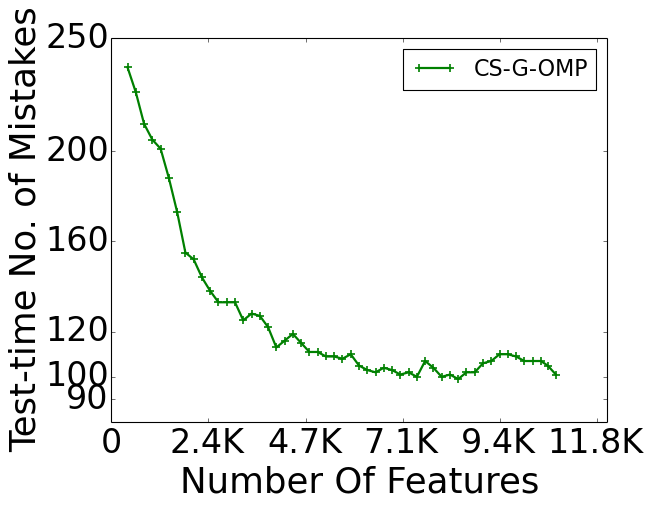
\includegraphics[width=0.3\textwidth]{img/extra_exp_v2.png}
\caption{CS-G-OMP test-time performance on MNIST} 
\label{fig:mnist}
\end{figure}
We present here experimental results of CS-G-OMP with generalized linear models on a MNIST database of handwritten digit classification\cite{MNIST}.
We generate features from raw digit pixels following the recent development of \cite{gem}. It  generates about 11,000 dimensional features via generalized eigenvectors of pairs of second moments of the raw pixel values of different classes, and achieves one-percent error rate with logistic regressions. We partition the generated features into 54 equal-sized random feature groups, and apply CS-G-OMP with multi-class-logistic regression, targeting the one-hot encodings of sample labels. Mathematically, we choose our mean function of generalized linear model, $\nabla \phi: \mathbb{R}^P \rightarrow \mathbb{R}^P$, as $\nabla \phi(x) = \frac{exp(x)}{\sum _p^P exp(x)_p}$ for Algorithm~\ref{algo:gomp_glm}, where $exp(x)$ is an element-wise exponential function. 

As shown in Figure~\ref{fig:mnist}, the test-time accuracy improves greatly at start, quickly reducing the number of mistakes below 150 (i.e., 98.5\% accuracy with the 10K test samples of MNIST) with 2200 out of the 11k total features, and plateaus between 105 and 100 mistakes with 6k features and beyond. The peak performance is 99 mistakes, and the final result has 101 mistakes. We were unable to reproduce results of \cite{gem}, which has 96 mistakes, possibly because of feature generation parameter tuning. Since logistic regression with 11K features and 60K training samples takes non-trivial time to train, the runtime gap between CS-G-OMP and CS-G-FR further widens: CS-G-OMP is able to finish the sequencing in 12 hours, while CS-G-FR takes days to progress. This is because the model training time is orders of magnitudes longer than that of computing gradient w.r.t. the coefficient matrix. In fact, one selection of CS-G-FR takes longer than the full run of CS-G-OMP. As a result, we do not report CS-G-FR result on this data-set.






%\bibliographystyle{plainnat}
%\bibliography{final}
%\end{document}


\chapter{Anytime Neural Network via Adaptive Loss Balancing}
\label{chapter:ann}
%\def\year{2019}\relax
%\documentclass[letterpaper]{article}
%\usepackage{aaai19}
%\usepackage{times}
%\usepackage{helvet}
%\usepackage{courier}
%\usepackage{url}
%\usepackage{graphicx}
%\frenchspacing 
%\setlength{\pdfpagewidth}{8.5in}
%\setlength{\pdfpageheight}{11in}
%\setcounter{secnumdepth}{2} 
%
%%PDF Info Is Required:
%  \pdfinfo{
%/Title (Learning Anytime Predictions in Neural Networks via Adaptive Loss Balancing)
%/Author (Hanzhang Hu, Debadeepta Dey, Martial Hebert, J. Andrew Bagnell)}
%
%\usepackage{subfig}
%\usepackage{xspace}
%\usepackage{color}
%\usepackage{longtable}
%\usepackage{hhline}
%
%% For algorithms
%\usepackage{algorithm}
%\usepackage{algorithmic}
%
%
%% Employ the following version of the ``usepackage'' statement for
%% submitting the draft version of the paper for review.  This will set
%% the note in the first column to ``Under review.  Do not distribute.''
%
%%\usepackage{fancyhdr}		% allows headers and footers
%%\usepackage{lastpage}		% provides page number of last page
%
%\usepackage{amsmath}
%\usepackage{amssymb}
%\usepackage{amsthm}
%
%\makeatletter
%\newtheorem*{rep@theorem}{\rep@title}
%\newcommand{\newreptheorem}[2]{%
%\newenvironment{rep#1}[1]{%
% \def\rep@title{#2 \ref{##1}}%
% \begin{rep@theorem}}%
% {\end{rep@theorem}}}
%\makeatother
%
%\newreptheorem{theorem}{Theorem}
%\newreptheorem{definition}{Definition}
%
%
%\newtheorem{theorem}{Theorem}[section]
%\newtheorem{lemma}[theorem]{Lemma}
%\newtheorem{proposition}[theorem]{Proposition}
%\newtheorem{corollary}[theorem]{Corollary}
%\newtheorem{definition}[theorem]{Definition}
%\newtheorem{assumption}[theorem]{Assumption}
%\newenvironment{myproof}[1][\proofname]{\proof[#1]\mbox{}}{\endproof}
%
%\newcommand{\annnames}{Anytime Neural Networks\xspace}
%\newcommand{\annname}{Anytime Neural Network\xspace}
%\newcommand{\ann}{ANN\xspace}
%\newcommand{\annnp}{ANN} 
%\newcommand{\anns}{ANNs\xspace}
%\newcommand{\aannnp}{AANN}
%\newcommand{\aann}{AANN\xspace}
%\newcommand{\aanns}{AANNs\xspace}
%\newcommand{\adaloss}{AdaLoss\xspace}
%\newcommand{\sieve}{SIEVE\xspace}
%\newcommand{\explin}{EXP-LIN\xspace}
%\newcommand{\const}{CONST\xspace}
%\newcommand{\linear}{LINEAR\xspace}
%\newcommand{\round}[1]{\lfloor #1 \rceil}
%
%\title{Learning Anytime Predictions in Neural Networks  
%via Adaptive Loss Balancing  }
%
%\author{
%Hanzhang Hu,\textsuperscript{\rm 1}
%Debadeepta Dey,\textsuperscript{\rm 2}
%Martial Hebert,\textsuperscript{\rm 1}
%J. Andrew Bagnell\textsuperscript{\rm 1}\\
%\textsuperscript{\rm 1}Carnegie Mellon University,
%\textsuperscript{\rm 2}Microsoft Research\\
%hanzhang@cs.cmu.edu, dedey@microsoft.com, hebert@cs.cmu.edu, dbagnell@cs.cmu.edu
%}
%
%
%\begin{document}
%\maketitle
%\begin{abstract}
%This work considers the trade-off between accuracy and test-time computational cost of deep neural networks (DNNs) via \emph{anytime} predictions from auxiliary predictions. Specifically, we optimize auxiliary losses jointly in an \emph{adaptive} weighted sum, where the weights are inversely proportional to average of each loss. 
%Intuitively, this balances the losses to have the same scale.
%We demonstrate theoretical considerations that motivate this approach from multiple viewpoints, including connecting it to optimizing the geometric mean of the expectation of each loss, an objective that ignores the scale of losses. 
%Experimentally, the adaptive weights induce more competitive anytime predictions on multiple recognition data-sets and models than non-adaptive approaches including weighing all losses equally. In particular, anytime neural networks (\anns) can achieve the same accuracy faster using adaptive weights on a small network than using static constant weights on a large one.
%For problems with high performance saturation, we also show a sequence of exponentially deepening \anns can achieve near-optimal anytime results at any budget, at the cost of a const fraction of extra computation. 
%\end{abstract}
%
%

\section{Introduction}
\label{sec:introduction}

Recent years have seen advancement in visual recognition tasks
by increasingly accurate convolutional neural networks, from AlexNet~\cite{alexnet} and VGG~\cite{vgg}, to ResNet~\cite{resnet}, ResNeXt~\cite{resnext}, and DenseNet~\cite{densenet}. 
As models become more accurate and computationally expensive, it becomes more difficult for applications to choose between slow predictors with high accuracy and fast predictors with low accuracy. 
Some applications also desire multiple trade-offs between computation and accuracy, because they have computational budgets that may vary at test time. E.g., web servers for facial recognition or spam filtering may have higher load during the afternoon than at midnight.  Autonomous vehicles need faster object detection when moving rapidly than when it is stationary.  Furthermore, real-time and latency sensitive applications may desire fast predictions on easy samples and slow but accurate predictions on difficult ones. 
\begin{figure}
    \centering
    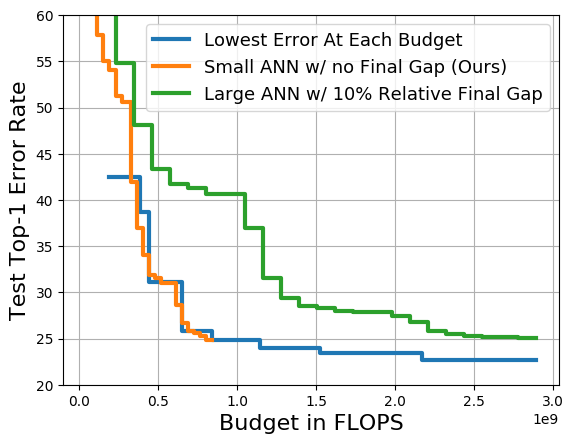
\includegraphics[width=0.85\linewidth, keepaspectratio]{\ANNDIR/adaloss_small_vs_const_large.png}
    \caption{The common \ann training strategy increases final errors from the optimal (green vs. blue), which decreases exponentially slowly. By learning to focus more on the final auxiliary losses, the proposed adaptive loss weights make a small \ann (orange) to outperform a large one (green) that has non-adaptive weights. }
    \label{fig:sieve_small_vs_const_large}
\end{figure}

An \textbf{anytime predictor}~\cite{horvitz:1987,boddydean,anytime,speedboost,msdense} can automatically trade off between computation and accuracy. For each test sample, an anytime predictor produces a fast and crude initial prediction and continues to refine it as budget allows, so that at any test-time budget, the anytime predictor has a valid result for the sample, and the more budget is spent, the better the prediction. 
Anytime predictors are different from cascaded predictors~\cite{cascade,xu:14,cai:15,adaptivenn,cascade_nn} for \textbf{budgeted prediction}, which aim to minimize \textbf{average test-time computational cost} without sacrificing average accuracy: a different task (with relation to anytime prediction). Cascades achieve this by early exiting on easy samples to save computation for difficult ones, but cascades cannot incrementally improve individual samples after an exit. Furthermore, early exit policy of cascades can be combined with existing anytime predictors~\cite{adaptivenn,cascade_nn}. Hence, we consider cascades to be orthogonal to anytime predictions.




\begin{figure}
    \centering
    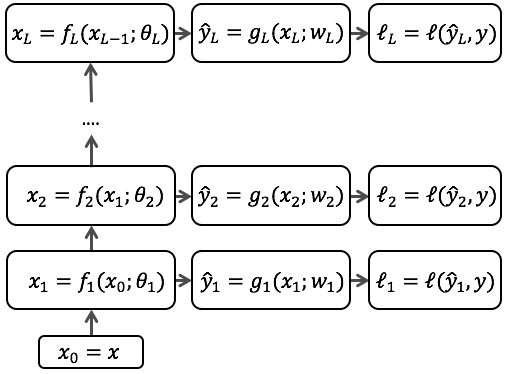
\includegraphics[width=0.85\linewidth, keepaspectratio]{\ANNDIR/ann.png}
    \caption{Anytime neural networks contain auxiliary predictions and losses, $\hat{y}_i$ and $\ell_i$, for intermediate feature unit $f_i$.  }
    \label{fig:ann}
\end{figure}

This work studies how to convert well-known DNN architectures to produce competitive anytime predictions.  
We form anytime neural networks (\anns) by appending auxiliary predictions and losses to DNNs, as we will detail in Sec.~\ref{sec:ann} and Fig.~\ref{fig:ann}. Inference-time prediction then can be stopped at the latest prediction layer that is within the budget. Note that this work deals with the case where it is \textbf{not known apriori} where the interrupt during inference time will occur. 
We define the optimal at each auxiliary loss as the result from training the \ann only for that loss to convergence. Then our objective is to have near-optimal final predictions and competitive early ones.  Near-optimal final accuracy is imperative for anytime predictors, because, as demonstrated in Fig.~\ref{fig:sieve_small_vs_const_large}, accuracy gains are often exponentially more expensive as model sizes grow, so that reducing 1\% error rate could take 50\% extra computation. Unfortunately, existing anytime predictors often optimize the anytime losses in static weighted sums~\cite{supervisednet,feedbacknet,msdense} that poorly optimize final predictions, as we will show in Sec.~\ref{sec:multi_objective} and Sec.~\ref{sec:experiment_questions}.

Instead, we optimize the losses in an \textbf{adaptive} weighted sum, where the weight of a loss is inversely proportional to the empirical mean of the loss on the training set. Intuitively, this normalizes losses to have the same scale, so that the optimization leads each loss to be about the same relative to its optimal. We provide multiple theoretical considerations to motivate such weights.
First of all, when the losses are mean square errors, our approach is maximizing the likelihood of a model where the prediction targets have Gaussian noises. Secondly, inspired by the maximum likelihood estimation, we optimize the model parameters and the loss weights jointly, with log-barriers on the weights to avoid the trivial solution of zero weights. Finally, we find the joint optimization equivalent to optimizing the geometric mean of the expected training losses, an objective that treats the relative improvement of each loss equally. Empirically, we show on multiple models and visual recognition data-sets that the proposed adaptive weights outperform natural, non-adaptive weighting schemes as follows.
We compare small \anns using our adaptive weights against \anns that are $50\sim 100\%$ larger but use non-adaptive weights. The small \anns can reach the same final accuracy as the larger ones, and reach each accuracy level faster.

Early and late accuracy in an \ann are often anti-correlated (e.g., Fig.~7 in~\cite{msdense} shows \anns with better final predictions have worse early ones). To mitigate this \emph{fundamental} issue we propose to assemble \anns of exponentially increasing depths. If \anns are near-optimal in a late fraction of their layers, the exponential ensemble only pays a constant fraction of additional computation to be near-optimal at every test-time budget. In addition, exponential ensembles outperform linear ensembles of networks, which are commonly used baselines for existing works~\cite{feedbacknet,msdense}. 
In summary our contributions are:
\begin{itemize}
    %\item We highlight the importance of near-optimal final predictions in anytime models.
    \item We derive an adaptive weight scheme for training losses in \anns from multiple theoretical considerations, and show that experimentally this scheme achieves near-optimal final accuracy \emph{and} competitive anytime ones on multiple data-sets and models.
    \item We assemble \anns of exponentially increasing depths to achieve near-optimal anytime predictions at every budget at the cost of a constant fraction of additional consumed budget. 
\end{itemize}



\section{Related Works}
\label{sec:background}


\textbf{Meta-algorithms for anytime and budgeted prediction.}
Anytime and budgeted prediction has a rich history in learning literature.
\cite{weinberger09feature,xu:12,xu:13b} sequentially generate features to empower the final predictor.
\cite{reyzin:11,speedboost,hu:16} apply boosting and greedy methods to order feature and predictor computation.  
\cite{timeliness,rl_anytime} form Markov Decision Processes for computation of weak predictors and features, and learn policies to order them. However, these meta-algorithms are not easily compatible with complex and accurate predictors like DNNs, because the anytime predictions without DNNs are inaccurate, and there are no intermediate results during the computation of the DNNs.
Cascade designs for budgeted prediction \cite{cascade,lefakis:10,chen:12,xu:14,cai:15,adaptive_select,adaptivenn,cascade_nn} reduce the average test-time computation by early exiting on easy samples and saving computation for difficult ones. As cascades build upon existing anytime predictors, or combine multiple predictors, they are orthogonal to learning \anns end-to-end.

\textbf{Neural networks with early auxiliary predictions.} 
Multiple works have addressed training DNNs with early auxiliary predictions for various purposes. \cite{supervisednet,inception_v4,pspnet,fractalnet} use them to regularize the networks for faster and better convergence. \cite{curriculum,feedbacknet} set the auxiliary predictions from easy to hard for curriculum learning. \cite{hed,reverse_scene_seg} make pixel level predictions in images, and find learning early predictions in coarse scales also improve the fine resolution predictions. \cite{msdense} shows the crucial importance of maintaining multi-scale features for high quality early classifications. The above works use manually-tuned static weights to combine the auxiliary losses, or change the weights only once~\cite{reverse_scene_seg}. This work proposes adaptive weights to balance the losses to the same scales online, and provides multiple theoretical motivations. We empirically show adaptive losses induce better \anns on multiple models, including the state-of-the-art anytime predictor for image recognition, MSDNet~\cite{msdense}. %There also exist works that train auxiliary losses stage-wise~\cite{boostresnet}, but they suffer from worse accuracy generally. 

\textbf{Model compression.} 
Many  works have studied how to compress neural networks.  \cite{prune_nn,slim_nn} prune network weights and connections. \cite{binary_nn,binary_nn_eccv,squeezenet} quantize weights within networks to reduce computation and memory footprint. 
\cite{wang2017skipnet,veit2017convolutional} dynamically skip network computation based on samples.
\cite{deepreally,distillation} transfer knowledge of deep networks into shallow ones by changing the training target of shallow networks. 
These works are orthogonal to ours, because they train a separate model for each trade-off between computation and accuracy, but we train a single model to handle all possible trade-offs.



%#########################################################
%               Methods
%#########################################################

\section{Optimizing Anytime Predictors}

%\subsection{Training Anytime Neural Networks via Multi-objective Optimization}
\label{sec:ann}

%\subsection{Anytime Augmentation to a Feed-forward Network}
%\label{sec:ann-struct}




%given a sample $(x,y)\sim D$, the initial feature map $x_0$ is set to $x$, and the subsequent feature transformations $f_1, f_2,..., f_L$ generate a sequence of intermediate features $x_i = f_i(x_{i-1} ; \theta_i)$ for $i\geq 1$ using parameter $\theta_i$.  Each feature map $x_i$ can then produce an auxiliary prediction $\hat{y}_i$ using a prediction layer $g_i$: $\hat{y}_i = g_i(x_i; w_i)$ with parameter $w_i$. Each auxiliary prediction $\hat{y}_i$ then incurs an expected loss $\ell_i := E _{(x,y) \sim D} [ \ell( y, \hat{y}_i)]$. We call such an augmented network as an \textit{\annname (\ann)}. 


%For instance, if we base ANNs on ResNets \cite{resnet}, then each $f_i$ contains $s$ number of residual building blocks (whose implementation details are deferred to the appendix), where $s$ is the prediction period. Each $g_i$ outputs the predicted label distribution $\hat{y}_i$ using a global pooling layer followed by a linear layer and a softmax; the loss function $\ell$ is the cross-entropy loss.
%During test-time, an \ann computes $\hat{y}_i$ sequentially until interruption from either users or early exit policies. %The above augmentation is general to feed-forward convolutional network as we experiment in Sec.~\ref{sec:other_networks}.  



%since complex neural networks can fit any labeling of the data for our available data-sets \cite{bengio2016}, 
%when the network is highly over-parameterized, it may be reasonable to assume that the sub neural networks of the full network can encode extra information to enable competitive early predictions, and there may exist $\theta$ such that $\ell_i (\theta) \approx \ell_i^*$ for any $i$.  


%Let the parameters of the full \ann be $\theta = (\theta_1, w_1,  ..., \theta_L, w_L)$. Let $\ell^*_i := \min _{\theta} \ell_i(\theta)$ be the optimal loss at the $i^{th}$  prediction. The goal of training an \ann is to find a single $\theta^*$ such that $\ell_i(\theta^*) =\ell^*_i$ for all $i$, i.e., 
%$ \theta^* \in \cap _{i=1}^L \{ x : x = \arg \min _{\theta} \ell _i(\theta) \}. \label{eq:multi-objective}$
% If the above multi-objective optimization can be solved, then there exists a $\theta^*$ such that simultaneously optimizes all $\ell_i$, i.e., $\ell_i(\theta^*) = \ell_i^*$ for any $i$. 


\label{sec:multi_objective}

As illustrated in Fig.~\ref{fig:ann}, a feed-forward network consists of a sequence of transformations $f_1,...,f_L$ of feature maps. Starting with the input feature map $x_0$, each subsequent feature map is generated by $x_i = f_i(x_{i-1})$.  Typical DNNs use the final feature map $x_L$ to produce predictions, and hence require the completion of the whole network for results. Anytime neural networks (\anns) instead introduce auxiliary predictions and losses using the intermediate feature maps $x_1,...,x_{L-1}$, and thus, have early predictions that are improving with computation. 


%%%%%%%%%%%%%%%%%


\textbf{Weighted sum objective.} Let the intermediate predictions be $\hat{y}_i = g_i(x_i)$ for some function $g_i$, and let the corresponding expected loss be $\ell_i = E_{(x_0,y)\sim \mathcal{D}} [\ell(y, \hat{y}_i)]$, where $\mathcal{D}$ is the distribution of the data, and $\ell$ is some loss such as cross-entropy.  Let $\theta$ be the parameter of the \ann, and define the optimal loss at prediction $\hat{y}_i$ to be $\ell_i* = \min _{\theta}  \ell_i(\theta)$. Then the goal of anytime prediction is to seek a universal 
$
    \theta^* \in \cap _{i=1}^L \{ \theta' : \theta' = \arg \min _{\theta} \ell _i(\theta) \}.
    \label{eq:multi-objective}
$
Such an ideal $\theta^*$ does not exist in general as this is a multi-objective optimization, which only has Pareto front, a set containing all solutions such that improving one $\ell_i$ necessitates degrading others. Finding all solutions in the Pareto front for \anns is not practical or useful, since this requires training multiple models, but each \ann only runs one. Hence, following previous works on anytime models~\cite{supervisednet,feedbacknet,msdense}, we optimize the losses in a weighted sum
$
    \min _{\theta} \sum _{i=1}^L B_i \ell_i (\theta),
    \label{eq:sum-objective}
$
where $B_i$ is the weight of the loss $\ell_i$. We call the choices of $B_i$ \textit{weight schemes}. 


%%%%%%%%%%%%%%%%%

\textbf{Static weight schemes.} Previous works often use static weight schemes as part of their formulation. \cite{supervisednet,hed,msdense} use \const scheme that sets $B_i =1$ for all $i$. \cite{feedbacknet} use \linear scheme that sets $B_1$ to $B_L$ to linearly increase from $0.25$ to $1$. However, as we will show in Sec.~\ref{sec:compare_opt}, these static schemes not only cannot adjust weights in a data and model-dependent manner, but also may significantly degrade predictions at later layers.

\begin{figure}
    \centering
        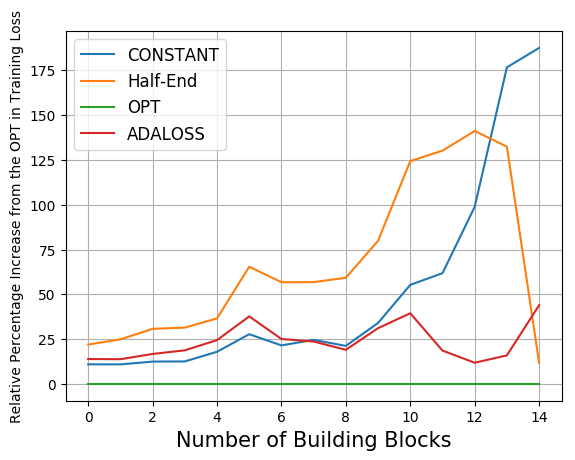
\includegraphics[width=0.80\linewidth, keepaspectratio]{\ANNDIR/loss_cifar100.png}
    \caption{Relative Percentage Increase in Training Loss vs. depths (lower is better). \const scheme is increasingly worse than the optimal at deep layers. \adaloss performs about equally well on all layers in comparison to the OPT.}
    \label{fig:loss_cifar100}
\end{figure}

\begin{figure}
    \centering
    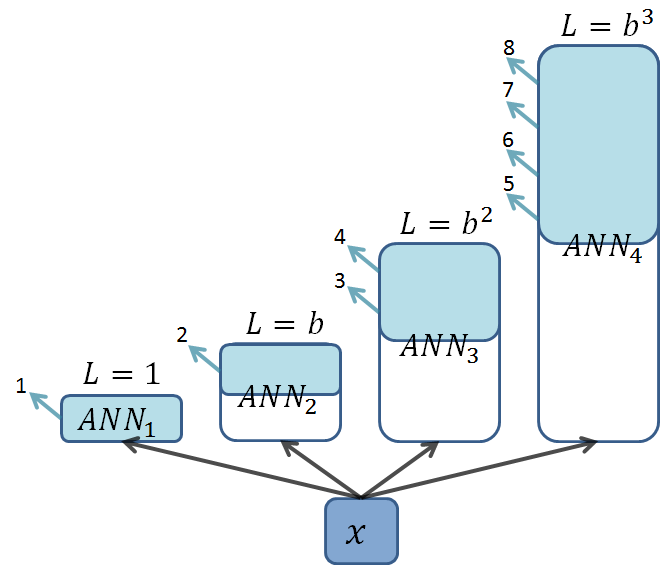
\includegraphics[width=0.75\linewidth, keepaspectratio]{\ANNDIR/EANN.png}
    \caption{ Ensemble of exponentially deepening anytime neural network (EANN) computes its \anns in order of their depths. An anytime result is used if it is better than all previous ones on a validation set (layers in light blue).} 
     \label{fig:eann}
\end{figure}
    %}    
    
%%%%%%%%%%%%%%


\textbf{Qualitative weight scheme comparison.} Before we formally introduce our proposed adaptive weights, we first shed light on how existing static weights suffer. We experiment with a ResNet of 15 basic residual blocks on CIFAR100~\cite{cifar} data-set (See Sec.~\ref{sec:experiment_questions} for data-set details). An anytime predictor is attached to each residual block, and we estimate the optimal performance (OPT) in training cross entropy of predictor $i$ by training a network that has weight only on $\ell_i$ to convergence. Then for each weight scheme we train an \ann to measure the relative increase in training loss at each depth $i$ from the OPT. In Fig.~\ref{fig:loss_cifar100}, we observe that the intuitive \const scheme has high relative losses in late layers. This indicates that there is not enough weights in the late layers, though losses have the same $B_i$.  We also note that balancing the weights is non-trivial. For instance, if we put half of the total weights in the final layer and distribute the other half evenly, we get the ``Half-End" scheme. As expected, the final loss is improved, but this is at the cost of significant increases of early training losses. In contrast, the adaptive weight scheme that we propose next (\adaloss), achieves roughly even relative increases in training losses automatically, and is much better than the \const scheme in the late layers.

%%%%%%%%%%%%%%

\textbf{Adaptive Loss Balancing (\adaloss).} 
% Why the auxiliary losses should have different weights when they are all cross-entropy losses between predictions and the target label? 
Given all losses are of the same form (cross-entropy), it may be surprising
that better performance is achieved with differing weights.
Because early features typically have less predictive power than later ones, early losses are naturally on a larger scale and possess larger gradients. Hence, if we weigh losses equally, early losses and gradients often dominate later ones, and the optimization becomes focused on the early losses.  
To automatically balance the weights among the losses of different scales, we propose an adaptive loss balancing scheme (\adaloss). Specifically, we keep an exponential average of each loss $\hat{\ell}_i$ during training, and set $B_i \propto  \frac{1}{\hat{\ell}_i}$. This is inspired by \cite{reverse_scene_seg}, which scales the losses to the same scale \emph{only once} during training, and provides a brief intuitive argument: the adaptive weights set the losses to be on the same scale. 
We next present multiple theoretical justifications for \adaloss.
 
Before considering general cases, we first consider a simple example, where the loss function $\ell(y, \hat{y}) = \Vert y - \hat{y}\Vert^2_2$ is the square loss. For this example, we model each $y|x$ to be sampled from the multiplication of $L$ independent Gaussian distributions, $\mathcal{N}(\hat{y}_i, \sigma_i^2 I)$ for $i=1,...,L$, where $\hat{y}_i(x; \theta)$ is the $i^{th}$ prediction, and $\sigma_i^2 \in \mathbb{R}^+$, i.e., 
$Pr(y|x ; \theta, \sigma_1^2,..., \sigma_L^2) \propto \prod _{i=1}^L  \frac{1}{\sqrt{\sigma_i^2}}\exp(-\frac{\Vert y - \hat{y}_i\Vert_2^2 }{2 \sigma_i^2})$. 
Then we compute the empirical expected log-likelihood for a maximum likelihood estimator (MLE):
\begin{align}
\hat{E}\big[\ln (Pr(y|x))\big]
&\propto  \hat{E} \big[\sum _{i=1}^L( -\frac{\Vert y - \hat{y}_i\Vert^2_2}{\sigma_i^2} -  \ln \sigma_i^2 ) \big] \\
&= \sum _{i=1}^L ( -\frac{\tilde{\ell}_i }{\sigma_i^2} -  \ln \sigma_i^2 ),
\label{eq:mle_to_log_barrier}
\end{align}
where $\hat{E}$ is averaging over samples, and $\tilde{\ell}_i$ is the empirical estimate of $\ell_i$. If we fix $\theta$ and optimize over $\sigma_i^2$, we get $\sigma_i^2 = \tilde{\ell}_i$.
As computing the empirical means is expensive over large data-sets, \adaloss replaces $\tilde{\ell}_i$ with $\hat{\ell}_i$, the exponential moving average of the losses, and sets $B_i \propto \hat{\ell}_i^{-1} \approx \sigma_i^{-2}$ so as to solve the MLE online by jointly updating $\theta$ and $B_i$. We note that the naturally appeared $\ln \sigma_i^2$ terms in Eq.~\ref{eq:mle_to_log_barrier} are log-barriers preventing $B_i=0$. 

Inspired by this observation, we form the following joint optimization over $\theta$ and $B_i$ for general losses without probability models:
\begin{align}
    \min _{\theta, B_1,...,B_L} \sum _{i=1}^L (B_i \ell _i(\theta) - \lambda \ln B_i),
    \label{eq:weighted_sum_log_barrier}
\end{align}
where $\lambda > 0$ is a hyper parameter to balance between the log-barriers and weighted losses. Under the optimal condition, $B_i=\frac{\lambda}{\ell_i}$. \adaloss estimates this with $B_i \propto \hat{\ell}_i(\theta)^{-1}$.  
We can also eliminate $B_i$ from Eq.~\ref{eq:weighted_sum_log_barrier} under the optimal condition, and we transform Eq.~\ref{eq:weighted_sum_log_barrier} to the following problem:
\begin{align}
    \min _{\theta} \sum _{i=1}^L \ln \ell _i (\theta).
    \label{eq:geometric_mean}
\end{align}
This is equivalent to minimizing the geometric mean of the expected training losses, and it differs from minimizing the expected geometric mean of losses, as $\ln$ and expectation are not commutable. 
Eq.~\ref{eq:geometric_mean} discards any constant scaling of losses automatically discarded as constant offsets, so that the scale difference between the early and late losses are automatically reconciled. Geometric mean is also known as the canonical mean for multiple positive quantities of various scales. \adaloss optimizes  Eq.~\ref{eq:geometric_mean}, since the objective gradient is $\sum _{i=1}^L \frac{ \nabla \ell _i (\theta)} {\ell_i (\theta)}$. \adaloss wants to weigh each $\ell_i(\theta)$ by exactly $\frac{1}{{\ell}_i (\theta) }$, and estimates the weight by $\frac{1}{\hat {\ell}_i (\theta) }$.
This concludes our theoretical considerations for \adaloss.



%%%%%%%%%%%%%%%%




\section{Sequence of Exponentially Deepening Anytime Neural Networks (EANN)}
\label{sec:eann}


In practice, we often observe \anns using \adaloss to be much more competitive in their later half than the early half on validation sets, such as in Table.~\ref{tab:compare_f} of Sec.~\ref{sec:compare_opt}. Fortunately, we can leverage this effect to form competitive anytime predictors at every budget, with a constant fraction of additional computation. Specifically, we assemble \anns whose depths grow exponentially. Each \ann only starts computing if the smaller ones are finished, and its predictions are used if they are better than the best existing ones in validation. We call this ensemble an \textbf{EANN}, as illustrated in Fig.~\ref{fig:eann}. An EANN only delays the computation of any large \ann by at most a constant fraction of computation, because the earlier networks are exponentially smaller. Hence, if each \ann is near-optimal in later predictions, then we can achieve near-optimal accuracy at any test-time interruption, with the extra computation. 
Formally, the following proposition characterizes the exponential base and the increased computational cost.  


\begin{proposition}
Let $b>1$. Assume for any $L$, any \ann of depth $L$ has competitive anytime prediction at  depth $i > \frac{L}{b}$ against the optimal of depth $i$. Then after $B$ layers of computation, EANN produces anytime predictions that are competitive against the optimal of depth $\frac{B}{C}$ for some $C > 1$, such that $\sup _B C = 2+ \frac{1}{b-1}$, and $C$ has expectation
$E_{B\sim uniform(1,L)}[C] \leq 1 - \frac{1}{2b} + \frac{1 + \ln (b)}{b-1}$.
\label{prop:eann}
\end{proposition}
This proposition says that an EANN is competitive at any budget $B$ against the optimal of the cost $\frac{B}{C}$. Furthermore, the stronger each anytime model is, i.e., the larger $b$ becomes, the smaller the computation inflation, $C$, is: as $b$ approaches $\infty$, $\sup  _B C$, shrinks to 2, and $E[C]$, shrinks to 1.
Moreover, if we have $M$ number of parallel workers instead of one, we can speed up EANNs by computing \anns in parallel in a first-in-first-out schedule, so that we effectively increase the constant $b$ to $b^M$ for computing $C$. It is also worth noting that if we form the sequence using regular networks instead of \anns, then we will lose the ability to output frequently, since at budget $B$, we only produce $\Theta(\log(B))$ intermediate predictions instead of the $\Theta(B)$ predictions in an EANN. We will further have a larger cost inflation, $C$, such that $\sup  _B C \geq 4$ and $E[C] \geq 1.5 + \sqrt{2} \approx 2.91$, so that the average cost inflation is at least about $2.91$.
We defer the proofs to the appendix.




%#############################  ############################
%               EXPERIMENTS
%#############################  ############################
\section{Experiments}
\label{sec:experiment_questions}

We list the key questions that our experiments aim to answer.
\begin{itemize}

\item How do anytime predictions trained with adaptive weights compare against those trained with static constant weights (over different architectures)?
(Sec.~\ref{sec:compare_opt})
\item How do underlying DNN architectures affect \anns? (Sec.~\ref{sec:compare_opt})
\item How can sub-par early predictions in \anns be mitigated by \ann ensembles? 
(Sec.~\ref{sec:eann_experiment})
\item How does data-set difficulty affect the adaptive weights scheme?
(Sec.~\ref{sec:weight_vs_dataset})
\end{itemize}


\subsection{Data-sets and Training Details}
\label{sec:exp}

\textbf{Data-sets.} We experiment on CIFAR10, CIFAR100~\cite{cifar}, SVHN~\cite{svhn}\footnote{Both CIFAR data-sets consist of 32x32 colored images. CIFAR10 and CIFAR100 have 10 and 100 classes, and each have 50000 training and 10000 testing images. We held out the last 5000 training samples in CIFAR10 and CIFAR100 for validation; the same parameters are then used in other models. We adopt the standard augmentation from \cite{supervisednet,resnet}.
SVHN contains around 600000 training and around 26032 testing 32x32 images of numeric digits from the Google Street Views. We adopt the same pad-and-crop augmentations of CIFAR for SVHN, and also add Gaussian blur.}
and ILSVRC~\cite{ILSVRC15}\footnote{
ILSVRC2012~\cite{ILSVRC15} is a visual recognition data-set containing around 1.2 million natural and 50000 validation images for 1000 classes. We report the top-1 error rates on the validation set using a single-crop of size 224x224, after scaling the smaller side of the image to 256, following~\cite{resnet}.}.

\textbf{Training details.} We optimize the models using stochastic gradient descent, with initial learning rate of 0.1, momentum of 0.9 and a weight decay of 1e-4. On CIFAR and SVHN, we divide the learning rate by 10 at 1/2 and 3/4 of the total epochs. We train for 300 epochs on CIFAR and 60 epochs on SVHN.  On ILSVRC, we train for 90 epochs, and divide the learning rate by 10 at epoch 30 and 60. We evaluate test error using single-crop.


\textbf{Base models.} We compare our proposed \adaloss weights against the intuitive \const weights. On CIFAR and SVHN, we also compare \adaloss against LINEAR and OPT, defined in Sec.~\ref{sec:multi_objective}. 
We evaluate the weights on multiple models including ResNet~\cite{resnet} and DenseNet~\cite{densenet}, and MSDNet~\cite{msdense}. For ResNet and DenseNet, we augment them with auxiliary predictors and losses, and call the resulting models Res\ann and Dense\ann, and defer the details of these models to the appendix Sec.~\ref{sec:implementation_ann}.


\subsection{Weight Scheme Comparisons}
\label{sec:compare_opt}


\begin{table}
    \centering
    \begin{tabular}{c|cccc}
    \hline
     & 1/4 & 1/2 & 3/4 & 1 \\
    \hline
    OPT
	&  0.00 &  0.00 &  0.00 &  0.00 \\
    CONST
	& \textbf{15.07} & 16.40 & 18.76 & 18.90 \\
    LINEAR
	& 25.67 & 13.02 & 12.97 & 12.65 \\
    ADALOSS
 & 32.99 &  \textbf{9.97} &  \textbf{3.96} &  \textbf{2.73} \\
    \hline
    \end{tabular}
        
    \caption{Average relative percentage increase in error from the OPT on CIFAR and SVHN at 1/4, 1/2, 3/4 and 1 of the total cost. E.g., the bottom right entry means that if OPT has a 10\% final error rate, then \adaloss has about 10.27\%.}
    \label{tab:compare_f}
\end{table}

\begin{table}
        \begin{tabular}{c|cccc}
        \hline
         & 1/4 & 1/2 & 3/4 & 1 \\
        \hline
        Res\annnp50+C
    	& \textbf{54.34} & 35.61 & 27.23 & 25.14 \\
        Res\annnp50+A
    	& 54.98 & \textbf{34.92} & \textbf{26.59} & \textbf{24.42} \\
    	\hline
        Dense\annnp169+C  % exp 4007
    	& 48.15 & 45.00 & 29.09 & 25.60 \\
        Dense\annnp169+A % exp 3544
    	& \textbf{47.17} & \textbf{44.64} & \textbf{28.22} & \textbf{24.07} \\
        \hline      
        MSDNet38 
        & \textbf{33.9} & 28.0 & 25.7 & 24.3 \\
        MSDNet38+A % 4113
        & 35.75 & 28.04 & 25.82 & \textbf{23.99} \\
        \hline
        \end{tabular}
        
    
    \caption{ Test error rates at different fraction of the total costs on Res\annnp50, Dense\annnp169, and MSDNet38 on ILSVRC. The post-fix +C and +A stand for \const and \adaloss respectively. Published results of MSDNet38~\cite{msdense} uses \const.
    }
    \label{tab:compare_f_ilsvrc}
\end{table}



\begin{figure*}[t]
    \centering
    
    \subfloat[Res\anns on CIFAR10]{
        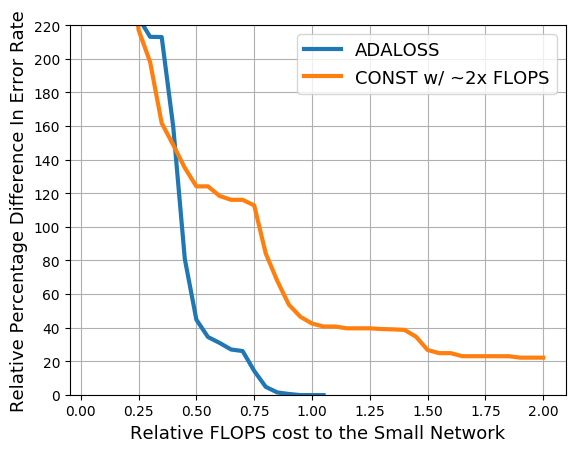
\includegraphics[width=0.32\linewidth, keepaspectratio ]{\ANNDIR/adaloss_vs_const_of_double_cost_cifar10.png}
        \label{fig:adaloss_vs_const_of_double_cost_cifar10}
    }
    ~
    \subfloat[Res\anns on CIFAR100]{
        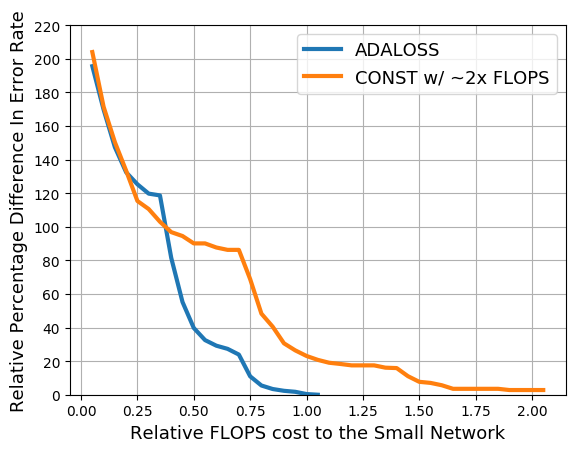
\includegraphics[width=0.32\linewidth, keepaspectratio ]{\ANNDIR/adaloss_vs_const_of_double_cost_cifar100.png}
        \label{fig:adaloss_vs_const_of_double_cost_cifar100}
    }
    ~
    \subfloat[Res\anns on SVHN]{
        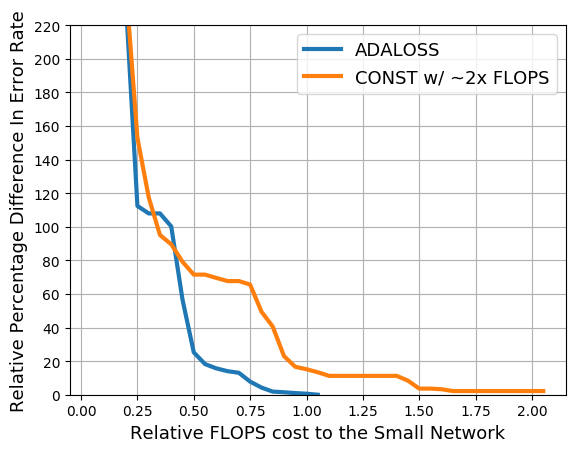
\includegraphics[width=0.32\linewidth, keepaspectratio ]{\ANNDIR/adaloss_vs_const_of_double_cost_svhn.png}
        \label{fig:adaloss_vs_const_of_double_cost_svhn}
    }
    
    \subfloat[Res\anns on ILSVRC]{
        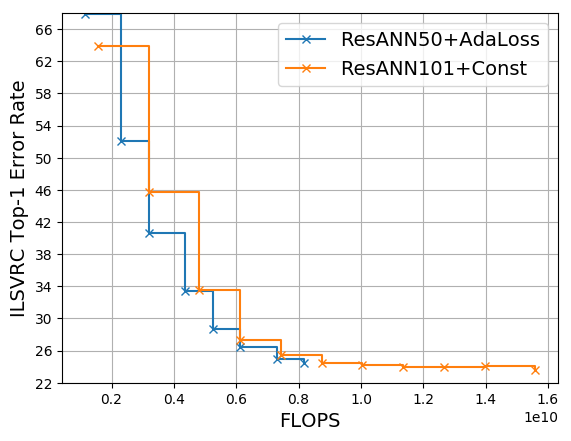
\includegraphics[width=0.32\linewidth, keepaspectratio]{\ANNDIR/ilsvrc_adaloss_vs_const_resnet.png}
        \label{fig:ilsvrc_adaloss_vs_const_of_double_cost}
    }
    ~
    \subfloat[MSDNet on ILSVRC]{
        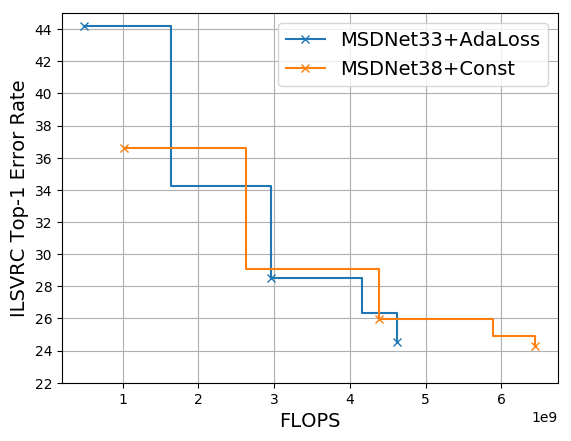
\includegraphics[width=0.32\linewidth, keepaspectratio]{\ANNDIR/ilsvrc_adaloss_vs_const_msdnet.png}
        \label{fig:ilsvrc_adaloss_vs_const_of_double_cost_msdnet}    
    }
    ~
    \subfloat[\anns comparison on ILSVRC]{
        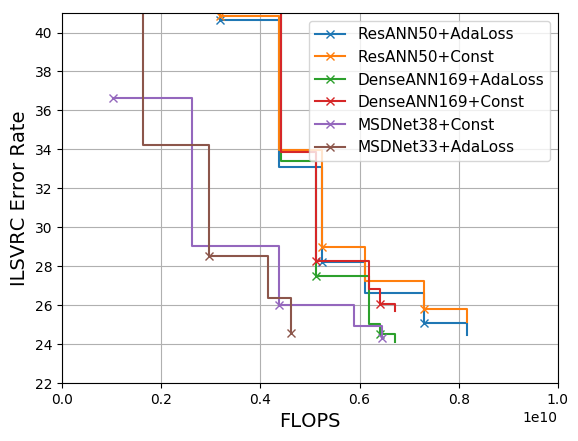
\includegraphics[width=0.32\linewidth, keepaspectratio]{\ANNDIR/ilsvrc_compare_models.png}
        \label{fig:ilsvrc_compare_models}    
    }
    
    \caption{\textbf{(a-e)} Comparing small networks with \adaloss versus big ones using \const. With \adaloss, 
    the small networks achieve the same accuracy levels faster than large networks with \const. 
    \textbf{(f)} \anns performance are mostly decided by underlying models, but \adaloss is beneficial regardless models. }
    \label{fig:adaloss_vs_const_of_double_cost}
\end{figure*}
\textbf{\adaloss vs. \const on the same models.} Table~\ref{tab:compare_f} presents the average relative test error rate increase from OPT on 12  Res\anns on CIFAR10, CIFAR100 and SVHN\footnote{The 12 models are named by $(n,c)$ drawn from $\{ 7, 9, 13, 17, 25 \} \times \{ 16, 32 \}$ and $\{(9,64), (9,128)\}$, where $n$ represents the number of residual units in each of the three blocks of the network, and $c$ is the filter size of the first convolution.}. As training an OPT for each depth is too expensive, we instead report the average relative comparison at 1/4, 1/2, 3/4, and 1 of the total \ann costs. 
We observe that the \const scheme makes $15\sim 18\%$ more errors than the OPT, and the relative gap widens at later layers.  The \linear scheme also has about 13\% relative gap in later layers. In contrast, \adaloss enjoys small performance gaps in the later half of layers. 
On ILSVRC, we compare \adaloss against \const on Res\annnp50, Dense\annnp169, and MSDNet38, which have similar final errors and total computational costs (See Fig.~\ref{fig:ilsvrc_compare_models}). In Table~\ref{tab:compare_f_ilsvrc}, we observe the trade-offs between early and late accuracy on Res\annnp50 and MSDNet38. Furthermore, Dense\annnp169 performs \emph{uniformly} better with \adaloss than with \const. 
Since comparing the weight schemes requires evaluating \anns at multiple budget limits, and \adaloss and \const outperform each other at a significant fraction of depths on most of our experiments, we consider the two schemes \emph{incomparable on the same model}. 
%However, our next experiments will show late predictions to be vastly more important than the early ones.

\begin{figure*}[t]
    \centering
    \subfloat[EANNs on CIFAR100]{
        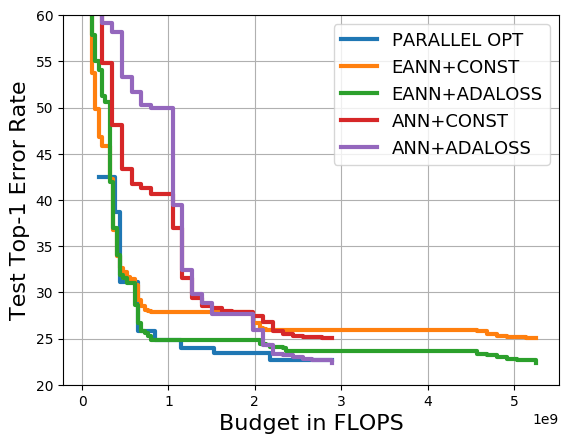
\includegraphics[width=0.32\linewidth, keepaspectratio]{\ANNDIR/cifar100_adaloss_eann_b2.png}
        \label{fig:eann_f}
    }
    ~
    \subfloat[EANN on ILSVRC]{
        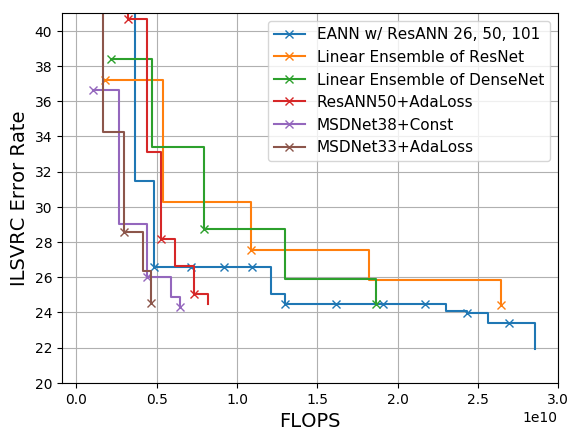
\includegraphics[width=0.32\linewidth, keepaspectratio]{\ANNDIR/eann_comparisons.png}
        \label{fig:compare_ensemble}
    }
    ~
    \subfloat[AdaLoss Weights on three data-sets]{
    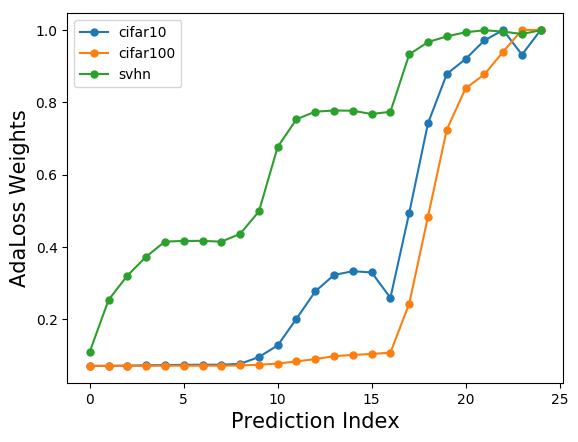
\includegraphics[width=0.32\linewidth, keepaspectratio]{\ANNDIR/adaloss_weights.png}
    \label{fig:adaloss_weights}
    }
    \caption{ \textbf{(a)} EANN performs better if the \anns use \adaloss instead of \const. 
    \textbf{(b)} EANN outperforms linear ensembles of DNNs on ILSVRC.
    \textbf{(c)} The learned adaptive weights of the same model on three data-sets.
    }
    %AANN-14 finishes at 33.50\% error,
\end{figure*}


\textbf{Small networks with \adaloss vs. large ones with \const.} 
Our previous comparison between \adaloss and \const on the same models is not fully conclusive, since each scheme can outperform the other at a significant portion of the total cost. To address this, we set the final error rate, model architecture type, and the filter size $c$ as constants, and vary the model depths so that \adaloss and \const reach the target final error rate. Then we compare the early predictions and the costs of models. 
On each of CIFAR10, 100 and SVHN, we compare six pairs of Res\anns, where the \const uses twice the computation as \adaloss\footnote{\adaloss takes $(n,c)$ from $\{7,9,13\} \times \{16, 32\}$, and \const takes $(n,c)$ from $\{13,17,25\} \times \{16, 32\}$.}. Fig.~\ref{fig:adaloss_vs_const_of_double_cost_cifar10},~\ref{fig:adaloss_vs_const_of_double_cost_cifar100}, and~\ref{fig:adaloss_vs_const_of_double_cost_svhn} show the averaged relative comparisons\footnote{The relative plots pivot at the final predictor from \adaloss, e.g., the location (0.5, 200) means having half the computation and 200\% extra relative errors than the final predictor from \adaloss}, and they show that the small \anns with \adaloss are better anytime predictors than the large ones with \const, because both models have the same final accuracy (on CIFAR10, the small ones are even better), and the small models reach the same error rates faster than the large ones. We have similar observations on ILSVRC using Res\anns and MSDNets in Fig.~\ref{fig:ilsvrc_adaloss_vs_const_of_double_cost} and Fig.~\ref{fig:ilsvrc_adaloss_vs_const_of_double_cost_msdnet}.
For instance, MSDNet~\cite{msdense} is the state-of-the-art anytime predictor. The published MSDNet38 uses \const, and has 24.3\% error rate using 6.6e9 total FLOPS in convolutions. By switching to \adaloss, we improve a much smaller MSDNet33 (details in the appendix), which costs 4.5e9 FLOPS, to reach 24.5\% final error. The two models also have similar early errors. 

\adaloss can reach the same accuracies with similar or smaller costs than \const, because in practice, a linear decrease in final error rate may often require an exponential increase in total computation, and \const degrades the final performances significantly (Table~\ref{tab:compare_f}). Since \adaloss requires much smaller models than \const to reach the same final errors, and with a fixed final error rate, \adaloss reaches each early error rate with less or similar cost, we conclude that \adaloss is the better scheme for anytime predictions. 

\textbf{Various base networks on ILSVRC.} We compare Res\anns, Dense\anns and MSDNets that have final error rate of near 24\% in Fig.~\ref{fig:ilsvrc_compare_models}, and observe that the anytime performance is mostly decided by the specific underlying model. MSDNets are more cost-effective than Dense\anns, which in turn are better than Res\anns. 
However, \adaloss is helpful regardless of underlying model. Both Res\annnp50 and Dense\annnp169 see improvements switching from \const to \adaloss, which is also shown in Table~\ref{tab:compare_f_ilsvrc}. 
Thanks to \adaloss, Dense\annnp169 achieves the same final error using similar FLOPS as the original published results of MSDNet38~\cite{msdense}. This suggests that~\cite{msdense} improve over Dense\anns by having better early predictions without sacrificing the final cost efficiency via impressive architecture insight. \adaloss brings a complementary improvement to MSDNets, as it enables smaller MSDNets to reach the final error rates of bigger MSDNets, while having similar or better early predictions. 



%%%%%%%%%%%%%%%%%% EANN %%%%%%%%%%%%%%%%%%%%%%%%

\subsection{EANN: Closing Early Performance Gaps by Delaying Final Predictions.}
\label{sec:eann_experiment}



\textbf{EANNs on CIFAR100.} In Fig.~\ref{fig:eann_f}, we assemble Res\anns to form EANNs\footnote{The Res\anns have $c=32$ and $n=7, 13, 25$, so that they form an EANN with an exponential base $b\approx 2$. 
By proposition~\ref{prop:eann}, the average cost inflation is $E[C]\approx 2.44$ for $b=2$, so that the EANN should 
compete against the OPT of $n=20$, using $2.44$ times of original costs.} on CIFAR100 and make three observations.
First, EANNs are better than the \ann in early computation, because the ensembles dedicate early predictions to small networks. Even though \const has the best early predictions as in Table~\ref{tab:compare_f}, it is still better to deploy small networks. 
Second, because the final prediction of each network is kept for a long period, \adaloss leads to significantly better EANNs than \const does, thanks to the superior final predictions from \adaloss. 
Finally, though EANNs delay computation of large networks, it actually appears closer to the OPT, because of accuracy saturation. Hence, EANNs should be considered when performance saturation is severe. 

\textbf{EANN on ILSVRC.}
\cite{msdense} and \cite{feedbacknet} use ensembles of networks of linearly growing sizes as baseline anytime predictors. However, in Fig.~\ref{fig:compare_ensemble}, an EANN using Res\anns of depths 26, 50 and 101 outperforms the linear ensembles of ResNets and DenseNets significantly on ILSVRC.
In particular, this drastically reduces the gap between ensembles and the state-of-the-art anytime predictor MSDNet~\cite{msdense}. 
Comparing Res\ann50 and the EANN, we note that the EANN achieves better early accuracy but delays final predictions. 
As the accuracy is not saturated by Res\ann26, the delay appears significant. Hence, EANNs may not be the best when the performance is not saturated or when the constant fraction of extra cost is critical. 


\subsection{Data-set Difficulty versus Adaptive Weights}
\label{sec:weight_vs_dataset}



In Fig.~\ref{fig:adaloss_weights}, we plot the final \adaloss weights of the same Res\ann model (25,32) on CIFAR10, CIFAR100, and SVHN to study the effects of the data-sets on the weights. We observe that from the easiest data-set, SVHN, to the hardest, CIFAR100, the weights are more concentrated on the final layers. This suggests that \adaloss can automatically decide that harder data-sets need more concentrated final weights to have near-optimal final performance, whereas on easy data-sets, more efforts are directed to early predictions. Hence, \adaloss weights may provide information for practitioners to design and choose models based on data-sets.

\section{Conclusion and Discussion}
This work devises simple adaptive weights, \adaloss, for training anytime predictions in DNNs. We provide multiple theoretical motivations for such weights, and show experimentally that adaptive weights enable small \anns to outperform large \anns with the commonly used non-adaptive constant weights. Future works on adaptive weights includes examining \adaloss for multi-task problems and investigating its ``first-order'' variants that normalize the losses by individual gradient norms to address unknown offsets of losses as well as the unknown scales. We also note that this work can be combined with orthogonal works in early-exit budgeted predictions~\cite{cascade_nn,adaptivenn} for saving average test computation. 


\section*{Acknowledgements} 
This work was conducted in part through collaborative participation in the Robotics Consortium sponsored by the U.S Army Research Laboratory under the Collaborative Technology Alliance Program, Cooperative Agreement W911NF-10-2-0016. 


%%%%%%%%%%%%%%%%%% BIB %%%%%%%%%%%%%%%%%%%%%%%%
%\bibliographystyle{aaai}
%{
%\bibliography{AAAI-HuH.2508}
%}

%%%%%%%%%%%%%%%%%% APPENDIX %%%%%%%%%%%%%%%%%%%%%%%%
%\appendix




\section{Sketch of Proof of Proposition~\ref{prop:eann}}
\begin{proof}
For each budget consumed $x$, we compute the cost $x'$ of the optimal that EANN is competitive against. The goal is then to analyze the ratio $C = \frac{x}{x'}$. 
The first ANN in EANN has depth 1. The optimal and the result of EANN are the same. Now assume EANN is on depth $z$ of ANN number $n+1$ for $n\geq 0$, which has depth $b^{n}$. \\
(Case 1) For $z \leq b^{n-1}$, EANN reuse the result from the end of ANN number $n$. 
The cost spent is $x = z + \sum _{i=0}^{n-1} b^i = z + \frac{b^n-1}{b-1}$. 
The optimal we compete has cost of the last ANN, which is $b^{n-1}$
The ratio satisfies:
\begin{align*} 
C &= x / x' = \frac{z}{b^{n-1}} + 1 + \frac{1}{b-1} - \frac{1}{b^{n-1}(b-1)} \\
&\leq 2 + \frac{1}{b-1} - \frac{1}{b^{n-1}(b-1)} 
< 2+ \frac{1}{b-1}. 
\end{align*}
Furthermore, since $C$ increases with $z$, 
\begin{align*}
&E_{z \sim Uniform(0, b^{n-1})}[C] \\
&\leq b^{1-n} \int _0 ^{b^{n-1}} 
    z b^{1-n}+ 1 + \frac{1}{b-1} \;dz \\
&= 1.5 + \frac{1}{b-1}.
\end{align*}
\\
(Case 2) For $b^{n-1} < z \leq b^n$, EANN outputs anytime results from ANN number $n+1$ at depth $z$. 
The cost is still $x = z +\frac{b^n-1}{b-1}$. The optimal competitor has cost $x' = z$.  Hence the ratio is 
\begin{align*}
C &= x/ x' = 1 + \frac{b^n-1}{z(b-1)} \\
&\leq 2 + \frac{1}{b-1} - \frac{1}{b^{n-1}(b-1)} 
< 2+ \frac{1}{b-1}.
\end{align*}
Furthermore, since $C$ decreases with $z$, 
\begin{align*}
&E_{z \sim Uniform(b^{n-1}, b^n)}[C] \\
& \leq 1 +  
   \frac{1}{b^n - b^{n-1}} \int _{b^{n-1}} ^{b^{n}} 
        \frac{b^n -1}{z(b-1)} \; dz  \\
&= 1 + \frac{(b - b^{1-n}) \ln{b}}{(b-1)^2} \\
&< 1 + \frac{b \ln{b}}{(b-1)^2} 
\end{align*}

Finally, since case 1 and case 2 happen with probability $\frac{1}{b}$ and $(1-\frac{1}{b})$, we have
\begin{align}
    \sup _B C &= 2+ \frac{1}{b-1} \\
\intertext{and}
    E_{B\sim Uniform(0, L)}[C] &\leq 1 - \frac{1}{2b} + \frac{1}{b-1} + \frac{\ln{b}}{b-1}.
\end{align}
We also note that with large $b$, $\sup _B C \rightarrow 2$ and $E[C] \rightarrow 1$ from above.
\end{proof}

If we form a sequence of regular networks that grow exponentially in depth instead of \ann, then the worst case happen right before a new prediction is produced. Hence the ratio between the consumed budget and the cost of the optimal that the current anytime prediction can compete, $C$, right before the number $n+1$ network is completed, is 
\[
    \frac{\sum _{i=1}^n b^i}{b^{n-1}} \xrightarrow[]{n\rightarrow \infty} \frac{b^2}{b-1} = 2 + (b-1) + \frac{1}{b-1} \geq 4. 
\]
Note that $(b-1) + \frac{1}{b-1} \geq 2$ and the inequality is tight at $b=2$. Hence we know $\sup _B {C}$ is at least 4. Furthermore, the expected value of $C$, assume $B$ is uniformly sampled such that the interruption happens on the $(n+1)^{th}$ network, is:
\begin{align*}
    E[C] &= \frac{1}{b^{n}} \int _0 ^{b^{n}} \frac{x + \frac{b^{n}-1}{b-1}}{b^{n-1}} \; dx \\ &\xrightarrow[]{n\rightarrow \infty} 1.5 + \frac{b-1}{2} + \frac{1}{b-1} \geq 1.5 + \sqrt{2} \approx 2.91.
\end{align*}
The inequality is tight at $b = 1 + \sqrt{2}$. With large $n$, since almost all budgets are consumed by the last few networks, we know the overall expectation $E_{B\sim Uniform(0, L)}[C]$ approaches $1.5 + \frac{b-1}{2} + \frac{1}{b-1}$, which is at least $1.5 + \sqrt{2}$.




\section{Implementation Details of \anns}
\label{sec:implementation_ann}


\textbf{CIFAR and SVHN Res\anns.} For CIFAR10, CIFAR100~\cite{cifar}, and SVHN~\cite{svhn}, Res\ann follow \cite{resnet} to have three blocks, each of which has $n$ residual units. Each of such basic residual units consists of two 3x3 convolutions, which are interleaved by BN-ReLU. A pre-activation (BN-ReLU) is applied to the input of the residual units. The result of the second 3x3 conv and the initial input are added together as the output of the unit. The auxiliary predictors each applies a BN-ReLU and a global average pooling on its input feature map, and applies a linear prediction. The auxiliary loss is the cross-entropy loss, treating the linear prediction results as logits. For each $(n,c)$ pair such that $n < 25$, we set the anytime prediction period $s$ to be 1, i.e., every residual block leads to an auxiliary prediction. We set the prediction period $s=3$ for $n=25$. 


\textbf{Res\anns on ILSVRC.} Residual blocks for ILSVRC are bottleneck blocks, which consists of a chain of 1x1 conv, 3x3 conv and 1x1 conv. These convolutions are interleaved by BN-ReLU, and pre-activation BN-ReLU is also applied. Again, the output of the unit is the sum of the input feature map and the result of the final conv. 
Res\annnp50 and 101 are augmented from ResNet50 and 101~\cite{resnet}, where we add BN-ReLU, global pooling and linear prediction to every two bottleneck residual units for ResNet50, and every three for ResNet101. 
We create Res\annnp26 for creating EANN on ILSVRC, and Res\annnp26 has four blocks, each of which has two bottleneck residual units. The prediction period is every two units, using the same linear predictors. 


\textbf{Dense\anns on ILSVRC.} We augment DenseNet169~\cite{densenet} to create Dense\ann169. 
DenseNet169 has 82 dense layers, each of which has a 1x1 conv that project concatenation of previous features to $4k$ channels, where $k$ is the growth rate~\cite{densenet}, followed by a 3x3 conv to generate $k$ channels of features for the dense layer. The two convs are interleaved by BN-ReLU, and a pre-activation BN-ReLU is used for each layer. The 82 layers are organized into four blocks of size 6, 12, 32 and 32. Between each neighboring blocks, a 1x1 conv followed by BN-ReLU-2x2-average-pooling is applied to shrink the existing feature maps by half in the hight, width, and channel dimensions. We add linear anytime predictions every 14 dense layers, starting from layer 12 (1-based indexing). The original DenseNet paper~\cite{densenet} mentioned that they use drop-out with keep rate 0.9 after each conv in CIFAR and SVHN, but we found drop-out to be detrimental to performance on ILSVRC.


\textbf{MSDNet on ILSVRC.} MSDNet38 is described in the appendix of~\cite{msdense}. We set the four blocks to have 10, 9, 10 and 9 layers, and drop the feature maps of the finest resolution after each block as suggest in the original paper. 
We successfully reproduced the published results to 24.3\% error rate on ILSVRC using our Tensorflow implementation. We used the original published results for MSDNet38+\const in the main text. We use MSDNet33, which has four blocks of 8, 8, 8 and 9 layers, for the small network that uses \adaloss. We predict using MSDNet33 every seven layers, starting at the fifth layer (1-based indexing). 



\section{Additional Details of \adaloss}

\label{sec:implementation_adaloss}


\subsection{Weight Regularization} 
In practice, some expected loss $\ell_i$ could be much larger than the other losses, so that \adaloss may assign such $\ell_i$ too small a weight for it to receive enough optimization to recover. To prevent this, we mix the uniform constant weight with \adaloss as a form of regularization as follows in Eq.~\ref{eq:geometric_arithmetic_mean}. Such mixture prevents the weight of $\ell_i$ from being too close to zero. 
\begin{align}
    \min _{\theta} \sum _{i=1}^L \big( \alpha (1 - \gamma) \ln \ell _i (\theta) + \gamma  \ell_i (\theta) \big),
    \label{eq:geometric_arithmetic_mean}
\end{align}
where $\alpha >0$ and $\gamma >0$ are hyper parameters. In practice, since DNNs often have elaborate learning rate schedules that assume $B_L=1$, we choose $\alpha  = \min_i \hat{\ell}_i(\theta)$ at each iteration to scale the max weight to 1. We choose $\gamma = 0.05$ from validation sets on CIFAR10 and CIFAR100 from the set $\{0, 0.05, 0.15\}$.

\subsection{Ablation Study of \adaloss parameters on CIFAR} 


\begin{table}[t]
    \centering
    \begin{tabular}{c|cccc|c}
\hline
$\gamma$ & 1/4 & 1/2 & 3/4 & 1  & sum\\
\hline
0.0
	&  0.00 &  0.00 &  0.00 &  0.00  & 0.00\\
0.05
	& -20.08 & -2.15 &  2.22 &  2.43 & -17.59 \\
0.15
	& -23.88 & -0.20 &  5.18 &  5.17 & -13.72\\
\hline
    \end{tabular}
    \caption{Relative percentage increase in error rate by switching from $\gamma=0$. (lower is better.) A small amount of $\gamma = 0.5$ drastically improves early predictions without increasing late error rate much.}
    \label{tab:adaloss_gamma}
\end{table}


\begin{table}[t]
    \centering
    \begin{tabular}{c|cccc}
\hline
EMA $m$ & 1/4 & 1/2 & 3/4 & 1 \\
\hline
0.9
	&  0.00 &  0.00 &  0.00 &  0.00 \\
0.99
	& -0.29 &  0.25 &  0.05 &  0.15 \\
\hline
    \end{tabular}
    \caption{Relative percentage increase in error rate by switching from $m=0.9$.  (lower is better.) The two options essentially result in the same error rates.}
    \label{tab:adaloss_momentum}
\end{table}

\begin{table}[h!]
    \centering
    \begin{tabular}{c|cccc}
\hline
Update period $e$ & 1/4 & 1/2 & 3/4 & 1 \\
\hline
1
	&  0.00 &  0.00 &  0.00 &  0.00 \\
100
	&  0.71 &  0.23 &  0.24 &  0.45 \\
\hline
    \end{tabular}
    \caption{Relative percentage increase in error rate by switching from $e=0$.  (lower is better.) The options are essentially the same on CIFAR10 and CIFAR100. }
    \label{tab:adaloss_update_per}
\end{table}

We conduct ablation studies for the parameters of \adaloss: (1) $\gamma$ in Eq.~\ref{eq:geometric_arithmetic_mean}, which is the mixture weight of the uniform static weighting, (2) the exponential moving average (EMA) momentum, $m$, for updating the expected loss $\hat{\ell}_i$ at each stochastic gradient descent (SGD) step, and (3) the number of SGD steps $e$ to wait between updating \adaloss weights $B_i$ using the learned $\hat{\ell}_i$. We choose $\gamma \in \{0, 0.05, 0.15 \}$, $m \in \{0.9, 0.99\}$, and $e \in \{1, 100\}$, and evaluate them on CIFAR10 and CIFAR100 ResANNs whose $n \in \{9,17,25\}$ and $c=32$. Over the 72 experiments, we found the effects of $m$, and $e$ are almost negligible, as they generate $<0.5\%$ of relative difference in error rates on average, which translates to $0.1\%$ absolute error difference on CIFAR100. These comparisons are in Table~\ref{tab:adaloss_momentum} and Table~\ref{tab:adaloss_update_per}. In the experiment sections, we choose $m = 0.9$ and $e=1$.

However,  $\gamma$ does affect the performance significantly, as show in Table~\ref{tab:adaloss_gamma}. $\gamma=0$ means pure \adaloss and $\gamma=1$ means \const. We observe that with $\gamma=0.05$, the small amount of uniform static weight reduces the error rate at 1/4 of the total cost by 20\% relatively, but at the cost of minor 2.5\% relative increase in late predictions. Increasing $\gamma$ further to $0.15$ has only marginal benefits to early predictions, but has the same negative impact to late accuracy. This suggests that while a small $\gamma$ helps, we should only use a small amount. Throughout the experiment sections in the main text, we choose $\gamma = 0.05$.




\chapter{Training Gradient Boosting on Stochastic Data Streams}
\label{chapter:sgb}
%% This is file `elsarticle-template-1-num.tex',
%%
%% Copyright 2009 Elsevier Ltd
%%
%% This file is part of the 'Elsarticle Bundle'.
%% ---------------------------------------------
%%
%% It may be distributed under the conditions of the LaTeX Project Public
%% License, either version 1.2 of this license or (at your option) any
%% later version.  The latest version of this license is in
%%    http://www.latex-project.org/lppl.txt
%% and version 1.2 or later is part of all distributions of LaTeX
%% version 1999/12/01 or later.
%%
%% Template article for Elsevier's document class `elsarticle'
%% with numbered style bibliographic references
%%
%% $Id: elsarticle-template-1-num.tex 149 2009-10-08 05:01:15Z rishi $
%% $URL: http://lenova.river-valley.com/svn/elsbst/trunk/elsarticle-template-1-num.tex $
%%
\documentclass[preprint,12pt]{elsarticle}
\frenchspacing 
\setlength{\pdfpagewidth}{8.5in}
\setlength{\pdfpageheight}{11in}

%% Use the option review to obtain double line spacing
%% \documentclass[preprint,review,12pt]{elsarticle}

%% Use the options 1p,twocolumn; 3p; 3p,twocolumn; 5p; or 5p,twocolumn
%% for a journal layout:
%% \documentclass[final,1p,times]{elsarticle}
%% \documentclass[final,1p,times,twocolumn]{elsarticle}
%% \documentclass[final,3p,times]{elsarticle}
%% \documentclass[final,3p,times,twocolumn]{elsarticle}
%% \documentclass[final,5p,times]{elsarticle}
%% \documentclass[final,5p,times,twocolumn]{elsarticle}

%% The graphicx package provides the includegraphics command.
\usepackage{graphicx}
%% The amssymb package provides various useful mathematical symbols
\usepackage{amssymb}
%% The amsthm package provides extended theorem environments
%% \usepackage{amsthm}

%% The lineno packages adds line numbers. Start line numbering with
%% \begin{linenumbers}, end it with \end{linenumbers}. Or switch it on
%% for the whole article with \linenumbers after \end{frontmatter}.
\usepackage{lineno}

% Set the typeface to Times Roman
\usepackage{times}

\usepackage{hyperref}
\usepackage{url}
\usepackage{natbib}
\usepackage{epsfig}
\usepackage{microtype}
\usepackage{amsmath}
\usepackage{amssymb}
\usepackage{amsthm}

\usepackage{bbold}
\usepackage{flushend}
\usepackage{subfig}
\usepackage{array}
\usepackage{comment}
\usepackage{subfig}
\usepackage{longtable}
\usepackage{hhline}
\usepackage{helvet}
\usepackage{courier}

\usepackage[final]{pdfpages}

\usepackage{enumitem}

%\usepackage[ruled,vlined,linesnumbered,resetcount]{algorithm2e}

\usepackage{booktabs}       % professional-quality tables
\usepackage{amsfonts}       % blackboard math symbols
%\usepackage{nicefrac}       % compact symbols for 1/2, etc.
\usepackage{microtype}      % microtypography
\usepackage{algorithm}
\usepackage{algorithmic}

\usepackage{caption}
%\usepackage{subcaption}
\usepackage{xspace}
\usepackage{color}

\usepackage{amsthm}
\usepackage{natbib}
\setcitestyle{authoryear,open={(},close={)}}
\usepackage{bbm}
\usepackage{multirow}



%\newtheorem{theorem}{Theorem}[section]
%\newtheorem{lemma}[theorem]{Lemma}
%
%\theoremstyle{definition}
%\newtheorem{definition}[theorem]{Definition}
%\newtheorem{example}[theorem]{Example}
%\newtheorem{xca}[theorem]{Exercise}

%\theoremstyle{remark}
%\newtheorem{remark}[theorem]{Remark}

\newcommand{\E}{\mathbb{E}}
\newcommand{\R}{\mathbb{R}}
\newcommand{\angleb}[1]{\langle #1 \rangle}

\newcommand{\at}[1]{\langle #1 \rangle}
\newcommand{\XX}{\textbf{X}}
\newcommand{\YY}{\textbf{Y}}


\makeatletter
\newtheorem*{rep@theorem}{\rep@title}
\newcommand{\newreptheorem}[2]{%
\newenvironment{rep#1}[1]{%
 \def\rep@title{#2 \ref{##1}}%
 \begin{rep@theorem}}%
 {\end{rep@theorem}}}
\makeatother

\newcommand{\defmu}{}
\newcommand{\innerprod}[3][\defmu]{{\left\langle {#2},{#3} \right\rangle}_{#1}}
\newcommand{\norm}[2][\defmu]{{\left\lVert {#2} \right\rVert}_{#1}}
\newcommand{\functional}[3][\defmu]{{\mathcal{#2}}_{#1} [#3]}
\newcommand{\risk}[2][\defmu]{\functional[#1]{R}{#2}}

\newreptheorem{theorem}{Theorem}
\newreptheorem{definition}{Definition}


\newtheorem{theorem}{Theorem}[section]
\newtheorem{lemma}[theorem]{Lemma}
\newtheorem{proposition}[theorem]{Proposition}
\newtheorem{corollary}[theorem]{Corollary}
\newtheorem{definition}[theorem]{Definition}
\newtheorem{assumption}[theorem]{Assumption}
\newenvironment{myproof}[1][\proofname]{\proof[#1]\mbox{}}{\endproof}
 
\newcommand{\algname}{Streaming Gradient Boosting\xspace}
\newcommand{\algshort}{SGB\xspace}
\newcommand{\algnospace}{SGB} 





\setcounter{secnumdepth}{5}


\newcommand{\fix}{\marginpar{FIX}}
\newcommand{\new}{\marginpar{NEW}}
\newcommand{\YahooDataset}{Yahoo! Learning to Rank Challenge dataset}
\newcommand{\YahooLTR}{\textsc{Yahoo!\,LTR}}
\newcommand{\GrainDataset}{Agricultural dataset}
\newcommand{\Grain}{\textsc{Agricultural}}


\newcommand{\annnames}{Anytime Neural Networks\xspace}
\newcommand{\annname}{Anytime Neural Network\xspace}
\newcommand{\ann}{ANN\xspace}
\newcommand{\annnp}{ANN} 
\newcommand{\anns}{ANNs\xspace}
\newcommand{\aannnp}{AANN}
\newcommand{\aann}{AANN\xspace}
\newcommand{\aanns}{AANNs\xspace}
\newcommand{\adaloss}{AdaLoss\xspace}
\newcommand{\sieve}{SIEVE\xspace}
\newcommand{\explin}{EXP-LIN\xspace}
\newcommand{\const}{CONST\xspace}
\newcommand{\linear}{LINEAR\xspace}
\newcommand{\round}[1]{\lfloor #1 \rceil}

% petridish
\newcommand{\stopforward}{\textrm{sf}}
\newcommand{\stopgradient}{\textrm{sg}}
\newcommand{\petridishhard}{Isolated\xspace}
\newcommand{\petridishsoft}{Joint\xspace}
\newcommand{\Petridish}{Petridish\xspace}
\newcommand{\PetridishCP}{Petridish-CP\xspace}
\newcommand{\PetridishWS}{Petridish-WS\xspace}



\DeclareMathOperator*{\argmax}{arg\,max} 
\DeclareMathOperator*{\argmin}{arg\,min}

\allowdisplaybreaks



\newcommand{\GOMPDIR}{1_gomp}
\newcommand{\SGBDIR}{2_sgb}
\newcommand{\ANNDIR}{3_ann}
\newcommand{\NASDIR}{4_nas}



%% natbib.sty is loaded by default. However, natbib options can be
%% provided with \biboptions{...} command. Following options are
%% valid:

%%   round  -  round parentheses are used (default)
%%   square -  square brackets are used   [option]
%%   curly  -  curly braces are used      {option}
%%   angle  -  angle brackets are used    <option>
%%   semicolon  -  multiple citations separated by semi-colon
%%   colon  - same as semicolon, an earlier confusion
%%   comma  -  separated by comma
%%   numbers-  selects numerical citations
%%   super  -  numerical citations as superscripts
%%   sort   -  sorts multiple citations according to order in ref. list
%%   sort&compress   -  like sort, but also compresses numerical citations
%%   compress - compresses without sorting
%%
%% \biboptions{comma,round}

% \biboptions{}

\journal{Journal Name}

\begin{document}

\begin{frontmatter}

%% Title, authors and addresses

\title{Unnecessarily Complicated Research Title}

%% use the tnoteref command within \title for footnotes;
%% use the tnotetext command for the associated footnote;
%% use the fnref command within \author or \address for footnotes;
%% use the fntext command for the associated footnote;
%% use the corref command within \author for corresponding author footnotes;
%% use the cortext command for the associated footnote;
%% use the ead command for the email address,
%% and the form \ead[url] for the home page:
%%
%% \title{Title\tnoteref{label1}}
%% \tnotetext[label1]{}
%% \author{Name\corref{cor1}\fnref{label2}}
%% \ead{email address}
%% \ead[url]{home page}
%% \fntext[label2]{}
%% \cortext[cor1]{}
%% \address{Address\fnref{label3}}
%% \fntext[label3]{}


%% use optional labels to link authors explicitly to addresses:
%% \author[label1,label2]{<author name>}
%% \address[label1]{<address>}
%% \address[label2]{<address>}

\author{John Smith}

\address{California, United States}

\begin{abstract}
%% Text of abstract
Suspendisse potenti. Suspendisse quis sem elit, et mattis nisl. Phasellus consequat erat eu velit rhoncus non pharetra neque auctor. Phasellus eu lacus quam. Ut ipsum dolor, euismod aliquam congue sed, lobortis et orci. Mauris eget velit id arcu ultricies auctor in eget dolor. Pellentesque suscipit adipiscing sem, imperdiet laoreet dolor elementum ut. Mauris condimentum est sed velit lacinia placerat. Vestibulum ante ipsum primis in faucibus orci luctus et ultrices posuere cubilia Curae; Nullam diam metus, pharetra vitae euismod sed, placerat ultrices eros. Aliquam tincidunt dapibus venenatis. In interdum tellus nec justo accumsan aliquam. Nulla sit amet massa augue.
\end{abstract}

\begin{keyword}
Science \sep Publication \sep Complicated
%% keywords here, in the form: keyword \sep keyword

%% MSC codes here, in the form: \MSC code \sep code
%% or \MSC[2008] code \sep code (2000 is the default)

\end{keyword}

\end{frontmatter}

%%
%% Start line numbering here if you want
%%
\linenumbers

\chapter{Anytime Linear Prediction}
%
%\documentclass[]{article}
%
%% Set the typeface to Times Roman
%\usepackage{times}
%
%\usepackage{../styles/uai20162e}
%\usepackage{hyperref}
%\usepackage{url}
%
%\usepackage{natbib}
%\usepackage{epsfig}
%\usepackage{graphicx}
%\usepackage{amsmath}
%\usepackage{amssymb}
%\usepackage{amsthm}
%\usepackage{bbold}
%\usepackage{flushend}
%\usepackage{subfig}
%\usepackage{array}
%\usepackage{comment}
%\usepackage{subfig}
%
%\usepackage[final]{pdfpages}
%
%\usepackage{enumitem}
%
%\usepackage[ruled,vlined,linesnumbered,resetcount]{algorithm2e}
%
%\newtheorem{theorem}{Theorem}[section]
%\newtheorem{lemma}[theorem]{Lemma}
%
%\theoremstyle{definition}
%\newtheorem{definition}[theorem]{Definition}
%\newtheorem{example}[theorem]{Example}
%\newtheorem{xca}[theorem]{Exercise}
%
%\theoremstyle{remark}
%\newtheorem{remark}[theorem]{Remark}
%
%\newcommand{\E}{\mathbb{E}}
%\newcommand{\R}{\mathbb{R}}
%\newcommand{\angleb}[1]{\langle #1 \rangle}
%
%\newcommand{\at}[1]{\langle #1 \rangle}
%\newcommand{\XX}{\textbf{X}}
%\newcommand{\YY}{\textbf{Y}}
%
%\setcounter{secnumdepth}{5}
%
%
%\newcommand{\fix}{\marginpar{FIX}}
%\newcommand{\new}{\marginpar{NEW}}
%\newcommand{\YahooDataset}{Yahoo! Learning to Rank Challenge dataset}
%\newcommand{\YahooLTR}{\textsc{Yahoo!\,LTR}}
%\newcommand{\GrainDataset}{Agricultural dataset}
%\newcommand{\Grain}{\textsc{Agricultural}}
%
%\DeclareMathOperator*{\argmax}{argmax} 
%
%\allowdisplaybreaks
%
%%\nipsfinalcopy % Uncomment for camera-ready version
%%\runningauthor{Surname 1, Surname 2, Surname 3, ...., Surname n}
%
%
%
%\title{Efficient Feature Group Sequencing for 
%Anytime Linear Prediction}
%
%%\aistatsauthor{ Hanzhang Hu \And Alexander Grubb \And J. Andrew Bagnell \And Martial Hebert}
%
%%\aistatsaddress{hanzhang@andrew.cmu.edu \And agrubb@cmu.edu \And dbagnell@ri.cmu.edu \And hebert@ri.cmu.edu } 
%
%\author{ {\bf Hanzhang Hu} \\
%hanzhang@cs.cmu.edu \\
%\And
%{\bf Alexander Grubb}  \\
%agrubb@cs.cmu.edu \\
%\And
%{\bf J. Andrew Bagnell}   \\
%dbagnell@ri.cmu.edu \\
%\And
%{\bf Martial Hebert} \\
%hebert@ri.cmu.edu
%}
%
%\begin{document}
%
%\maketitle
%

%
\begin{abstract}

We consider \textit{anytime} linear prediction 
in the common machine learning setting, where features are 
in groups that have costs. We achieve anytime (or interruptible)
predictions by sequencing the computation of feature groups and
reporting results using the computed features at interruption. 
We extend Orthogonal Matching Pursuit (OMP) and Forward 
Regression (FR) to learn the sequencing greedily under 
this group setting with costs. We theoretically guarantee 
that our algorithms achieve near-optimal linear predictions 
at each budget when a feature group is chosen. With a novel 
analysis of OMP, we improve its theoretical bound to the same 
strength as that of FR. In addition, we develop a novel 
algorithm that consumes cost $4B$ to approximate the optimal 
performance of \textit{any} cost $B$, and prove that with 
cost less than $4B$, such an approximation is impossible. 
To our knowledge, these are the first anytime bounds 
at \textit{all} budgets. We test our algorithms on two 
real-world data-sets and evaluate them in terms of anytime 
linear prediction performance against cost-weighted Group 
Lasso and alternative greedy algorithms.



%We propose a regularized, linear learning algorithm to sequence \emph{groups of features}, where each group incurs test-time cost or computation.
%Specifically, we develop a simple extension to Orthogonal Matching Pursuit (OMP) that respects the structure of groups of features with variable costs, and 
%we prove that it achieves near-optimal anytime linear prediction at each budget threshold where a new group is selected. Our algorithm and analysis extends to generalized linear models with multi-dimensional responses.  We demonstrate the scalability of the resulting approach on large real-world data-sets with many feature groups associated with test-time computational costs.
%Our method improves over Group Lasso and Group OMP in the anytime 
%performance of linear predictions, measured in \textit{timeliness}\cite{timeliness}, an anytime prediction performance metric, while providing rigorous performance guarantees.

\end{abstract}


\section{INTRODUCTION AND BACKGROUND}

First defined by \cite{anytime}, anytime predictors output 
valid results even if they are interrupted at any point in time. The results improve with resources spent. In this work, we propose an anytime linear prediction algorithm under the common 
machine learning setting, where features are computed in groups with associated costs. We further assume that the cost of 
prediction is dominated by feature computation. Hence, 
we can achieve anytime predictions by computing feature groups
in a specific order and outputting linear predictions 
using only computed features at interruption.

Formally, we are given $n$ samples $(x^i, y^i)$ from 
a feature matrix $X \in \mathbb{R}^{n \times D}$ and a response vector $Y \in \mathbb{R}^n$. We also have a partition of the
$D$ feature dimensions into $J$ feature groups, 
$\mathcal{G}_1, \mathcal{G}_2, ..., \mathcal{G}_J$, and 
an associated cost of each group $c(\mathcal{G}_j)$. Our anytime prediction approach learns a sequencing of the
feature groups, $G$ = $g_1, g_2,..., g_J$. 
For each budget limit $B$, the computed
groups at cost $B$ is a prefix of the sequencing, $G_{\angleb{B}} = g_1, g_2,.., g_{J_{\angleb{B}}}$, 
where 
$J_{\angleb{B}} = \max \{ j\leq J | \sum _{i\leq j} c(g_i) \leq B \}$ indexes the last group within the budget $B$. 
An ideal anytime algorithm seeks a sequencing $G$ to minimize risk at all budgets $B$:
\begin{align}
\label{eq:risk}
R(G_{\angleb{B}}) :=   \min _{w}
    \frac{1}{2n} \Vert Y - X_{{G_{\angleb{B}}}} {w} \Vert_2^2 + \frac{\lambda}{2} \Vert w\Vert_2^2,
\end{align}
where $X_{G_{\angleb{B}}}$ contains features in $G_{\angleb{B}}$, $w$ is the associated linear predictor coefficient, and $\lambda$ is a regularizing constant.
Equivalently, if we assume that the $y^i$'s have unit variance and zero mean by normalization, we can maximize the explained variance, 
$    \label{eq:exp-var}
    F(G_{\angleb{B}}) := \frac{1}{2n} Y^TY - R(G_{\angleb{B}}). $

The above optimization problem is closest to the problem of subset selection 
for regression \citep{kemp}, which selects at most $k$ features to optimize a 
linear regression. The problem is also similar to that of sparse model recovery 
\citep{lasso}, which recovers coefficients of a true linear model. 
One common approach to these two problems is to select the features greedily 
via Forward Regression (FR) \citep{FR} or Orthogonal Matching Pursuit (OMP) \citep{omp}. 
Forward Regression greedily selects features 
that maximize the marginal increase in explained 
variance at each step. 
Orthogonal Matching Pursuit selects features as follows. The linear model coefficients of the unselected 
features are set to zero. At each step, the feature whose model 
coefficient has the largest gradient of the risk is selected. 
In this work, we extend FR and OMP to the setting where features are in  
groups that have costs. The extension to FR is intuitive: we
only need to select feature groups using their marginal gain in 
objective per unit cost instead of using just the marginal gain. However, we have
two notes about the extension to OMP. First, to incorporate feature
costs, we need to evaluate a feature based on the squared norm of 
the associated weight vector gradient per unit cost instead of just the gradient norm. 
Second, when we compute the gradient norm for a feature group, $\nabla_g$, 
we have to use the norm $\nabla_g ^T (X_g^TX_g)^{-1} \nabla_g$, which is 
$\Vert \nabla_g \Vert_2^2$ if and only
if each feature group $g$ is whitened, which is an assumption 
in group OMP analysis by \citet{gomp, log_gomp}. Our analysis 
sheds light  on why this assumption is important in a group setting. 
Like previous analyses of greedy algorithms by \cite{streeter:08},
our analysis guarantees that our methods produce near-optimal linear predictions, measured by explained variance, 
at budgets where feature groups are selected. Thus, they exhibit the desired anytime behavior at those budgets. Finally, 
we extend our algorithm to account for \textit{all} budgets and show 
a novel anytime result: for any budget $B$, 
if \textit{OPT} is the optimal explained 
variance of cost $B$, then our proposed sequencing can approximate 
within a factor of \textit{OPT} with cost at most $4B$. 
Furthermore, with a cost less than $4B$,
a fixed sequence of predictors cannot approximate \textit{OPT} in general. 
To our knowledge, these are the first  anytime performance bounds
at all budgets. 


In previous works, both FR and OMP are theoretically analyzed for both 
the problem of subset selection and model recovery. 
\cite{kemp} cast the subset selection problem as a submodular 
maximization that 
selects a set $S$ with $|S| \leq k$ to maximize 
the explained variance and prove 
that FR and OMP achieve $(1-e^{-\lambda^*})$ and $(1-e^{-{\lambda^*}^2})$ 
near-optimal explained variance, where $\lambda^*$ is the minimum eigenvalue of the sample covariance, $\frac{1}{n}X^TX$.
We can adopt these previous analyses to our extensions to FR and OMP under
the group setting with costs and produce
the same near-optimal results. We also present a novel analysis of 
OMP that leads to the same near-optimal factor $(1-e^{-\lambda^*})$ as that of FR.
Works on model recovery have also analyzed FR and OMP. \cite{zhang:2009} proves 
that OMP discovers the true linear model coefficients, if they exist. 
This result 
was then extended by \citep{gomp, log_gomp} to the setting of feature 
groups using generalized linear models. However, we note that these
theoretical analyses of model recovery 
assume that a true model exists. They focus on recovering
model coefficients rather than directly analyzing prediction
performance.

Besides greedy selection, another family of approaches to
find the optimal subset $S$ that minimizes $R(S)$ is to
relax the NP-hard selection problem as a convex optimization. 
Lasso \citep{lasso}, a well-known method, uses $L_1$ regularization
to force sparsity in the linear model. To get an ordering of the
features, compute the Lasso solution path by varying 
the $L_1$ regularization constant. Group Lasso \citep{group_lasso} extends Lasso to the group setting, replacing the $L_1$ norm with 
the sum of $L_2$ norms of feature groups. Group Lasso can also 
incorporate feature costs by scaling the
$L_2$ norms of feature groups. 
Lasso-based methods are generally analyzed for model recovery,  
not prediction performance. We demonstrate experimentally
that our greedy methods achieve better prediction
performance than cost-weighted Group Lasso.

Various works have addressed anytime prediction previously. 
The most well-known family of approaches 
use \textit{cascades} \citep{cascade}, which achieve 
anytime prediction by filtering out samples 
with a sequence of classifiers of increasing complexity 
and feature costs. 
At each stage, cascade methods 
\citep{sochman:05, brubaker:07, lefakis:10, xu:14, cai:15} 
typically achieve a target accuracy and assign a portion of samples
with their final predictions. While this design frees up computation for 
the more difficult samples, it prevents recovery from early 
mistakes. Most cascade methods select features of each 
stage before being trained. Although the more recent works start to learn feature sequencing, the learned sequences
are the same as those of cost-weighted Group Lasso \citep{chen:12} 
and greedy methods \citep{cai:15} when they are 
restricted to linear prediction. Hence our study of anytime 
linear prediction can help cascade methods choose features and
learn cascades. 
Another branch of anytime prediction methods uses boosting. It outputs as results partial sums of the ensemble \citep{speedboost} or averages of randomly sampled weak learners \citep{reyzin:11}. Our greedy methods can be 
viewed as a gradient boosting scheme by treating each feature 
as a weak learner. 
Some works approach anytime prediction with feature transformations \citep{xu:12, xu:13b} and learn cost-sensitive, non-linear transformation of features for linear classification. Similarly, \cite{weinberger09feature} hashes high dimensional features to low dimensional subspaces. These approaches operate on readily-computed features, which is orthogonal to our problem setting. 
\cite{timeliness} models the anytime prediction as a Markov Decision Process and learns a policy of applying intermediate learners and computing features through reinforcement learning.

\paragraph*{Contributions}
\begin{itemize}[leftmargin=*]
\setlength\itemsep{1em}
\item We cast the problem of anytime linear prediction 
as a feature group sequencing problem  
and propose extensions to FR and OMP under the setting where features are in
groups that have costs. 
\item We theoretically analyze our extensions to FR and OMP 
and show that they both achieve $(1-e^{-\lambda^*})$ near-optimal 
explained variance with linear predictions at budgets when 
they choose feature groups.
\item We develop the first anytime algorithm 
that provably approximates the optimal performance
of \textit{all} budgets $B$ with cost of $4B$; we also prove it 
impossible to achieve a constant-factor approximation with cost less than $4B$. 
\end{itemize}






%We consider the common machine learning setting where each group of features has
%an associated cost, e.g., object recognition tasks in computer vision may require various groups of features, such as SIFT, HOG, and filter responses; inferences in computational biology may be based on several consecutive gene segments. Furthermore, it is common that 
%feature generation dominates the total computation cost of linear predictions using these groups of features, e.g., generating bags-of-visual-words in computer vision tasks typically dominates the prediction time. In addition, we consider the setting where the test-time computational budget is unknown at training time, e.g., an obstacle detector on-board a moving vehicle may have varying deadlines depending on the speed of the vehicle; a software on a shared data center may have varying computational budget, depending on resources taken by other jobs. Hence, we may naturally consider trade-off between quality of results and computational costs via \textit{anytime} prediction\cite{anytime}. More specifically, in this work we seek a sequence of the feature groups, such that if we compute the features in its order and stop at any time based on test-time constraints, trained linear predictors using the already computed feature groups perform nearly as well as the optimal predictors of similar feature costs. 


%In the context of linear prediction, the core of producing the near-optimal
%linear predictors is to choose the most cost efficient feature groups, which 
%is closely related to feature selection problem for linear regression. 
%The sequencing problem above is closely related to the well-known feature selection problem, because both seek cost-efficient features. More formally, given a feature matrix $X \in \mathbb{R}^{n \times D}$, a response vector $Y \in \mathbb{R}^n$, and a partition of the $D$ dimensions as feature groups,
%$\mathcal{G}_1, \mathcal{G}_2, ..., \mathcal{G}_J$, the feature group selection problem, in the context of linear prediction, is to balance between choosing an inexpensive set of groups, $I \subset \{ 1, ..., J\}$, and minimizing the risk of linear regression using the selected features dimensions, 
%	\mbox{ $\min _{w_j : j \in I}\Vert Y - \sum _{j \in I} X_{\mathcal{G}_j}w_{\mathcal{G}_j} \Vert_2^2$}.	Much previous work has addressed the feature group selection problem. One popular approach is to extend Lasso \cite{lasso} to the group setting, e.g., Group Lasso\cite{group_lasso} balances the trade-off
%by solving 
%\mbox{$
%  \min _{w \in \mathbb{R}^{D}} \Vert Y -
%    Xw \Vert^2_2 + \lambda
%    \sum _{j=1}^J \Vert w _{\mathcal{G}_j} \Vert _2$}. 
%Group Lasso can be further extended to incorporate feature group costs in the group regularization constants\cite{classifier_cascade}. 

%The sequencing problem can also be approached with ideas similar to "forward greedy selection", which evaluates the performance gain of a candidate feature group and greedily selects the one with the best marginal gain. Selecting based on the exact gains in performance, also known as Forward Regression (FR) \cite{FR}, often performs well.
%However, since the algorithm computes $O(J^2)$ number of models, it is often prohibitively expensive to train with large number of candidates. One computational feasible method to approximate this exact greedy selection is Orthogonal Matching Pursuit (OMP) \cite{mp}, which chooses candidates that induce the steepest change in objective value. \cite{omp} proves that OMP discovers, in the absence of group structures, the true linear models, if they do exist. This result is then extended by \cite{gomp} and \cite{log_gomp} to handle feature groups. Both Lasso and OMP literature in feature selection, however, focus mostly on model recovery rather than the trade-off between feature computational costs and regression results. Hence our work addresses a closely related but different problem and achieves provable anytime prediction guarantees regardless of the true models. 


% Define the problem of feature group sequencing for linear prediction anytime
% - mathematical form; 
% - anytime;
% - mathematical guarantee target; (what we have in theorem)
% - meaning; - example; 


% background 
% - relation to feature selection; (different assumption)
% - relation to submodular maximization; (different/stronger bound; bound specific to group feature of varied cost) 


% Define contribution: 
% - anytime prediction (linear predictors, sequence the features) 
% - theoretic guarantee (stronger), specific to group setting
% - extension to generalized linear model. 
% - 

\section{COMPUTATION-AWARE GREEDY METHOD}
\label{sec:gomp_method}


\subsection{PRELIMINARIES}
Before introducing our greedy methods for forming cost-efficient anytime predictors, 
we first formally state our assumptions and define some terminology.

We assume that all feature dimensions and responses are normalized to 
have zero mean and unit variance, i.e., we assume each column of $X$ has zero mean and unit variance.
We also assume the feature group costs $c(g)$ dominates the costs of computing linear predictions 
using the features.

We define the regularized feature covariance matrix as 
$C := \frac{1}{n}X^TX + \lambda I_D$. 
Let $C_{st}$ be the sub-matrix that selects rows from $s$ and columns from $t$. Let $C_S$ be short for $C_{SS}$. 
Given a non-empty union of selected feature groups $S$, the maximum explained variance 
$F(S)$ is achieved with the regularized optimal 
coefficient 
\begin{align}
w(S) 
&= \frac{1}{n}(\frac{1}{n}X_S^TX_S + \lambda I)^{-1}(X_S^TY) \\
&= \frac{1}{n} C_S^{-1}X_S^TY.
\label{eq:gomp_w}
\end{align}
When we take gradient of $F(S)$ with respect to the coefficient 
of a feature group $g$, if $g \subseteq S$ then the gradient is
\begin{align}
\nabla_g F(S) = \frac{1}{n} X_g^T(Y-X_Sw(S)) - \lambda w(S)_g.
\label{eq:gomp_g}
\end{align}
If $g \cap S  =\emptyset$ then we can extend $w(S)$ to dimensions of $g$, setting $w(S)_g = 0$, and then take the gradient to have 
\mbox{$\nabla_g F(S) =\frac{1}{n} X_g^T(Y-X_Sw(S))$}. In both cases,
we have 
\begin{align}
\nabla_g F(S) = \frac{1}{n} X_g^TY - C_{gS}w(S).
\label{eq:gomp_g}
\end{align} 
We further shorten the notations by defining $b_g^{S} = \nabla _g F(S)$. 
If $S$ is empty, we assume that coefficient $w(\emptyset)$ has zero for all features so that $F(\emptyset) = 0$. 
When $S = [s_1, s_2,...,]$ is a sequence of feature groups, we define
$S_j$ to be the prefix sequence $[s_1, s_2,..., s_j]$. We 
overload notations of a sequence $S$ so that $S$ also represents 
the set of features contained in the union of $s_1, s_2, ...,$ in notations such as $F(S)$, $w(S)$, $C_S$ and $b_S^S$, 
where we need the selected features in $S$ for evaluation and the ordering does not affect the computation.

\subsection{ANYTIME LINEAR PREDICTION at TEST-TIME}

\begin{algorithm}[tb]
\caption{Anytime Linear Prediction at Test-time}
\label{algo:anytime_linear}
\begin{algorithmic}[1]
\STATE {\bfseries Input:} An ordering of features $S = s1, s2, ...$. 
The linear prediction weight $w(S_j)$ for each $j=1,2,...,$.
Input feature matrix $X$.
\STATE {\bfseries Output:} Linear prediction on $X$.
\STATE Initialize $\hat{Y}_0 = \vec{0}$. 
\STATE Initialize $\hat{Y} = \hat{Y}_0$. 
\FOR {$j = 1, 2, ...$}
	\STATE Compute feature group $s_j$.
	\STATE Compute predictions $\hat{Y}_j = Xw(S_j)$.
	\STATE Update $\hat{Y} = \hat{Y}_j$
\ENDFOR
\STATE Return $\hat{Y}$. 
\end{algorithmic}
\end{algorithm}

Algorithm~\ref{algo:anytime_linear} describes anytime linear prediction at test-time. 
Given a learned ordering $S$ for computation the features, the predictor compute them in order
and update the linear prediction $\hat{Y}$ whenever a new feature becomes available. 
We can update predictions frequently, because we assume that the linear prediction computation
is dominated by its feature computation.
At interruption or termination of the feature computation, we report the latest linear prediction. 
Hence, to produce anytime linear predictions, we need to learn a sequencing of the features groups.


\subsection{COMPUTATION-AWARE GROUP ORTHOGONAL MATCHING PURSUIT (CS-G-OMP)}


\begin{algorithm}[tb]
\caption{Cost Sensitive Group Orthogonal Matching Pursuit (CS-G-OMP)}
 \label{algo:gomp_lm}
\begin{algorithmic}[1]
	\STATE {\bfseries Input:} The normalized feature matrix $X \in \R^{n \times D}$.
 	The normalized response vector $Y \in \mathbb{R}^{n}$, which has a zero mean and unit variance. 
    Feature groups $\mathcal{G}_1, ... \mathcal{G}_J$ that partition $\{1,..,D\}$, and group costs $c(\mathcal{G}_j)$.
   Regularization constant $\lambda$.
	\STATE {\bfseries Output:} A sequence $G = g_1, g_2, ..., g_{J}$ of feature groups.
   For each $j \leq J$, a coefficient  $w(G_j)$ for the features $G_j = g_1,..., g_j$. 
    \STATE Set $G_0 = \emptyset$ to be an empty sequence.
    \STATE Set $w(G_0) = \vec{0}$ to be a zero vector of zero length.
    \STATE Compute $C = X^TX$. 
 \FOR {$j = 1,2,...,J$}
    \FOR {$g \notin G_{j-1}$}
        \STATE Compute $b_g = \nabla _g F(G_{j-1}) = \frac{1}{n} X_g^T(Y-X_{G_{j-1}}w(G_{j-1}))$.
        \label{algline:gomp_bg}
    \ENDFOR
    \STATE $g_{j} = \argmax \limits_{g = \mathcal{G}_1, ... , \mathcal{G}_J, g\notin G_{j-1}} \frac{b_g ^T (X_{g}^TX_g)^{-1}b_g}{ c(g) }$.
   \STATE Append $g_j$ to the sequence: $G_{j} = G_{j-1} \oplus g_{j}$.
   \STATE Compute $w(G_j) = \frac{1}{n}C_{G_{j}}^{-1}X_{G_{j}}^TY$.
 \ENDFOR
\end{algorithmic}
\end{algorithm}

 
In Algorithm~\ref{algo:gomp_lm}, we present Computation-Aware Group Orthogonal Matching Pursuit (CS-G-OMP), 
which learns a near-optimal sequencing of the feature groups for anytime linear predictions. 
The feature groups are selected greedily. At the $j^{th}$ selection step $(*)$, we have chosen $j-1$ groups,
$G_{j-1} = g_1, g_2, ..., g_{j-1}$, and have computed 
the best model using $G_{j-1}$, $w(G_{j-1})$. 
To evaluate a feature group $g$,
we first compute the gradient $b_g = \nabla _g F(G_{j-1})$ of the 
explained variance $F$ with respect to the coefficients of $g$.
Then, we evaluate it with the whitened gradient $L_2$-norm square per unit cost, 
$\frac{b_g ^T (X_{g}^TX_g)^{-1}b_g}{ c(g) }$. We select the group $g$ that 
maximizes this value as $g_j$, and continue until all groups
are depleted. 

Before providing performance guarantees with formal theoretical 
analysis of Algorithm~\ref{algo:gomp_lm} in Section~\ref{sec:gomp_proof}, we 
first provide some intuition on why we introduce a group-whitening at 
line~\ref{algline:gomp_bg} in Algorithm~\ref{algo:gomp_lm}.
If there are no feature groups, OMP greedily selects features whose
coefficients have the largest gradients of the objective function. 
In linear regression, the gradient for a feature $g$ 
is the inner-product of $X_g$ and the prediction 
residual $Y-\hat{Y}$. Hence OMP selects features that best reconstruct the 
residual. From this perspective, OMP under group setting 
should seek the feature group whose span contains the largest projection of the residual. 
Let the projection to feature group $g$ be 
$P_g = X_g(X_g^TX_g)^{-1}X_g^T$ and recall projection matrices are
idempotent. We observe that the criterion for CS-G-OMP selection step is
$\frac{\Vert P_g (Y - \hat{Y}) \Vert _2^2 }{c(g)}$, i.e, a cost-weighted
norm square of the projection of the residual onto a feature group. The 
name group whitening is chosen because the criterion is 
$\frac{\Vert b_g \Vert_2^2}{c(g)}$ if and only if feature groups are whitened. 
We assume \textit{feature groups are whitened} in our formal analysis, and we will
reflect on the theoretical effects of not group-whitening during the analysis.

%%%%%%%%%TODO 
Besides group-whitening, one may suggest other approaches 
to evaluate gradient vectors $b_g$ for group $g$. For example, 
$L_2$ norm and $L_{\infty}$ norm can be used to 
achieve greedy criteria $\frac{\Vert b_g \Vert_2^2}{c(g)}$ and 
$\frac{\Vert b_g \Vert ^2_{\infty}}{c(g)}$, respectively. 
The former criterion forgoes group whitening, so we call it \textit{no-whiten}.
Thus, it overestimates a feature group that has correlated 
but effective features, an extreme example of which is a
feature group of identical but effective features. The latter
criterion evaluates only the best feature of each feature group, so we call it \textit{single}. Thus, it
underestimates a feature group that has a descriptive 
feature span but no top-performing individual feature dimensions.
We will show in experiments that no-whiten and single
are indeed inferior to our CS-G-OMP choice. 


\subsection{COMPUTATION-AWARE GROUP FORWARD REGRESSION (CS-G-FR)} 
The learning procedure extending from Forward Regression is similar to
Algorithm~\ref{algo:gomp_lm}, as stated in Algorithm~\ref{algo:gfr_lm}: we compute the linear models 
$w(G_{j-1} \oplus g)$ at line 4 instead of the 
gradients $b_g$ and replace the selection criterion $\frac{b_g ^T (X_{g}^TX_g)^{-1}b_g}{ c(g) }$ 
at line~\ref{algline:gomp_bg} with the marginal gain in explained 
variance per unit cost, $\frac{F(G_{j-1} \oplus g) - F(G_{j-1}) }{c(g)}$. 
We call this cost-sensitive FR extension as CS-G-FR.


\begin{algorithm}[tb]
\caption{Cost Sensitive Group Forward Regression (CS-G-OMP)}
 \label{algo:gfr_lm}
\begin{algorithmic}[1]
	\STATE {\bfseries Input:} The normalized feature matrix $X \in \R^{n \times D}$.
 	The normalized response vector $Y \in \mathbb{R}^{n}$, which has a zero mean and unit variance. 
    Feature groups $\mathcal{G}_1, ... \mathcal{G}_J$ that partition $\{1,..,D\}$, and group costs $c(\mathcal{G}_j)$.
   Regularization constant $\lambda$.
	\STATE {\bfseries Output:} A sequence $G = g_1, g_2, ..., g_{J}$ of feature groups.
   For each $j \leq J$, a coefficient  $w(G_j)$ for the features $G_j =g_1,..., g_j$. 
    \STATE Set $G_0 = \emptyset$ to be an empty sequence.
    \STATE Set $w(G_0) = \vec{0}$ to be a zero vector of zero length.
    \STATE Compute $C = X^TX$. 
 \FOR {$j = 1,2,...,J$}
    \FOR {$g \notin G_{j-1}$}
        \STATE Compute $w = w(G_{j-1} \oplus g) =  \frac{1}{n}C_{G_{j-1} \oplus g}^{-1}X_{G_{j-1} \oplus g}^TY$.
        \STATE Compute $F(G_{j-1} \oplus g) = \frac{1}{2n}(\Vert Y \Vert ^2 - \Vert Y - X_{G_{j-1} \oplus g} w \Vert ^2) 
        	- \frac{\lambda}{2} \Vert w \Vert ^2$. 
    \ENDFOR
    \STATE $g_{j} = \argmax \limits_{g = \mathcal{G}_1, ... , \mathcal{G}_J, g\notin G_{j-1}} 
	\frac{F(G_{j-1} \oplus g) - F(G_{j-1})}{c(g)}$.
   \STATE Append $g_j$ to the sequence: $G_{j} = G_{j-1} \oplus g_{j}$.
   \STATE Record $w(G_j) = \frac{1}{n}C_{G_{j}}^{-1}X_{G_{j}}^TY$.
 \ENDFOR
\end{algorithmic}
\end{algorithm}



%Note that we use $L_2$-norm square of the gradients of the groups, $\Vert b_g \Vert _2^2$, as a measurement of the effectiveness of a feature group. We show experimentally and theoretically that replacing $L_2$-norm with $L_{\infty}$ results in worse performance. We call the $L_{\infty}$ alternative as \textbf{Single}, since it evaluates a feature group based on its single best feature dimension. It is also crucial that 
%we assume each feature group $g$ to be whitened, i.e., $X_g^TX_g = I_{D_g}$, a property that we call \textbf{Group Whitened}. Theoretical analyses of \cite{gomp} and \cite{log_gomp} also rely on this assumption but did not explain the impact of not group whitening the data, which we will do in experiments and analysis. 
%As mentioned in \cite{log_gomp}, if the data is not group whitened before training, one equivalent method  of group whitening is to replace 
%$\Vert X_g^T (Y - X_{G_{j-1}}w) \Vert _2^2$ in step $(*)$ with 
%\begin{align}
%  &{b_g^{G_{j-1}}}^T(X_g^TX_g)^{-1}b_g^{G_{j-1}}=  \notag \\
%  & (Y - X_{G_{j-1}}w)^T X_g(X_g^TX_g)^{-1}X_g^T (Y - X_{G_{j-1}}w).
%\end{align}
%This replacement frees us from group whitening each individual sample, reducing training complexity by $O(nD^2)$ operations. 


% Algorithm description. 

\section{THEORETICAL ANALYSIS}
\label{sec:gomp_proof}

This section proves that CS-G-FR and CS-G-OMP 
produce near-optimal explained variance $F$ at budgets 
where features are selected. The main challenge of our analysis is to prove Lemma~\ref{lemma:main},
%which relates the marginal performance gain at step $j$,
%$F(G_j) - F(G_{j-1})$, to 
%the performance difference, $F(S) - F(G_{j-1})$, between 
%a competing sequence $S$ and the current greedy sequence $G_{j-1}$. 
which is a common stepping stone in 
submodular maximization analysis, e.g., Equation 8 in \citep{submodular}. The main Theorem~\ref{thm:main} follows from the lemma by standard techniques, which we defer to the appendix. 

\begin{lemma}[main]
  Let $G_j$ be the first $j$ feature groups selected by our greedy algorithm. There exists a constant $\gamma = \frac{\lambda^* + \lambda}{1 +\lambda} > 0$ such that for any sequence $S$, total cost $K$, and indices $j=1,2,..., J$, 
  \mbox{$
    F(S_{\angleb{K}}) - F(G_{j-1}) \leq \frac{K}{\gamma}
      \lbrack \frac{F(G_j) - F(G_{j-1})}{c(g_j)} \rbrack.
  $}
  \label{lemma:main}
\end{lemma}


\begin{theorem}
Let $B = \sum _{i=1}^L c(g_i)$ for some $L$.  
There exists a constant  
  $\gamma = \frac{\lambda^* + \lambda}{1+\lambda}$, 
  such that
for any sequence $S$ and total cost $K$, 
\mbox{$
  F(G_{\angleb{B}}) > (1 - e^{-\gamma\frac{B}{K}})F(S_{\angleb{K}}).
$}
\label{thm:main}
\end{theorem}

%
% Theorem implication 
Before delving into the proof of Lemma~\ref{lemma:main}, we first discuss 
some implications of Theorem~\ref{thm:main}, which 
argues that the explained variance of greedily selected
features of cost $B$ is within $(1-e^{\gamma \frac{B}{K}})$-factor
of that of any competing feature sequence of cost $K$.
If we apply minimum regularization $(\lambda \rightarrow 0)$, then 
the constant $\gamma$ approaches $\lambda^*$. The resulting bound factor $(1-e^{ - \lambda^* \frac{B}{K}})$ is the bound for FR by \cite{kemp}. However, we achieve the same bound for OMP, improving
theoretical guarantees of OMP. We also note that less-correlated features lead
to a higher $\lambda^*$  and a stronger bound. 


%If all feature groups are uncorrelated, then $C = (1 + \lambda)I$ so that $\gamma = 1$. If features have linear dependencies, then 
%$\gamma = \frac{\lambda}{1+\lambda}$, since $\lambda_{min}(C) = \frac{1}{n} \lambda_{min}(X^TX) + \lambda = \lambda$, where $X^TX$ is a singular matrix. In this case, the bound solely depends on regularization $\lambda$. In general, however, the less feature groups are correlated, the higher is $\lambda_{min}(C)$, and the better is the bound. 



% CS-G-FR. claim for CS-G-OMP
Lemma~\ref{lemma:main} for CS-G-FR is standard if we follow proofs in \citep{streeter:08} and \citep{kemp} because the objective $F$ is $\gamma$-approximately submodular. 
%$\gamma$ is then proven in \cite{kemp} to no smaller than $\lambda^*$. 
However, we present a proof of 
Lemma~\ref{lemma:main} for CS-G-OMP without approximate submodularity to achieve the same constant $\gamma$. 
This proof in turn uses Lemma~\ref{lemma:smoothness} and Lemma~\ref{lemma:convexity}, whose proofs are based on the Taylor expansions of the regularized risk $\mathcal{R}[f_S]=R(S)$, a $M$-strongly smooth and $m$-strongly convex loss functional of predictors $f(x) = w^T x$.
We defer these two proofs to the appendix and note that 
$M=m$ with our choice of $R$. 



%%%%%%%%%%%%% 
%%%%%%%   Lemma Strong smoothness
\begin{lemma}[Using Smoothness]
  Let $S$ and $G$ be some fixed sequences. Then
  \mbox{$
    F(S) - F(G) \leq \frac{1}{2m} \angleb{b^G_{G \oplus S}, C_{G \oplus S}^{-1} b^G_{G\oplus S}}.
  $}
  \label{lemma:smoothness}
\end{lemma}

%%%%%%%%%%%%% 
%%%%%  Lemma Strong convexity
\begin{lemma}[Using Convexity] For $j = 1,2,..., J$, 
    \mbox{$
      F(G_j) - F(G_{j-1}) \geq \frac{1}{2M} \angleb{ {b^{G_{j-1}}_{g_j}}, C_{g_j}^{-1}b^{G_{j-1}}_{g_j} }.
    $}
  \label{lemma:convexity}
\end{lemma}
Note that in Lemma~\ref{lemma:convexity}, since we assume feature groups are 
whitened, then $C_{g_j} = (1+\lambda) I$. The bound of the lemma becomes
$F(G_j) - F(G_{j-1}) \geq \frac{1}{2M (1+\lambda)} \angleb{ {b^{G_{j-1}}_{g_j}}, b^{G_{j-1}}_{g_j} }$. If feature groups are not whitened, 
the constant $(1+\lambda)$ can be scaled up to $(|\mathcal{G}_j| + \lambda)$, 
which detriments the strength of Theorem~\ref{thm:main} especially when feature 
groups are large. 


\begin{proof} (of Lemma~\ref{lemma:main}, using Lemma~\ref{lemma:smoothness} and Lemma~\ref{lemma:convexity}) \\
  Using Lemma ~\ref{lemma:smoothness}, on $S_{\angleb{K}}$ and $G_{j-1}$, we have: 
  \begin{align}
    &F(S_{\angleb{K}}) - F(G_{j-1})  \notag \\
    &\leq 
      \frac{1}{2m} \angleb{b^{G_{j-1}}_{G_{j-1} \oplus S_{\angleb{K}}},
      C^G_{G_{j-1} \oplus S_{\angleb{K}}} b^{G_{j-1}}_{G_{j-1} \oplus S_{\angleb{K}}}}
  \end{align}
  Note that the gradient $b_{G_{j-1}}^{G_{j-1}}$  
  		equals $0$, because $F(G_{j-1})$ is achieved by  
  		the linear model $w(G_{j-1})$. Then, using block matrix inverse
  formula, we have:
  \begin{align}
    F(S_{\angleb{K}}) - F(G_{j-1}) \leq 
      \frac{1}{2m} 
      \angleb{b^{G_{j-1}}_{S_{\angleb{K}}},
      C^G_{S_{\angleb{K}}} 
      b^{G_{j-1}}_{S_{\angleb{K}}}}
  \end{align}
  where $
    C^G_{S_{\angleb{K}}} = C_{S_{\angleb{K}}} - C_{{S_{\angleb{K}}}G} 
      C^{-1}_{S_{\angleb{K}}} C_{G{S_{\angleb{K}}}}.  $
  Using spectral techniques in Lemmas 2.5 and 2.6 in \citep{kemp} and
  noting that the minimum eigenvalue of $C$, $\lambda_{min}(C)$, is $\lambda^* + \lambda$, we have
  \begin{align}
      \frac{1}{2m} 
      \angleb{b^{G_{j-1}}_{S_{\angleb{K}}}, 
      C^G_{S_{\angleb{K}}} 
      b^{G_{j-1}}_{S_{\angleb{K}}}}
    \leq 
      \frac{1}{2m (\lambda^* + \lambda)} 
     \angleb{b^{G_{j-1}}_{S_{\angleb{K}}}, 
      b^{G_{j-1}}_{S_{\angleb{K}}}}.
  \end{align}
  Expanding $S_{\angleb{K}}$ into individual groups $s_i$, we continue:
  \begin{align}
    &= 
    	\frac{1}{2m(\lambda^* + \lambda)} \sum _{s_i \in S_{\angleb{K}}} 
       \angleb{b^{G_{j-1}}_{s_i}, {b^{G_{j-1}}_{s_i}}}  \\
    &\leq
        \frac{1}{2m(\lambda^* + \lambda)} \sum _{s_i \in S_{\angleb{K}}} 
        c(s_i) \max_{g} \frac{  \angleb{b^{G_{j-1}}_{g}, {b^{G_{j-1}}_{g}}}}{c(g)} \\
    &=
        \frac{1}{2m(\lambda^* + \lambda)} \sum _{s_i \in S_{\angleb{K}}} 
        c(s_i) \frac{\angleb{b^{G_{j-1}}_{g_j}, {b^{G_{j-1}}_{g_j}}}}{c(g_j)} \\
    &\leq
        \frac{ M(1+ \lambda)}{m (\lambda^* + \lambda)} \sum _{s_i \in S_{\angleb{K}}} 
        c(s_i)
          \frac{ F(G_{j}) - F(G_{j-1}) } { c(g_j) }.
  \end{align}
  The last equality follows from the greedy selection step of Algorithm~\ref{algo:gomp_lm} when feature groups are whitened. 
  The last inequality is given by Lemma ~\ref{lemma:convexity}. The 
  theorem then follows from $\gamma = (\frac{m}{M}) \frac{\lambda^* + \lambda}{1+\lambda} = \frac{\lambda^* + \lambda}{1+\lambda}$. 
\end{proof}




        
        


\section{BI-CRITERIA APPROXIMATION AT ALL BUDGETS}
\label{sec:gomp_bi_criteria}

Our analysis so far only bounds algorithm performance at 
budgets when new items are selected. However, an ideal analysis
should apply to all budgets. As illustrated in Figure~\ref{fig:all-budget-bad},
previous methods may choose expensive features early; 
until they are computed, we have no bounds. 
Figure~\ref{fig:all-budget-good} illustrates our proposed fix: each 
new item $g_{j+1}$ cannot be more costly than the current sequence $G_{j}$. 

This section proves two theorems of anytime prediction at \textit{any} budget.  Theorem~\ref{thm:greedy.biapproximation-upper-bound} shows that
 to approximate the optimal explained variance 
of cost $B$ within a constant factor,
an anytime algorithm must cost at least $4B$. 
We then motivate and formalize our fix in Algorithm~\ref{alg:greedy.doubling},
which is shown in
Theorem~\ref{thm:greedy.doubling-greedy-bound-approx} to achieve this
\textit{bi-criteria approximation} bound for both budget and objective with
the form: \mbox{$F(G_{\at{B}}) > (1 - e^{-\frac{\gamma^2}{1+\gamma}}) F(S_{\at{\frac{B}{4}}})$}, where $\gamma$ is the approximate submodular
ratio, i.e., the maximum constant $\gamma \leq 1$ such that for 
all sets $ A' \subseteq A$ and all element $x$,
\begin{equation}
\label{def:greedy.approx-submodularity}
    \gamma (F(A \cup \{x\}) - F(A)) \leq F(A' \cup \{x\}) - F(A').
\end{equation}
%in \cite{kemp} and satisfies the following for all 
%set $A$ and $S$,
%\begin{equation}
%\label{def:greedy.approx-submodularity}
%\gamma \left[F(A \cup S) - F(A)\right]
%  \le \sum_{x \in S} \left[F(A \cup \{x\}) - F(A)\right].
%\end{equation}
%Noting the positively-weighted average of non-negative elements 
%is no greater than the maximum element, 
%we have:
%$
%\label{def:greedy.approx-submodularity-rate}
%\gamma \left[\frac{F(A \cup S) - F(A)}{c(S)} \right] 
%\leq \max _{x\in S} \frac{F(A \cup \{x\}) - F(A)}{c(x)}.
%$
%To our knowledge, Theorem~\ref{thm:greedy.biapproximation-upper-bound} and~\ref{thm:greedy.doubling-greedy-bound-approx} are 
%the first anytime algorithm analyses at \textit{all} budgets instead
%of at specific budgets (such as when features are chosen).

We first illustrate the inherent difficulty in 
generating single sequences that are competitive at arbitrary budgets
$B$ by using the following budgeted maximization problem:
\begin{align}
\label{eq:greedy.hard-problem}
X = \{1,2,\ldots\},\;\; c(x) = x, \;\;
F(S) = \sum_{x \in S} e^x.
\end{align}
The above problem originates from fitting the linear model
$Y = \sum _{i=1}^D e^iX_i$, where $X_i$'s are i.i.d. and $X_i$ 
costs $i$. 

\begin{theorem}
\label{thm:greedy.biapproximation-upper-bound}
Let $\mathcal{A}$ be any algorithm for selecting sequences $A = (a_1,
\ldots)$.  The best bi-criteria approximation that $\mathcal{A}$ can
satisfy must be at least a $4$-approximation in cost for the sequence
described in Equation~(\ref{eq:greedy.hard-problem}).  That is, there
does not exist a $C < 4$, and a $c_1 \in [0,1)$, such that for any budget $B$ and
any sequence $S$,
\[
F(A_{\at{B}}) > \left(1 - c_1\right) F(S_{\at{\frac{B}{C}}}).
\]
\end{theorem}

\begin{proof}
For any budget $B$, it is clear that the optimal selection contains
a single item, $B$, whose value is $e^B$. 
For any budget $B$, let $m(B)$ denote the item of the maximum cost that is selected by the algorithm.
If the bi-criteria bound holds, then 
$\sum _{k=1}^{m(B)} e^k \geq F(A_{\at{B}}) > \left(1 - c_1\right) F(S_{\at{\frac{B}{C}}})$. 
Taking the log of both sides and rearranging terms, we have $m(B) \geq \lfloor \frac{B}{C} \rfloor + \ln(1-c_1) + \ln(e-1) - 2$. 
Since $3 - \ln (1-c_1) - \ln (e-1) > 0$,  we have for $B$ large enough:
$C \geq \frac{B}{m(B)}. $ 
Hence, we need to minimize $\frac{B}{m(B)}$ for all $B$ to minimize $C$. We
can assume $a_j$ to be increasing 
because otherwise we could remove the violating $a_j$ 
from the sequence and decrease the ratio $\frac{B}{m(B)}$ for all subsequent $j$. 

Let $b_j := c(A_j)$ and $\alpha_{j} := \frac{c(a_{j})}{b_{j-1}}$. 
Then immediately before $a_{j}$ is available,
$\frac{B}{m(B)} \rightarrow 
\frac{c(A_j)}{c(a_{j-1})} \geq \frac{(1+\alpha_j)b_{j-1}}{b_{j-1}} = 1+\alpha_j$. If we can bound $\frac{B}{m(B)}\leq C$ for all $B$, 
then there exists $\alpha_{max}$ such that
$\alpha_j < \alpha_{max}$ for all $j$ large enough. 
Immediately after a new $a_j$ is selected, 
$\frac{B}{m(B)} = \frac{c(A_j)}{c(a_{j})} = \frac{1+\alpha_j}{\alpha_j}$. 
For $\frac{B}{m(B)}$ to be bounded, there must exist some $\alpha_{min}>0$ such that
$\alpha_j > \alpha_{min}$ for large enough $j$.
Now we consider the ratio $\frac{B}{m(B)}$ right before $a_{j+1}$ is selected:
\begin{align}
\hspace{-13pt} \frac{c(A_{j+1})}{c(a_{j})}= \frac{b_j(1+\alpha_{j+1})}{b_j\frac{\alpha_{j}}{1+\alpha_j}} =  
1 + \frac{\alpha_{j+1}}{\alpha_j} + \alpha_{j+1} + \frac{1}{\alpha_j}.
\label{line:lower_bound_cost_ratio}
\end{align}
Assume for seek of contradiction that $\frac{c(A_{j+1})}{c(a_{j})}$ 
is bounded above by $z$ for some $z \in (1,  4)$.
Let $y := \frac{\alpha_{j+1}}{\alpha_j}$. Then we have:
$ z \geq 1 + y + y\alpha_j + \frac{1}{\alpha_j} \geq 1 + y + 2\sqrt{y} = (\sqrt{y} + 1)^2$. Hence $y \leq (\sqrt{z} -1)^2 < 1$. 
So \mbox{$a_{j+1} \leq (\sqrt{z} -1)^2 a_j$}, which implies that $a_j$ converges to $0$ and we have a contradiction.
So \mbox{$C \geq \frac{B}{m(B)}  \rightarrow \frac{c(A_{j+1})}{c(a_{j})} \geq 4$} for large $j$.
\end{proof}

The above proof lower bounds the cost approximation ratio $C$ by Eq.~\ref{line:lower_bound_cost_ratio}, which is shown to be at least $4$ for $C < \infty$. We note that $Eq.~\ref{line:lower_bound_cost_ratio}$ equals $4$ if $\forall j, \alpha_j = 1$, which means the sequence total cost is doubled at each selection step.
This observation leads to \textit{Doubling Algorithm} (Alg.~\ref{alg:greedy.doubling}): we perform greedy selection in the same way as CS-G-FR, except that the total cost can be at most doubled at each step (illustrated in Figure~\ref{fig:doubling-algo}). 
The advantage of Doubling Algorithm over 
CS-G-FR is that 
the former prevents early computation of expensive features and induces a smoother increase of total cost; in most real-world data-sets, the two are identical after few steps because 
feature costs are often in a narrow range. 
We will analyze Doubling Algorithm with the following assumption, called \textit{doubling capable}.

\begin{figure}
\centering
\subfloat[Before $F$ is computed, we have no output or bounds.]{
  
\includegraphics[width=0.8\textwidth]{\GOMPDIR/img/all-budget-bad.png}
  \label{fig:all-budget-bad}
}

\subfloat[Our constraint $c(g_{j+1}) \leq c(G_j)$ induces a smoother cost increase. ] {
  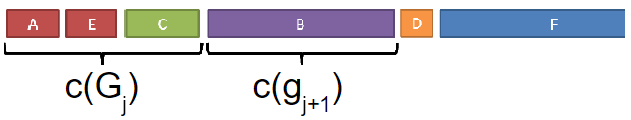
\includegraphics[width=0.8\textwidth]{\GOMPDIR/img/all-budget-good.png}
  \label{fig:all-budget-good}
}

\subfloat[Illustration of Doubling Algorithm Cost Constraint]{
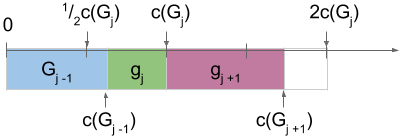
\includegraphics[width=0.8\textwidth]{\GOMPDIR/img/doubling-algo.png}
  \label{fig:doubling-algo}
}

\caption{Doubling Algorithm (b) has better anytime behaviors 
than greedy algorithm with no cost constraints (a).}
\label{fig:doubling}
\end{figure}


\begin{algorithm}[tb]
\caption{Forward Regression with Doubling Modification}
 \label{alg:greedy.doubling}
\begin{algorithmic}[1]
	\STATE {\bfseries Input:} Objective function $F$, elements $X$, minimum cost $c_{\textrm{min}}$.
	\STATE {\bfseries Output:} A sequence $G = g_1, g_2, ..., g_{J}$ of elements.
   For each $j \leq J$, a parameter  $w(G_j)$ for the elements $G_j =g_1,..., g_j$ for maximizing $F$. 
    \STATE Set $g_1 = \underset{x \in X,\ c(x) \le c_{\textrm{min}}}{\argmax} \frac{F(\{x\})}{c(x)}$.
    \STATE Set $G_1 = [g_1]$ as a one-element sequence.
    \STATE Set $w(G_1)$ be the parameter associated with $g_1$ to optimize $F$.
 \FOR {$j = 2,...,J$}
    \FOR {$g \notin G_{j-1}$, $c(g) \le c(G_{j-1})$}
        \STATE Compute $F(G_{j-1} \oplus g)$ and the associated parameter $w(G_{j-1} \oplus g)$.  
    \ENDFOR
    \STATE $g_{j} = \argmax \limits_{g = \mathcal{G}_1, ... , \mathcal{G}_J, g\notin G_{j-1}, c(g) \le c(G_{j-1})} 
	\frac{F(G_{j-1} \oplus g) - F(G_{j-1})}{c(g)}$.
   \STATE Append $g_j$ to the sequence: $G_{j} = G_{j-1} \oplus g_{j}$.
   \STATE Record $w(G_j) = w(G_{j-1} \oplus g)$.
 \ENDFOR
\end{algorithmic}
\end{algorithm}

 
\begin{definition} 
\label{def:greedy.doubling-capable}
Let $G = (g_1, \ldots)$ be the sequence selected by the doubling
algorithm.  The set $X$ and function $F$ are \textit{doubling capable}
if, at every iteration $j$, the following set is non-empty:
$
\{x \mid x \in X \setminus G_{j-1},\ c(x) \le c(G_{j-1})\}
$
\end{definition}

\begin{theorem}
\label{thm:greedy.doubling-greedy-bound-approx}
Let $G = (g_1, \ldots)$ be the sequence selected by the doubling
algorithm (Algorithm~\ref{alg:greedy.doubling}).  Fix some $B >
c_{\textrm{min}}$.  Let $F$ be $\gamma$-approximately
submodular as in Definition~\ref{def:greedy.approx-submodularity}.
For any sequence $S$,
\[
F(G_{\at{B}}) > \left(1 - e^{-\frac{\gamma^2}{1+\gamma}} \right) F(S_{\at{\frac{B}{4}}}).
\]
\end{theorem}
\begin{proof}
Doubling capable easily leads to the observation that for all budgets $B$, there exists an index $j$ such that
$\frac{B}{2} \leq c(G_j) < B$.
Choose $K$ and $k$ to be  the largest integers such that
$\frac{B}{2} \leq c(G_K) < B$ and 
$\frac{B}{8} \leq c(G_k) < \frac{B}{4}$. Since at each step we at most double the 
total cost and $4c(G_k) < B$, we observe $K \geq k+2$. 
%Let $\Delta C$ denote the cost difference $c(G_K) - c(G_k)$.
For each $j$, define $s_j = \frac{F(G_{j+1}) - F(G_{j})}{c(g_{j+1})}$ as the best 
rate of improvement among the items Doubling Algorithm is allowed to consider
after choosing $G_j$. 
Consider the item $x$ in sequence $S_{\at{\frac{B}{4}}}$ of the maximum cost. 

(Case 1) If $c(x) \leq c(G_k)$, then
every item in $S_{\at{\frac{B}{4}}}$ was a candidate for $g_{j}$ for all $j=k+1,..., K$. 
So by approximate submodularity from Equation~\ref{def:greedy.approx-submodularity}, we have 
\begin{align}
\label{eq:sub-additive}
F(S_{\at{\frac{B}{4}}}) \leq F(S_{\at{\frac{B}{4}}} \cup G_{j}) \leq F(G_j) + \frac{B s_j}{4 \gamma}.
\end{align}
Then using the standard submodular maximization proof technique, we define
\mbox{$\Delta _j = F(S_{\at{\frac{B}{4}}}) - F(G_j)$}. Applying $s_j = \frac{\Delta _{j} - \Delta_{j+1}}{c(g_{j+1})}$ in the above inequality, 
we have
\mbox{$\Delta _{k+j} \leq \Delta_k \prod _{j=k+1}^{k+j} ( 1 - \gamma \frac{ 4 c(g_{j})}{B})$}. Maximizing the 
inequality by setting $c(g_{j}) = \frac{B}{K-k} \leq \frac{c(G_K) - c(G_k)}{4 (K-k)}$, 
and using $(1- z/l)^l < e^{-z}$, we have 
\mbox{$F(G_K) > (1 - e^{-\gamma}) F(S_{\at{\frac{B}{4}}}).
$}

From now on, we assume that $c(x) > c(G_k)$ and consider 
two cases by comparing $c(g_{k+2})$ and $c(G_{k})$. 

(Case 2.1) If $c(g_{k+2}) \geq c(G_{k})$, then 
$c(G_K) - c(G_{k+1}) \geq c(g_{k+2}) \geq c(G_k)$. 
Since $c(G_{k+1}) \leq 2 c(G_k)$ and $c(x) > c(G_k)$, 
we have $c(G_K) - c(G_{k+1}) \geq \frac{B}{2} - 2c(G_k)$.
So \mbox{$c(G_K) - c(G_{k+1}) \geq \max ( c(G_k), \frac{B}{2} - 2c(G_k) ) \geq \frac{B}{6}$}. 
Thus, using the same proof techniques as in case 1, we can analyze the ratio between $\Delta_{k+1}$ and $\Delta_K$, and have:
\mbox{$
F(G_K) > (1 - e^{-\frac{2}{3} \gamma}) F(S_{\at{\frac{B}{4}}}).
$}

(Case 2.2) 
Finally, if \mbox{$c(g_{k+2}) < c(G_k) < c(x) < c(G_{k+1})$},
$g_{k+2}$ was a candidate for $g_{k+1}$, and $x$ was a candidate for 
$g_{k+2}$. 
For an item $y$, let 
\mbox{$r(y^j)= \frac{F(G_{j} \cup \{ y \}) - F(G_j)}{c(y)}$} 
be the improvement rate of item $y$ at $G_j$. 
Then we have \mbox{$r(g_{k+1}^k) > r(g_{k+2}^k)$} and \mbox{$r(g_{k+2}^{k+1}) > r(x^{k+1})$}. 
Since the objective function is increasing, we have 
\mbox{$r(x^k) c(x) \leq r(x^{k+1})c(x) + r(g_{k+1}^k)c(g_{k+1})$},
so that 
\mbox{$r(x^k) \leq r(x^{k+1}) + r(g_{k+1}^k) \frac{c(g_{k+1})}{c(x)}$}.
Then by the definition of $\gamma$ in Equation~\ref{def:greedy.approx-submodularity}, we have 
$ \gamma r(g^{k+1}_{k+2}) \leq r(g_{k+2}^k)$. Hence we have 
$ \gamma r(x^{k+1}) \leq  r(g_{k+1}^k)$, which leads to 
\mbox{$r (x^k) \leq r(g_{k+1}^k) (\frac{1}{\gamma} + \frac{c(g_{k+1})}{c(x)} ) \leq r(g_{k+1}^k) (1 + \frac{1}{\gamma})$}. Then
inequality~(\ref{eq:sub-additive}) holds with a coefficient adjustment and becomes
$
F(S_{\at{\frac{B}{4}}}) \leq F(G_k) + \frac{B s_k (1+\gamma)}{4 \gamma^2}.
$
Noting that the above inequality holds for all $j=k+1, ..., K$, we can replace the constant $\gamma$ in the 
proof of case $1$ with $\frac{\gamma^2}{1+\gamma}$ and have the following bound:\mbox{
$
F(G_K) > (1 - e^{-\frac{\gamma^2}{1+\gamma} }) F(S_{\at{\frac{B}{4}}}).
$}

\end{proof}


% terms, assumption, lemma
% Proof of the main lemma;

\section{EXPERIMENTS}
\label{sec:experiment}

\begin{table*}
\caption{Test time 0.97-Timeliness measurement of different methods on \Grain. We break
 the methods into OMP, FR and Oracle family: e.g., ``Single" in the G-CS-OMP family means G-CS-OMP-Single, and ``FR" in the Oracle family means the oracle curve derived from G-FR. }
\label{tab:grain_auc} 
\begin{center}
\resizebox{\textwidth}{!}{
\begin{tabular}{cccc|c|cc|c}
\multicolumn{4}{c|}{CS-G-OMP-Variants} &
\multicolumn{1}{c|}{CS-G-FR} &
\multicolumn{2}{c|}{Oracles} &
\multicolumn{1}{c}{Sparse} \\
	CS-G-OMP & 
	Single & 
	No-Whiten & 
	G-OMP & 
	\; & 
	FR Oracle &
	OMP Oracle &
  \; \\
  \hline
	\textbf{0.4406} & %G-OMP & 
	0.4086 &%G-OMP-Single & 
	0.4340 &%G-OMP-No-Whiten & 
	0.4073 &%G-OMP-Ignore-Cost & 
	\textbf{0.4525} &%G-FR 		& 
	\textbf{0.4551} & %FR Oracle \\
	0.4508 & % OMP oracle
  0.3997 \\
\end{tabular}
}
\end{center}
\end{table*}

\begin{table*}
\caption{Test time 0.99-Timeliness measurement of different methods on \YahooLTR.}
\label{tab:yahoo_auc} 
\begin{center}
\resizebox{\textwidth}{!}{
\begin{tabular}{c|cccc|c|cc|c}
Group &
\multicolumn{4}{c|}{CS-G-OMP-Variants} &
\multicolumn{1}{c|}{CS-G-FR} &
\multicolumn{2}{c|}{Oracles} &
\multicolumn{1}{c}{Sparse} \\
	Size &
	CS-G-OMP & 
	Single & 
	No-Whiten & 
	G-OMP & 
	\; & 
	FR &
	OMP &
  \; \\
\hline
	5      & %Group Size
	\textbf{0.3188} & %G-OMP & 
	0.3039 &%G-OMP-Single & 
	0.3111 &%G-OMP-No-Whiten & 
	0.2985 &%G-OMP-Ignore-Cost & 
	\textbf{0.3222} &%G-FR 		& 
	\textbf{0.3225} & % FR oracle
	0.3211 & %Oracle \\  
  0.2934 \\

	10      & %Group Size
	\textbf{0.3142} & %G-OMP & 
	0.3117 &%G-OMP-Single & 
	0.3079 &%G-OMP-No-Whiten & 
	0.2909 &%G-OMP-Ignore-Cost & 
	\textbf{0.3205} &%G-FR 		& 
	\textbf{0.3207} & % FR oracle
	0.3164 & %Oracle \\  
  0.2858 \\

	15      & %Group Size
	\textbf{0.3165} & %G-OMP & 
	0.3159 &%G-OMP-Single & 
	0.3116 &%G-OMP-No-Whiten & 
	0.2892 &%G-OMP-Ignore-Cost & 
	\textbf{0.3213} &%G-FR 		& 
	\textbf{0.3213} & % FR oracle
	0.3177 & %Oracle \\  
  0.2952 \\

	20     & %Group Size
	\textbf{0.3161} & %G-OMP & 
	0.3124 &%G-OMP-Single & 
	0.3065 &%G-OMP-No-Whiten & 
	0.2875 &%G-OMP-Ignore-Cost & 
	\textbf{0.3180} &%G-FR 		& 
	\textbf{0.3180} & % FR oracle
	0.3163 & %Oracle \\ 
  0.2895 \\

\end{tabular}
}
\end{center}
\end{table*}


\begin{figure}[ht!]
\centering
\subfloat[Training Time OMP vs. FR (\Grain)]{
  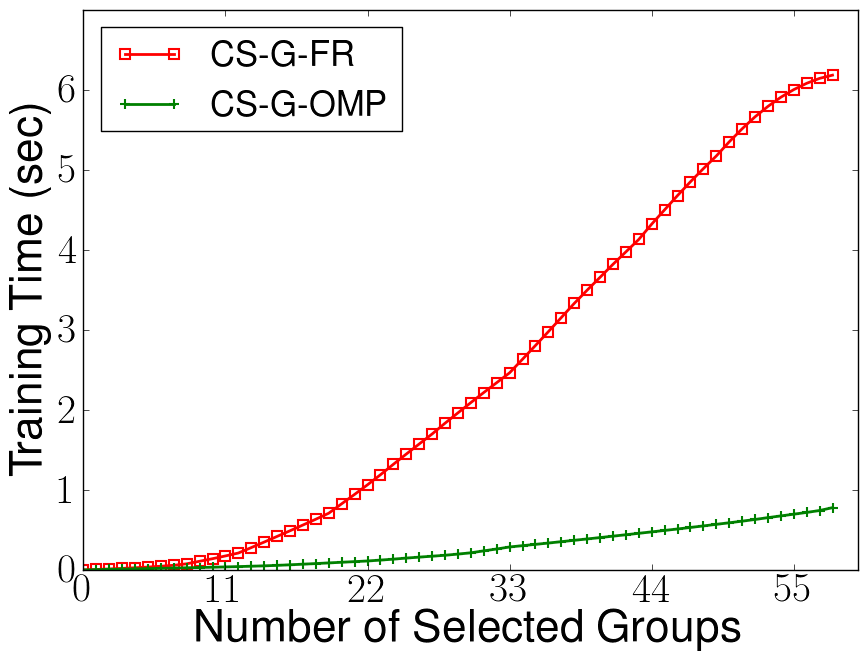
\includegraphics[width=0.44\textwidth,keepaspectratio]{\GOMPDIR/img/set1_exp4.png}
}
~
\subfloat[Training Time OMP vs. FR (\YahooLTR)]{
  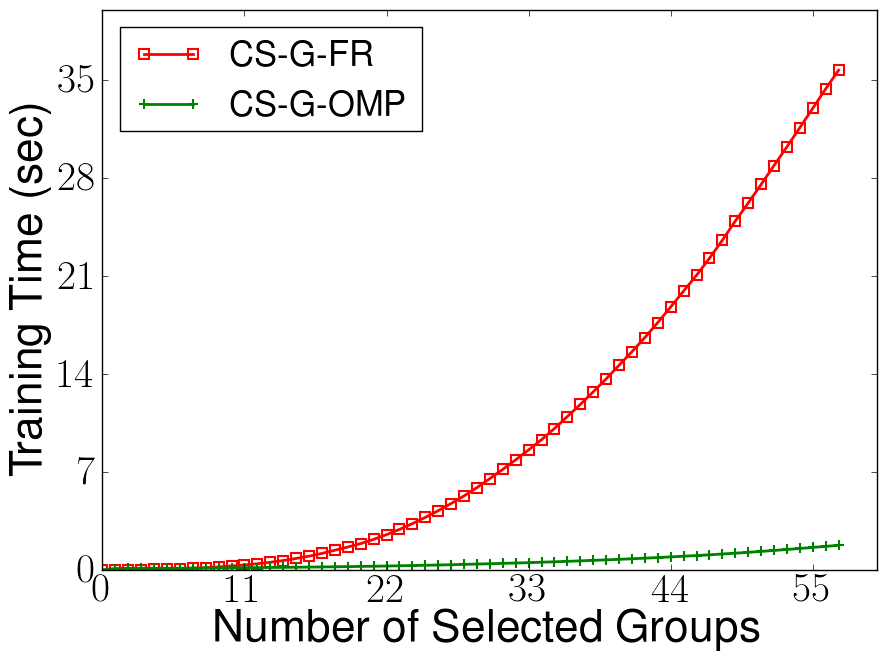
\includegraphics[width=0.44\textwidth,keepaspectratio]{\GOMPDIR/img/set1_size10_exp4.png}
}
\caption{The training time vs. the number of feature groups selected with two algorithms: CS-G-FR and 
CS-G-OMP. CS-G-OMP achieves a 8x and 20x overall training time speed-up 
on \Grain\, and \YahooLTR.} 
\label{fig:run_time}
\end{figure}

\subsection{DATA-SETS AND SET-UP}
We experiment our methods for anytime linear prediction on two real-world data-sets,
each of which has a significant number of feature groups with associated costs. 

\begin{itemize}[leftmargin=*]
\item \textbf{Yahoo! Learning to Rank Challenge} \citep{yahoo_ltr}
contains 883k web documents, each of which has a relevance score in $\{0, 1, 2, 3, 4\}$. Each of the 501 document features has an associated computational cost in 
$\{ 1, 5, 20, 50, 100, 150, 200\}$; the total feature cost is around 17K. The original data-set has no feature group structures, so we generated random group structures by grouping features of the same cost into groups of a given size $s$.\footnote{We experiment on group sizes $s \in \{ 5, 10, 15, 20 \}$. We choose regularizer 
$\lambda = 10^{-5}$ based on validation. We use 
$s=10$ for qualitative results such as plots and illustrations, but we report quantitative results for all group size $s$. For our quantitative results, we report the average test performance. The initial risk is $R(\emptyset)=0.85$.}

\item \textbf{Agriculture} is a proprietary data-set that contains 510k data samples, 328 features, and 57 feature groups. Each sample has a binary label in $\{1, 2\}$. Each feature group has an associated cost measured in its 
average computation time.\footnote{
There are 6 groups of size 32; the other groups have sizes between 1 and 6. 
The cost of each group is its expected computation time in seconds, ranging between 0.0005 and 0.0088; the total feature cost is 0.111. 
We choose regularizer $\lambda = 10^{-7}$. The data-set is 
split into five 100k sets, and the remaining 10k are used for validation. We report the cross validation results on the five 100K sets as the test results. The initial risk is $R(\emptyset) = 0.091$.}
\end{itemize}

\subsection{EVALUATION METRIC, BASELINE AND ORACLE}
\label{sec:timeliness}
\begin{figure}[ht!]
\centering
\subfloat[Plateau Effect and $\alpha$-Stopping Costs]{
 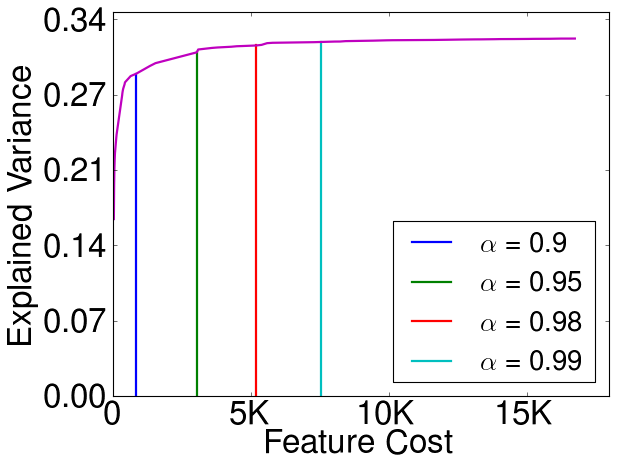
\includegraphics[width=0.44\textwidth,keepaspectratio]{\GOMPDIR/img/timeliness.png}
 \label{fig:timeliness_a}
}
~
\subfloat[Importance of Costs (CS-G-OMP vs. G-OMP)]{
 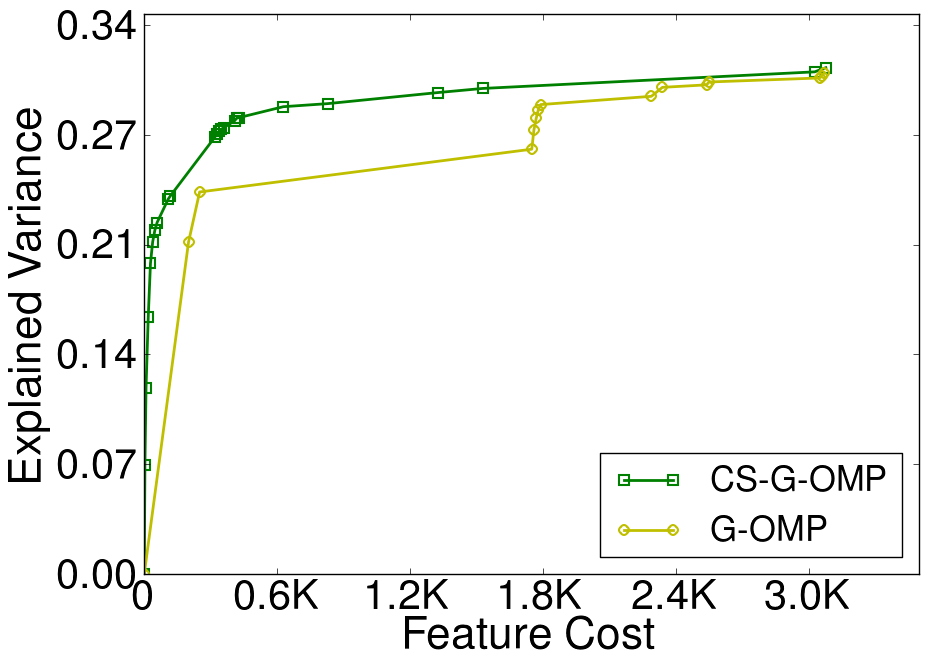
\includegraphics[width=0.44\textwidth,keepaspectratio]{\GOMPDIR/img/set1_size10_exp2.png}
 \label{fig:cost_vs_no_cost}
}
\label{fig:timeliness}
\caption{(a) Explained Variance vs. Cost curve of CS-G-OMP in
\YahooLTR. Vertical lines mark different $\alpha$-stopping costs.  (b) Explained Variance vs. Cost curve of CS-G-OMP and G-OMP on \YahooLTR\, set 1 with individual group size $s=10$, stopped at 0.97-stop cost.}
\end{figure}

Following the practice of \cite{timeliness}, we use the area under the 
maximization objective $F$ (explained variance) vs. cost curve normalized by the total area as the 
\textit{timeliness} measurement of the anytime performance of an algorithm\footnotetext{\cite{timeliness} define \textit{timeliness} as the area under the average precision vs. time curve}. In our data-sets, the performance of linear predictors plateaus much before
all features are used, e.g., Figure~\ref{fig:timeliness_a} demonstrates this effect in \YahooLTR, where the last one percent of total improvement is bought by half of the total feature cost. Hence the majority of the timeliness measurement is from the plateau performance of linear predictors. The difference between timeliness of different anytime algorithms diminishes due to the plateau effect. Furthermore, the difference vanishes as we include additional redundant high cost features. To account for this effect, we 
stop the curve when it reaches the plateau.
We define an \textit{$\alpha$-stopping cost} for parameter $\alpha$ in $[0,1]$ as the cost at which our CS-G-OMP achieves $\alpha$ of the final objective value in training and ignore the objective vs. cost curve after
the $\alpha$-stopping cost. We call the timeliness measure on the shortened curve 
as \textit{$\alpha$-timeliness}; 1-timeliness equals the normalized area under the full curve and 0-timeliness is zero. If a curve does not pick a group at $\alpha$-stopping cost, we linearly interpolate the objective value at the stopping cost to 
computr timeliness. 
We say an objective vs. cost curve has reached its final plateau if at least 95\% of the total 
objective has been achieved and the next 1\% requires more than 20\%
feature costs. (If the plateau does not exist, we use $\alpha = 1$.) Following this rule, we choose $\alpha = 0.97$ for \Grain\ and $\alpha = 0.99$ for \YahooLTR.

Since an exhaustive search for the best feature sequencing is intractable, 
we approximate with the \textbf{Oracle} anytime performance following the approach of \cite{timeliness}. Given an objective vs. cost curve of a sequencing, we reorder the feature groups in descending order of their marginal benefit per unit cost, assuming that the marginal benefits stay the same after reordering. We specify which sequencing is used for creating \textbf{Oracle} in Section~\ref{sec:selection_methods}. 
For baseline performance, we use cost-weighted Group Lasso \citep{group_lasso}, which
scales the regularization constant of each group with the cost of the group. We note that the cascade design by 
\cite{chen:12} can be reduced to this baseline if we enforce
linear prediction. 
More specifically, the baseline solves the following minimization problem:
\mbox{$
  \min _{w \in \mathbb{R}^{D}} \Vert Y -
    Xw \Vert^2_2 + \lambda
    \sum _{j=1}^J c(\mathcal{G}_j) \Vert w _{\mathcal{G}_j} \Vert _2,
$}
and we vary value of regularization constant
$\lambda$ to obtain lasso paths. We call this baseline algorithm \textbf{Sparse}\footnote{We use an off-the-shelf software, 
SPAMS (SPArse Modeling Software \citep{spams}), to solve the optimization.}.


\subsection{FEATURE COST}
Our proposed CS-G-OMP differs from Group Orthogonal Matching Pursuit (G-OMP) \citep{gomp} in that G-OMP does not consider feature costs when evaluating features. We show that this difference is crucial for anytime linear prediction. In Figure~\ref{fig:cost_vs_no_cost}, we compare the objective vs. costs curves of CS-G-OMP and G-OMP that are stopped at 0.97-stopping cost on \YahooLTR. As expected, CS-G-OMP achieves a
better overall prediction at every budget, qualitatively demonstrating the importance of incorporating feature costs. Table~\ref{tab:grain_auc} and Table~\ref{tab:yahoo_auc} 
quantify this effect, showing that CS-G-OMP 
achieves a better timeliness
measure than regular G-OMP. 

\subsection{GROUP WHITENING}
%Compare different normalization methods: whiten the whole data, 
%zero mean normalize, whiten each group. \and 
We provide experimental evidence that  
Group whitening, i.e., $X_g^TX_g = I_{D_g}$ for each group $g$, is a key assumption of both this work and previous feature group selection literature  by \cite{gomp, log_gomp}.
In Figure~\ref{fig:whiten_vs_no_whiten}, we compare 
anytime prediction performances using group whitened data 
against those using the common  
normalization scheme where each feature dimension
is individually normalized to have zero mean and unit variance. 
The objective vs. cost curve qualitatively shows that group whitening consistently results in the better predictions.
This behavior is expected from data-sets whose feature groups contain correlated features, e.g., group whitening effectively prevents selection step $(*)$ from overestimating the predictive power of feature groups of repeated good features. Table~\ref{tab:grain_auc} and Table~\ref{tab:yahoo_auc} demonstrate quantitatively the consistent better timeliness performance of CS-G-OMP over that of CS-G-OMP-no-whiten. 


\begin{figure}[ht!]
\centering
\subfloat[Group Whiten vs. No-Whiten (\Grain)]{
  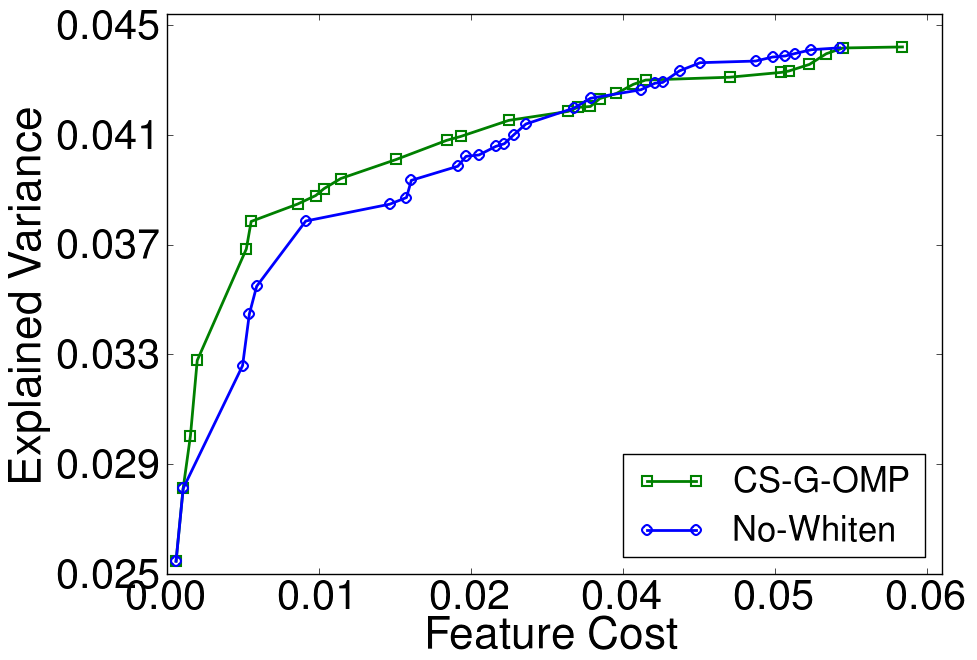
\includegraphics[width=0.44\textwidth,keepaspectratio]{\GOMPDIR/img/set1_exp1.png}
}
~
\subfloat[Group Whiten vs. No-Whiten (\YahooLTR)]{
  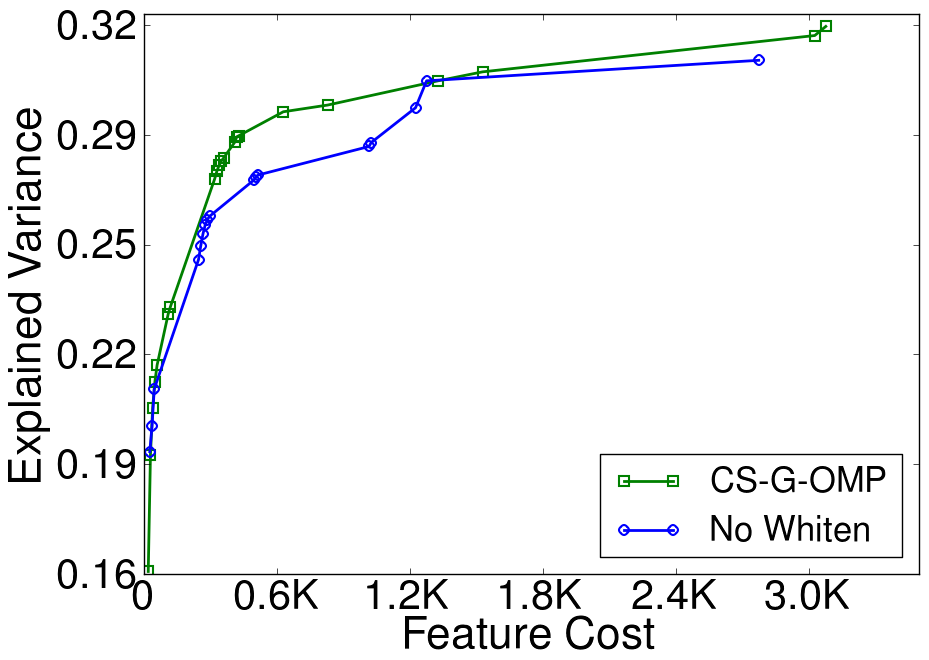
\includegraphics[width=0.44\textwidth,keepaspectratio]{\GOMPDIR/img/set1_size10_exp1.png}
}
\caption{Explained Variance vs. Feature Cost curves on \Grain\, (a) and \YahooLTR\, (b)  comparing group whitening with no group whitening. The curves stop at 0.97-stopping cost.}
\label{fig:whiten_vs_no_whiten}
\end{figure}


\subsection{SELECTION CRITERION VARIANTS}
\label{sec:selection_methods}
%FR vs OMP; group vs single

This section compares CS-G-OMP and CS-G-FR, along with 
variants of these two methods and the baseline, Sparse. 
We formulated the variant of CS-G-OMP, \textit{single}, in Section~\ref{sec:gomp_method} and it intuitively chooses feature groups of the best single feature dimension per group cost. Our experiments show that this modification degrades prediction performance of CS-G-OMP. 
%If we enforce linear prediction, cascade design by \cite{cai:15} can be reduced to a greedy method whose criteria is the G-OMP criteria subtracted by a function of the feature cost. However, this method requires careful tuning of the 
Since FR directly optimizes the objective at each step, we expect CS-G-FR to perform the best and use its curve to compute the \textbf{Oracle} curve as an approximate to the best achievable performance.

In Figure~\ref{fig:selection_methods}, we evaluate CS-G-FR, CS-G-OMP and CS-G-OMP-single based on the objective in Theorem~\ref{thm:main}, i.e., explained variance vs. feature cost curves. 
CS-G-FR, as expected, outperforms all other methods. CS-G-OMP outperforms the baseline method, Sparse, and the CS-G-OMP-Single variant. 
The performance advantage of CS-G-OMP over CS-G-OMP-Single is much clearer in the \Grain\ data-set than in the \YahooLTR\ data-set. \Grain\ has a natural group structure which may contain correlated features in each group. \YahooLTR\ has a randomly generated group structure whose features were filtered by feature selection before the data-set was published \citep{yahoo_ltr}. CS-G-FR and CS-G-OMP outperform the baseline algorithm, Sparse. We speculate that linearly scaling group regularization constants by group costs did not enforce Group-Lasso to choose the most cost-efficient features early. 
The test-time timeliness measures of each of the methods are recorded in Table~\ref{tab:grain_auc} and Table~\ref{tab:yahoo_auc},
and quantitatively confirm the analysis above. Since \Grain\, and \YahooLTR\, are originally a classification and a ranking data-set, respectively, we also report in Figure~\ref{fig:selection_methods} the performance using classification accuracy and NDCG@5. This demonstrates the same qualitatively results as using explained variants. 

%We note that on the two real-world data-sets, Doubling Algorithm acts identically to CS-G-FR after few initial selections, an expected result because real-world feature effectiveness does not grow exponentially in cost, so that the most cost-efficient features become available to Doubling after few steps. 


\begin{figure}[ht!]
\centering
\subfloat[FR vs. OMP vs. Sparse (\Grain)]{
  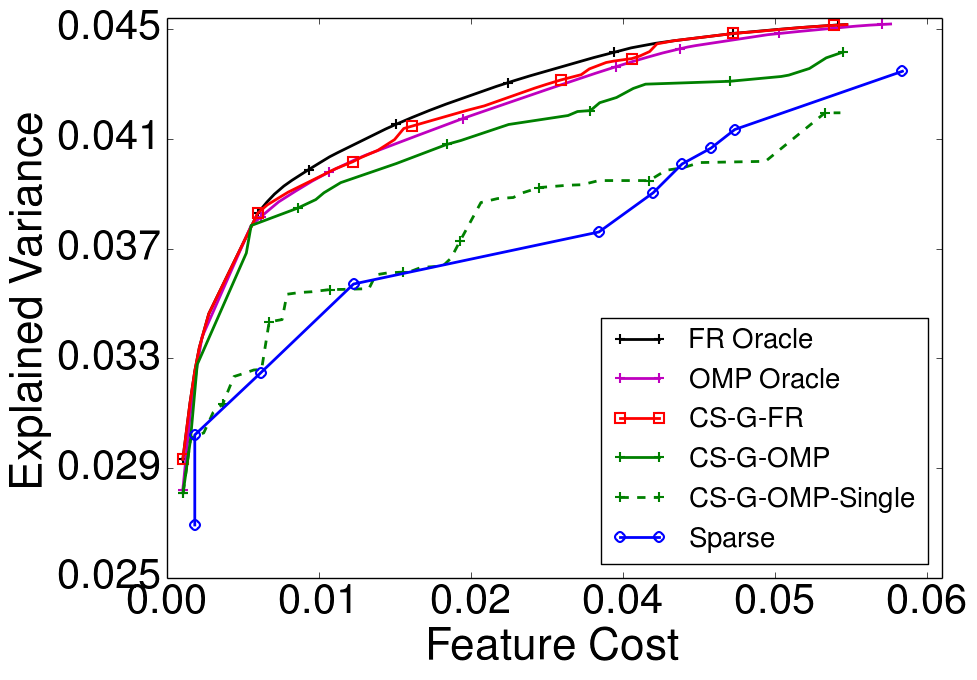
\includegraphics[width=0.44\textwidth,keepaspectratio]{\GOMPDIR/img/set1_exp3.png}
}
~
\subfloat[FR vs. OMP vs. Sparse (\YahooLTR)]{
  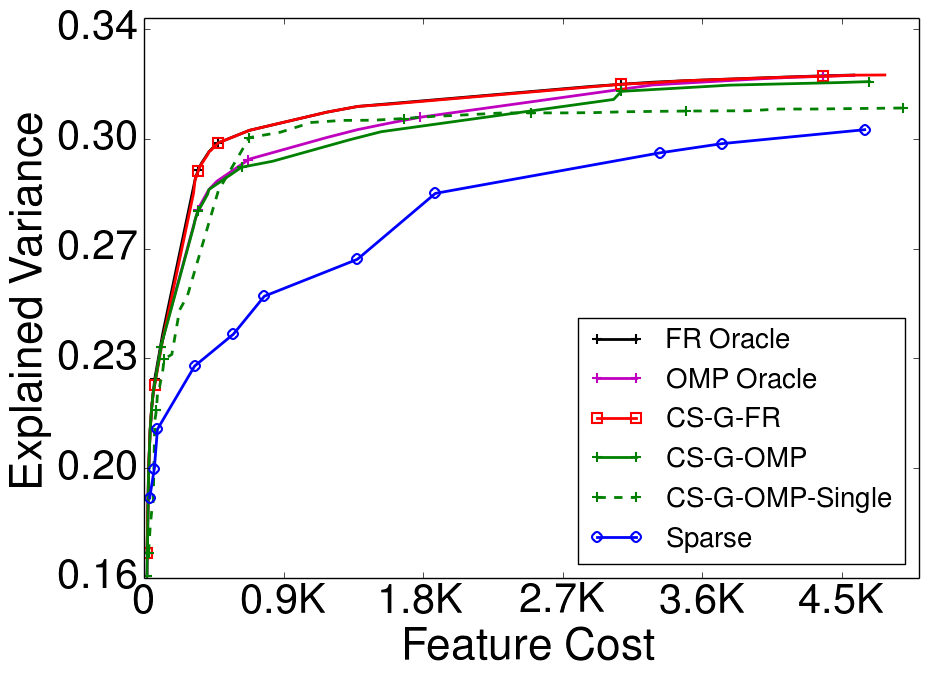
\includegraphics[width=0.44\textwidth,keepaspectratio]{\GOMPDIR/img/set1_size10_exp3.png}
}

\subfloat[FR vs. OMP vs. Sparse (\Grain)]{
  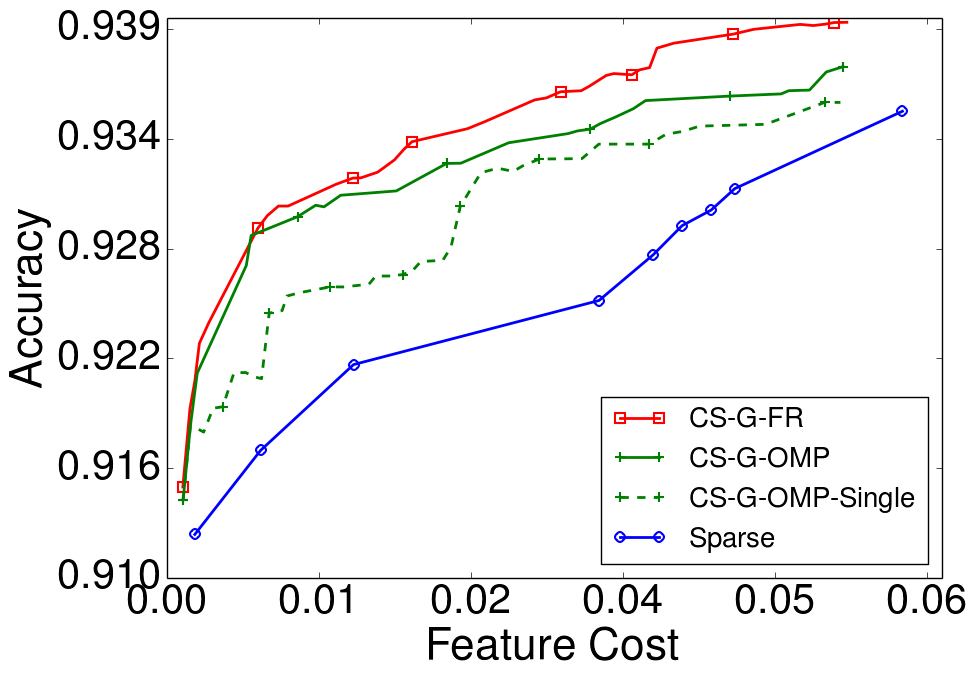
\includegraphics[width=0.44\textwidth,keepaspectratio]{\GOMPDIR/img/set1_exp5.png}
}
~
\subfloat[FR vs. OMP vs. Sparse (\YahooLTR)]{
  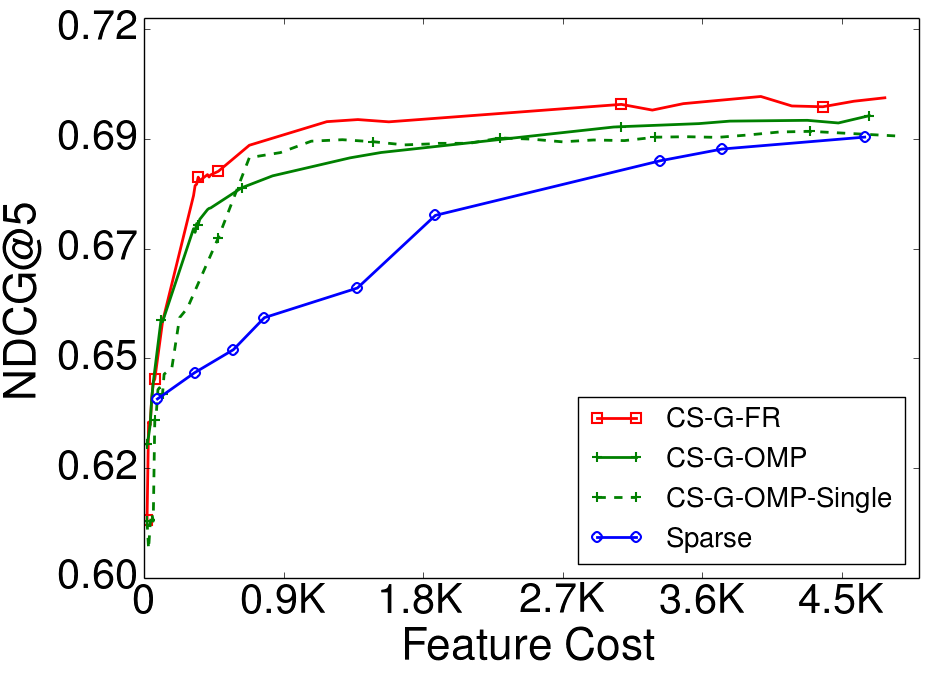
\includegraphics[width=0.44\textwidth,keepaspectratio]{\GOMPDIR/img/set1_size10_exp5.png}
}

\caption{(a),(b): Explained Variance vs. Feature Cost curves on 
\Grain\, and \YahooLTR (group-size=10), 
using CS-G-OMP, CS-G-FR and their Single variants. Curves stop at 0.97 and 0.98 stopping costs. (c),(d): Same curve with the natural objectives of the data-sets: accuracy and NDCG@5.} 
\label{fig:selection_methods}
\end{figure}

As expected, when compared against CS-G-OMP, CS-G-FR consistently chooses more cost-efficient features at the cost of a longer training time.
In the context of linear regression, let us assume that the group sizes are 
bounded by a constant when we are to select the number 
$K$ feature group. We can then compute a new model of $K$  groups in $O(K^2N)$ using
Woodbury's matrix inversion lemma, evaluate it in $O(KN)$, and compute the gradients with respect to the weights of unselected groups in $O(N(J-K))$. Thus, CS-G-OMP requires $O(K^2N + JN)$ at step $K=1,2,3,..., J$ and CS-G-FR requires $O((J-K)K^2N)$, so the total training  complexities for CS-G-OMP and CS-G-FR are $O(J^3N)$ and $O(J^4N)$, using $\sum_{K=1}^J K^2 = \frac{1}{6}J(J+1)(2J+1)$ and $\sum _{K=1}^J K^3 = \frac{1}{4}J^2(J+1)^2$. 
We also show this training complexity gap empirically in Figure~\ref{fig:run_time}, which plots the curves of training time vs. number of feature groups selected. When all feature groups are selected, CS-G-OMP achieves a 8x speed-up in \Grain\ over CS-G-FR. In \YahooLTR, CS-G-OMP achieves a speed-up factor between 10 and 20; the smaller the sizes of the groups, the larger speed-up due to the increase in the number of groups. Both greedy methods are much faster than the Lasso path computation using SPAMS, however. 






\section{Additional Proof Details}
\label{sec:gomp_proof_II}
This section describes a functional boosting view of selecting features for generalized linear models of one-dimensional response. We then prove Lemma~\ref{lemma:smoothness} and Lemma~\ref{lemma:convexity} for this more general setting. These more general
results in turn extend Theorem~\ref{thm:main} to generalized 
linear models.

\subsection{Functional Boosting View of Feature Selection}
\label{sec:functional}

We view each feature $f$ as a function 
$h_f$ that maps sample $x$ to $x_f$. We define $f_S: \R^{D} \rightarrow \R$ 
to be the best linear predictor using features in $S$, i.e., $f_S(x) \triangleq w(S)^Tx_S$. For each feature dimension $d \in D$, the coefficient of 
$d$ is in $w(S)$ is $w(S)_d = f_S(e_d)$, where $e_d$ is the $d^{th}$ dimensional unit vector. So $\Vert w(S) \Vert_2^2 = \sum _{d = 1}^D \Vert f_S(e_d) \Vert _2^2$. 
Given a generalized linear model with link function $\nabla \Phi$, 
the predictor is $E[ y | x ] = \nabla \Phi(w^Tx)$ for some $w$ and the calibrated loss is $r(w) = \sum _{i=1}^n (\Phi(w^Tx_i) - y_iw^Tx_i)$. 
Replacing $f_S(x_i) = w(S)^Tx_i$, we have 
\begin{align}
	r(w(S)) = \sum _{i=1}^n (\Phi(f_S(x_i)) - y_if_S(x_i)).
	\label{eq:glm_loss_general}
\end{align}
Note that the risk function in Equation~\ref{eq:risk} can be rewritten as 
the following to resemble Equation~\ref{eq:glm_loss_general}:
\begin{align}
 R(S) = 
 	\mathcal{R}[f_S] =& \frac{1}{n} \sum _{i=1}^n (\Phi(f_S(x_i)) - y_i^Tf_S(x_i)) \notag \\
    &{} + \frac{\lambda}{2} \sum _{d = 1}^D \Vert f_S(e_d) \Vert _2^2 + A,
  \label{eq:min_func}
\end{align}
where $\phi(x) = \frac{1}{2}x^2$ for linear predictions and constant 
$A = \frac{1}{2n} \sum _{i=1}^n y_i^2$. 
Next we define the inner product between two functions $f, h : \R^D \rightarrow \R$ 
over the training set to be:
\begin{align}
\angleb{f, h} \triangleq \frac{1}{n} 
  \sum _{i=1}^n f(x_i)h(x_i) + \frac{\lambda}{2} \sum _{d=1}^D f(e_d)h(e_d).
\end{align}
With this definition of inner product, we can compute the derivative of 
$\mathcal{R}$:
\begin{align}
  \nabla \mathcal{R}[f]  = \sum_{i=1}^n (\nabla\Phi(f(x_i)) 
  	- y_{i})\delta_{x_i} 
    + \sum _{d=1}^D f(e_d)\delta_{e_d},
\end{align}
where $\nabla \phi(x) = x$ for linear predictions, and 
$\delta_x$ is an indicator function for $x$. 
Then the gradient of objective $F(S)$ w.r.t coefficient $w_f$ of a feature dimension  $d$ can be written as:
\begin{align}
 b_{d}^S &= - \frac{1}{n}\sum_{i=1}^n (\nabla\Phi_p(w(S)^Tx^i) - y^{i})x^i_d - \lambda w(S)_d \\
    &= - \angleb{  \nabla \mathcal{R}[f_S], h_d }.
\end{align}
In addition, the regularized covariance matrix of features $C$ satisfies,
\begin{equation}
    C_{ij} = \frac{1}{n} X_i^TX_j + \lambda I(i=j) = \angleb{ h_i, h_j},
\end{equation}
for all $i, j = 1,2,..., D$.
So in this functional boosting view,  Algorithm~\ref{algo:gomp_lm} greedily chooses group $g$ that maximizes, with a slight abuse of notation of $\angleb{ \;, \; }$,
$\Vert \angleb{ h_g , \nabla \mathcal{R}[f_S] } \Vert _2^2 / c(g)$, i.e., 
the ratio between similarity of a feature group and the functional gradient, 
measured in sum of square of inner products, and the cost of the group


\subsection{Proof of Lemma~\ref{lemma:smoothness} and Lemma~\ref{lemma:convexity}}

The more general version of Lemma~\ref{lemma:smoothness} and Lemma~\ref{lemma:convexity} assumes that the objective functional $\mathcal{R}$ 
is $m$-strongly smooth and $M$-strongly convex using our proposed inner product rule.  
$M$-strong convexity is a reasonable assumption, 
because the regularization term $\Vert w \Vert _2^2 = \sum _{d = 1}^D \Vert f_S(e_d) \Vert _2^2$ ensures that all loss functional $\mathcal{R}$ with a convex $\Phi$ 
 strongly convex. 
In the linear prediction case, both $m$ and $M$ equals $1$. 

The following two lemmas are the more general versions of Lemma~\ref{lemma:smoothness} and Lemma~\ref{lemma:convexity}.
\begin{lemma}
  Let $\mathcal{R}$ be an m-strongly smooth functional with respect to our definition of inner products. Let $S$ and $G$ be some fixed sequences. Then
  \begin{align}
   F(S) - F(G) \notag \leq \frac{1}{2m} \angleb{b^G_{G \oplus S}, C_{G \oplus S}^{-1} b^G_{G\oplus S}}
  \end{align}
  \label{lemma:smoothness_glm}
\end{lemma}
\begin{proof}
First we optimize over the weights in $S$. 
  \begin{align*}
    &{} F(S) - F(G) \\
    &= \mathcal{R}[f_G] - \mathcal{R}[f_S] 
     = \mathcal{R}[f_G] - \mathcal{R}[\sum _{s \in S} \alpha_s^T h_s] \\
    &\leq \mathcal{R}[f_G] - \min _{w : w_i^T \in \R^{d_{s_i}}, s_i \in S} 
        \mathcal{R}[ \sum _{s_i \in S} w_{s_i}^T h_{s_i}] \\
\intertext{Adding dimensions in $G$ will not increase the risk, we have: }
    &\leq \mathcal{R}[f_G] - \min _{w : w_i \in \R^{d_{s_i}}, s_i \in G \oplus S}
        \mathcal{R}[ \sum _{s_i \in G \oplus S} w_{s_i} h_{s_i}] \\
\intertext{Since $f_G = \sum _{g_i \in G} \alpha_i h_{g_i}$, we have:}
    &\leq \mathcal{R}[f_G] - \min _{w} 
      \mathcal{R}[f_G + \sum _{s_i \in G \oplus S} w_i^T h_{s_i}] \\
\intertext{Expanding using strong smoothness around $f_G$, we have:}
    &\leq \mathcal{R}[f_G] - \min _{w} (
      \mathcal{R}[f_G] + \angleb{ \nabla \mathcal{R}[f_G], 
        \sum _{s_i \in G\oplus S} w_i^T h_{s_i} } \notag \\
    &\quad + \frac{m}{2} \Vert \sum _{s_i \in G \oplus S} w_i^T h_{s_i} \Vert _2^2) \\
    &= \max_{w} - 
      \angleb{ \nabla \mathcal{R}[f_G], 
      \sum _{s_i \in G\oplus S} w_i^T h_{s_i} } 
        - \frac{m}{2} \Vert \sum _{s_i \in G \oplus S} w_i^T h_{s_i} \Vert _2^2 \\
    &= \max_w \angleb{ b^{G}_{G\oplus S}, w} - \frac{m}{2} \angleb{w, C_{G\oplus S}w}
 \end{align*}
Solving $w$ directly we have:
\begin{align*}
  F(S) - F(G) \leq \frac{1}{2m} \angleb{ b^{G}_{G\oplus S} , C_{G\oplus S}^{-1} b^{G}_{G\oplus S}}
\end{align*}
\end{proof}


%%%%%%%%%%%%% 
%%%%%  Lemma Strong convexity
\begin{lemma}
  Let $\mathcal{R}$ be a M-strongly convex functional with respect to our definition of 
  inner products. Then
    \begin{align}
      F(G_j) - F(G_{j-1}) \geq \frac{1}{2M (1 + \lambda) } \angleb{{b^{G_{j-1}}_{g_j}}, b^{G_{j-1}}_{g_j} }
    \end{align}
  \label{lemma:convexity_glm}
\end{lemma}
\begin{proof}
After the greedy algorithm chooses some group $g_j$ at step $j$, 
  we form $f_{G_j} = \sum _{\alpha _i} \alpha_i^T h_{g_i}$, such that
   \[
    \mathcal{R}[f_G] = \min _{ \alpha _i \in \R^{d_{g_i}}} 
      \mathcal{R}[ \sum _{g_i \in G_j} \alpha_i^T h_{g_i}] \leq
      \min _{\beta \in \R^{d_{g_j}}} 
    \mathcal{R}[f_{G_{j-1}} + \beta h_{g_j}]
   \]
 Setting $\beta = \arg \min _{\beta \in \R^{d_{g_j}}} 
    \mathcal{R}[f_{G_{j-1}} + \beta h_{g_j}]$, using the strongly convex condition at
      $f_{G_{j-1}}$, we have:
 \begin{align*}
    &{} F(G_j) - F(G_{j-1}) \\
    &=  \mathcal{R}[f_{G_{j-1}}] - \mathcal{R}[f_{G_j}] 
    \geq \mathcal{R}[f_{G_{j-1}}] - \mathcal{R}[f_{G_{j-1}} + \beta h_{g_j}] \\ 
    &\geq  \mathcal{R}[f_{G_{j-1}}] - 
      (\mathcal{R}[f_{G_{j-1}}] + 
        \angleb{ \nabla \mathcal{R}[f_{G_{j-1}}] , 
        \beta h_{g_j} } \notag \\
    &\quad + \frac{M}{2} \Vert \beta h_{g_j} \Vert _2^2) \\
    &=  -  \angleb{ \nabla \mathcal{R}[f_{G_{j-1}}] , 
        \beta h_{g_j} }
       - \frac{M}{2} \Vert \beta h_{g_j} \Vert _2^2 \\
    &=  \angleb{{b^{{G_{j-1}}}_{g_j}},  \beta} - \frac{M}{2} \angleb{\beta, C_{g_j} \beta} \\
    &\geq  \frac{1}{2M} \angleb{ b^{{G_{j-1}}}_{g_j}, C_{g_j}^{-1} b^{{G_{j-1}}}_{g_j}} \\
    &=  \frac{1}{2M (1+\lambda)} \angleb{{b^{{G_{j-1}}}_{g_j}}, b^{{G_{j-1}}}_{g_j}}
 \end{align*}
 The last equality holds because each group is whitened, 
 so that $C_{g_j} = (1 + \lambda) I$.
\end{proof}
Note that the $(1+\lambda)$ constant is a result of group whitening, without which
the constant can be as large as $(D_{g_j} + \lambda)$ for  the worst case where
all the $D_{g_j}$ number of features are the same. \\

The proofs above for Lemma~\ref{lemma:smoothness_glm} and~\ref{lemma:convexity_glm} are 
for one-dimensional output responses. They can be easily generalized to multi-dimensional 
responses by replacing 2-norms with Frobenius norms and vector inner-products with ``Frobenius products", i.e., the sum of the products of all elements. \\

\subsection{Proof of Main Theorem}
\label{sec:app-main-proof}
Given Lemma~\ref{lemma:smoothness_glm} and Lemma~\ref{lemma:convexity_glm}, 
the proof of Lemma~\ref{lemma:main} holds with the same analysis with a more 
general constant $\gamma = \frac{m \lambda_{min}(C)}{M(1+\lambda)}$. The following prove our main theorem~\ref{thm:main}. 
 
\begin{proof} (of Theorem~\ref{thm:main}, given Lemma~\ref{lemma:main})
\label{proof:main}
  Define $\Delta _j = F(S_{\angleb{K}}) - F(G_{j-1})$. Then we have 
  $\Delta _j - \Delta_{j+1} = F(G_{j}) - F(G_{j-1})$. By Lemma ~\ref{lemma:main}, we have:
  \begin{align*}
    \Delta_j &= F(S_{\angleb{K}}) - F(G_{j-1})\\
    &\leq \frac{K}{\gamma}
      \lbrack \frac{F(G_{j}) - F(G_{j-1})}{c(g_{j})} \rbrack 
        = \frac{K}{\gamma} \lbrack \frac{\Delta_j - \Delta_{j+1}}{c(g_j)} \rbrack
  \end{align*}
  Rearranging we get 
    $\Delta_{j+1} \leq \Delta_j ( 1 - \frac{\gamma c(g_j)}{K} )$. Unroll we get:
  \begin{align*}
    \Delta _{L+1} 
    &\leq 
      \Delta _1 \prod _{j=1}^L (1 - \frac{\gamma c(g_j)}{K})
    \leq \Delta _1 ( \frac{1}{L} \sum _{j=1}^L (1- \frac{\gamma c(g_j)}{K})) ^L\\
    &= \Delta _1 (1 - \frac{B\gamma}{L K})^L < \Delta_1 e^{- \gamma \frac{B}{K}}
  \end{align*}
  By definition of $\Delta_1$ and $\Delta_{L+1}$, we have:
  \begin{align*}
    F(S_{\angleb{K}}) - F(G_{\angleb{B}}) < F(S_{\angleb{K}}) e^{- \gamma \frac{B}{K}}
  \end{align*}
  The theorem follows and linear prediction is the special case that $m = M$.
\end{proof}

%\section{Appendix B: Generalized Linear Model with Multi-Dimensional Response}
\section{Extension to Generalized Linear Model}
\label{sec:extension}
While we only formulated the feature group sequencing problem in linear prediction setting previously, we can extend our algorithm for generalized linear models\cite{glm} and multi-dimensional responses. In general, we assume that we have $P$ dimensional responses, and predictions are of the form $E[y | x ] = \nabla \phi( W x)$, for some known convex function $\phi : \mathbb{R}^P \rightarrow \mathbb{R}$, and an unknown coefficient $P\times D$ matrix, $W$. Thus, the generalized linear
prediction problem is to minimize over coefficient matrix $W: P\times D$:
\begin{align}
	\textbf{r}(W) = \frac{1}{n} \sum _{i=1}^n (\phi(Wx^i) - {y^i}^TWx^i) 
		+ \frac{\lambda}{2} \Vert W\Vert^2_F,
		\label{eq:glm_loss}
\end{align}
where $\lambda$ is the regularization constant for Frobenius norm of the coefficient 
matrix. In particular, we have $\phi(x) = \frac{1}{2}x^2$ for linear prediction. 
The risk of a collection of features, $S$, is then 
\mbox{$R(S) = \underset{W : \forall g \notin S  W_g = \textbf{0} }{\min} \textbf{r}(W)$}. 
To extend CS-G-OMP to feature sequencing in this general setting, we again, at each step,
take gradient of the objective $\textbf{r}$ w.r.t. $W$, and choose the feature group that has the largest ratio of group gradient Frobenius norm square to group cost. More specifically, after choosing groups in $G$, we have a best coefficient matrix restricted to G, $W(G)$. Then we compute the gradient w.r.t. $W$ at $W(G)$ (we keep the convention that unselected groups have zero coefficients) as:
\begin{align}
	\nabla \textbf{r}(W) = \frac{1}{n} \sum _{i=1}^n (\nabla \phi(Wx^i) - y^i){x^i}^T + \lambda W;
	\label{eq:glm_gradient}
\end{align}
we then evaluate $\Vert \textbf{r}(W)_g \Vert_F^2 / c(g)$ for each feature group $g$, and add the maximizer to the selected groups to create new models. 
Algorithm~\ref{algo:gomp_glm} demonstrates the procedure. 

Our theoretical result Theorem~\ref{thm:main} can also be proven in this general setting. 
Proofs of Lemma \ref{lemma:smoothness} and \ref{lemma:convexity}) in appendix are readily for generalized linear models\footnote{Inner products, $\angleb{\bullet, \bullet}$, in Lemma \ref{lemma:smoothness} and \ref{lemma:convexity} now represent Frobenius products, which are sums of element-wise products of matrices.}. Given these two lemmas, our proofs of Lemma~\ref{lemma:main}
and Theorem~\ref{thm:main} hold as they are. 


%%%%%%%%%%%%%%%%%%%%%%%%%
%% Algorithm statement %%
%%%%%%%%%%%%%%%%%%%%%%%%%
%\IncMargin{1em}
%\begin{algorithm}[h]
%  \SetKwInOut{Input}{input}\SetKwInOut{Output}{output}
%
%  \Input{The data matrix $\XX = [ \textbf{f}_1, ..., \textbf{f}_D ] \in \R^{n \times D}$,
%    with group structures, such that for each group $g$,
%    $\XX^T_{g}\XX_{g} = I _{D_g}$.     
%    The cost $c(g)$ of each group $g$. 
%    The response matrix $\YY \in \{0, 1\}^{n \times P}$.
%    The link function $\nabla \Phi$.
%    Regularization constant $\lambda$.
%  }
%  \Output{
%    A sequence $((G_j, W_j))_j$, where 
%      $G_j = (g_1, g_2, ..., g_j)$ 
%    is the sequence of first $j$ selected feature groups, $g_1, g_2, ..., g_j$, and 
%      $W_j: P\times D$ restricted to features in $G_j$ 
%      is the associated coefficient matrix.
%  }
%
%  $G_0 = \emptyset$; $W_0 = \textbf{0}$\;
%  \For{$j = 1, 2, ...$}{
%    Compute $\textbf{r}' = \nabla \textbf{r}(W_{j-1})$ with Eq.~\ref{eq:glm_gradient}\;
%    \tcp{Selection step (*)} 
%    $g_j = \arg \max _g \Vert \textbf{r}'_g \Vert_F^2 / c(g)$\;
%    \tcp{Append selected group}
%    $G_j = G_{j-1} \oplus (g_j)$\;
%    \tcp{Solve for the best model with selected feature}
%    Use a GLM algorithm to minimize Eq.~\ref{eq:glm_loss} restricted to 
%    features in $G_j$\\ 
%    \Indp $W_{j} = \underset{W : \forall g \notin G_j W_g = \textbf{0} }{\arg \min} R(W) $\;
%  }
%  \caption{Cost Sensitive Group Orthogonal Matching Pursuit (G-OMP) for Generalized Linear Models}
%  \label{algo:gomp_glm}
%\end{algorithm}

\section{Additional Experiments with GLM}

\begin{figure}[h]
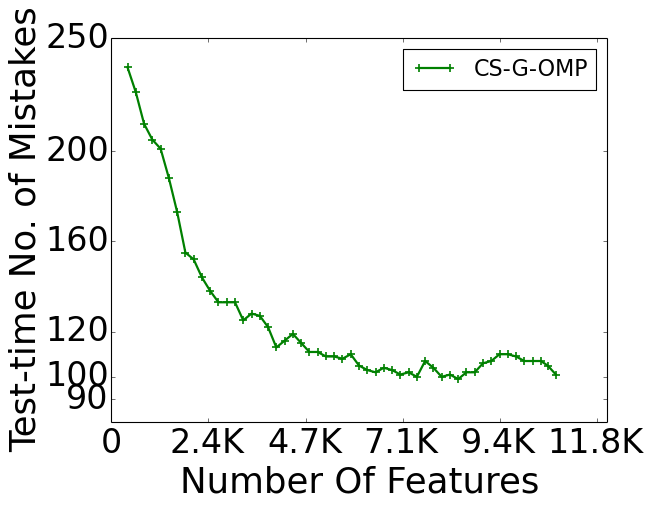
\includegraphics[width=0.3\textwidth]{img/extra_exp_v2.png}
\caption{CS-G-OMP test-time performance on MNIST} 
\label{fig:mnist}
\end{figure}
We present here experimental results of CS-G-OMP with generalized linear models on a MNIST database of handwritten digit classification\cite{MNIST}.
We generate features from raw digit pixels following the recent development of \cite{gem}. It  generates about 11,000 dimensional features via generalized eigenvectors of pairs of second moments of the raw pixel values of different classes, and achieves one-percent error rate with logistic regressions. We partition the generated features into 54 equal-sized random feature groups, and apply CS-G-OMP with multi-class-logistic regression, targeting the one-hot encodings of sample labels. Mathematically, we choose our mean function of generalized linear model, $\nabla \phi: \mathbb{R}^P \rightarrow \mathbb{R}^P$, as $\nabla \phi(x) = \frac{exp(x)}{\sum _p^P exp(x)_p}$ for Algorithm~\ref{algo:gomp_glm}, where $exp(x)$ is an element-wise exponential function. 

As shown in Figure~\ref{fig:mnist}, the test-time accuracy improves greatly at start, quickly reducing the number of mistakes below 150 (i.e., 98.5\% accuracy with the 10K test samples of MNIST) with 2200 out of the 11k total features, and plateaus between 105 and 100 mistakes with 6k features and beyond. The peak performance is 99 mistakes, and the final result has 101 mistakes. We were unable to reproduce results of \cite{gem}, which has 96 mistakes, possibly because of feature generation parameter tuning. Since logistic regression with 11K features and 60K training samples takes non-trivial time to train, the runtime gap between CS-G-OMP and CS-G-FR further widens: CS-G-OMP is able to finish the sequencing in 12 hours, while CS-G-FR takes days to progress. This is because the model training time is orders of magnitudes longer than that of computing gradient w.r.t. the coefficient matrix. In fact, one selection of CS-G-FR takes longer than the full run of CS-G-OMP. As a result, we do not report CS-G-FR result on this data-set.






%\bibliographystyle{plainnat}
%\bibliography{final}
%\end{document}

\chapter{Streaming Gradient Boosting}
%% This is file `elsarticle-template-1-num.tex',
%%
%% Copyright 2009 Elsevier Ltd
%%
%% This file is part of the 'Elsarticle Bundle'.
%% ---------------------------------------------
%%
%% It may be distributed under the conditions of the LaTeX Project Public
%% License, either version 1.2 of this license or (at your option) any
%% later version.  The latest version of this license is in
%%    http://www.latex-project.org/lppl.txt
%% and version 1.2 or later is part of all distributions of LaTeX
%% version 1999/12/01 or later.
%%
%% Template article for Elsevier's document class `elsarticle'
%% with numbered style bibliographic references
%%
%% $Id: elsarticle-template-1-num.tex 149 2009-10-08 05:01:15Z rishi $
%% $URL: http://lenova.river-valley.com/svn/elsbst/trunk/elsarticle-template-1-num.tex $
%%
\documentclass[preprint,12pt]{elsarticle}
\frenchspacing 
\setlength{\pdfpagewidth}{8.5in}
\setlength{\pdfpageheight}{11in}

%% Use the option review to obtain double line spacing
%% \documentclass[preprint,review,12pt]{elsarticle}

%% Use the options 1p,twocolumn; 3p; 3p,twocolumn; 5p; or 5p,twocolumn
%% for a journal layout:
%% \documentclass[final,1p,times]{elsarticle}
%% \documentclass[final,1p,times,twocolumn]{elsarticle}
%% \documentclass[final,3p,times]{elsarticle}
%% \documentclass[final,3p,times,twocolumn]{elsarticle}
%% \documentclass[final,5p,times]{elsarticle}
%% \documentclass[final,5p,times,twocolumn]{elsarticle}

%% The graphicx package provides the includegraphics command.
\usepackage{graphicx}
%% The amssymb package provides various useful mathematical symbols
\usepackage{amssymb}
%% The amsthm package provides extended theorem environments
%% \usepackage{amsthm}

%% The lineno packages adds line numbers. Start line numbering with
%% \begin{linenumbers}, end it with \end{linenumbers}. Or switch it on
%% for the whole article with \linenumbers after \end{frontmatter}.
\usepackage{lineno}

% Set the typeface to Times Roman
\usepackage{times}

\usepackage{hyperref}
\usepackage{url}
\usepackage{natbib}
\usepackage{epsfig}
\usepackage{microtype}
\usepackage{amsmath}
\usepackage{amssymb}
\usepackage{amsthm}

\usepackage{bbold}
\usepackage{flushend}
\usepackage{subfig}
\usepackage{array}
\usepackage{comment}
\usepackage{subfig}
\usepackage{longtable}
\usepackage{hhline}
\usepackage{helvet}
\usepackage{courier}

\usepackage[final]{pdfpages}

\usepackage{enumitem}

%\usepackage[ruled,vlined,linesnumbered,resetcount]{algorithm2e}

\usepackage{booktabs}       % professional-quality tables
\usepackage{amsfonts}       % blackboard math symbols
%\usepackage{nicefrac}       % compact symbols for 1/2, etc.
\usepackage{microtype}      % microtypography
\usepackage{algorithm}
\usepackage{algorithmic}

\usepackage{caption}
%\usepackage{subcaption}
\usepackage{xspace}
\usepackage{color}

\usepackage{amsthm}
\usepackage{natbib}
\setcitestyle{authoryear,open={(},close={)}}
\usepackage{bbm}
\usepackage{multirow}



%\newtheorem{theorem}{Theorem}[section]
%\newtheorem{lemma}[theorem]{Lemma}
%
%\theoremstyle{definition}
%\newtheorem{definition}[theorem]{Definition}
%\newtheorem{example}[theorem]{Example}
%\newtheorem{xca}[theorem]{Exercise}

%\theoremstyle{remark}
%\newtheorem{remark}[theorem]{Remark}

\newcommand{\E}{\mathbb{E}}
\newcommand{\R}{\mathbb{R}}
\newcommand{\angleb}[1]{\langle #1 \rangle}

\newcommand{\at}[1]{\langle #1 \rangle}
\newcommand{\XX}{\textbf{X}}
\newcommand{\YY}{\textbf{Y}}


\makeatletter
\newtheorem*{rep@theorem}{\rep@title}
\newcommand{\newreptheorem}[2]{%
\newenvironment{rep#1}[1]{%
 \def\rep@title{#2 \ref{##1}}%
 \begin{rep@theorem}}%
 {\end{rep@theorem}}}
\makeatother

\newcommand{\defmu}{}
\newcommand{\innerprod}[3][\defmu]{{\left\langle {#2},{#3} \right\rangle}_{#1}}
\newcommand{\norm}[2][\defmu]{{\left\lVert {#2} \right\rVert}_{#1}}
\newcommand{\functional}[3][\defmu]{{\mathcal{#2}}_{#1} [#3]}
\newcommand{\risk}[2][\defmu]{\functional[#1]{R}{#2}}

\newreptheorem{theorem}{Theorem}
\newreptheorem{definition}{Definition}


\newtheorem{theorem}{Theorem}[section]
\newtheorem{lemma}[theorem]{Lemma}
\newtheorem{proposition}[theorem]{Proposition}
\newtheorem{corollary}[theorem]{Corollary}
\newtheorem{definition}[theorem]{Definition}
\newtheorem{assumption}[theorem]{Assumption}
\newenvironment{myproof}[1][\proofname]{\proof[#1]\mbox{}}{\endproof}
 
\newcommand{\algname}{Streaming Gradient Boosting\xspace}
\newcommand{\algshort}{SGB\xspace}
\newcommand{\algnospace}{SGB} 





\setcounter{secnumdepth}{5}


\newcommand{\fix}{\marginpar{FIX}}
\newcommand{\new}{\marginpar{NEW}}
\newcommand{\YahooDataset}{Yahoo! Learning to Rank Challenge dataset}
\newcommand{\YahooLTR}{\textsc{Yahoo!\,LTR}}
\newcommand{\GrainDataset}{Agricultural dataset}
\newcommand{\Grain}{\textsc{Agricultural}}


\newcommand{\annnames}{Anytime Neural Networks\xspace}
\newcommand{\annname}{Anytime Neural Network\xspace}
\newcommand{\ann}{ANN\xspace}
\newcommand{\annnp}{ANN} 
\newcommand{\anns}{ANNs\xspace}
\newcommand{\aannnp}{AANN}
\newcommand{\aann}{AANN\xspace}
\newcommand{\aanns}{AANNs\xspace}
\newcommand{\adaloss}{AdaLoss\xspace}
\newcommand{\sieve}{SIEVE\xspace}
\newcommand{\explin}{EXP-LIN\xspace}
\newcommand{\const}{CONST\xspace}
\newcommand{\linear}{LINEAR\xspace}
\newcommand{\round}[1]{\lfloor #1 \rceil}

% petridish
\newcommand{\stopforward}{\textrm{sf}}
\newcommand{\stopgradient}{\textrm{sg}}
\newcommand{\petridishhard}{Isolated\xspace}
\newcommand{\petridishsoft}{Joint\xspace}
\newcommand{\Petridish}{Petridish\xspace}
\newcommand{\PetridishCP}{Petridish-CP\xspace}
\newcommand{\PetridishWS}{Petridish-WS\xspace}



\DeclareMathOperator*{\argmax}{arg\,max} 
\DeclareMathOperator*{\argmin}{arg\,min}

\allowdisplaybreaks



\newcommand{\GOMPDIR}{1_gomp}
\newcommand{\SGBDIR}{2_sgb}
\newcommand{\ANNDIR}{3_ann}
\newcommand{\NASDIR}{4_nas}



%% natbib.sty is loaded by default. However, natbib options can be
%% provided with \biboptions{...} command. Following options are
%% valid:

%%   round  -  round parentheses are used (default)
%%   square -  square brackets are used   [option]
%%   curly  -  curly braces are used      {option}
%%   angle  -  angle brackets are used    <option>
%%   semicolon  -  multiple citations separated by semi-colon
%%   colon  - same as semicolon, an earlier confusion
%%   comma  -  separated by comma
%%   numbers-  selects numerical citations
%%   super  -  numerical citations as superscripts
%%   sort   -  sorts multiple citations according to order in ref. list
%%   sort&compress   -  like sort, but also compresses numerical citations
%%   compress - compresses without sorting
%%
%% \biboptions{comma,round}

% \biboptions{}

\journal{Journal Name}

\begin{document}

\begin{frontmatter}

%% Title, authors and addresses

\title{Unnecessarily Complicated Research Title}

%% use the tnoteref command within \title for footnotes;
%% use the tnotetext command for the associated footnote;
%% use the fnref command within \author or \address for footnotes;
%% use the fntext command for the associated footnote;
%% use the corref command within \author for corresponding author footnotes;
%% use the cortext command for the associated footnote;
%% use the ead command for the email address,
%% and the form \ead[url] for the home page:
%%
%% \title{Title\tnoteref{label1}}
%% \tnotetext[label1]{}
%% \author{Name\corref{cor1}\fnref{label2}}
%% \ead{email address}
%% \ead[url]{home page}
%% \fntext[label2]{}
%% \cortext[cor1]{}
%% \address{Address\fnref{label3}}
%% \fntext[label3]{}


%% use optional labels to link authors explicitly to addresses:
%% \author[label1,label2]{<author name>}
%% \address[label1]{<address>}
%% \address[label2]{<address>}

\author{John Smith}

\address{California, United States}

\begin{abstract}
%% Text of abstract
Suspendisse potenti. Suspendisse quis sem elit, et mattis nisl. Phasellus consequat erat eu velit rhoncus non pharetra neque auctor. Phasellus eu lacus quam. Ut ipsum dolor, euismod aliquam congue sed, lobortis et orci. Mauris eget velit id arcu ultricies auctor in eget dolor. Pellentesque suscipit adipiscing sem, imperdiet laoreet dolor elementum ut. Mauris condimentum est sed velit lacinia placerat. Vestibulum ante ipsum primis in faucibus orci luctus et ultrices posuere cubilia Curae; Nullam diam metus, pharetra vitae euismod sed, placerat ultrices eros. Aliquam tincidunt dapibus venenatis. In interdum tellus nec justo accumsan aliquam. Nulla sit amet massa augue.
\end{abstract}

\begin{keyword}
Science \sep Publication \sep Complicated
%% keywords here, in the form: keyword \sep keyword

%% MSC codes here, in the form: \MSC code \sep code
%% or \MSC[2008] code \sep code (2000 is the default)

\end{keyword}

\end{frontmatter}

%%
%% Start line numbering here if you want
%%
\linenumbers

\chapter{Anytime Linear Prediction}
%
%\documentclass[]{article}
%
%% Set the typeface to Times Roman
%\usepackage{times}
%
%\usepackage{../styles/uai20162e}
%\usepackage{hyperref}
%\usepackage{url}
%
%\usepackage{natbib}
%\usepackage{epsfig}
%\usepackage{graphicx}
%\usepackage{amsmath}
%\usepackage{amssymb}
%\usepackage{amsthm}
%\usepackage{bbold}
%\usepackage{flushend}
%\usepackage{subfig}
%\usepackage{array}
%\usepackage{comment}
%\usepackage{subfig}
%
%\usepackage[final]{pdfpages}
%
%\usepackage{enumitem}
%
%\usepackage[ruled,vlined,linesnumbered,resetcount]{algorithm2e}
%
%\newtheorem{theorem}{Theorem}[section]
%\newtheorem{lemma}[theorem]{Lemma}
%
%\theoremstyle{definition}
%\newtheorem{definition}[theorem]{Definition}
%\newtheorem{example}[theorem]{Example}
%\newtheorem{xca}[theorem]{Exercise}
%
%\theoremstyle{remark}
%\newtheorem{remark}[theorem]{Remark}
%
%\newcommand{\E}{\mathbb{E}}
%\newcommand{\R}{\mathbb{R}}
%\newcommand{\angleb}[1]{\langle #1 \rangle}
%
%\newcommand{\at}[1]{\langle #1 \rangle}
%\newcommand{\XX}{\textbf{X}}
%\newcommand{\YY}{\textbf{Y}}
%
%\setcounter{secnumdepth}{5}
%
%
%\newcommand{\fix}{\marginpar{FIX}}
%\newcommand{\new}{\marginpar{NEW}}
%\newcommand{\YahooDataset}{Yahoo! Learning to Rank Challenge dataset}
%\newcommand{\YahooLTR}{\textsc{Yahoo!\,LTR}}
%\newcommand{\GrainDataset}{Agricultural dataset}
%\newcommand{\Grain}{\textsc{Agricultural}}
%
%\DeclareMathOperator*{\argmax}{argmax} 
%
%\allowdisplaybreaks
%
%%\nipsfinalcopy % Uncomment for camera-ready version
%%\runningauthor{Surname 1, Surname 2, Surname 3, ...., Surname n}
%
%
%
%\title{Efficient Feature Group Sequencing for 
%Anytime Linear Prediction}
%
%%\aistatsauthor{ Hanzhang Hu \And Alexander Grubb \And J. Andrew Bagnell \And Martial Hebert}
%
%%\aistatsaddress{hanzhang@andrew.cmu.edu \And agrubb@cmu.edu \And dbagnell@ri.cmu.edu \And hebert@ri.cmu.edu } 
%
%\author{ {\bf Hanzhang Hu} \\
%hanzhang@cs.cmu.edu \\
%\And
%{\bf Alexander Grubb}  \\
%agrubb@cs.cmu.edu \\
%\And
%{\bf J. Andrew Bagnell}   \\
%dbagnell@ri.cmu.edu \\
%\And
%{\bf Martial Hebert} \\
%hebert@ri.cmu.edu
%}
%
%\begin{document}
%
%\maketitle
%

%\input{\GOMPDIR/0_abstract}

\input{\GOMPDIR/1_introduction.tex}

% Define the problem of feature group sequencing for linear prediction anytime
% - mathematical form; 
% - anytime;
% - mathematical guarantee target; (what we have in theorem)
% - meaning; - example; 


% background 
% - relation to feature selection; (different assumption)
% - relation to submodular maximization; (different/stronger bound; bound specific to group feature of varied cost) 


% Define contribution: 
% - anytime prediction (linear predictors, sequence the features) 
% - theoretic guarantee (stronger), specific to group setting
% - extension to generalized linear model. 
% - 

\input{\GOMPDIR/2_method.tex}

% Algorithm description. 

\input{\GOMPDIR/3_proof.tex}

% terms, assumption, lemma
% Proof of the main lemma;

\input{\GOMPDIR/5_experiment.tex}


\input{\GOMPDIR/3_proof_II.tex}
\input{\GOMPDIR/4_extension.tex}
\input{\GOMPDIR/7_extra_exp.tex}

%\bibliographystyle{plainnat}
%\bibliography{final}
%\end{document}

\chapter{Streaming Gradient Boosting}
%% This is file `elsarticle-template-1-num.tex',
%%
%% Copyright 2009 Elsevier Ltd
%%
%% This file is part of the 'Elsarticle Bundle'.
%% ---------------------------------------------
%%
%% It may be distributed under the conditions of the LaTeX Project Public
%% License, either version 1.2 of this license or (at your option) any
%% later version.  The latest version of this license is in
%%    http://www.latex-project.org/lppl.txt
%% and version 1.2 or later is part of all distributions of LaTeX
%% version 1999/12/01 or later.
%%
%% Template article for Elsevier's document class `elsarticle'
%% with numbered style bibliographic references
%%
%% $Id: elsarticle-template-1-num.tex 149 2009-10-08 05:01:15Z rishi $
%% $URL: http://lenova.river-valley.com/svn/elsbst/trunk/elsarticle-template-1-num.tex $
%%
\documentclass[preprint,12pt]{elsarticle}
\frenchspacing 
\setlength{\pdfpagewidth}{8.5in}
\setlength{\pdfpageheight}{11in}

%% Use the option review to obtain double line spacing
%% \documentclass[preprint,review,12pt]{elsarticle}

%% Use the options 1p,twocolumn; 3p; 3p,twocolumn; 5p; or 5p,twocolumn
%% for a journal layout:
%% \documentclass[final,1p,times]{elsarticle}
%% \documentclass[final,1p,times,twocolumn]{elsarticle}
%% \documentclass[final,3p,times]{elsarticle}
%% \documentclass[final,3p,times,twocolumn]{elsarticle}
%% \documentclass[final,5p,times]{elsarticle}
%% \documentclass[final,5p,times,twocolumn]{elsarticle}

%% The graphicx package provides the includegraphics command.
\usepackage{graphicx}
%% The amssymb package provides various useful mathematical symbols
\usepackage{amssymb}
%% The amsthm package provides extended theorem environments
%% \usepackage{amsthm}

%% The lineno packages adds line numbers. Start line numbering with
%% \begin{linenumbers}, end it with \end{linenumbers}. Or switch it on
%% for the whole article with \linenumbers after \end{frontmatter}.
\usepackage{lineno}

% Set the typeface to Times Roman
\usepackage{times}

\usepackage{hyperref}
\usepackage{url}
\usepackage{natbib}
\usepackage{epsfig}
\usepackage{microtype}
\usepackage{amsmath}
\usepackage{amssymb}
\usepackage{amsthm}

\usepackage{bbold}
\usepackage{flushend}
\usepackage{subfig}
\usepackage{array}
\usepackage{comment}
\usepackage{subfig}
\usepackage{longtable}
\usepackage{hhline}
\usepackage{helvet}
\usepackage{courier}

\usepackage[final]{pdfpages}

\usepackage{enumitem}

%\usepackage[ruled,vlined,linesnumbered,resetcount]{algorithm2e}

\usepackage{booktabs}       % professional-quality tables
\usepackage{amsfonts}       % blackboard math symbols
%\usepackage{nicefrac}       % compact symbols for 1/2, etc.
\usepackage{microtype}      % microtypography
\usepackage{algorithm}
\usepackage{algorithmic}

\usepackage{caption}
%\usepackage{subcaption}
\usepackage{xspace}
\usepackage{color}

\usepackage{amsthm}
\usepackage{natbib}
\setcitestyle{authoryear,open={(},close={)}}
\usepackage{bbm}
\usepackage{multirow}



%\newtheorem{theorem}{Theorem}[section]
%\newtheorem{lemma}[theorem]{Lemma}
%
%\theoremstyle{definition}
%\newtheorem{definition}[theorem]{Definition}
%\newtheorem{example}[theorem]{Example}
%\newtheorem{xca}[theorem]{Exercise}

%\theoremstyle{remark}
%\newtheorem{remark}[theorem]{Remark}

\newcommand{\E}{\mathbb{E}}
\newcommand{\R}{\mathbb{R}}
\newcommand{\angleb}[1]{\langle #1 \rangle}

\newcommand{\at}[1]{\langle #1 \rangle}
\newcommand{\XX}{\textbf{X}}
\newcommand{\YY}{\textbf{Y}}


\makeatletter
\newtheorem*{rep@theorem}{\rep@title}
\newcommand{\newreptheorem}[2]{%
\newenvironment{rep#1}[1]{%
 \def\rep@title{#2 \ref{##1}}%
 \begin{rep@theorem}}%
 {\end{rep@theorem}}}
\makeatother

\newcommand{\defmu}{}
\newcommand{\innerprod}[3][\defmu]{{\left\langle {#2},{#3} \right\rangle}_{#1}}
\newcommand{\norm}[2][\defmu]{{\left\lVert {#2} \right\rVert}_{#1}}
\newcommand{\functional}[3][\defmu]{{\mathcal{#2}}_{#1} [#3]}
\newcommand{\risk}[2][\defmu]{\functional[#1]{R}{#2}}

\newreptheorem{theorem}{Theorem}
\newreptheorem{definition}{Definition}


\newtheorem{theorem}{Theorem}[section]
\newtheorem{lemma}[theorem]{Lemma}
\newtheorem{proposition}[theorem]{Proposition}
\newtheorem{corollary}[theorem]{Corollary}
\newtheorem{definition}[theorem]{Definition}
\newtheorem{assumption}[theorem]{Assumption}
\newenvironment{myproof}[1][\proofname]{\proof[#1]\mbox{}}{\endproof}
 
\newcommand{\algname}{Streaming Gradient Boosting\xspace}
\newcommand{\algshort}{SGB\xspace}
\newcommand{\algnospace}{SGB} 





\setcounter{secnumdepth}{5}


\newcommand{\fix}{\marginpar{FIX}}
\newcommand{\new}{\marginpar{NEW}}
\newcommand{\YahooDataset}{Yahoo! Learning to Rank Challenge dataset}
\newcommand{\YahooLTR}{\textsc{Yahoo!\,LTR}}
\newcommand{\GrainDataset}{Agricultural dataset}
\newcommand{\Grain}{\textsc{Agricultural}}


\newcommand{\annnames}{Anytime Neural Networks\xspace}
\newcommand{\annname}{Anytime Neural Network\xspace}
\newcommand{\ann}{ANN\xspace}
\newcommand{\annnp}{ANN} 
\newcommand{\anns}{ANNs\xspace}
\newcommand{\aannnp}{AANN}
\newcommand{\aann}{AANN\xspace}
\newcommand{\aanns}{AANNs\xspace}
\newcommand{\adaloss}{AdaLoss\xspace}
\newcommand{\sieve}{SIEVE\xspace}
\newcommand{\explin}{EXP-LIN\xspace}
\newcommand{\const}{CONST\xspace}
\newcommand{\linear}{LINEAR\xspace}
\newcommand{\round}[1]{\lfloor #1 \rceil}

% petridish
\newcommand{\stopforward}{\textrm{sf}}
\newcommand{\stopgradient}{\textrm{sg}}
\newcommand{\petridishhard}{Isolated\xspace}
\newcommand{\petridishsoft}{Joint\xspace}
\newcommand{\Petridish}{Petridish\xspace}
\newcommand{\PetridishCP}{Petridish-CP\xspace}
\newcommand{\PetridishWS}{Petridish-WS\xspace}



\DeclareMathOperator*{\argmax}{arg\,max} 
\DeclareMathOperator*{\argmin}{arg\,min}

\allowdisplaybreaks



\newcommand{\GOMPDIR}{1_gomp}
\newcommand{\SGBDIR}{2_sgb}
\newcommand{\ANNDIR}{3_ann}
\newcommand{\NASDIR}{4_nas}



%% natbib.sty is loaded by default. However, natbib options can be
%% provided with \biboptions{...} command. Following options are
%% valid:

%%   round  -  round parentheses are used (default)
%%   square -  square brackets are used   [option]
%%   curly  -  curly braces are used      {option}
%%   angle  -  angle brackets are used    <option>
%%   semicolon  -  multiple citations separated by semi-colon
%%   colon  - same as semicolon, an earlier confusion
%%   comma  -  separated by comma
%%   numbers-  selects numerical citations
%%   super  -  numerical citations as superscripts
%%   sort   -  sorts multiple citations according to order in ref. list
%%   sort&compress   -  like sort, but also compresses numerical citations
%%   compress - compresses without sorting
%%
%% \biboptions{comma,round}

% \biboptions{}

\journal{Journal Name}

\begin{document}

\begin{frontmatter}

%% Title, authors and addresses

\title{Unnecessarily Complicated Research Title}

%% use the tnoteref command within \title for footnotes;
%% use the tnotetext command for the associated footnote;
%% use the fnref command within \author or \address for footnotes;
%% use the fntext command for the associated footnote;
%% use the corref command within \author for corresponding author footnotes;
%% use the cortext command for the associated footnote;
%% use the ead command for the email address,
%% and the form \ead[url] for the home page:
%%
%% \title{Title\tnoteref{label1}}
%% \tnotetext[label1]{}
%% \author{Name\corref{cor1}\fnref{label2}}
%% \ead{email address}
%% \ead[url]{home page}
%% \fntext[label2]{}
%% \cortext[cor1]{}
%% \address{Address\fnref{label3}}
%% \fntext[label3]{}


%% use optional labels to link authors explicitly to addresses:
%% \author[label1,label2]{<author name>}
%% \address[label1]{<address>}
%% \address[label2]{<address>}

\author{John Smith}

\address{California, United States}

\begin{abstract}
%% Text of abstract
Suspendisse potenti. Suspendisse quis sem elit, et mattis nisl. Phasellus consequat erat eu velit rhoncus non pharetra neque auctor. Phasellus eu lacus quam. Ut ipsum dolor, euismod aliquam congue sed, lobortis et orci. Mauris eget velit id arcu ultricies auctor in eget dolor. Pellentesque suscipit adipiscing sem, imperdiet laoreet dolor elementum ut. Mauris condimentum est sed velit lacinia placerat. Vestibulum ante ipsum primis in faucibus orci luctus et ultrices posuere cubilia Curae; Nullam diam metus, pharetra vitae euismod sed, placerat ultrices eros. Aliquam tincidunt dapibus venenatis. In interdum tellus nec justo accumsan aliquam. Nulla sit amet massa augue.
\end{abstract}

\begin{keyword}
Science \sep Publication \sep Complicated
%% keywords here, in the form: keyword \sep keyword

%% MSC codes here, in the form: \MSC code \sep code
%% or \MSC[2008] code \sep code (2000 is the default)

\end{keyword}

\end{frontmatter}

%%
%% Start line numbering here if you want
%%
\linenumbers

\chapter{Anytime Linear Prediction}
\input{\GOMPDIR/final.tex}
\chapter{Streaming Gradient Boosting}
\input{\SGBDIR/main.tex}
\chapter{Anytime Neural Network}
\input{\ANNDIR/AAAI-HuH.2508.tex}
\chapter{Neural Network Search}
\input{\NASDIR/main_conference.tex}


%% The Appendices part is started with the command \appendix;
%% appendix sections are then done as normal sections
%% \appendix

%% \section{}
%% \label{}

%% References
%%
%% Following citation commands can be used in the body text:
%% Usage of \cite is as follows:
%%   \cite{key}          ==>>  [#]
%%   \cite[chap. 2]{key} ==>>  [#, chap. 2]
%%   \citet{key}         ==>>  Author [#]

%% References with bibTeX database:

\bibliographystyle{natbib}
\bibliography{1_gomp/final.bib}

%% Authors are advised to submit their bibtex database files. They are
%% requested to list a bibtex style file in the manuscript if they do
%% not want to use model1-num-names.bst.

%% References without bibTeX database:

% \begin{thebibliography}{00}

%% \bibitem must have the following form:
%%   \bibitem{key}...
%%

% \bibitem{}

% \end{thebibliography}


\end{document}

%%
%% End of file `elsarticle-template-1-num.tex'.

\chapter{Anytime Neural Network}
%\def\year{2019}\relax
%\documentclass[letterpaper]{article}
%\usepackage{aaai19}
%\usepackage{times}
%\usepackage{helvet}
%\usepackage{courier}
%\usepackage{url}
%\usepackage{graphicx}
%\frenchspacing 
%\setlength{\pdfpagewidth}{8.5in}
%\setlength{\pdfpageheight}{11in}
%\setcounter{secnumdepth}{2} 
%
%%PDF Info Is Required:
%  \pdfinfo{
%/Title (Learning Anytime Predictions in Neural Networks via Adaptive Loss Balancing)
%/Author (Hanzhang Hu, Debadeepta Dey, Martial Hebert, J. Andrew Bagnell)}
%
%\usepackage{subfig}
%\usepackage{xspace}
%\usepackage{color}
%\usepackage{longtable}
%\usepackage{hhline}
%
%% For algorithms
%\usepackage{algorithm}
%\usepackage{algorithmic}
%
%
%% Employ the following version of the ``usepackage'' statement for
%% submitting the draft version of the paper for review.  This will set
%% the note in the first column to ``Under review.  Do not distribute.''
%
%%\usepackage{fancyhdr}		% allows headers and footers
%%\usepackage{lastpage}		% provides page number of last page
%
%\usepackage{amsmath}
%\usepackage{amssymb}
%\usepackage{amsthm}
%
%\makeatletter
%\newtheorem*{rep@theorem}{\rep@title}
%\newcommand{\newreptheorem}[2]{%
%\newenvironment{rep#1}[1]{%
% \def\rep@title{#2 \ref{##1}}%
% \begin{rep@theorem}}%
% {\end{rep@theorem}}}
%\makeatother
%
%\newreptheorem{theorem}{Theorem}
%\newreptheorem{definition}{Definition}
%
%
%\newtheorem{theorem}{Theorem}[section]
%\newtheorem{lemma}[theorem]{Lemma}
%\newtheorem{proposition}[theorem]{Proposition}
%\newtheorem{corollary}[theorem]{Corollary}
%\newtheorem{definition}[theorem]{Definition}
%\newtheorem{assumption}[theorem]{Assumption}
%\newenvironment{myproof}[1][\proofname]{\proof[#1]\mbox{}}{\endproof}
%
%\newcommand{\annnames}{Anytime Neural Networks\xspace}
%\newcommand{\annname}{Anytime Neural Network\xspace}
%\newcommand{\ann}{ANN\xspace}
%\newcommand{\annnp}{ANN} 
%\newcommand{\anns}{ANNs\xspace}
%\newcommand{\aannnp}{AANN}
%\newcommand{\aann}{AANN\xspace}
%\newcommand{\aanns}{AANNs\xspace}
%\newcommand{\adaloss}{AdaLoss\xspace}
%\newcommand{\sieve}{SIEVE\xspace}
%\newcommand{\explin}{EXP-LIN\xspace}
%\newcommand{\const}{CONST\xspace}
%\newcommand{\linear}{LINEAR\xspace}
%\newcommand{\round}[1]{\lfloor #1 \rceil}
%
%\title{Learning Anytime Predictions in Neural Networks  
%via Adaptive Loss Balancing  }
%
%\author{
%Hanzhang Hu,\textsuperscript{\rm 1}
%Debadeepta Dey,\textsuperscript{\rm 2}
%Martial Hebert,\textsuperscript{\rm 1}
%J. Andrew Bagnell\textsuperscript{\rm 1}\\
%\textsuperscript{\rm 1}Carnegie Mellon University,
%\textsuperscript{\rm 2}Microsoft Research\\
%hanzhang@cs.cmu.edu, dedey@microsoft.com, hebert@cs.cmu.edu, dbagnell@cs.cmu.edu
%}
%
%
%\begin{document}
%\maketitle
%\begin{abstract}
%This work considers the trade-off between accuracy and test-time computational cost of deep neural networks (DNNs) via \emph{anytime} predictions from auxiliary predictions. Specifically, we optimize auxiliary losses jointly in an \emph{adaptive} weighted sum, where the weights are inversely proportional to average of each loss. 
%Intuitively, this balances the losses to have the same scale.
%We demonstrate theoretical considerations that motivate this approach from multiple viewpoints, including connecting it to optimizing the geometric mean of the expectation of each loss, an objective that ignores the scale of losses. 
%Experimentally, the adaptive weights induce more competitive anytime predictions on multiple recognition data-sets and models than non-adaptive approaches including weighing all losses equally. In particular, anytime neural networks (\anns) can achieve the same accuracy faster using adaptive weights on a small network than using static constant weights on a large one.
%For problems with high performance saturation, we also show a sequence of exponentially deepening \anns can achieve near-optimal anytime results at any budget, at the cost of a const fraction of extra computation. 
%\end{abstract}
%
%

\section{Introduction}
\label{sec:introduction}

Recent years have seen advancement in visual recognition tasks
by increasingly accurate convolutional neural networks, from AlexNet~\cite{alexnet} and VGG~\cite{vgg}, to ResNet~\cite{resnet}, ResNeXt~\cite{resnext}, and DenseNet~\cite{densenet}. 
As models become more accurate and computationally expensive, it becomes more difficult for applications to choose between slow predictors with high accuracy and fast predictors with low accuracy. 
Some applications also desire multiple trade-offs between computation and accuracy, because they have computational budgets that may vary at test time. E.g., web servers for facial recognition or spam filtering may have higher load during the afternoon than at midnight.  Autonomous vehicles need faster object detection when moving rapidly than when it is stationary.  Furthermore, real-time and latency sensitive applications may desire fast predictions on easy samples and slow but accurate predictions on difficult ones. 
\begin{figure}
    \centering
    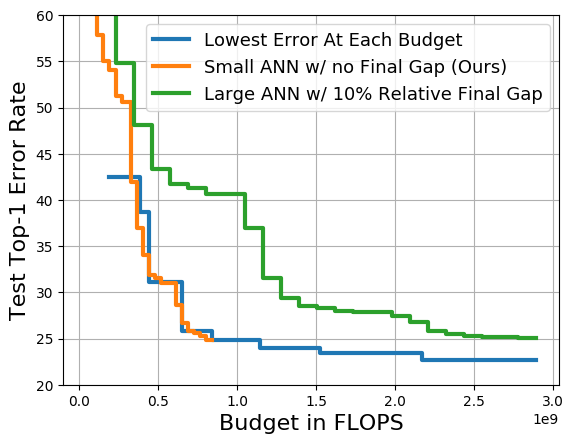
\includegraphics[width=0.85\linewidth, keepaspectratio]{\ANNDIR/adaloss_small_vs_const_large.png}
    \caption{The common \ann training strategy increases final errors from the optimal (green vs. blue), which decreases exponentially slowly. By learning to focus more on the final auxiliary losses, the proposed adaptive loss weights make a small \ann (orange) to outperform a large one (green) that has non-adaptive weights. }
    \label{fig:sieve_small_vs_const_large}
\end{figure}

An \textbf{anytime predictor}~\cite{horvitz:1987,boddydean,anytime,speedboost,msdense} can automatically trade off between computation and accuracy. For each test sample, an anytime predictor produces a fast and crude initial prediction and continues to refine it as budget allows, so that at any test-time budget, the anytime predictor has a valid result for the sample, and the more budget is spent, the better the prediction. 
Anytime predictors are different from cascaded predictors~\cite{cascade,xu:14,cai:15,adaptivenn,cascade_nn} for \textbf{budgeted prediction}, which aim to minimize \textbf{average test-time computational cost} without sacrificing average accuracy: a different task (with relation to anytime prediction). Cascades achieve this by early exiting on easy samples to save computation for difficult ones, but cascades cannot incrementally improve individual samples after an exit. Furthermore, early exit policy of cascades can be combined with existing anytime predictors~\cite{adaptivenn,cascade_nn}. Hence, we consider cascades to be orthogonal to anytime predictions.




\begin{figure}
    \centering
    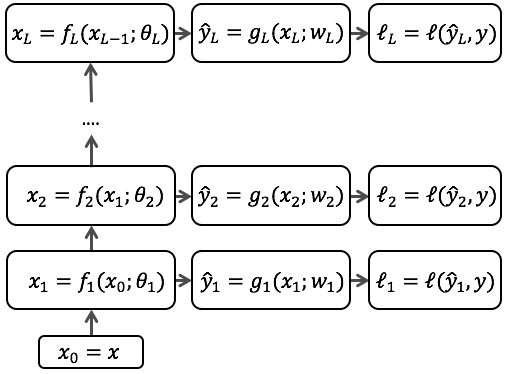
\includegraphics[width=0.85\linewidth, keepaspectratio]{\ANNDIR/ann.png}
    \caption{Anytime neural networks contain auxiliary predictions and losses, $\hat{y}_i$ and $\ell_i$, for intermediate feature unit $f_i$.  }
    \label{fig:ann}
\end{figure}

This work studies how to convert well-known DNN architectures to produce competitive anytime predictions.  
We form anytime neural networks (\anns) by appending auxiliary predictions and losses to DNNs, as we will detail in Sec.~\ref{sec:ann} and Fig.~\ref{fig:ann}. Inference-time prediction then can be stopped at the latest prediction layer that is within the budget. Note that this work deals with the case where it is \textbf{not known apriori} where the interrupt during inference time will occur. 
We define the optimal at each auxiliary loss as the result from training the \ann only for that loss to convergence. Then our objective is to have near-optimal final predictions and competitive early ones.  Near-optimal final accuracy is imperative for anytime predictors, because, as demonstrated in Fig.~\ref{fig:sieve_small_vs_const_large}, accuracy gains are often exponentially more expensive as model sizes grow, so that reducing 1\% error rate could take 50\% extra computation. Unfortunately, existing anytime predictors often optimize the anytime losses in static weighted sums~\cite{supervisednet,feedbacknet,msdense} that poorly optimize final predictions, as we will show in Sec.~\ref{sec:multi_objective} and Sec.~\ref{sec:experiment_questions}.

Instead, we optimize the losses in an \textbf{adaptive} weighted sum, where the weight of a loss is inversely proportional to the empirical mean of the loss on the training set. Intuitively, this normalizes losses to have the same scale, so that the optimization leads each loss to be about the same relative to its optimal. We provide multiple theoretical considerations to motivate such weights.
First of all, when the losses are mean square errors, our approach is maximizing the likelihood of a model where the prediction targets have Gaussian noises. Secondly, inspired by the maximum likelihood estimation, we optimize the model parameters and the loss weights jointly, with log-barriers on the weights to avoid the trivial solution of zero weights. Finally, we find the joint optimization equivalent to optimizing the geometric mean of the expected training losses, an objective that treats the relative improvement of each loss equally. Empirically, we show on multiple models and visual recognition data-sets that the proposed adaptive weights outperform natural, non-adaptive weighting schemes as follows.
We compare small \anns using our adaptive weights against \anns that are $50\sim 100\%$ larger but use non-adaptive weights. The small \anns can reach the same final accuracy as the larger ones, and reach each accuracy level faster.

Early and late accuracy in an \ann are often anti-correlated (e.g., Fig.~7 in~\cite{msdense} shows \anns with better final predictions have worse early ones). To mitigate this \emph{fundamental} issue we propose to assemble \anns of exponentially increasing depths. If \anns are near-optimal in a late fraction of their layers, the exponential ensemble only pays a constant fraction of additional computation to be near-optimal at every test-time budget. In addition, exponential ensembles outperform linear ensembles of networks, which are commonly used baselines for existing works~\cite{feedbacknet,msdense}. 
In summary our contributions are:
\begin{itemize}
    %\item We highlight the importance of near-optimal final predictions in anytime models.
    \item We derive an adaptive weight scheme for training losses in \anns from multiple theoretical considerations, and show that experimentally this scheme achieves near-optimal final accuracy \emph{and} competitive anytime ones on multiple data-sets and models.
    \item We assemble \anns of exponentially increasing depths to achieve near-optimal anytime predictions at every budget at the cost of a constant fraction of additional consumed budget. 
\end{itemize}



\section{Related Works}
\label{sec:background}


\textbf{Meta-algorithms for anytime and budgeted prediction.}
Anytime and budgeted prediction has a rich history in learning literature.
\cite{weinberger09feature,xu:12,xu:13b} sequentially generate features to empower the final predictor.
\cite{reyzin:11,speedboost,hu:16} apply boosting and greedy methods to order feature and predictor computation.  
\cite{timeliness,rl_anytime} form Markov Decision Processes for computation of weak predictors and features, and learn policies to order them. However, these meta-algorithms are not easily compatible with complex and accurate predictors like DNNs, because the anytime predictions without DNNs are inaccurate, and there are no intermediate results during the computation of the DNNs.
Cascade designs for budgeted prediction \cite{cascade,lefakis:10,chen:12,xu:14,cai:15,adaptive_select,adaptivenn,cascade_nn} reduce the average test-time computation by early exiting on easy samples and saving computation for difficult ones. As cascades build upon existing anytime predictors, or combine multiple predictors, they are orthogonal to learning \anns end-to-end.

\textbf{Neural networks with early auxiliary predictions.} 
Multiple works have addressed training DNNs with early auxiliary predictions for various purposes. \cite{supervisednet,inception_v4,pspnet,fractalnet} use them to regularize the networks for faster and better convergence. \cite{curriculum,feedbacknet} set the auxiliary predictions from easy to hard for curriculum learning. \cite{hed,reverse_scene_seg} make pixel level predictions in images, and find learning early predictions in coarse scales also improve the fine resolution predictions. \cite{msdense} shows the crucial importance of maintaining multi-scale features for high quality early classifications. The above works use manually-tuned static weights to combine the auxiliary losses, or change the weights only once~\cite{reverse_scene_seg}. This work proposes adaptive weights to balance the losses to the same scales online, and provides multiple theoretical motivations. We empirically show adaptive losses induce better \anns on multiple models, including the state-of-the-art anytime predictor for image recognition, MSDNet~\cite{msdense}. %There also exist works that train auxiliary losses stage-wise~\cite{boostresnet}, but they suffer from worse accuracy generally. 

\textbf{Model compression.} 
Many  works have studied how to compress neural networks.  \cite{prune_nn,slim_nn} prune network weights and connections. \cite{binary_nn,binary_nn_eccv,squeezenet} quantize weights within networks to reduce computation and memory footprint. 
\cite{wang2017skipnet,veit2017convolutional} dynamically skip network computation based on samples.
\cite{deepreally,distillation} transfer knowledge of deep networks into shallow ones by changing the training target of shallow networks. 
These works are orthogonal to ours, because they train a separate model for each trade-off between computation and accuracy, but we train a single model to handle all possible trade-offs.



%#########################################################
%               Methods
%#########################################################

\section{Optimizing Anytime Predictors}

%\subsection{Training Anytime Neural Networks via Multi-objective Optimization}
\label{sec:ann}

%\subsection{Anytime Augmentation to a Feed-forward Network}
%\label{sec:ann-struct}




%given a sample $(x,y)\sim D$, the initial feature map $x_0$ is set to $x$, and the subsequent feature transformations $f_1, f_2,..., f_L$ generate a sequence of intermediate features $x_i = f_i(x_{i-1} ; \theta_i)$ for $i\geq 1$ using parameter $\theta_i$.  Each feature map $x_i$ can then produce an auxiliary prediction $\hat{y}_i$ using a prediction layer $g_i$: $\hat{y}_i = g_i(x_i; w_i)$ with parameter $w_i$. Each auxiliary prediction $\hat{y}_i$ then incurs an expected loss $\ell_i := E _{(x,y) \sim D} [ \ell( y, \hat{y}_i)]$. We call such an augmented network as an \textit{\annname (\ann)}. 


%For instance, if we base ANNs on ResNets \cite{resnet}, then each $f_i$ contains $s$ number of residual building blocks (whose implementation details are deferred to the appendix), where $s$ is the prediction period. Each $g_i$ outputs the predicted label distribution $\hat{y}_i$ using a global pooling layer followed by a linear layer and a softmax; the loss function $\ell$ is the cross-entropy loss.
%During test-time, an \ann computes $\hat{y}_i$ sequentially until interruption from either users or early exit policies. %The above augmentation is general to feed-forward convolutional network as we experiment in Sec.~\ref{sec:other_networks}.  



%since complex neural networks can fit any labeling of the data for our available data-sets \cite{bengio2016}, 
%when the network is highly over-parameterized, it may be reasonable to assume that the sub neural networks of the full network can encode extra information to enable competitive early predictions, and there may exist $\theta$ such that $\ell_i (\theta) \approx \ell_i^*$ for any $i$.  


%Let the parameters of the full \ann be $\theta = (\theta_1, w_1,  ..., \theta_L, w_L)$. Let $\ell^*_i := \min _{\theta} \ell_i(\theta)$ be the optimal loss at the $i^{th}$  prediction. The goal of training an \ann is to find a single $\theta^*$ such that $\ell_i(\theta^*) =\ell^*_i$ for all $i$, i.e., 
%$ \theta^* \in \cap _{i=1}^L \{ x : x = \arg \min _{\theta} \ell _i(\theta) \}. \label{eq:multi-objective}$
% If the above multi-objective optimization can be solved, then there exists a $\theta^*$ such that simultaneously optimizes all $\ell_i$, i.e., $\ell_i(\theta^*) = \ell_i^*$ for any $i$. 


\label{sec:multi_objective}

As illustrated in Fig.~\ref{fig:ann}, a feed-forward network consists of a sequence of transformations $f_1,...,f_L$ of feature maps. Starting with the input feature map $x_0$, each subsequent feature map is generated by $x_i = f_i(x_{i-1})$.  Typical DNNs use the final feature map $x_L$ to produce predictions, and hence require the completion of the whole network for results. Anytime neural networks (\anns) instead introduce auxiliary predictions and losses using the intermediate feature maps $x_1,...,x_{L-1}$, and thus, have early predictions that are improving with computation. 


%%%%%%%%%%%%%%%%%


\textbf{Weighted sum objective.} Let the intermediate predictions be $\hat{y}_i = g_i(x_i)$ for some function $g_i$, and let the corresponding expected loss be $\ell_i = E_{(x_0,y)\sim \mathcal{D}} [\ell(y, \hat{y}_i)]$, where $\mathcal{D}$ is the distribution of the data, and $\ell$ is some loss such as cross-entropy.  Let $\theta$ be the parameter of the \ann, and define the optimal loss at prediction $\hat{y}_i$ to be $\ell_i* = \min _{\theta}  \ell_i(\theta)$. Then the goal of anytime prediction is to seek a universal 
$
    \theta^* \in \cap _{i=1}^L \{ \theta' : \theta' = \arg \min _{\theta} \ell _i(\theta) \}.
    \label{eq:multi-objective}
$
Such an ideal $\theta^*$ does not exist in general as this is a multi-objective optimization, which only has Pareto front, a set containing all solutions such that improving one $\ell_i$ necessitates degrading others. Finding all solutions in the Pareto front for \anns is not practical or useful, since this requires training multiple models, but each \ann only runs one. Hence, following previous works on anytime models~\cite{supervisednet,feedbacknet,msdense}, we optimize the losses in a weighted sum
$
    \min _{\theta} \sum _{i=1}^L B_i \ell_i (\theta),
    \label{eq:sum-objective}
$
where $B_i$ is the weight of the loss $\ell_i$. We call the choices of $B_i$ \textit{weight schemes}. 


%%%%%%%%%%%%%%%%%

\textbf{Static weight schemes.} Previous works often use static weight schemes as part of their formulation. \cite{supervisednet,hed,msdense} use \const scheme that sets $B_i =1$ for all $i$. \cite{feedbacknet} use \linear scheme that sets $B_1$ to $B_L$ to linearly increase from $0.25$ to $1$. However, as we will show in Sec.~\ref{sec:compare_opt}, these static schemes not only cannot adjust weights in a data and model-dependent manner, but also may significantly degrade predictions at later layers.

\begin{figure}
    \centering
        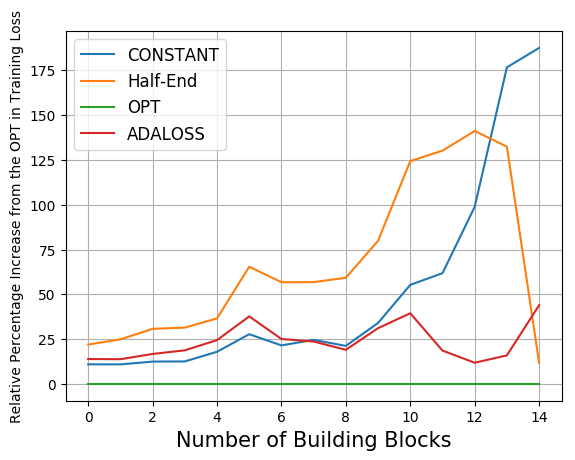
\includegraphics[width=0.80\linewidth, keepaspectratio]{\ANNDIR/loss_cifar100.png}
    \caption{Relative Percentage Increase in Training Loss vs. depths (lower is better). \const scheme is increasingly worse than the optimal at deep layers. \adaloss performs about equally well on all layers in comparison to the OPT.}
    \label{fig:loss_cifar100}
\end{figure}

\begin{figure}
    \centering
    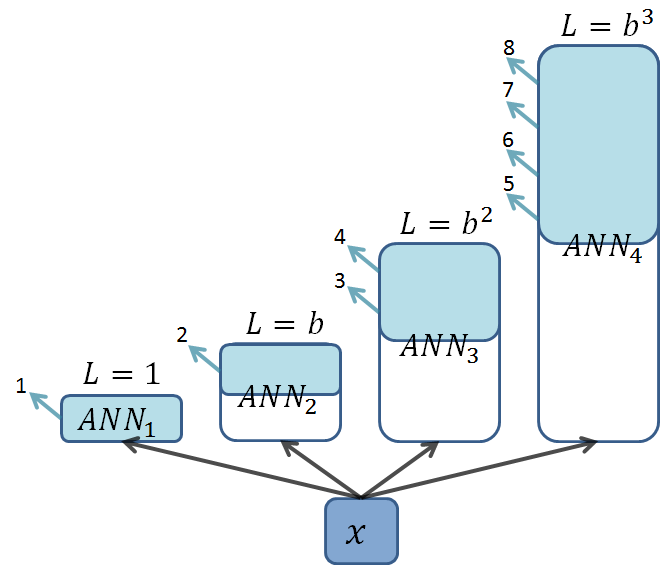
\includegraphics[width=0.75\linewidth, keepaspectratio]{\ANNDIR/EANN.png}
    \caption{ Ensemble of exponentially deepening anytime neural network (EANN) computes its \anns in order of their depths. An anytime result is used if it is better than all previous ones on a validation set (layers in light blue).} 
     \label{fig:eann}
\end{figure}
    %}    
    
%%%%%%%%%%%%%%


\textbf{Qualitative weight scheme comparison.} Before we formally introduce our proposed adaptive weights, we first shed light on how existing static weights suffer. We experiment with a ResNet of 15 basic residual blocks on CIFAR100~\cite{cifar} data-set (See Sec.~\ref{sec:experiment_questions} for data-set details). An anytime predictor is attached to each residual block, and we estimate the optimal performance (OPT) in training cross entropy of predictor $i$ by training a network that has weight only on $\ell_i$ to convergence. Then for each weight scheme we train an \ann to measure the relative increase in training loss at each depth $i$ from the OPT. In Fig.~\ref{fig:loss_cifar100}, we observe that the intuitive \const scheme has high relative losses in late layers. This indicates that there is not enough weights in the late layers, though losses have the same $B_i$.  We also note that balancing the weights is non-trivial. For instance, if we put half of the total weights in the final layer and distribute the other half evenly, we get the ``Half-End" scheme. As expected, the final loss is improved, but this is at the cost of significant increases of early training losses. In contrast, the adaptive weight scheme that we propose next (\adaloss), achieves roughly even relative increases in training losses automatically, and is much better than the \const scheme in the late layers.

%%%%%%%%%%%%%%

\textbf{Adaptive Loss Balancing (\adaloss).} 
% Why the auxiliary losses should have different weights when they are all cross-entropy losses between predictions and the target label? 
Given all losses are of the same form (cross-entropy), it may be surprising
that better performance is achieved with differing weights.
Because early features typically have less predictive power than later ones, early losses are naturally on a larger scale and possess larger gradients. Hence, if we weigh losses equally, early losses and gradients often dominate later ones, and the optimization becomes focused on the early losses.  
To automatically balance the weights among the losses of different scales, we propose an adaptive loss balancing scheme (\adaloss). Specifically, we keep an exponential average of each loss $\hat{\ell}_i$ during training, and set $B_i \propto  \frac{1}{\hat{\ell}_i}$. This is inspired by \cite{reverse_scene_seg}, which scales the losses to the same scale \emph{only once} during training, and provides a brief intuitive argument: the adaptive weights set the losses to be on the same scale. 
We next present multiple theoretical justifications for \adaloss.
 
Before considering general cases, we first consider a simple example, where the loss function $\ell(y, \hat{y}) = \Vert y - \hat{y}\Vert^2_2$ is the square loss. For this example, we model each $y|x$ to be sampled from the multiplication of $L$ independent Gaussian distributions, $\mathcal{N}(\hat{y}_i, \sigma_i^2 I)$ for $i=1,...,L$, where $\hat{y}_i(x; \theta)$ is the $i^{th}$ prediction, and $\sigma_i^2 \in \mathbb{R}^+$, i.e., 
$Pr(y|x ; \theta, \sigma_1^2,..., \sigma_L^2) \propto \prod _{i=1}^L  \frac{1}{\sqrt{\sigma_i^2}}\exp(-\frac{\Vert y - \hat{y}_i\Vert_2^2 }{2 \sigma_i^2})$. 
Then we compute the empirical expected log-likelihood for a maximum likelihood estimator (MLE):
\begin{align}
\hat{E}\big[\ln (Pr(y|x))\big]
&\propto  \hat{E} \big[\sum _{i=1}^L( -\frac{\Vert y - \hat{y}_i\Vert^2_2}{\sigma_i^2} -  \ln \sigma_i^2 ) \big] \\
&= \sum _{i=1}^L ( -\frac{\tilde{\ell}_i }{\sigma_i^2} -  \ln \sigma_i^2 ),
\label{eq:mle_to_log_barrier}
\end{align}
where $\hat{E}$ is averaging over samples, and $\tilde{\ell}_i$ is the empirical estimate of $\ell_i$. If we fix $\theta$ and optimize over $\sigma_i^2$, we get $\sigma_i^2 = \tilde{\ell}_i$.
As computing the empirical means is expensive over large data-sets, \adaloss replaces $\tilde{\ell}_i$ with $\hat{\ell}_i$, the exponential moving average of the losses, and sets $B_i \propto \hat{\ell}_i^{-1} \approx \sigma_i^{-2}$ so as to solve the MLE online by jointly updating $\theta$ and $B_i$. We note that the naturally appeared $\ln \sigma_i^2$ terms in Eq.~\ref{eq:mle_to_log_barrier} are log-barriers preventing $B_i=0$. 

Inspired by this observation, we form the following joint optimization over $\theta$ and $B_i$ for general losses without probability models:
\begin{align}
    \min _{\theta, B_1,...,B_L} \sum _{i=1}^L (B_i \ell _i(\theta) - \lambda \ln B_i),
    \label{eq:weighted_sum_log_barrier}
\end{align}
where $\lambda > 0$ is a hyper parameter to balance between the log-barriers and weighted losses. Under the optimal condition, $B_i=\frac{\lambda}{\ell_i}$. \adaloss estimates this with $B_i \propto \hat{\ell}_i(\theta)^{-1}$.  
We can also eliminate $B_i$ from Eq.~\ref{eq:weighted_sum_log_barrier} under the optimal condition, and we transform Eq.~\ref{eq:weighted_sum_log_barrier} to the following problem:
\begin{align}
    \min _{\theta} \sum _{i=1}^L \ln \ell _i (\theta).
    \label{eq:geometric_mean}
\end{align}
This is equivalent to minimizing the geometric mean of the expected training losses, and it differs from minimizing the expected geometric mean of losses, as $\ln$ and expectation are not commutable. 
Eq.~\ref{eq:geometric_mean} discards any constant scaling of losses automatically discarded as constant offsets, so that the scale difference between the early and late losses are automatically reconciled. Geometric mean is also known as the canonical mean for multiple positive quantities of various scales. \adaloss optimizes  Eq.~\ref{eq:geometric_mean}, since the objective gradient is $\sum _{i=1}^L \frac{ \nabla \ell _i (\theta)} {\ell_i (\theta)}$. \adaloss wants to weigh each $\ell_i(\theta)$ by exactly $\frac{1}{{\ell}_i (\theta) }$, and estimates the weight by $\frac{1}{\hat {\ell}_i (\theta) }$.
This concludes our theoretical considerations for \adaloss.



%%%%%%%%%%%%%%%%




\section{Sequence of Exponentially Deepening Anytime Neural Networks (EANN)}
\label{sec:eann}


In practice, we often observe \anns using \adaloss to be much more competitive in their later half than the early half on validation sets, such as in Table.~\ref{tab:compare_f} of Sec.~\ref{sec:compare_opt}. Fortunately, we can leverage this effect to form competitive anytime predictors at every budget, with a constant fraction of additional computation. Specifically, we assemble \anns whose depths grow exponentially. Each \ann only starts computing if the smaller ones are finished, and its predictions are used if they are better than the best existing ones in validation. We call this ensemble an \textbf{EANN}, as illustrated in Fig.~\ref{fig:eann}. An EANN only delays the computation of any large \ann by at most a constant fraction of computation, because the earlier networks are exponentially smaller. Hence, if each \ann is near-optimal in later predictions, then we can achieve near-optimal accuracy at any test-time interruption, with the extra computation. 
Formally, the following proposition characterizes the exponential base and the increased computational cost.  


\begin{proposition}
Let $b>1$. Assume for any $L$, any \ann of depth $L$ has competitive anytime prediction at  depth $i > \frac{L}{b}$ against the optimal of depth $i$. Then after $B$ layers of computation, EANN produces anytime predictions that are competitive against the optimal of depth $\frac{B}{C}$ for some $C > 1$, such that $\sup _B C = 2+ \frac{1}{b-1}$, and $C$ has expectation
$E_{B\sim uniform(1,L)}[C] \leq 1 - \frac{1}{2b} + \frac{1 + \ln (b)}{b-1}$.
\label{prop:eann}
\end{proposition}
This proposition says that an EANN is competitive at any budget $B$ against the optimal of the cost $\frac{B}{C}$. Furthermore, the stronger each anytime model is, i.e., the larger $b$ becomes, the smaller the computation inflation, $C$, is: as $b$ approaches $\infty$, $\sup  _B C$, shrinks to 2, and $E[C]$, shrinks to 1.
Moreover, if we have $M$ number of parallel workers instead of one, we can speed up EANNs by computing \anns in parallel in a first-in-first-out schedule, so that we effectively increase the constant $b$ to $b^M$ for computing $C$. It is also worth noting that if we form the sequence using regular networks instead of \anns, then we will lose the ability to output frequently, since at budget $B$, we only produce $\Theta(\log(B))$ intermediate predictions instead of the $\Theta(B)$ predictions in an EANN. We will further have a larger cost inflation, $C$, such that $\sup  _B C \geq 4$ and $E[C] \geq 1.5 + \sqrt{2} \approx 2.91$, so that the average cost inflation is at least about $2.91$.
We defer the proofs to the appendix.




%#############################  ############################
%               EXPERIMENTS
%#############################  ############################
\section{Experiments}
\label{sec:experiment_questions}

We list the key questions that our experiments aim to answer.
\begin{itemize}

\item How do anytime predictions trained with adaptive weights compare against those trained with static constant weights (over different architectures)?
(Sec.~\ref{sec:compare_opt})
\item How do underlying DNN architectures affect \anns? (Sec.~\ref{sec:compare_opt})
\item How can sub-par early predictions in \anns be mitigated by \ann ensembles? 
(Sec.~\ref{sec:eann_experiment})
\item How does data-set difficulty affect the adaptive weights scheme?
(Sec.~\ref{sec:weight_vs_dataset})
\end{itemize}


\subsection{Data-sets and Training Details}
\label{sec:exp}

\textbf{Data-sets.} We experiment on CIFAR10, CIFAR100~\cite{cifar}, SVHN~\cite{svhn}\footnote{Both CIFAR data-sets consist of 32x32 colored images. CIFAR10 and CIFAR100 have 10 and 100 classes, and each have 50000 training and 10000 testing images. We held out the last 5000 training samples in CIFAR10 and CIFAR100 for validation; the same parameters are then used in other models. We adopt the standard augmentation from \cite{supervisednet,resnet}.
SVHN contains around 600000 training and around 26032 testing 32x32 images of numeric digits from the Google Street Views. We adopt the same pad-and-crop augmentations of CIFAR for SVHN, and also add Gaussian blur.}
and ILSVRC~\cite{ILSVRC15}\footnote{
ILSVRC2012~\cite{ILSVRC15} is a visual recognition data-set containing around 1.2 million natural and 50000 validation images for 1000 classes. We report the top-1 error rates on the validation set using a single-crop of size 224x224, after scaling the smaller side of the image to 256, following~\cite{resnet}.}.

\textbf{Training details.} We optimize the models using stochastic gradient descent, with initial learning rate of 0.1, momentum of 0.9 and a weight decay of 1e-4. On CIFAR and SVHN, we divide the learning rate by 10 at 1/2 and 3/4 of the total epochs. We train for 300 epochs on CIFAR and 60 epochs on SVHN.  On ILSVRC, we train for 90 epochs, and divide the learning rate by 10 at epoch 30 and 60. We evaluate test error using single-crop.


\textbf{Base models.} We compare our proposed \adaloss weights against the intuitive \const weights. On CIFAR and SVHN, we also compare \adaloss against LINEAR and OPT, defined in Sec.~\ref{sec:multi_objective}. 
We evaluate the weights on multiple models including ResNet~\cite{resnet} and DenseNet~\cite{densenet}, and MSDNet~\cite{msdense}. For ResNet and DenseNet, we augment them with auxiliary predictors and losses, and call the resulting models Res\ann and Dense\ann, and defer the details of these models to the appendix Sec.~\ref{sec:implementation_ann}.


\subsection{Weight Scheme Comparisons}
\label{sec:compare_opt}


\begin{table}
    \centering
    \begin{tabular}{c|cccc}
    \hline
     & 1/4 & 1/2 & 3/4 & 1 \\
    \hline
    OPT
	&  0.00 &  0.00 &  0.00 &  0.00 \\
    CONST
	& \textbf{15.07} & 16.40 & 18.76 & 18.90 \\
    LINEAR
	& 25.67 & 13.02 & 12.97 & 12.65 \\
    ADALOSS
 & 32.99 &  \textbf{9.97} &  \textbf{3.96} &  \textbf{2.73} \\
    \hline
    \end{tabular}
        
    \caption{Average relative percentage increase in error from the OPT on CIFAR and SVHN at 1/4, 1/2, 3/4 and 1 of the total cost. E.g., the bottom right entry means that if OPT has a 10\% final error rate, then \adaloss has about 10.27\%.}
    \label{tab:compare_f}
\end{table}

\begin{table}
        \begin{tabular}{c|cccc}
        \hline
         & 1/4 & 1/2 & 3/4 & 1 \\
        \hline
        Res\annnp50+C
    	& \textbf{54.34} & 35.61 & 27.23 & 25.14 \\
        Res\annnp50+A
    	& 54.98 & \textbf{34.92} & \textbf{26.59} & \textbf{24.42} \\
    	\hline
        Dense\annnp169+C  % exp 4007
    	& 48.15 & 45.00 & 29.09 & 25.60 \\
        Dense\annnp169+A % exp 3544
    	& \textbf{47.17} & \textbf{44.64} & \textbf{28.22} & \textbf{24.07} \\
        \hline      
        MSDNet38 
        & \textbf{33.9} & 28.0 & 25.7 & 24.3 \\
        MSDNet38+A % 4113
        & 35.75 & 28.04 & 25.82 & \textbf{23.99} \\
        \hline
        \end{tabular}
        
    
    \caption{ Test error rates at different fraction of the total costs on Res\annnp50, Dense\annnp169, and MSDNet38 on ILSVRC. The post-fix +C and +A stand for \const and \adaloss respectively. Published results of MSDNet38~\cite{msdense} uses \const.
    }
    \label{tab:compare_f_ilsvrc}
\end{table}



\begin{figure*}[t]
    \centering
    
    \subfloat[Res\anns on CIFAR10]{
        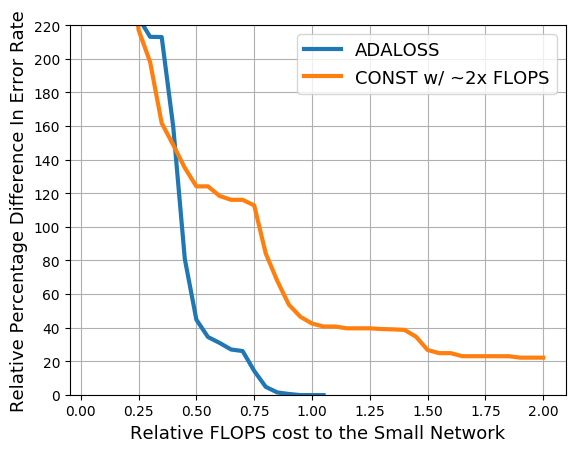
\includegraphics[width=0.32\linewidth, keepaspectratio ]{\ANNDIR/adaloss_vs_const_of_double_cost_cifar10.png}
        \label{fig:adaloss_vs_const_of_double_cost_cifar10}
    }
    ~
    \subfloat[Res\anns on CIFAR100]{
        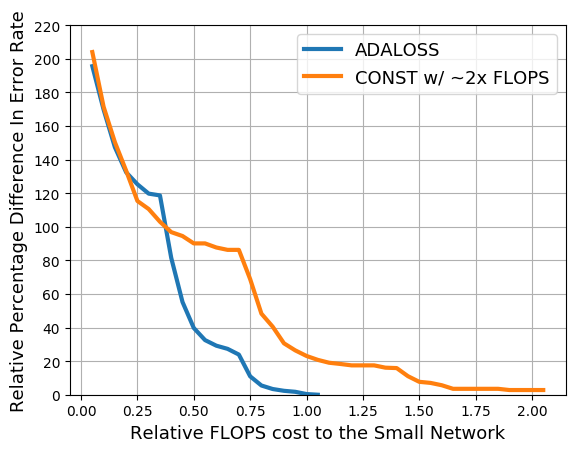
\includegraphics[width=0.32\linewidth, keepaspectratio ]{\ANNDIR/adaloss_vs_const_of_double_cost_cifar100.png}
        \label{fig:adaloss_vs_const_of_double_cost_cifar100}
    }
    ~
    \subfloat[Res\anns on SVHN]{
        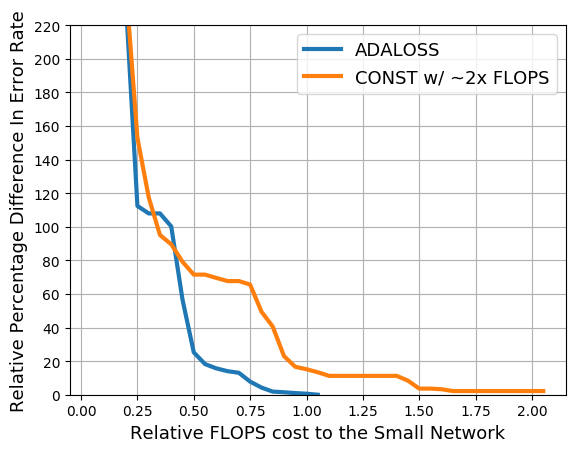
\includegraphics[width=0.32\linewidth, keepaspectratio ]{\ANNDIR/adaloss_vs_const_of_double_cost_svhn.png}
        \label{fig:adaloss_vs_const_of_double_cost_svhn}
    }
    
    \subfloat[Res\anns on ILSVRC]{
        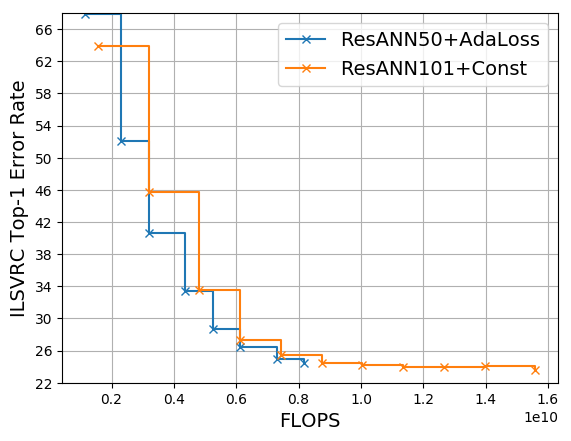
\includegraphics[width=0.32\linewidth, keepaspectratio]{\ANNDIR/ilsvrc_adaloss_vs_const_resnet.png}
        \label{fig:ilsvrc_adaloss_vs_const_of_double_cost}
    }
    ~
    \subfloat[MSDNet on ILSVRC]{
        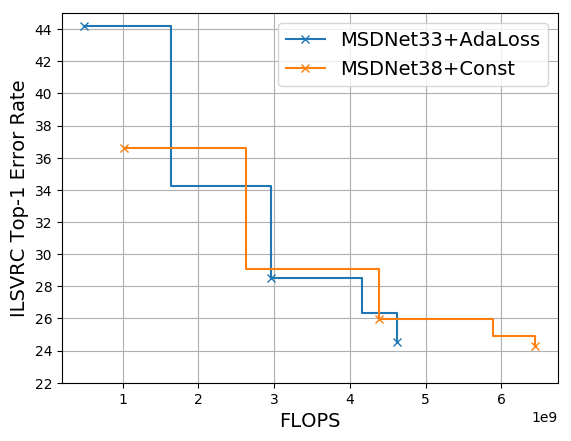
\includegraphics[width=0.32\linewidth, keepaspectratio]{\ANNDIR/ilsvrc_adaloss_vs_const_msdnet.png}
        \label{fig:ilsvrc_adaloss_vs_const_of_double_cost_msdnet}    
    }
    ~
    \subfloat[\anns comparison on ILSVRC]{
        \includegraphics[width=0.32\linewidth, keepaspectratio]{\ANNDIR/ilsvrc_compare_models.png}
        \label{fig:ilsvrc_compare_models}    
    }
    
    \caption{\textbf{(a-e)} Comparing small networks with \adaloss versus big ones using \const. With \adaloss, 
    the small networks achieve the same accuracy levels faster than large networks with \const. 
    \textbf{(f)} \anns performance are mostly decided by underlying models, but \adaloss is beneficial regardless models. }
    \label{fig:adaloss_vs_const_of_double_cost}
\end{figure*}
\textbf{\adaloss vs. \const on the same models.} Table~\ref{tab:compare_f} presents the average relative test error rate increase from OPT on 12  Res\anns on CIFAR10, CIFAR100 and SVHN\footnote{The 12 models are named by $(n,c)$ drawn from $\{ 7, 9, 13, 17, 25 \} \times \{ 16, 32 \}$ and $\{(9,64), (9,128)\}$, where $n$ represents the number of residual units in each of the three blocks of the network, and $c$ is the filter size of the first convolution.}. As training an OPT for each depth is too expensive, we instead report the average relative comparison at 1/4, 1/2, 3/4, and 1 of the total \ann costs. 
We observe that the \const scheme makes $15\sim 18\%$ more errors than the OPT, and the relative gap widens at later layers.  The \linear scheme also has about 13\% relative gap in later layers. In contrast, \adaloss enjoys small performance gaps in the later half of layers. 
On ILSVRC, we compare \adaloss against \const on Res\annnp50, Dense\annnp169, and MSDNet38, which have similar final errors and total computational costs (See Fig.~\ref{fig:ilsvrc_compare_models}). In Table~\ref{tab:compare_f_ilsvrc}, we observe the trade-offs between early and late accuracy on Res\annnp50 and MSDNet38. Furthermore, Dense\annnp169 performs \emph{uniformly} better with \adaloss than with \const. 
Since comparing the weight schemes requires evaluating \anns at multiple budget limits, and \adaloss and \const outperform each other at a significant fraction of depths on most of our experiments, we consider the two schemes \emph{incomparable on the same model}. 
%However, our next experiments will show late predictions to be vastly more important than the early ones.

\begin{figure*}[t]
    \centering
    \subfloat[EANNs on CIFAR100]{
        \includegraphics[width=0.32\linewidth, keepaspectratio]{\ANNDIR/cifar100_adaloss_eann_b2.png}
        \label{fig:eann_f}
    }
    ~
    \subfloat[EANN on ILSVRC]{
        \includegraphics[width=0.32\linewidth, keepaspectratio]{\ANNDIR/eann_comparisons.png}
        \label{fig:compare_ensemble}
    }
    ~
    \subfloat[AdaLoss Weights on three data-sets]{
    \includegraphics[width=0.32\linewidth, keepaspectratio]{\ANNDIR/adaloss_weights.png}
    \label{fig:adaloss_weights}
    }
    \caption{ \textbf{(a)} EANN performs better if the \anns use \adaloss instead of \const. 
    \textbf{(b)} EANN outperforms linear ensembles of DNNs on ILSVRC.
    \textbf{(c)} The learned adaptive weights of the same model on three data-sets.
    }
    %AANN-14 finishes at 33.50\% error,
\end{figure*}


\textbf{Small networks with \adaloss vs. large ones with \const.} 
Our previous comparison between \adaloss and \const on the same models is not fully conclusive, since each scheme can outperform the other at a significant portion of the total cost. To address this, we set the final error rate, model architecture type, and the filter size $c$ as constants, and vary the model depths so that \adaloss and \const reach the target final error rate. Then we compare the early predictions and the costs of models. 
On each of CIFAR10, 100 and SVHN, we compare six pairs of Res\anns, where the \const uses twice the computation as \adaloss\footnote{\adaloss takes $(n,c)$ from $\{7,9,13\} \times \{16, 32\}$, and \const takes $(n,c)$ from $\{13,17,25\} \times \{16, 32\}$.}. Fig.~\ref{fig:adaloss_vs_const_of_double_cost_cifar10},~\ref{fig:adaloss_vs_const_of_double_cost_cifar100}, and~\ref{fig:adaloss_vs_const_of_double_cost_svhn} show the averaged relative comparisons\footnote{The relative plots pivot at the final predictor from \adaloss, e.g., the location (0.5, 200) means having half the computation and 200\% extra relative errors than the final predictor from \adaloss}, and they show that the small \anns with \adaloss are better anytime predictors than the large ones with \const, because both models have the same final accuracy (on CIFAR10, the small ones are even better), and the small models reach the same error rates faster than the large ones. We have similar observations on ILSVRC using Res\anns and MSDNets in Fig.~\ref{fig:ilsvrc_adaloss_vs_const_of_double_cost} and Fig.~\ref{fig:ilsvrc_adaloss_vs_const_of_double_cost_msdnet}.
For instance, MSDNet~\cite{msdense} is the state-of-the-art anytime predictor. The published MSDNet38 uses \const, and has 24.3\% error rate using 6.6e9 total FLOPS in convolutions. By switching to \adaloss, we improve a much smaller MSDNet33 (details in the appendix), which costs 4.5e9 FLOPS, to reach 24.5\% final error. The two models also have similar early errors. 

\adaloss can reach the same accuracies with similar or smaller costs than \const, because in practice, a linear decrease in final error rate may often require an exponential increase in total computation, and \const degrades the final performances significantly (Table~\ref{tab:compare_f}). Since \adaloss requires much smaller models than \const to reach the same final errors, and with a fixed final error rate, \adaloss reaches each early error rate with less or similar cost, we conclude that \adaloss is the better scheme for anytime predictions. 

\textbf{Various base networks on ILSVRC.} We compare Res\anns, Dense\anns and MSDNets that have final error rate of near 24\% in Fig.~\ref{fig:ilsvrc_compare_models}, and observe that the anytime performance is mostly decided by the specific underlying model. MSDNets are more cost-effective than Dense\anns, which in turn are better than Res\anns. 
However, \adaloss is helpful regardless of underlying model. Both Res\annnp50 and Dense\annnp169 see improvements switching from \const to \adaloss, which is also shown in Table~\ref{tab:compare_f_ilsvrc}. 
Thanks to \adaloss, Dense\annnp169 achieves the same final error using similar FLOPS as the original published results of MSDNet38~\cite{msdense}. This suggests that~\cite{msdense} improve over Dense\anns by having better early predictions without sacrificing the final cost efficiency via impressive architecture insight. \adaloss brings a complementary improvement to MSDNets, as it enables smaller MSDNets to reach the final error rates of bigger MSDNets, while having similar or better early predictions. 



%%%%%%%%%%%%%%%%%% EANN %%%%%%%%%%%%%%%%%%%%%%%%

\subsection{EANN: Closing Early Performance Gaps by Delaying Final Predictions.}
\label{sec:eann_experiment}



\textbf{EANNs on CIFAR100.} In Fig.~\ref{fig:eann_f}, we assemble Res\anns to form EANNs\footnote{The Res\anns have $c=32$ and $n=7, 13, 25$, so that they form an EANN with an exponential base $b\approx 2$. 
By proposition~\ref{prop:eann}, the average cost inflation is $E[C]\approx 2.44$ for $b=2$, so that the EANN should 
compete against the OPT of $n=20$, using $2.44$ times of original costs.} on CIFAR100 and make three observations.
First, EANNs are better than the \ann in early computation, because the ensembles dedicate early predictions to small networks. Even though \const has the best early predictions as in Table~\ref{tab:compare_f}, it is still better to deploy small networks. 
Second, because the final prediction of each network is kept for a long period, \adaloss leads to significantly better EANNs than \const does, thanks to the superior final predictions from \adaloss. 
Finally, though EANNs delay computation of large networks, it actually appears closer to the OPT, because of accuracy saturation. Hence, EANNs should be considered when performance saturation is severe. 

\textbf{EANN on ILSVRC.}
\cite{msdense} and \cite{feedbacknet} use ensembles of networks of linearly growing sizes as baseline anytime predictors. However, in Fig.~\ref{fig:compare_ensemble}, an EANN using Res\anns of depths 26, 50 and 101 outperforms the linear ensembles of ResNets and DenseNets significantly on ILSVRC.
In particular, this drastically reduces the gap between ensembles and the state-of-the-art anytime predictor MSDNet~\cite{msdense}. 
Comparing Res\ann50 and the EANN, we note that the EANN achieves better early accuracy but delays final predictions. 
As the accuracy is not saturated by Res\ann26, the delay appears significant. Hence, EANNs may not be the best when the performance is not saturated or when the constant fraction of extra cost is critical. 


\subsection{Data-set Difficulty versus Adaptive Weights}
\label{sec:weight_vs_dataset}



In Fig.~\ref{fig:adaloss_weights}, we plot the final \adaloss weights of the same Res\ann model (25,32) on CIFAR10, CIFAR100, and SVHN to study the effects of the data-sets on the weights. We observe that from the easiest data-set, SVHN, to the hardest, CIFAR100, the weights are more concentrated on the final layers. This suggests that \adaloss can automatically decide that harder data-sets need more concentrated final weights to have near-optimal final performance, whereas on easy data-sets, more efforts are directed to early predictions. Hence, \adaloss weights may provide information for practitioners to design and choose models based on data-sets.

\section{Conclusion and Discussion}
This work devises simple adaptive weights, \adaloss, for training anytime predictions in DNNs. We provide multiple theoretical motivations for such weights, and show experimentally that adaptive weights enable small \anns to outperform large \anns with the commonly used non-adaptive constant weights. Future works on adaptive weights includes examining \adaloss for multi-task problems and investigating its ``first-order'' variants that normalize the losses by individual gradient norms to address unknown offsets of losses as well as the unknown scales. We also note that this work can be combined with orthogonal works in early-exit budgeted predictions~\cite{cascade_nn,adaptivenn} for saving average test computation. 


\section*{Acknowledgements} 
This work was conducted in part through collaborative participation in the Robotics Consortium sponsored by the U.S Army Research Laboratory under the Collaborative Technology Alliance Program, Cooperative Agreement W911NF-10-2-0016. 


%%%%%%%%%%%%%%%%%% BIB %%%%%%%%%%%%%%%%%%%%%%%%
%\bibliographystyle{aaai}
%{
%\bibliography{AAAI-HuH.2508}
%}

%%%%%%%%%%%%%%%%%% APPENDIX %%%%%%%%%%%%%%%%%%%%%%%%
%\appendix




\section{Sketch of Proof of Proposition~\ref{prop:eann}}
\begin{proof}
For each budget consumed $x$, we compute the cost $x'$ of the optimal that EANN is competitive against. The goal is then to analyze the ratio $C = \frac{x}{x'}$. 
The first ANN in EANN has depth 1. The optimal and the result of EANN are the same. Now assume EANN is on depth $z$ of ANN number $n+1$ for $n\geq 0$, which has depth $b^{n}$. \\
(Case 1) For $z \leq b^{n-1}$, EANN reuse the result from the end of ANN number $n$. 
The cost spent is $x = z + \sum _{i=0}^{n-1} b^i = z + \frac{b^n-1}{b-1}$. 
The optimal we compete has cost of the last ANN, which is $b^{n-1}$
The ratio satisfies:
\begin{align*} 
C &= x / x' = \frac{z}{b^{n-1}} + 1 + \frac{1}{b-1} - \frac{1}{b^{n-1}(b-1)} \\
&\leq 2 + \frac{1}{b-1} - \frac{1}{b^{n-1}(b-1)} 
< 2+ \frac{1}{b-1}. 
\end{align*}
Furthermore, since $C$ increases with $z$, 
\begin{align*}
&E_{z \sim Uniform(0, b^{n-1})}[C] \\
&\leq b^{1-n} \int _0 ^{b^{n-1}} 
    z b^{1-n}+ 1 + \frac{1}{b-1} \;dz \\
&= 1.5 + \frac{1}{b-1}.
\end{align*}
\\
(Case 2) For $b^{n-1} < z \leq b^n$, EANN outputs anytime results from ANN number $n+1$ at depth $z$. 
The cost is still $x = z +\frac{b^n-1}{b-1}$. The optimal competitor has cost $x' = z$.  Hence the ratio is 
\begin{align*}
C &= x/ x' = 1 + \frac{b^n-1}{z(b-1)} \\
&\leq 2 + \frac{1}{b-1} - \frac{1}{b^{n-1}(b-1)} 
< 2+ \frac{1}{b-1}.
\end{align*}
Furthermore, since $C$ decreases with $z$, 
\begin{align*}
&E_{z \sim Uniform(b^{n-1}, b^n)}[C] \\
& \leq 1 +  
   \frac{1}{b^n - b^{n-1}} \int _{b^{n-1}} ^{b^{n}} 
        \frac{b^n -1}{z(b-1)} \; dz  \\
&= 1 + \frac{(b - b^{1-n}) \ln{b}}{(b-1)^2} \\
&< 1 + \frac{b \ln{b}}{(b-1)^2} 
\end{align*}

Finally, since case 1 and case 2 happen with probability $\frac{1}{b}$ and $(1-\frac{1}{b})$, we have
\begin{align}
    \sup _B C &= 2+ \frac{1}{b-1} \\
\intertext{and}
    E_{B\sim Uniform(0, L)}[C] &\leq 1 - \frac{1}{2b} + \frac{1}{b-1} + \frac{\ln{b}}{b-1}.
\end{align}
We also note that with large $b$, $\sup _B C \rightarrow 2$ and $E[C] \rightarrow 1$ from above.
\end{proof}

If we form a sequence of regular networks that grow exponentially in depth instead of \ann, then the worst case happen right before a new prediction is produced. Hence the ratio between the consumed budget and the cost of the optimal that the current anytime prediction can compete, $C$, right before the number $n+1$ network is completed, is 
\[
    \frac{\sum _{i=1}^n b^i}{b^{n-1}} \xrightarrow[]{n\rightarrow \infty} \frac{b^2}{b-1} = 2 + (b-1) + \frac{1}{b-1} \geq 4. 
\]
Note that $(b-1) + \frac{1}{b-1} \geq 2$ and the inequality is tight at $b=2$. Hence we know $\sup _B {C}$ is at least 4. Furthermore, the expected value of $C$, assume $B$ is uniformly sampled such that the interruption happens on the $(n+1)^{th}$ network, is:
\begin{align*}
    E[C] &= \frac{1}{b^{n}} \int _0 ^{b^{n}} \frac{x + \frac{b^{n}-1}{b-1}}{b^{n-1}} \; dx \\ &\xrightarrow[]{n\rightarrow \infty} 1.5 + \frac{b-1}{2} + \frac{1}{b-1} \geq 1.5 + \sqrt{2} \approx 2.91.
\end{align*}
The inequality is tight at $b = 1 + \sqrt{2}$. With large $n$, since almost all budgets are consumed by the last few networks, we know the overall expectation $E_{B\sim Uniform(0, L)}[C]$ approaches $1.5 + \frac{b-1}{2} + \frac{1}{b-1}$, which is at least $1.5 + \sqrt{2}$.




\section{Implementation Details of \anns}
\label{sec:implementation_ann}


\textbf{CIFAR and SVHN Res\anns.} For CIFAR10, CIFAR100~\cite{cifar}, and SVHN~\cite{svhn}, Res\ann follow \cite{resnet} to have three blocks, each of which has $n$ residual units. Each of such basic residual units consists of two 3x3 convolutions, which are interleaved by BN-ReLU. A pre-activation (BN-ReLU) is applied to the input of the residual units. The result of the second 3x3 conv and the initial input are added together as the output of the unit. The auxiliary predictors each applies a BN-ReLU and a global average pooling on its input feature map, and applies a linear prediction. The auxiliary loss is the cross-entropy loss, treating the linear prediction results as logits. For each $(n,c)$ pair such that $n < 25$, we set the anytime prediction period $s$ to be 1, i.e., every residual block leads to an auxiliary prediction. We set the prediction period $s=3$ for $n=25$. 


\textbf{Res\anns on ILSVRC.} Residual blocks for ILSVRC are bottleneck blocks, which consists of a chain of 1x1 conv, 3x3 conv and 1x1 conv. These convolutions are interleaved by BN-ReLU, and pre-activation BN-ReLU is also applied. Again, the output of the unit is the sum of the input feature map and the result of the final conv. 
Res\annnp50 and 101 are augmented from ResNet50 and 101~\cite{resnet}, where we add BN-ReLU, global pooling and linear prediction to every two bottleneck residual units for ResNet50, and every three for ResNet101. 
We create Res\annnp26 for creating EANN on ILSVRC, and Res\annnp26 has four blocks, each of which has two bottleneck residual units. The prediction period is every two units, using the same linear predictors. 


\textbf{Dense\anns on ILSVRC.} We augment DenseNet169~\cite{densenet} to create Dense\ann169. 
DenseNet169 has 82 dense layers, each of which has a 1x1 conv that project concatenation of previous features to $4k$ channels, where $k$ is the growth rate~\cite{densenet}, followed by a 3x3 conv to generate $k$ channels of features for the dense layer. The two convs are interleaved by BN-ReLU, and a pre-activation BN-ReLU is used for each layer. The 82 layers are organized into four blocks of size 6, 12, 32 and 32. Between each neighboring blocks, a 1x1 conv followed by BN-ReLU-2x2-average-pooling is applied to shrink the existing feature maps by half in the hight, width, and channel dimensions. We add linear anytime predictions every 14 dense layers, starting from layer 12 (1-based indexing). The original DenseNet paper~\cite{densenet} mentioned that they use drop-out with keep rate 0.9 after each conv in CIFAR and SVHN, but we found drop-out to be detrimental to performance on ILSVRC.


\textbf{MSDNet on ILSVRC.} MSDNet38 is described in the appendix of~\cite{msdense}. We set the four blocks to have 10, 9, 10 and 9 layers, and drop the feature maps of the finest resolution after each block as suggest in the original paper. 
We successfully reproduced the published results to 24.3\% error rate on ILSVRC using our Tensorflow implementation. We used the original published results for MSDNet38+\const in the main text. We use MSDNet33, which has four blocks of 8, 8, 8 and 9 layers, for the small network that uses \adaloss. We predict using MSDNet33 every seven layers, starting at the fifth layer (1-based indexing). 



\section{Additional Details of \adaloss}

\label{sec:implementation_adaloss}


\subsection{Weight Regularization} 
In practice, some expected loss $\ell_i$ could be much larger than the other losses, so that \adaloss may assign such $\ell_i$ too small a weight for it to receive enough optimization to recover. To prevent this, we mix the uniform constant weight with \adaloss as a form of regularization as follows in Eq.~\ref{eq:geometric_arithmetic_mean}. Such mixture prevents the weight of $\ell_i$ from being too close to zero. 
\begin{align}
    \min _{\theta} \sum _{i=1}^L \big( \alpha (1 - \gamma) \ln \ell _i (\theta) + \gamma  \ell_i (\theta) \big),
    \label{eq:geometric_arithmetic_mean}
\end{align}
where $\alpha >0$ and $\gamma >0$ are hyper parameters. In practice, since DNNs often have elaborate learning rate schedules that assume $B_L=1$, we choose $\alpha  = \min_i \hat{\ell}_i(\theta)$ at each iteration to scale the max weight to 1. We choose $\gamma = 0.05$ from validation sets on CIFAR10 and CIFAR100 from the set $\{0, 0.05, 0.15\}$.

\subsection{Ablation Study of \adaloss parameters on CIFAR} 


\begin{table}[t]
    \centering
    \begin{tabular}{c|cccc|c}
\hline
$\gamma$ & 1/4 & 1/2 & 3/4 & 1  & sum\\
\hline
0.0
	&  0.00 &  0.00 &  0.00 &  0.00  & 0.00\\
0.05
	& -20.08 & -2.15 &  2.22 &  2.43 & -17.59 \\
0.15
	& -23.88 & -0.20 &  5.18 &  5.17 & -13.72\\
\hline
    \end{tabular}
    \caption{Relative percentage increase in error rate by switching from $\gamma=0$. (lower is better.) A small amount of $\gamma = 0.5$ drastically improves early predictions without increasing late error rate much.}
    \label{tab:adaloss_gamma}
\end{table}


\begin{table}[t]
    \centering
    \begin{tabular}{c|cccc}
\hline
EMA $m$ & 1/4 & 1/2 & 3/4 & 1 \\
\hline
0.9
	&  0.00 &  0.00 &  0.00 &  0.00 \\
0.99
	& -0.29 &  0.25 &  0.05 &  0.15 \\
\hline
    \end{tabular}
    \caption{Relative percentage increase in error rate by switching from $m=0.9$.  (lower is better.) The two options essentially result in the same error rates.}
    \label{tab:adaloss_momentum}
\end{table}

\begin{table}[h!]
    \centering
    \begin{tabular}{c|cccc}
\hline
Update period $e$ & 1/4 & 1/2 & 3/4 & 1 \\
\hline
1
	&  0.00 &  0.00 &  0.00 &  0.00 \\
100
	&  0.71 &  0.23 &  0.24 &  0.45 \\
\hline
    \end{tabular}
    \caption{Relative percentage increase in error rate by switching from $e=0$.  (lower is better.) The options are essentially the same on CIFAR10 and CIFAR100. }
    \label{tab:adaloss_update_per}
\end{table}

We conduct ablation studies for the parameters of \adaloss: (1) $\gamma$ in Eq.~\ref{eq:geometric_arithmetic_mean}, which is the mixture weight of the uniform static weighting, (2) the exponential moving average (EMA) momentum, $m$, for updating the expected loss $\hat{\ell}_i$ at each stochastic gradient descent (SGD) step, and (3) the number of SGD steps $e$ to wait between updating \adaloss weights $B_i$ using the learned $\hat{\ell}_i$. We choose $\gamma \in \{0, 0.05, 0.15 \}$, $m \in \{0.9, 0.99\}$, and $e \in \{1, 100\}$, and evaluate them on CIFAR10 and CIFAR100 ResANNs whose $n \in \{9,17,25\}$ and $c=32$. Over the 72 experiments, we found the effects of $m$, and $e$ are almost negligible, as they generate $<0.5\%$ of relative difference in error rates on average, which translates to $0.1\%$ absolute error difference on CIFAR100. These comparisons are in Table~\ref{tab:adaloss_momentum} and Table~\ref{tab:adaloss_update_per}. In the experiment sections, we choose $m = 0.9$ and $e=1$.

However,  $\gamma$ does affect the performance significantly, as show in Table~\ref{tab:adaloss_gamma}. $\gamma=0$ means pure \adaloss and $\gamma=1$ means \const. We observe that with $\gamma=0.05$, the small amount of uniform static weight reduces the error rate at 1/4 of the total cost by 20\% relatively, but at the cost of minor 2.5\% relative increase in late predictions. Increasing $\gamma$ further to $0.15$ has only marginal benefits to early predictions, but has the same negative impact to late accuracy. This suggests that while a small $\gamma$ helps, we should only use a small amount. Throughout the experiment sections in the main text, we choose $\gamma = 0.05$.



\chapter{Neural Network Search}

%\begin{abstract}
%When developing predictors for machine learning applications, practitioners often want to have simple and working predictors early and continue to improve them with available computational resources. 
%In this work, we propose a neural architecture search (NAS) algorithm that iteratively augments existing networks by adding shortcut connections and layers. At each iteration, we greedily select among the most cost-efficient models a parent model, and insert into it a number of candidate layers.  To learn which combination of additional layers to keep,  we simultaneously train their parameters and select the most promising candidates via feature selection techniques. The selected candidates are then jointly trained with the parent model.  Within 15 GPU-days, the proposed network growth NAS algorithm (\Petridish) can already find a model on CIFAR-10 that achieves 2.79\% error rate using 2.8M parameters.  We also transfer the model to ILSVRC2012, and it achieves 25.4\% top-1 error rate using 6.2M parameters and 810M multiply-adds. 
%Furthermore, unlike recent studies of NAS that almost exclusively focus on the small search space of repeatable network modules (cells), this work also shows that a direct search among the more general networks (macro) can also find cost-effective models when macro search is allowed to start with the same initial models as cell search does. 
%\end{abstract}

\section{Introduction}
\label{sec:nas_introduction}

Deep neural networks have achieved state-of-the-art performance on many large scale supervised learning tasks across many domains like computer vision, natural language processing and audio and speech-related tasks. But most gains have come from manually designed architectures which have inspired further improvements via careful experimentation coupled with significant experience and intuition of a skilled practitioner. Such skilled practitioners usually have significant domain knowledge of the task at hand that allows them to make rapid progress. But the fact remains that the task of designing a deep network architecture from scratch remains mostly a game of trial and error. As a consequence there has been significant effort in the community to address this issue via attempts to design algorithms that automatically find good architectures and informally referred to as AutoDNN and/or Neural Architecture Search (NAS) \cite{nas}. 

NAS literature can be broadly categorized along three main dimensions: 1. search space 2. search procedure and 3. performance estimation strategy during the search procedure. The search space can be broadly further divided to methods that search either 1. a more general space of architectures often termed as macro-search or 2. a more constrained search space called micro or cell-search. In cell-search a good outer skeleton is often assumed. For example in image classification datasets it is common to often assume either ResNet~\citep{resnet} or DenseNet~\cite{densenet} style outer skeletons. The search can then be restricted to finding cells that fill in the slots in the outer skeleton so that the overall architecture has good performance. Cell-search is much more popular due to a number of reasons: 1. One can leverage domain knowledge of experts who have painstakingly come up with good architectures and focus the search to a smaller space. 2. Transfer to larger datasets where more capacity is often needed can be obtained by trivially stacking many cells to create larger networks. The very aspects that make cell-search attractive also prevent it from providing a truly general solution: when good outer skeletons are not available for novel domains/datasets or there is reason to believe that significant performance is left on the table, cell-search cannot be applied. By restricting the search space it is quite possible that significant performance is left on the table. On large datasets in production environments this feature is especially important. Macro-search in principle doesn't suffer from any of the above limitations but suffers from searching a much more general and larger architecture space. 

In this work we propose a method for growing networks from small to large where we opportunistically add layers inspired by the ``cascade correlation'' work of \cite{cascadecorr}. We term our approach \Petridish. \Petridish can be used with both macro and cell-search spaces. Importantly \Petridish achieves better performance on macro search spaces than any other NAS algorithm which considers macro search results. Furthermore the final results achieved by \Petridish macro are comparable to those of the current best cell-search methods including that of \Petridish cell-search methods.

\begin{itemize}
\item We propose an approach to increase complexity of neural networks during training iteratively. We alternate between two phases. The first expands the model with potential shortcut connections and train them jointly. The second phase trim the previous potential connections using feature selection and continue training the model. 
\item The proposed approach can be applied to both improve a small repeatable pattern, called cell, and improve the macro network architecture directly, unlike most popular approaches that only focus on cells. This opens up neural architecture search to fields where no domain knowledge of the macro structure exists. 
\item On cell-search, the proposed method finds a model that achieves 2.61\% error rate on CIFAR10 using 2.9M parameters within 5 GPU-days. 
The model achieves 26.0\% error rate on ILSVRC2012 using 4.8M parameters and 598M multi-adds.
\item On macro-search, the proposed method finds a model that achieves 2.83\% error rate on CIFAR10 using 2.2M parameters within 5 GPU-days. 
%The model achieves \% error rate on ILSVRC2012 using M parameters and M multi-adds.
\item The proposed approach can warm start from existing networks, leveraging previous training results. Furthermore, it directly expands models on the lower convex hull of error rate vs. flops and is hence able to naturally produce a gallery of cost-effective models which is critical for production serving needs. 
\end{itemize}


\section{Related Works}
\label{sec:nas_background}
%\begin{itemize}
%    \item Cascade-correlation
%    \item NAS. (RL. EA. Gradient based.) 
%    \item (Micro. Macro.) 
%    \item Multi objective NAS; Pareto Front Nas 
%    \item Evaluation with few epochs vs many epochs
%    \item Incremental training, AdaNet, Boosted ResNet, Net morphism
%    \item Test~\cite{nas, NASCell, Hsu2018MONASMN, Elsken2018NeuralAS, Real2018RegularizedEF, Liu2018DARTSDA, Kandasamy2018BNAS, Pham2018EfficientNA, Liu2017ProgressiveNA}
%\end{itemize}

One of the earliest architecture search work was by \cite{cascadecorr} termed the ``Cascade-Correlation Learning Architecture'' (C2) which has inspired \Petridish. In C2 the search begins with a minimal network which is trained by any routine training algorithm like backpropagation with stochastic gradient descent. Once training error saturates C2 considers adding a candidate hidden neuron. The candidate hidden neuron before insertion to the network is connected to the input neurons and all currently existing hidden neurons. The weights of the incoming connections to this shadow neuron are optimized such that the correlation between the activations of this shadow neuron and the error at the output neurons is maximized. Then the shadow neuron is inserted into the network and its incoming weights are frozen. Its outgoing weights are then trained in the usual way. There are various similarities between C2 and \Petridish which we discuss in Sec.~\ref{sec:soft_vs_hard}.
C2 is also one of the first works that studies the idea of gradually expanding neural networks during training. This idea was studied recently by~\citep{adanet, boostedresnet} through the view of boosting small networks in the context of modern networks. 

The work of \citep{nas,NASCell} renewed interest in NAS in recent times. Their method uses a recursive neural network (RNN) as a controller network which is used to sample architectures. Each of these architectures are trained on separate machines and their resulting accuracies are used to update the parameters of the controller network via policy gradients~\citep{policygradient}. The majority of the time is spent in training each of the sampled architectures in parallel on independent machines. The resulting search times are generally on the order of thousands of GPU hours (See Table~\ref{tab:cifar10_search}). \cite{Pham2018EfficientNA} introduced a much more efficient version of this algorithm termed as Efficient Neural Architecture Search (ENAS) where the controller samples network architectures from a large super-graph of all possible architectures but trains them all jointly where the weights of edges which are common amongst the sampled architectures are shared across all of them at training time. This leads to orders of magnitude improvement in search times but still has the restriction that a super-graph to sample from must be constructed apriori.
\cite{Liu2017ProgressiveNA} proposed a method which instead of using policy gradients as in \cite{NASCell}, trains predictors on the results of training a batch of architectures to predict top-K architectures which are likely to do well in subsequent rounds in a progressive manner and hence termed as Progressive Neural Architecture Search (PNAS). 
\cite{Liu2018DARTSDA} proposed a novel method based on bilevel optimization~\citep{bilevel_opt} termed as Differentiable Architecture Search (DARTS) which relaxes the originally discrete optimization problem to a continuous one and maintains two sets of continuous parameters: 1. The (architecture) parameters over the layer types and 2. The regular parameters of the network itself for each layer type. This is optimized in an alternating fashion where first the architecture parameters are trained alternated by the parameters of the layers of each type. Discrete architectures are then backed out by just selecting the architecture parameters which have the maximum value and discarding others. DARTS achieves impressive results on cell-search space with short search times.
\cite{Elsken2018EfficientMN, CaiPathLevel} proposed an alternative insight to speed up search by incrementally evolving models from existing cost-effective models. In particular,~\cite{Elsken2018EfficientMN} explore expanding the Pareto-frontier, a set of points that do not have strict superior points, of the parameter-versus-accuracy plot to find parameter-efficient models. We refer the reader to the excellent survey article by \cite{Elsken2018NeuralAS} for more details on this rapidly evolving field. 


\section{Neural Architecture Search as Optimization}

Given a data sample $x$ with label $y$, a neural network architecture $\alpha$ with parameters $w$ produces 
a prediction $\hat{y}(x ; \alpha, w)$ and suffers a prediction loss $\ell(\hat{y}(x ; \alpha, w), y)$.
The empirical training loss is then 
\begin{align}
\mathcal{L}(\alpha, w) = \mathbb{E} _{x, y \sim \mathcal{D}} [ \ell(\hat{y}(x ; \alpha, w), y) ] ,
\end{align}
where $\mathcal{D}$ is the empirical training data. 
Then the problem of neural architectures search can be formulated as a bi-level optimization~\citep{bilevel_opt}
of both the network architecture $\alpha$ and the model parameters $w$ under the expected training loss $\mathcal{L}$ 
as follows.
\begin{align}
\min _{\alpha} \mathcal{L} (\alpha, w(\alpha)),
\quad
s.t. \quad w(\alpha) = \argmin _w \mathcal{L} (\alpha, w) 
\quad and \quad c(\alpha) \leq K,
\label{eq:bilevel_nas}
\end{align}
where $c(\alpha)$ represents the test-time computational cost of the architecture, and $K$ is some constant. 

We formalize $\alpha$ as a set of discrete decisions on which operations to include in an architecture.
Let $x_1, x_2,...,$ be intermediate layers, and $x_0 = x$ is the input. Each layer $x_i$ is a function
of the previous layers, i.e., $x_{i} = f_i ( x_0, x_1,..., x_{i-1})$ for some function $f_i$, 
though it is not necessary for $x_i$ to directly use each of the previous layers.
Each shortcut connection is defined by a triple $(x_{j}, x_{i}, op)$, 
where $x_j$ and $x_i$ ($j < i$) represent the input and output layers, and $op$ is a unary operation such 
as conv 3x3 and max pooling 3x3. Such a shortcut results in a tensor $op(x_{j})$ that can be used directly by 
$x_i$. Shortcuts to $x_i$ are combined by a merge operation 
at $x_i$, such as averaging, summation, or concatenation in order to form $x_i$.
In this work, we set the merge operations with ablation studies. 
Instead, we focus on the choice of the shortcut connections, i.e., each $\alpha$ is 
an unordered collection of $(x_j, x_i, op)$. 

                   
                   
                   
                                                                         
\subsection{Connection to Feature Selection}

Before delving into a proposed approach, we first draw an interesting connection of Eq.~\ref{eq:bilevel_nas}
to a well studied problem, feature selection for linear predictions, whose optimization formulation follows.
\begin{align}
&\min _{\alpha} \frac{1}{2n} \Vert Y - X_{\alpha} w(\alpha) \Vert ^2 + \frac{\lambda}{2} \Vert w \Vert ^2 \\
&s.t. \quad w(\alpha) = (\frac{1}{n}X_{\alpha}^TX_{\alpha} + \lambda I)^{-1} \frac{1}{n} X_{\alpha}Y 
\quad and \quad c(\alpha) \leq K,
\label{eq:bilevel_gomp}
\end{align}
where $X \in \mathcal{R}^{n \times d}$ is the feature matrix of the $n$ samples of $d$-dimensional features,
$Y \in \mathcal{R}^n$ is the regression targets, and $X_{\alpha}$ selects the features included in $\alpha$.
We note that Eq.~\ref{eq:bilevel_nas} generalizes Eq.~\ref{eq:bilevel_gomp}, since $w(\alpha)$ solves for the 
optimal coefficient given the selected features.

This observation permits us to translate between existing NAS algorithm to the feature selection problem. 
In particular,~\citep{nas,Real2017EvoNet} apply reinforcement learning and evolutionary algorithm to 
guide the trials of architecture $\alpha$, and train the potential architectures independently. 
Such methods, when applied to feature selection, are equivalent to exploring all subset of features 
using reinforcement learning or evolutionary algorithms. As a result, it is understandable that
they search for thousands of GPU-days. 

In contrast, the more recent works~\citep{Pham2018EfficientNA,Liu2018DARTSDA} train all possible
networks at the same time by training the super-graph that contains all possible shortcut connections.
Then they train at the same time a selection procedure to select the most promising 
sub-graph from this super-graph. Such procedures draw parallel to backward elimination 
and sparse optimization for feature selection, 
where the irrelevant features are iteratively removed or down-weighted. 

Besides exhaustive search, sparse optimization and backward elimination, there is another popular branch of approaches 
for feature selection, forward selection, where feature are iteratively selected, or their coefficients are gradually increased. 
Unfortunately, common algorithms such as 
Forward Regression (FR) and its approximation Orthogonal Matching Pursuit (OMP),
cannot 
directly be applied to the NAS problem, because both methods require computing 
$w(\alpha)$ at each architecture, and such computation takes a GPU-day on its own. Instead, we have
to consider methods that approximate $w(\alpha)$ and $\alpha$ at the same time. Fortunately,
one such forward algorithm for feature selection is Least-angle regression (LARS)~\citep{lars}. 

In LARS, we compute the correlation between the residual of linear prediction and
each feature, and find the feature with the largest absolute correlation. Then we update the 
coefficient of this feature until its absolute correlation is no longer the largest.
One practical approximation of LARS is to iteratively update the coefficients of the most 
correlated feature with small steps, so that we avoid computing the line search analytically. 
Under this modification, LARS can be viewed as gradient boosting with small step sizes.
In Eq.~\ref{eq:bilevel_nas}, the gradient of the empirical loss with respect to the prediction is 
\begin{align}
\nabla _{\hat{y}} \mathcal{L} (\alpha, w) = \mathbb{E} _{x, y \sim \mathcal{D}} [ \nabla _{\hat{y}} \ell(\hat{y}(x ; \alpha, w), y) ].
\label{eq:nas_func_g_y}
\end{align}
Under linear prediction, this gradient becomes the residual up to a constant, 
$
\nabla _{\hat{y}} \mathcal{L} (\alpha, w) = \frac{1}{n}(X_{\alpha}w(\alpha) - Y).
$
Under linear predictions, features can be viewed as weak learners. 
Hence, the correlations between the features and the residual are
the correlations between the weak learners and the functional gradient with respect to predictions.
The selected weak learner is then the one that can match the gradient the most, i.e., 
LARS follows gradient boosting to select weak learners.






\section{A NAS Approach from Gradient Boosting}


This section first briefly reviews gradient boosting, and 
then describes the proposed method as an iterative optimization of Eq.~\ref{eq:bilevel_nas}. 
Then we delve into implementation details, including the search space and  
how to match the gradient efficiently.


\subsection{Gradient Boosting}
\label{sec:gb_review_nas}
Let $\mathcal{H}$ be a space of weak learners. 
Gradient boosting matches weak learners $h \in \mathcal{H}$ to 
the functional gradient of the loss $\mathcal{L}$ with respect to the prediction $\hat{y}$, 
i.e., $\nabla _{\hat{y}} \mathcal{L}$ in Eq.~\ref{eq:nas_func_g_y}.
The weak learner that matches the negative gradient the best, $h^*$, is added to the ensemble of learners, i.e.,
\begin{align}
h^* = \argmin _{h \in \mathcal{H}} \langle \nabla _{\hat{y}} \mathcal{L}, h \rangle.
\end{align}
Then the predictor is updated to become $\hat{y} \leftarrow \hat{y} + \eta h^*$, where $\eta$ is the learning rate.

\subsection{Gradient-Boosting-Inspired NAS}
\label{sec:gb_nas}
Following gradient boosting strictly would limit the model growth to be only at the prediction of the network, $\hat{y}$. 
Instead, this work seeks to expand the expressiveness of the network at intermediate layers, $x_1, x_2,...,$, jointly.
Inspired by gradient boosting, we considering adding a weak learner $h_i \in \mathcal{H}_i$ at each $x_i$, where 
$\mathcal{H}_i$ is the space of weak learners for layer $x_i$ and we will specify it shortly. 
$h_i$ helps reduce the gradient of the loss $\mathcal{L}$ with respect to $x_i$, $\nabla _{x_i} \mathcal{L}  = \mathbb{E} _{x, y \sim \mathcal{D}} [ \nabla _{x_{i}} \ell(\hat{y}(x ; \alpha, w), y) ]$.
i.e., we choose $h_i$ with 
\begin{align}
h_i = \argmin _{h \in \mathcal{H}_i} \langle h, 
\nabla _{x_i} \mathcal{L} (\alpha, w) \rangle = 
\argmin _{h\in \mathcal{H}_i} \langle h, \mathbb{E} _{x, y \sim \mathcal{D}} [ \nabla _{x_{i}} \ell(\hat{y}(x ; \alpha, w), y) ] \rangle.
\label{eq:hallu_objective}
\end{align}
Then we expand the model by adding a small step $\eta$ in the direction of $h_i$ to $x_i$, i.e., we replace each $x_i$ with $x_i + \eta h_i$ in the original network.
Throughout this work, we set the merge operation at the expansion location $x_i$ to be summation for simplicity.

Sec.~\ref{sec:search_space} details the search space such as choice of $x_i$ and $\mathcal{H}_i$. 
Sec.~\ref{sec:candidate_init_and_select} details how to approximate Eq.~\ref{eq:hallu_objective} efficiently via 
a joint optimization of weak learners, warm-starting from some existing models.
Sec.~\ref{sec:candidate_finalize} details how we finalize the selected weak learner $h_i$ for layer $x_i$.
Sec.~\ref{sec:parent_choice} details how to choose which model to apply the network growth.



\subsection{Search Space}
\label{sec:search_space}

\textbf{Cell-search vs. Macro-search.}
In this work, we consider both cell-search, 
a popular NAS search space where networks are described as repeats of some connection patterns~\citep{NASCell,Real2018RegularizedEF,Pham2018EfficientNA,Liu2018DARTSDA}, 
and macro-search, a more general NAS where no repeatable patterns are required. 
For a fair comparison of the two, we set the only difference between the two to be whether the connection pattern is repeated. Specifically, both start with the same initial seed model, which is a network build with simple cells.
Both search add weak learners at the same locations and at the same rate: one weak learner is always added to the end output of each cell per growth iteration, except that cell-search adds the same connection pattern to each cell, and macro-search allows different patterns. 
The space of the weak learners, which we detail next, is the same for both search. 



\textbf{Weak Learner Space $\mathcal{H}$.}
Given an intermediate layer $x_{k}$ to expand at, its associated weak learner space $\mathcal{H}_{k}$ is defined by four terms: the possible inputs, the
possible unary operations on the inputs, a merge operation to combine the results, and the maximum number of inputs. 
Following~\citep{NASCell,Real2018RegularizedEF,Liu2018DARTSDA}, we limit weak learners to only take input from layers within the same cell or from the output layers of the previous 
two cells. Let the collection of eligible input layers be $\text{In}(x_{k})$. 
The eligible unary operations are dependent on data-set. Following~\citep{Liu2018DARTSDA}, seven operations are eligible for vision tasks, and they are
separable conv 3x3 and 5x5, dilated conv 3x3 and 5x5, max and average pooling 3x3, and identity. Following~\citep{NASCell,Real2018RegularizedEF}, the separable conv is 
repeated twice. The outputs of the unary operations are of the same shape 
as the output location $x_k$. 
Let the collection of eligible unary operations be $\text{Op}$.
Since we restrict the merge operation between weak learners and $x_{k}$ to be summation, we found through ablation study in Sec.~\ref{sec:sum_vs_cat_proj} that
it is substantially better to merge the operations in the weak learners via a concatenation followed by a conv 1x1 to reduce the channel size. 
The maximum number of inputs is also data-set dependent, and for vision tasks, we set it to be $I_{max} = 3$, which is an empirical result from~\citep{darts_gumbel}.
Then the weak learner space $\mathcal{H}_{k}$ for a layer $x_{k}$ is formally 
\begin{align}
\mathcal{H}_{k} = \{ \text{cat\_proj}( op_1(z_1), ..., op_{I_{max}}(z_{I_{max}})) : z_1, ..., z_t \in \text{In}(x_{k}), op_1, ..., op_{I_{max}} \in \text{Op}  \}.
\end{align}



\textbf{Additional Search Space Details.}
For the vision tasks, the initial model for both macro and cell-search is a modified ResNet~\citep{resnet}, where we replace each 3x3 convolution with a 3x3 separable convolution. This is one of the simplest cell within the search space of existing literature~\citep{NASCell,Pham2018EfficientNA,Liu2018DARTSDA}.  Following ~\citep{NASCell}, we have six regular cells for each of the three resolutions of feature maps during training of the final found architectures, 
but have three regular cell per resolution during search. Similarly, we have an initial channel size of $F=32$ during final training and $F=16$ during search. 
A transition cell is in between each neighboring resolutions, and it also starts as a modified residual unit. 
When we transfer the model to larger data-sets that require more than three resolutions, we use transition cells to first down-sample the image height and width to be no greater than 32 and then apply the found model. In macro-search, where no transition cells are specifically learned, we again use the the modified ResNet cells for initial transition in the transferred model.


\subsection{Joint Weak Learning}
\label{sec:candidate_init_and_select}

\begin{algorithm}[t]
\begin{algorithmic}[1]
\STATE \textbf{Input}: 
(1) $L_x$, the list of layers in the current model (macro-search) or current cell (cell-search) in topological order;
(2) $\texttt{is\_out}(x)$, whether we can expand at $x$;
(3) $\texttt{is\_frozen}$, whether to freeze the influence from candidates to the parent;
(4) $\lambda$, hyper parameter for selection shortcut connections. 
\STATE \textbf{Output}: (1) $L'_x$, the modified $L_x$ with weak learners $x_c$; 
(2) $L_c$, the list of $x_c$ created;
(3) $\ell_{extra}$, the additional training loss.

\STATE $L'_x \leftarrow L_x$
\STATE $L_c \leftarrow \text{empty list}$
\STATE $\ell_{extra} \leftarrow 0$ 
\FOR{$x_k$ in enumerate($L_x$)}
    \IF { not \texttt{is\_out}($x_{k}$)}
        \STATE continue
    \ENDIF
    \STATE Compute the eligible inputs $\text{In}(x_{k})$, and index them as $z_1,...,z_I$.

    %\STATE Initialize $\alpha_{i,j}$ randomly from Gaussian. 
    %\STATE Initialize parameters in $op_j(x_{in,i})$. 
    \IF { $\texttt{is\_frozen}$ }
        \STATE $x_c \leftarrow \sum _{i=1}^I \sum _{j=1}^J  \alpha^k_{i,j}op_j(\stopgradient (z_i))$.
        \label{algline:add_sg}
    \ELSE
        \STATE $x_c \leftarrow \sum _{i=1}^I \sum _{j=1}^J  \alpha^k_{i,j}op_j(z_i)$.
    \ENDIF
\STATE Insert the layer $x_c$ right before $x_{k}$ in $L'_x$.
\STATE $\ell_{extra} \leftarrow \ell_{extra} + \lambda \sum _{i=1}^I \sum _{j=1}^J |\alpha^k_{i,j}|$.
\STATE Append $x_c$ to $L_c$.
\IF { $\texttt{is\_frozen}$ }
    \STATE Modify $x_{k}$ in $L'_x$ so that $x_{k} \leftarrow x_{k} + \stopforward (x_c)$.
    \label{algline:add_sf}
\ELSE
    \STATE Modify $x_{k}$ in $L'_x$ so that $x_{k} \leftarrow x_{k} + x_c$.
\ENDIF
\ENDFOR
\end{algorithmic}
\caption{Initialize Candidates}
\label{alg:candidate_init}
\end{algorithm}

\begin{algorithm}[t]
\begin{algorithmic}[1]
\STATE \textbf{Inputs}: (1) $L'_x$, the list of layers of the model in topological order;
(2) $L_c$, list of selection modules in $L'_x$;
(3) $\alpha^k_{i,j}$, the learned weights of the each $x_c$. 
\STATE \textbf{Output}: A modified $L'_x$ with selected operations.
\FOR{$x_c$ in $L_c$}
    \STATE Let $A = \{\alpha^{k}_{i,j}: i = 1,..., I, j = 1,..., J\}$  be the weights of operations in $x_c$.
    \STATE Sort $\{ |a| : a \in A \}$, and let the operations associated with the largest $I_{max}$ value be $op_1, ..., op_{I_{max}}$.
    \STATE Replace $x_c$ with $\text{proj}(\text{concat}(op_1, ..., op_{I_{max}}))$ in $L'_x$.
\ENDFOR
\STATE Replace all $\stopforward (\cdot)$ and $\stopgradient (\cdot)$ with identity in $L'_x$.
\end{algorithmic}
\caption{Select and Finalize Candidates}
\label{alg:candidate_select}
\end{algorithm}


Given an intermediate layer $x_{k}$ to expand at, we have $I = |\text{In}(x_{k})|$ possible input layers and $J = |\text{Op}|$ possible operations.
Hence, there are $\binom{IJ}{I_{max}}$ possible weak learners
in the space $\mathcal{H}_{k}$, and it is computationally expensive to train each weak learner individually. 
Inspired by the parameter sharing works in NAS~\citep{Pham2018EfficientNA,Liu2018DARTSDA} and model compression in neural networks~\citep{huang2017condensenet},
we propose to jointly train the weak learners in the union of them, 
and at the same time learn to select the shortcut connections. 


Algorithm~\ref{alg:candidate_init} describes the proposed approach to train the weak learners. 
For now, let us assume the boolean variable
$\texttt{is\_frozen}$ is true in the algorithm. This means that the weak learning does not from affecting the parameter of the current model. 
Fig.~\ref{fig:x_c_select_sf_sg} illustrates the weak learning modification to the current network. 

\begin{figure}[ht]
\centering
\subfloat[]{
    \includegraphics[width=0.44\textwidth, keepaspectratio]{\NASDIR/img/x_c_select.png}
    \label{fig:x_c_select}}
    ~
\subfloat[]{
    \includegraphics[width=0.44\textwidth, keepaspectratio]{\NASDIR/img/x_c_select_sf_sg.png}
    \label{fig:x_c_select_sf_sg}}
    \caption{Training of a weak learner $x_c$, so that it can (a) and cannot (b) affect the current model.}
\end{figure}

\textbf{Combining Weak Learners.} During the joint weak learning, we initialize a weighted sum of all the the unary operations on all the possible inputs as
\begin{align}
    x_c = \sum _{i=1}^I \sum_{j=1}^J \alpha_{i,j} op_j(z_i),
    \label{eq:x_c_select}
\end{align}
where we enumerate the possible operations as $op_j$ and the possible inputs as $z_i$, and $\alpha_{i,j}$ is the weight of the unary operation $op_j(z_i)$. 
The merge operation of $x_c$ during the joint weak learning is the above weighted sum for simplicity of formulation, and it can be viewed as a special case 
of concat-projection. We will replace this merge operation once we choose the shortcut connections in Sec.~\ref{sec:candidate_finalize}. 

\textbf{$L1$-regularization.} Each $op_j(z_i)$ is normalized with batch-normalization to have zero mean and unit variance in expectation, so that $\alpha_{i,j}$ reflects 
the importance of the operation.
To learn the most important operations, we apply $L1$-regularization~\citep{lasso} on the weight vector $\vec{\alpha}$ to encourage sparsity, i.e.,
we add the following loss during the fitting of $x_c$,  
\begin{align}
    \lambda \Vert \vec{\alpha} \Vert_1 = \sum_{i=1}^I \sum _{j=1}^J | \alpha _{i,j} |,
    \label{eq:x_c_select_loss}
\end{align} 
where $\lambda$ is a hyperparameter. $L1$-regularization, known as Lasso, induces sparsity in the parameter and is widely used for feature selection. It has also been successfully applied to model compression of neural networks such as in~\citep{huang2017condensenet}.


\textbf{Weak learning.} 
The goal of weak learning is to match $x_c$ with the negative gradient of the loss with respect to the layer $x_{k}$, i.e., 
we minimize 
\begin{align}
   \langle \nabla_{x_{k}} \mathcal{L}, x_c \rangle =  
   \langle \nabla_{x_{k}} \mathcal{L}, \sum _{i=1}^I \sum_{j=1}^J \alpha_{i,j} op_j( \stopgradient( z_i ) ) \rangle,
    \label{eq:x_c_linear_loss}
\end{align}
where $\stopgradient$ is short for stop-gradient, and is an operation to treat each $z_i$ as a constant, so that the optimization of weak learners does not 
affect the current network. Mathematically, $\stopgradient(x) = x$ during forward, and has zero gradient with respect to $x$ during backward.

We add the loss~\ref{eq:x_c_linear_loss} implicitly to the overall objective on line~\ref{algline:add_sf}, and an explanation is as follows.
A naive implementation is to add the loss in Eq.~\ref{eq:x_c_linear_loss} to the additional $\ell_{extra}$, and backpropagate the network
while only updating parameters in the weak learners $x_c$. 
However, this will require one to record the intermediate gradients $\nabla _{x_{k}} \mathcal{L}$ during training. 
Interestingly, this can be avoided and it is what we describe in Algorithm~\ref{alg:candidate_init} when $\texttt{is\_frozen}$ is set to true. 
Specifically, on line~\ref{algline:add_sf}, we replace the layer $x_k$ with $x_k + \stopforward(x_c)$, 
where $\stopforward(x_c) = x_c - \stopgradient(x_c)$, so that $\stopforward(x_c) = 0$  during 
forward, and has gradient of identity with respect to $x_c$. As a result, 
for any parameter $\theta$ in weak learner $x_c$ for intermediate layer $x_k$, its gradient during the backpropagation is
\begin{align}
\nabla_{\theta} \mathcal{L} &= \nabla _{x_k + \stopforward(x_c)} \mathcal{L} \nabla _{x_c} \stopforward(x_c) \nabla _{\theta} x_c = \nabla _{x_k}\mathcal{L} \nabla _{\theta} x_c = \nabla_{\theta} \langle \nabla_{x_{k}} \mathcal{L}, x_c \rangle.
\end{align}
This is the same as the gradient of the loss in Eq.~\ref{eq:x_c_linear_loss} with respect to $\theta$.
Hence, exploiting $\stopforward$ and $\stopgradient$ operations on line~\ref{algline:add_sf} and line~\ref{algline:add_sg}, we can
optimize both the current network and the weak learners at the same time without the weak learners affecting the network. Furthermore, 
we do not force the training procedure to record $\nabla_{x_k} \mathcal{L}$ explicitly. 

\textbf{Warm-start.} After appending the weak learners to an existing and trained model, we warm-start the training with the parameters
of the existing model, and initialize the weak-learner parameters randomly. Leveraging these existing models parameters, 
we can potentially spend fewer epochs per model, because we only need to fit the weak learners, which are
shallow networks.

\subsection{\petridishhard versus \petridishsoft Training of Weak Learners}
\label{sec:soft_vs_hard}
An interesting consideration is whether to stop the influence of the weak learners to the models during the weak learning. 
On one hand, we eventually want to add the weak learners into the model and allow them to be backpropagated togther
to improve the model accuracy.
On the other hand, the introduction of 
untrained weak learners to trained models may negatively affect the training. Furthermore, the models may develop dependency on weak-learner shortcuts 
that are not selected, which can also negatively affect the future models. 
To study the effects through an ablation study, we introduce the $\texttt{is\_frozen}$ variable for Algorithm~\ref{alg:candidate_init}. 
When it is false, we replace the occurrence of $\stopforward$ and $\stopgradient$ with identity, so that the weak learners are directly added to the models, 
as illustrated in Fig.~\ref{fig:x_c_select}. We call this variant
\petridishsoft, and we compare it with \petridishhard, where $\texttt{is\_frozen}$ is true, in Sec.~\ref{sec:experiment_soft_vs_hard}. 


%we train and select the candidate layers. On one hand, most of our parent models are partially trained (more detail in Sec.~\ref{sec:candidate_finalize}) and the parent model contributes to the majority of the total computation, so we consider it very wasteful to freeze the parent parameters. On the other hand, if the parent model is frozen, different selection modules become independent of each other and may be easier to learn. Furthermore, freezing parent models prevents the newly initialized candidate layers from negatively affecting the parent model. C2~\citep{cascadecorr} thus adopts freezing the parent. 



\subsection{Weak Learner Finalization}
\label{sec:candidate_finalize}

\begin{figure}[t]
\centering
    \includegraphics[width=0.44\textwidth, keepaspectratio]{\NASDIR/img/x_c_select_final.png}
    \caption{Weighted sum is replaced with concat-projection, when the top operations are chosen. Any $\stopforward$ or $\stopgradient$ are also removed.}
    \label{fig:x_c_select_final}
\end{figure}

Algorithm~\ref{alg:candidate_select} describes how we select and finalize the weak leaner into the existing models. 
The absolute value of the weights $\alpha_{i,j}$ convey the importance of the associated candidate operations. Upon finishing training the candidate layers with a few epochs, we keep the top $I_{max}$ operations for each selection module in terms of the corresponding $| \alpha _{i,j} |$. 
Other operations are removed. In our experiments in Sec.~\ref{sec:sum_vs_cat_proj}, we found a simple modification to be crucial for the final model cost-efficiency: instead of combining the selected operations in a weighted sum as in the selection phase, we concatenate the feature maps along the feature dimension, and project the result with 1x1 convolution to the same channel size as the target $x_{out}$ before summing them together to replace $x_{out}$, as illustrated in Fig.~\ref{fig:x_c_select_final}. This modification is in fact implicitly used by most of the existing neural architecture search works~\citep{NASCell,Pham2018EfficientNA}, where the layers within a cell is concatenated to form the cell output, and any operations on the output first project it to the same channel size as layers that are not cell outputs. We train the finalized model for a few epochs warm-starting with the parameters from the weak learning phase. 






\subsection{Utilizing Parallel Workers}
\label{sec:parent_choice}


%\begin{algorithm}[t]
%\begin{algorithmic}[1]
%\STATE Set $T = $
%\STATE \textbf{Input}: (1) a pool of trained models, $Q_{p}$; 
%(2) search tree depth for each model $m$, $d(m)$, e.g., the initial model has $d(m) = 0$; 
%(3) number of times each model $m$ is chosen as parents, $n(m)$. 
%\STATE Compute the lower convex hull of the models on the plot of test-time computational costs versus error rates of models. 
%\STATE Sample a model $m$ on the hull, with probability defined by Eq.~\ref{eq:parent_weight}. 
%\STATE \textbf{Output}:  A model $m$ selected as the parent model. 
%\end{algorithmic}
%\caption{Select Parent( )}
%\label{alg:select_parent}
%\end{algorithm}

The proposed iterative architecture growth may be noisy 
due to the randomness during training of weak learners and 
the expanded models. By leveraging parallel workers, we 
can explore multiple growths to find more cost-effective models. 
The parallel workers can share knowledge and expand from any searched models, 
and this section describes their sampling procedure.

We maintain the lower convex hull of the performance of the 
searched models on the validation error versus test-time computation 
graph. The models on the hull are the most cost-efficient, 
because no mixture of other searched models is both more accurate and less expensive
than any of them. To choose one model on the hull, we enter a while-loop
from the most accurate model that is within the computation 
budget $K$ to the least accurate on the hull, 
and sample a model $m$ and exit the loop with probability $1/(n(m) + 1)$, 
where $n(m)$ is the number of times that model $m$ has already been selected. 
This is because the next child model expanded from $m$ is the best among the children with probability
$1/(n(m) + 1)$, assuming the children are uniformly drawn. 
We also favor the more accurate models as it is often more difficult to 
improve an already accurate model. In practice, we explore few 
models totally $(<50)$, so that the effect of different sampling on the hull 
is not clear. We defer a more detailed discussion to Sec.~\ref{sec:appendix_parent_choice}.



    
\section{Experiment}

%%%%%%%%%%%%%%%%%%%%%%%% 
% Experimental questions
%%%%%%%%%%%%%%%%%%%%%%%%
%\subsection{Experimental questions}
%\begin{enumerate}
%\item 
%\end{enumerate}


%%%%%%%%%%%%%%%%%%%%%%%% 
% Data-sets
%%%%%%%%%%%%%%%%%%%%%%%%

%%%%%%%%%%%%%%%%%%%%%%%% 
% Eval metric
%%%%%%%%%%%%%%%%%%%%%%%%
%\subsection{Evaluation Metrics}

%\begin{enumerate}
%    \item For fixed search space and training parameters, we can 
%    compare the best found model validation error after the same number of 
%    models are trained.
    %\item For a more general comparison among search algorithms, we plot the curves of the best validation error versus FLOPs spent on training. Then the lower curves represent algorithms that find the most accurate models faster.
    %\item While the previous two metrics focus on how fast the search can find the most accurate models, they do not consider the cost-efficiency of the searched models. To evaluate the cost-efficiency, we represent the cost-efficiency of searched models by the lower convex hull of validation error versus model computational cost, measured in FLOPs. The more close the hull is to the origin, the more cost efficient the found models are. We can compare algorithms by comparing their performance convex hulls. 
%\end{enumerate}


%%%%%%%%%%%%%%%%%%%%%%%% 
% Parent choice Experiment
%%%%%%%%%%%%%%%%%%%%%%%%


%%%%%%%%%%%%%%%%%%%%%%%% 
% Visual Recognition Data-sets
%%%%%%%%%%%%%%%%%%%%%%%%
\subsection{Search Results on CIFAR10}
\label{sec:experiment_cifar10_search}

\textbf{Set-up.}
We first apply the proposed algorithm to search for architectures on CIFAR-10~\citep{cifar}. During search, we use a fixed set of 45000 training images for training, and 5000 for validation. Both weak learner initialization and finalization are trained for 80 epochs, with a batch size 32 and a learning rate that decays from 0.025 to 0 in cosine decay~\citep{cosine_lr}. We apply drop-out~\citep{larsson2016fractalnet} and cut-out~\citep{cutout} during search. The final found model is trained from scratch using the same parameters, except that it trains on all 50000 training images, and spends 600 epochs. 


\textbf{Search Results.} 
Table~\ref{tab:cifar10_search} depicts the test-errors, model parameters, and search computation of the proposed methods along with many state-of-the-art methods.
\Petridish cell search finds a model with 2.61\% error rate with 2.5M parameters, in 5 GPU-days, which is at  state-of-the-art level. \Petridish macro search finds a model that achieves 2.86\% error rate using 4.8M parameters in 27.2 GPU-days . This is significantly better than any previous macro search results, 
and showcases that macro search can find cost-effective architectures that are previously only found through cell search. 

\textbf{Importance of initial models.}
Table~\ref{tab:cifar10_search} also showcase the impact of initial models to the final results of architecture search. This is an important topic, because existing literature has been moving away from macro architecture search, as early works~\citep{NASCell,Pham2018EfficientNA,Real2018RegularizedEF} have shown that cell search results tend to be superior than those from macro search. However, this result may be explained away by the superior initial models of cell search: the initial model of \Petridish is one of the simplest model that any of the listed cell search methods would propose and evaluate, and it already achieves 4.6\% error rate using only 0.4M parameters, a result that is on-par or better than many macro search results. 


\begin{table*}[t]
    \centering
    \caption{Comparison against state-of-the-art recognition results on CIFAR-10. Results marked with $\dagger$ are not trained with cutout. The first block represents approaches for macro-search. The second block represents approaches for cell-search. 
    }
    \begin{tabular}{l|cccc}
    \hline
\multirow{ 2}{*}{\textbf{Method} }
        &  \textbf{\# params} 
        &  \textbf{Search } 
        &  \textbf{Test Error } \\
        &  (mil.)
        &  (GPU-Days)
        &  (\%)\\
\hline
\citet{nas}$^{\dagger}$
    &  7.1 &  1680+ &  4.47  \\
\citet{nas} + more filters$^{\dagger}$
    &  37.4 &   1680+ &  3.65   \\
\citet{Real2017EvoNet}$^{\dagger}$
    &  5.4 &   2500 &  5.4  \\
ENAS macro~\citep{Pham2018EfficientNA}$^{\dagger}$
    &  21.3 &  0.32 &  4.23 \\
ENAS macro + more filters$^{\dagger}$
    &  38 &   0.32 &  3.87 \\
Lemonade I~\citep{Elsken2018EfficientMN}
    &  8.9 &    56 &  3.37 \\
\hline
\Petridish initial model ($N=6$, $F=32$)
    & 0.4 &  -- & 4.6 \\
%\Petridish macro without DropPath
%    & 3.1 & 6 & 3.38 \\
\textbf{\Petridish macro} 
    & \textbf{2.2} & 5 & \textbf{2.83} \\
%\Petridish macro (start at $N$=3, $F$=32)
%    & 2.7 & 18 & 3.44 \\
\hline \hline
NasNet-A~\citep{NASCell}
    &  3.3 &    1800 &  2.65   \\
AmoebaNet-A~\citep{Real2018RegularizedEF}
    &  3.2 &  3150 &  3.3  \\
AmoebaNet-B~\citep{Real2018RegularizedEF} 
    &  2.8 &   3150 &  2.55 \\ 
PNAS~\citep{Liu2017ProgressiveNA}$^{\dagger}$
    &  3.2 &  225 &  3.41 \\
Heirarchical NAS~\citep{Liu2018HierNA}$^{\dagger}$
    &  15.7 &    300 &  3.75 \\ 
ENAS cell~\citep{Pham2018EfficientNA}
    &  4.6 &  0.45 &  2.89 \\ 
ENAS cell~\citep{Pham2018EfficientNA}$^{\dagger}$
    &  4.6 &  0.45 &  3.54 \\ 
Lemonade II~\citep{Elsken2018EfficientMN}
    &  3.98 &  56 &  3.50 \\
Darts~\citep{Liu2018DARTSDA}
    &  3.4 &   4 &  2.83 \\ 
Darts random~\citep{Liu2018DARTSDA}
    & 3.1 & -- & 3.49 \\
\citet{CaiPathLevel} 
    & 5.7 &  8  & 2.49 \\
\citet{NAONet}$^{\dagger}$
    & 3.3 & 0.4 & 3.53 \\
\hline
\textbf{\Petridish cell}
    & \textbf{2.5} & 5 & \textbf{2.61} \\
%\Petridish cell + more filters
%    & 3.5 & 6 & 3.05 \\
\hline
    \end{tabular}
    \label{tab:cifar10_search}
\end{table*}



\subsection{Transfer to ImageNet}
\label{sec:experiment_vision_transfer}



\begin{table*}[t]
    \centering
    \caption{ILSVRC2012 transfer results. \Petridish uses \petridishhard and the concat-projection (CP) modification by default. 
    }
    \begin{tabular}{l|cccc}
    \hline
\multirow{ 2}{*}{\textbf{Method} }
        &  \textbf{\# params} 
        &  \textbf{\# multi-add}
        &  \textbf{Search}
        &  \textbf{top-1 Test Error } \\
        &  (mil.)
        &  (mil.)
        &  (GPU-Days)
        &  (\%)\\
\hline
Inception-v1 (Szegedy et al., 2015)
    & 6.6 & 1448 & -- & 30.2 \\
MobileNetV2 (Sandler et al., 2018)
    & 6.9 & 585 & -- & 28.0 \\
\hline
NASNet-A (Zoph et al., 2017) 
    & 5.3 & 564 & 1800 & 26.0 \\
NASNet-B (Zoph et al., 2017) 
    & 5.3 & 488 & 1800 & 27.2 \\
AmoebaNet-A (Real et al., 2018)
    & 5.1 & 555 & 3150 & 25.5 \\
PNAS (Liu et al., 2017a)
    & 5.1 & 588 & 225  & 25.8 \\
DARTS (Liu et al., 2018)
    & 4.9 & 595 & 4    & 26.9 \\
\hline
\textbf{\Petridish macro} (F=32) %828
    & 4.9 & 593 & 27.2 & 29.4 \\
\textbf{\Petridish macro} (F=48) %822
    & 10.4 & 1247 & 27.2 & 25.2 \\
\hline
\textbf{\Petridish cell} (F=40) %1172
	& 3.2 & 500 & 5 & 27.0 \\
\textbf{\Petridish cell} (F=44) %1180 
    & 4.8 & 598 & 5 & 26.0 \\
\hline
\end{tabular}
\label{tab:imagenet_compare}
\end{table*}





For ILSVRC2012~\citep{ILSVRC15}, we take the standard data augmentation approach of~\citep{resnet}, and use 224x224 input images. To utilize the found architecture that are designed for 32x32 images, we apply a 3x3 conv with stride 2 to transform the RGB-color into $F / 4$ channels, and then apply two transition cells (as stated in Sec.~\ref{sec:candidate_init_and_select}) to down-sample the feature map to 28x28 and $F$ channels. We treat the resulting tensor as the input image for the found architectures. 

The top-1 error rate, the number of model parameters and the test-time computational cost in terms of mult-adds are shown in Table~\ref{tab:imagenet_compare}. Model of \Petridish cell-search achieves 26.0\% error rate using 4.8M parameters and 598M multi-adds, which is on par with state-of-the-art results listed in the second block of Table~\ref{tab:imagenet_compare}. By utilizing feature selection techniques to evaluating multiple model expansions at the same time, \Petridish is able to find models faster by one or two orders of magnitudes than early methods that train models independently, such as NASNet~\citep{NASCell}, AmoebaNet~\citep{Real2018RegularizedEF}, and PNAS~\citep{Liu2017ProgressiveNA}.  
In comparison to super-graph methods such as DARTS~\citep{Liu2018DARTSDA}, \Petridish cell-search sacrifices about four times search speed for the flexibility to grow from existing models. 

We also observe that the model from \Petridish macro-search achieves 29.4\% error rate using 4.9M parameters and 593M multi-adds, a comparable result to the human-designed models in the first block of Table~\ref{tab:imagenet_compare}. To the best of our knowledge, this is one of the first successful result to transfer macro-search results on CIFAR to ImageNet, showing that macro-search results can be transferred. 
However, we do observe the gap in error rates between \Petridish macro from \Petridish cell, suggesting that giving full freedom of choosing input layers as in \Petridish macro may reduce the search speed to find a state-of-the-art model.


\subsection{Weighted Sum versus Concatenation-Projection}
\label{sec:sum_vs_cat_proj}



\begin{table}[t]
    \centering
    \caption{ILSVRC2012 transfer results. 
    	Ablation study on the choice of weighted-sum (WS) versus concat-projection (CP) as the merge operation in finalized weak learners.
    	The search were with parameter initial channel $F=32$ and number of regular cell per resolution $N=6$. 
    }
    \begin{tabular}{l|cccc}
    \hline
\multirow{ 2}{*}{\textbf{Method} }
        &  \textbf{\# params} 
        &  \textbf{\# multi-add}
        &  \textbf{Search}
        &  \textbf{top-1 Test Error } \\
        &  (mil.)
        &  (mil.)
        &  (GPU-Days)
        &  (\%)\\
\hline
WS macro(F=48) %808
    & 5.9 & 756 & 29.5 & 32.5\\
CP-end macro (F=36) %845
    & 5.4 & 680 & 29.5 & 29.1 \\
{CP macro} (F=32) %828
    & 4.9 & 593 & 27.2 & 29.4 \\
\hline
WS cell (F=48) %810
    & 3.3 & 477 & 22.8 & 32.7\\
CP-end cell  (F=44) %848
    & 4.7 & 630 & 22.8 & 27.2 \\
\textbf{CP cell} (F=40) %841
    & 4.4 & 583 & 15.3 &  26.9 \\
\hline  
\end{tabular}
\label{tab:imagenet_ws_vs_cp}
\end{table}



After selecting the operations in Sec.~\ref{sec:candidate_finalize}, we concatenate them and project the result with 1x1 conv so that the result can be added to the output layer $x_{out}$. 
Here we empirically justify this design choice.

We first consider applying the switch only to the final reported model, i.e., we do not use concat-project as the merge operation during search, and only switch all weak learner weighted-sums to concat-projections in the final model, which we train from scratch to report results. We call this variant CP-end, and the variant where we never switching to concat-projection as WS. Since concat-projection incurs additional computation to the model, we increase the channel size of WS variants so that the two variants have similar test-time multi-adds for fair comparisons. The default \Petridish option is switching the weak learner weighted-sums to concat-projections at each time weak learners are finalized, we name it CP. We compare WS, CP-end and CP on the transfer results on ImageNet in  Table~\ref{tab:imagenet_ws_vs_cp}, and we observe that CP is better in the sense that it achieves better or similar prediction error using less test-time computation and training-time search. 



\subsection{\petridishhard versus \petridishsoft}
\label{sec:experiment_soft_vs_hard}

\begin{table}[t]
    \centering
    \caption{ILSVRC2012 transfer results. 
    	Ablation study on the choice of \petridishsoft and \petridishhard for training the weak learners. 
    	The search were with parameter initial channel $F=32$ and number of regular cell per resolution $N=6$. 
    }
    \begin{tabular}{l|cccc}
    \hline
\multirow{ 2}{*}{\textbf{Method} }
        &  \textbf{\# params} 
        &  \textbf{\# multi-add}
        &  \textbf{Search}
        &  \textbf{top-1 Test Error } \\
        &  (mil.)
        &  (mil.)
        &  (GPU-Days)
        &  (\%)\\
\hline
\Petridish \petridishsoft cell (F=32) %843,842,833,834
    & 4.0 & 546 & 20.6 & 32.8 \\
\textbf{\Petridish \petridishhard cell} (F=40) %841
    & 4.4 & 583 & 15.3 &  26.9 \\
\hline
\end{tabular}
\label{tab:imagenet_soft_vs_hard}
\end{table}


In Sec.~\ref{sec:soft_vs_hard}, we apply $\stopforward$ and $\stopgradient$ to block the influence of feature selection modules to the parent models. We call this default version \petridishhard. 
We compare this against \petridishsoft, where $\stopforward$ and $\stopgradient$ are simply replaced with identity so that the weak learners are directly inserted into the model. Table~\ref{tab:imagenet_soft_vs_hard} showcases the transfer results of \petridishhard  and \petridishsoft to ImageNet. We compare \Petridish cell (F=40) with \petridishsoft cell (F=32), two models that have similar computational cost but very different accuracy, and we observe that \petridishhard leads to much better model than \petridishsoft for cell-search. 


\section{Discussion}
\label{sec:discussion}
Since the NAS problem is a combinatorial optimization, we have to approach it with either better approximation algorithms, or utilize the special conditions of the search space itself. 
In particular, a search space on CIFAR10 is studied by~\citep{nasbench}, which shows that architectures that are similar also have similar statistical performances. 
This suggests that a local search where models are changed iteratively and gradually can be very efficient if the starting model is already near the optimal model.
Luckily this can often be the case. The benchmark results concludes that the best human designed models such as Resnets, DenseNet, and Inception, are all close to 
the pareto frontier of the computation versus error plot, so that these models are naturally good starting points, as evidenced by this work. 



\section{Conclusion}
\label{sec:conclusion}
In this work, we formulate the neural architecture search problem (NAS) as a bi-level optimization problem, which also generalizes the anytime linear prediction problem. 
Interestingly, existing works often approach this problem with exhaustive search, backward elimination and sparse optimization approaches. 
Instead, we propose an approach that is inspired by gradient boosting to expand intermediate layers iteratively, which mimic forward selection, and least-angle regression 
in particular for feature selection in linear predictions. We also speed up the training of the weak learners by jointly training the union of all possible weak learners,
and at the same time learn to select the most influential subset to form the final weak learner. We demonstrate the search on CIFAR10 and transfer the result to ILSVRC2012,
and we show that this iterative approach is capable of finding state-of-the-art level models using small number of GPU-days.
%\bibliographystyle{sty_bst/icml.bst}
%\bibliography{network_search}

\appendix
\section{Additional Details on Choosing Parent Models}
\label{sec:appendix_parent_choice}
\subsection{Intuitions}
\label{sec:candidate_parent_intuition}

To choose models on the convex hull in a fair manner, we have the following intuitions.
\begin{enumerate}
\item 
Since we want to maximize the improvement of the pareto front per unit cost spent during training, we should discount the probability of a model to be chosen, $p(m)$, by the cost of the model $c(m)$, which is proportional to the training cost.
\begin{align}
    p(m) \propto \frac{1}{c(m)}
\end{align}

\item 
In Sec.~\ref{sec:candidate_init_and_select}, we choose a number of input layers for each selection modules. The number of possible inputs is $d(m) + 2$, the editing distance from the current model $m$ to the seed model. Among them, we choose $\eta d(m)$ as input layers, where $\eta$ is a constant in $(0,1]$ deciding the growth rate of the model. 
Hence, each cell in model $m$ has ${ d(m) + 2 \choose \eta d(m) }$ possible selection modules to be attached with. 

In cell search, there are two free cells, normal and reduction cells. In macro search, every cell is free, and in the case of visual recognition, there are 20 cells. Let $f(m)$ be the number of free cells in the model $m$. Then we should sample a model with a number of times that is proportional to its possible selection modules, in order to uniformly sample all models uniformly at random. Hence, we have

\begin{align}
    p(m) \propto { d(m) + 2 \choose \eta d(m) } ^{f(m)}.
\end{align}



\item 
When we have chosen a model $m$ for $n(m)$ times, we should sample it with probability discounted by a factor $\frac{1}{n(m) + 1}$, because assuming uniformly sampling possible children models, the next one is the best with a probability $\frac{1}{n(m) + 1}$
\begin{align}
    p(m) \propto \frac{1}{n(m) + 1}
\end{align}

\item 
\citet{Elsken2018EfficientMN} use inverse of probability density to sample the models, where the density function is based on the model parameter sizes. This also supports the intuition that 
when models are clustered together, i.e., having similar computational cost, and/or accuracy, we should discount their probability, because they only represent a small portion of the convex hull. 
To compute the probability density at the computational cost of model $m$, we use non-parameter regression with the points on the convex hull. E.g., we can use Gaussian kernel with the median distance as the kernel width to estimate the density as $pdf(c(m))$. Then we weight the probability of choosing $m$ as the parent with 
\begin{align}
    p(m) \propto \frac{1}{pdf(c(m))}
\end{align}

\item

As models grow larger and and more accurate, we expect to have smaller fraction of candidate expansion to be able to positively affect the accuracy and/or cost-effectiveness of the model. Hence, we may want to sample the larger and/or more accurate models more often than the early and inaccurate models, in order to achieve uniform improvement of the convex hull. If the fraction of beneficial candidate expansions $b(m)$ is a constant, then item (2) above already addresses this problem. If the fraction is indeed decreasing, then we need to set $p(m)$  inversely proportional to this fraction, i.e.,
\begin{align}
    p(m) \propto \frac{1}{b(m)}.
\end{align} 
However, this is difficult to achieve, because $b(m)$ cannot be estimated and $b(m)$ can be zero. 

A workaround to estimate $b(m)$ is with the proportion of children of the parent of $m$ that we have sampled before finding $m$, $\tilde{b}(m)$. This is also a work around for the problem of $b(m) = 0$, because by finding $m$, the parent of $m$ definitely has non-zero $b()$. 
Hence, we instead have 
\begin{align}
    p(m) \propto \frac{1}{\tilde{b}(m)}.
\end{align}

\end{enumerate}


\subsection{Possible Algorithms}

\subsubsection{Greedy Expansion}
\todo{This is proposed by John in email chain Jan 22.}
The algorithm is as follows.
\begin{enumerate}
    \item Sort the models in the order of their error rates in increasing order as $m_1, m_2,...$
    \item While we have not chosen a model, we loop with $i =1,2,3,$ and so on. For each $i$, we choose $m_i$ with probability $p(m_i) = \frac{1}{n(m_i) + 1}$. 
\end{enumerate}

\subsubsection{Intuition Kitchen Sink}
Combining the intuitions of Sec.~\ref{sec:candidate_parent_intuition}, we have the probability to choose model $m$ to be 
\begin{align}
    p(m) \propto \frac{ {d(m) + 2 \choose \eta d(m) }^{f(m)} }{pdf(c(m)) c(m) (n(m) + 1) \tilde{b}(m)  }.
\end{align}




%\end{document}



%% The Appendices part is started with the command \appendix;
%% appendix sections are then done as normal sections
%% \appendix

%% \section{}
%% \label{}

%% References
%%
%% Following citation commands can be used in the body text:
%% Usage of \cite is as follows:
%%   \cite{key}          ==>>  [#]
%%   \cite[chap. 2]{key} ==>>  [#, chap. 2]
%%   \citet{key}         ==>>  Author [#]

%% References with bibTeX database:

\bibliographystyle{natbib}
\bibliography{1_gomp/final.bib}

%% Authors are advised to submit their bibtex database files. They are
%% requested to list a bibtex style file in the manuscript if they do
%% not want to use model1-num-names.bst.

%% References without bibTeX database:

% \begin{thebibliography}{00}

%% \bibitem must have the following form:
%%   \bibitem{key}...
%%

% \bibitem{}

% \end{thebibliography}


\end{document}

%%
%% End of file `elsarticle-template-1-num.tex'.

\chapter{Anytime Neural Network}
%\def\year{2019}\relax
%\documentclass[letterpaper]{article}
%\usepackage{aaai19}
%\usepackage{times}
%\usepackage{helvet}
%\usepackage{courier}
%\usepackage{url}
%\usepackage{graphicx}
%\frenchspacing 
%\setlength{\pdfpagewidth}{8.5in}
%\setlength{\pdfpageheight}{11in}
%\setcounter{secnumdepth}{2} 
%
%%PDF Info Is Required:
%  \pdfinfo{
%/Title (Learning Anytime Predictions in Neural Networks via Adaptive Loss Balancing)
%/Author (Hanzhang Hu, Debadeepta Dey, Martial Hebert, J. Andrew Bagnell)}
%
%\usepackage{subfig}
%\usepackage{xspace}
%\usepackage{color}
%\usepackage{longtable}
%\usepackage{hhline}
%
%% For algorithms
%\usepackage{algorithm}
%\usepackage{algorithmic}
%
%
%% Employ the following version of the ``usepackage'' statement for
%% submitting the draft version of the paper for review.  This will set
%% the note in the first column to ``Under review.  Do not distribute.''
%
%%\usepackage{fancyhdr}		% allows headers and footers
%%\usepackage{lastpage}		% provides page number of last page
%
%\usepackage{amsmath}
%\usepackage{amssymb}
%\usepackage{amsthm}
%
%\makeatletter
%\newtheorem*{rep@theorem}{\rep@title}
%\newcommand{\newreptheorem}[2]{%
%\newenvironment{rep#1}[1]{%
% \def\rep@title{#2 \ref{##1}}%
% \begin{rep@theorem}}%
% {\end{rep@theorem}}}
%\makeatother
%
%\newreptheorem{theorem}{Theorem}
%\newreptheorem{definition}{Definition}
%
%
%\newtheorem{theorem}{Theorem}[section]
%\newtheorem{lemma}[theorem]{Lemma}
%\newtheorem{proposition}[theorem]{Proposition}
%\newtheorem{corollary}[theorem]{Corollary}
%\newtheorem{definition}[theorem]{Definition}
%\newtheorem{assumption}[theorem]{Assumption}
%\newenvironment{myproof}[1][\proofname]{\proof[#1]\mbox{}}{\endproof}
%
%\newcommand{\annnames}{Anytime Neural Networks\xspace}
%\newcommand{\annname}{Anytime Neural Network\xspace}
%\newcommand{\ann}{ANN\xspace}
%\newcommand{\annnp}{ANN} 
%\newcommand{\anns}{ANNs\xspace}
%\newcommand{\aannnp}{AANN}
%\newcommand{\aann}{AANN\xspace}
%\newcommand{\aanns}{AANNs\xspace}
%\newcommand{\adaloss}{AdaLoss\xspace}
%\newcommand{\sieve}{SIEVE\xspace}
%\newcommand{\explin}{EXP-LIN\xspace}
%\newcommand{\const}{CONST\xspace}
%\newcommand{\linear}{LINEAR\xspace}
%\newcommand{\round}[1]{\lfloor #1 \rceil}
%
%\title{Learning Anytime Predictions in Neural Networks  
%via Adaptive Loss Balancing  }
%
%\author{
%Hanzhang Hu,\textsuperscript{\rm 1}
%Debadeepta Dey,\textsuperscript{\rm 2}
%Martial Hebert,\textsuperscript{\rm 1}
%J. Andrew Bagnell\textsuperscript{\rm 1}\\
%\textsuperscript{\rm 1}Carnegie Mellon University,
%\textsuperscript{\rm 2}Microsoft Research\\
%hanzhang@cs.cmu.edu, dedey@microsoft.com, hebert@cs.cmu.edu, dbagnell@cs.cmu.edu
%}
%
%
%\begin{document}
%\maketitle
%\begin{abstract}
%This work considers the trade-off between accuracy and test-time computational cost of deep neural networks (DNNs) via \emph{anytime} predictions from auxiliary predictions. Specifically, we optimize auxiliary losses jointly in an \emph{adaptive} weighted sum, where the weights are inversely proportional to average of each loss. 
%Intuitively, this balances the losses to have the same scale.
%We demonstrate theoretical considerations that motivate this approach from multiple viewpoints, including connecting it to optimizing the geometric mean of the expectation of each loss, an objective that ignores the scale of losses. 
%Experimentally, the adaptive weights induce more competitive anytime predictions on multiple recognition data-sets and models than non-adaptive approaches including weighing all losses equally. In particular, anytime neural networks (\anns) can achieve the same accuracy faster using adaptive weights on a small network than using static constant weights on a large one.
%For problems with high performance saturation, we also show a sequence of exponentially deepening \anns can achieve near-optimal anytime results at any budget, at the cost of a const fraction of extra computation. 
%\end{abstract}
%
%

\section{Introduction}
\label{sec:introduction}

Recent years have seen advancement in visual recognition tasks
by increasingly accurate convolutional neural networks, from AlexNet~\cite{alexnet} and VGG~\cite{vgg}, to ResNet~\cite{resnet}, ResNeXt~\cite{resnext}, and DenseNet~\cite{densenet}. 
As models become more accurate and computationally expensive, it becomes more difficult for applications to choose between slow predictors with high accuracy and fast predictors with low accuracy. 
Some applications also desire multiple trade-offs between computation and accuracy, because they have computational budgets that may vary at test time. E.g., web servers for facial recognition or spam filtering may have higher load during the afternoon than at midnight.  Autonomous vehicles need faster object detection when moving rapidly than when it is stationary.  Furthermore, real-time and latency sensitive applications may desire fast predictions on easy samples and slow but accurate predictions on difficult ones. 
\begin{figure}
    \centering
    \includegraphics[width=0.85\linewidth, keepaspectratio]{\ANNDIR/adaloss_small_vs_const_large.png}
    \caption{The common \ann training strategy increases final errors from the optimal (green vs. blue), which decreases exponentially slowly. By learning to focus more on the final auxiliary losses, the proposed adaptive loss weights make a small \ann (orange) to outperform a large one (green) that has non-adaptive weights. }
    \label{fig:sieve_small_vs_const_large}
\end{figure}

An \textbf{anytime predictor}~\cite{horvitz:1987,boddydean,anytime,speedboost,msdense} can automatically trade off between computation and accuracy. For each test sample, an anytime predictor produces a fast and crude initial prediction and continues to refine it as budget allows, so that at any test-time budget, the anytime predictor has a valid result for the sample, and the more budget is spent, the better the prediction. 
Anytime predictors are different from cascaded predictors~\cite{cascade,xu:14,cai:15,adaptivenn,cascade_nn} for \textbf{budgeted prediction}, which aim to minimize \textbf{average test-time computational cost} without sacrificing average accuracy: a different task (with relation to anytime prediction). Cascades achieve this by early exiting on easy samples to save computation for difficult ones, but cascades cannot incrementally improve individual samples after an exit. Furthermore, early exit policy of cascades can be combined with existing anytime predictors~\cite{adaptivenn,cascade_nn}. Hence, we consider cascades to be orthogonal to anytime predictions.




\begin{figure}
    \centering
    \includegraphics[width=0.85\linewidth, keepaspectratio]{\ANNDIR/ann.png}
    \caption{Anytime neural networks contain auxiliary predictions and losses, $\hat{y}_i$ and $\ell_i$, for intermediate feature unit $f_i$.  }
    \label{fig:ann}
\end{figure}

This work studies how to convert well-known DNN architectures to produce competitive anytime predictions.  
We form anytime neural networks (\anns) by appending auxiliary predictions and losses to DNNs, as we will detail in Sec.~\ref{sec:ann} and Fig.~\ref{fig:ann}. Inference-time prediction then can be stopped at the latest prediction layer that is within the budget. Note that this work deals with the case where it is \textbf{not known apriori} where the interrupt during inference time will occur. 
We define the optimal at each auxiliary loss as the result from training the \ann only for that loss to convergence. Then our objective is to have near-optimal final predictions and competitive early ones.  Near-optimal final accuracy is imperative for anytime predictors, because, as demonstrated in Fig.~\ref{fig:sieve_small_vs_const_large}, accuracy gains are often exponentially more expensive as model sizes grow, so that reducing 1\% error rate could take 50\% extra computation. Unfortunately, existing anytime predictors often optimize the anytime losses in static weighted sums~\cite{supervisednet,feedbacknet,msdense} that poorly optimize final predictions, as we will show in Sec.~\ref{sec:multi_objective} and Sec.~\ref{sec:experiment_questions}.

Instead, we optimize the losses in an \textbf{adaptive} weighted sum, where the weight of a loss is inversely proportional to the empirical mean of the loss on the training set. Intuitively, this normalizes losses to have the same scale, so that the optimization leads each loss to be about the same relative to its optimal. We provide multiple theoretical considerations to motivate such weights.
First of all, when the losses are mean square errors, our approach is maximizing the likelihood of a model where the prediction targets have Gaussian noises. Secondly, inspired by the maximum likelihood estimation, we optimize the model parameters and the loss weights jointly, with log-barriers on the weights to avoid the trivial solution of zero weights. Finally, we find the joint optimization equivalent to optimizing the geometric mean of the expected training losses, an objective that treats the relative improvement of each loss equally. Empirically, we show on multiple models and visual recognition data-sets that the proposed adaptive weights outperform natural, non-adaptive weighting schemes as follows.
We compare small \anns using our adaptive weights against \anns that are $50\sim 100\%$ larger but use non-adaptive weights. The small \anns can reach the same final accuracy as the larger ones, and reach each accuracy level faster.

Early and late accuracy in an \ann are often anti-correlated (e.g., Fig.~7 in~\cite{msdense} shows \anns with better final predictions have worse early ones). To mitigate this \emph{fundamental} issue we propose to assemble \anns of exponentially increasing depths. If \anns are near-optimal in a late fraction of their layers, the exponential ensemble only pays a constant fraction of additional computation to be near-optimal at every test-time budget. In addition, exponential ensembles outperform linear ensembles of networks, which are commonly used baselines for existing works~\cite{feedbacknet,msdense}. 
In summary our contributions are:
\begin{itemize}
    %\item We highlight the importance of near-optimal final predictions in anytime models.
    \item We derive an adaptive weight scheme for training losses in \anns from multiple theoretical considerations, and show that experimentally this scheme achieves near-optimal final accuracy \emph{and} competitive anytime ones on multiple data-sets and models.
    \item We assemble \anns of exponentially increasing depths to achieve near-optimal anytime predictions at every budget at the cost of a constant fraction of additional consumed budget. 
\end{itemize}



\section{Related Works}
\label{sec:background}


\textbf{Meta-algorithms for anytime and budgeted prediction.}
Anytime and budgeted prediction has a rich history in learning literature.
\cite{weinberger09feature,xu:12,xu:13b} sequentially generate features to empower the final predictor.
\cite{reyzin:11,speedboost,hu:16} apply boosting and greedy methods to order feature and predictor computation.  
\cite{timeliness,rl_anytime} form Markov Decision Processes for computation of weak predictors and features, and learn policies to order them. However, these meta-algorithms are not easily compatible with complex and accurate predictors like DNNs, because the anytime predictions without DNNs are inaccurate, and there are no intermediate results during the computation of the DNNs.
Cascade designs for budgeted prediction \cite{cascade,lefakis:10,chen:12,xu:14,cai:15,adaptive_select,adaptivenn,cascade_nn} reduce the average test-time computation by early exiting on easy samples and saving computation for difficult ones. As cascades build upon existing anytime predictors, or combine multiple predictors, they are orthogonal to learning \anns end-to-end.

\textbf{Neural networks with early auxiliary predictions.} 
Multiple works have addressed training DNNs with early auxiliary predictions for various purposes. \cite{supervisednet,inception_v4,pspnet,fractalnet} use them to regularize the networks for faster and better convergence. \cite{curriculum,feedbacknet} set the auxiliary predictions from easy to hard for curriculum learning. \cite{hed,reverse_scene_seg} make pixel level predictions in images, and find learning early predictions in coarse scales also improve the fine resolution predictions. \cite{msdense} shows the crucial importance of maintaining multi-scale features for high quality early classifications. The above works use manually-tuned static weights to combine the auxiliary losses, or change the weights only once~\cite{reverse_scene_seg}. This work proposes adaptive weights to balance the losses to the same scales online, and provides multiple theoretical motivations. We empirically show adaptive losses induce better \anns on multiple models, including the state-of-the-art anytime predictor for image recognition, MSDNet~\cite{msdense}. %There also exist works that train auxiliary losses stage-wise~\cite{boostresnet}, but they suffer from worse accuracy generally. 

\textbf{Model compression.} 
Many  works have studied how to compress neural networks.  \cite{prune_nn,slim_nn} prune network weights and connections. \cite{binary_nn,binary_nn_eccv,squeezenet} quantize weights within networks to reduce computation and memory footprint. 
\cite{wang2017skipnet,veit2017convolutional} dynamically skip network computation based on samples.
\cite{deepreally,distillation} transfer knowledge of deep networks into shallow ones by changing the training target of shallow networks. 
These works are orthogonal to ours, because they train a separate model for each trade-off between computation and accuracy, but we train a single model to handle all possible trade-offs.



%#########################################################
%               Methods
%#########################################################

\section{Optimizing Anytime Predictors}

%\subsection{Training Anytime Neural Networks via Multi-objective Optimization}
\label{sec:ann}

%\subsection{Anytime Augmentation to a Feed-forward Network}
%\label{sec:ann-struct}




%given a sample $(x,y)\sim D$, the initial feature map $x_0$ is set to $x$, and the subsequent feature transformations $f_1, f_2,..., f_L$ generate a sequence of intermediate features $x_i = f_i(x_{i-1} ; \theta_i)$ for $i\geq 1$ using parameter $\theta_i$.  Each feature map $x_i$ can then produce an auxiliary prediction $\hat{y}_i$ using a prediction layer $g_i$: $\hat{y}_i = g_i(x_i; w_i)$ with parameter $w_i$. Each auxiliary prediction $\hat{y}_i$ then incurs an expected loss $\ell_i := E _{(x,y) \sim D} [ \ell( y, \hat{y}_i)]$. We call such an augmented network as an \textit{\annname (\ann)}. 


%For instance, if we base ANNs on ResNets \cite{resnet}, then each $f_i$ contains $s$ number of residual building blocks (whose implementation details are deferred to the appendix), where $s$ is the prediction period. Each $g_i$ outputs the predicted label distribution $\hat{y}_i$ using a global pooling layer followed by a linear layer and a softmax; the loss function $\ell$ is the cross-entropy loss.
%During test-time, an \ann computes $\hat{y}_i$ sequentially until interruption from either users or early exit policies. %The above augmentation is general to feed-forward convolutional network as we experiment in Sec.~\ref{sec:other_networks}.  



%since complex neural networks can fit any labeling of the data for our available data-sets \cite{bengio2016}, 
%when the network is highly over-parameterized, it may be reasonable to assume that the sub neural networks of the full network can encode extra information to enable competitive early predictions, and there may exist $\theta$ such that $\ell_i (\theta) \approx \ell_i^*$ for any $i$.  


%Let the parameters of the full \ann be $\theta = (\theta_1, w_1,  ..., \theta_L, w_L)$. Let $\ell^*_i := \min _{\theta} \ell_i(\theta)$ be the optimal loss at the $i^{th}$  prediction. The goal of training an \ann is to find a single $\theta^*$ such that $\ell_i(\theta^*) =\ell^*_i$ for all $i$, i.e., 
%$ \theta^* \in \cap _{i=1}^L \{ x : x = \arg \min _{\theta} \ell _i(\theta) \}. \label{eq:multi-objective}$
% If the above multi-objective optimization can be solved, then there exists a $\theta^*$ such that simultaneously optimizes all $\ell_i$, i.e., $\ell_i(\theta^*) = \ell_i^*$ for any $i$. 


\label{sec:multi_objective}

As illustrated in Fig.~\ref{fig:ann}, a feed-forward network consists of a sequence of transformations $f_1,...,f_L$ of feature maps. Starting with the input feature map $x_0$, each subsequent feature map is generated by $x_i = f_i(x_{i-1})$.  Typical DNNs use the final feature map $x_L$ to produce predictions, and hence require the completion of the whole network for results. Anytime neural networks (\anns) instead introduce auxiliary predictions and losses using the intermediate feature maps $x_1,...,x_{L-1}$, and thus, have early predictions that are improving with computation. 


%%%%%%%%%%%%%%%%%


\textbf{Weighted sum objective.} Let the intermediate predictions be $\hat{y}_i = g_i(x_i)$ for some function $g_i$, and let the corresponding expected loss be $\ell_i = E_{(x_0,y)\sim \mathcal{D}} [\ell(y, \hat{y}_i)]$, where $\mathcal{D}$ is the distribution of the data, and $\ell$ is some loss such as cross-entropy.  Let $\theta$ be the parameter of the \ann, and define the optimal loss at prediction $\hat{y}_i$ to be $\ell_i* = \min _{\theta}  \ell_i(\theta)$. Then the goal of anytime prediction is to seek a universal 
$
    \theta^* \in \cap _{i=1}^L \{ \theta' : \theta' = \arg \min _{\theta} \ell _i(\theta) \}.
    \label{eq:multi-objective}
$
Such an ideal $\theta^*$ does not exist in general as this is a multi-objective optimization, which only has Pareto front, a set containing all solutions such that improving one $\ell_i$ necessitates degrading others. Finding all solutions in the Pareto front for \anns is not practical or useful, since this requires training multiple models, but each \ann only runs one. Hence, following previous works on anytime models~\cite{supervisednet,feedbacknet,msdense}, we optimize the losses in a weighted sum
$
    \min _{\theta} \sum _{i=1}^L B_i \ell_i (\theta),
    \label{eq:sum-objective}
$
where $B_i$ is the weight of the loss $\ell_i$. We call the choices of $B_i$ \textit{weight schemes}. 


%%%%%%%%%%%%%%%%%

\textbf{Static weight schemes.} Previous works often use static weight schemes as part of their formulation. \cite{supervisednet,hed,msdense} use \const scheme that sets $B_i =1$ for all $i$. \cite{feedbacknet} use \linear scheme that sets $B_1$ to $B_L$ to linearly increase from $0.25$ to $1$. However, as we will show in Sec.~\ref{sec:compare_opt}, these static schemes not only cannot adjust weights in a data and model-dependent manner, but also may significantly degrade predictions at later layers.

\begin{figure}
    \centering
        \includegraphics[width=0.80\linewidth, keepaspectratio]{\ANNDIR/loss_cifar100.png}
    \caption{Relative Percentage Increase in Training Loss vs. depths (lower is better). \const scheme is increasingly worse than the optimal at deep layers. \adaloss performs about equally well on all layers in comparison to the OPT.}
    \label{fig:loss_cifar100}
\end{figure}

\begin{figure}
    \centering
    \includegraphics[width=0.75\linewidth, keepaspectratio]{\ANNDIR/EANN.png}
    \caption{ Ensemble of exponentially deepening anytime neural network (EANN) computes its \anns in order of their depths. An anytime result is used if it is better than all previous ones on a validation set (layers in light blue).} 
     \label{fig:eann}
\end{figure}
    %}    
    
%%%%%%%%%%%%%%


\textbf{Qualitative weight scheme comparison.} Before we formally introduce our proposed adaptive weights, we first shed light on how existing static weights suffer. We experiment with a ResNet of 15 basic residual blocks on CIFAR100~\cite{cifar} data-set (See Sec.~\ref{sec:experiment_questions} for data-set details). An anytime predictor is attached to each residual block, and we estimate the optimal performance (OPT) in training cross entropy of predictor $i$ by training a network that has weight only on $\ell_i$ to convergence. Then for each weight scheme we train an \ann to measure the relative increase in training loss at each depth $i$ from the OPT. In Fig.~\ref{fig:loss_cifar100}, we observe that the intuitive \const scheme has high relative losses in late layers. This indicates that there is not enough weights in the late layers, though losses have the same $B_i$.  We also note that balancing the weights is non-trivial. For instance, if we put half of the total weights in the final layer and distribute the other half evenly, we get the ``Half-End" scheme. As expected, the final loss is improved, but this is at the cost of significant increases of early training losses. In contrast, the adaptive weight scheme that we propose next (\adaloss), achieves roughly even relative increases in training losses automatically, and is much better than the \const scheme in the late layers.

%%%%%%%%%%%%%%

\textbf{Adaptive Loss Balancing (\adaloss).} 
% Why the auxiliary losses should have different weights when they are all cross-entropy losses between predictions and the target label? 
Given all losses are of the same form (cross-entropy), it may be surprising
that better performance is achieved with differing weights.
Because early features typically have less predictive power than later ones, early losses are naturally on a larger scale and possess larger gradients. Hence, if we weigh losses equally, early losses and gradients often dominate later ones, and the optimization becomes focused on the early losses.  
To automatically balance the weights among the losses of different scales, we propose an adaptive loss balancing scheme (\adaloss). Specifically, we keep an exponential average of each loss $\hat{\ell}_i$ during training, and set $B_i \propto  \frac{1}{\hat{\ell}_i}$. This is inspired by \cite{reverse_scene_seg}, which scales the losses to the same scale \emph{only once} during training, and provides a brief intuitive argument: the adaptive weights set the losses to be on the same scale. 
We next present multiple theoretical justifications for \adaloss.
 
Before considering general cases, we first consider a simple example, where the loss function $\ell(y, \hat{y}) = \Vert y - \hat{y}\Vert^2_2$ is the square loss. For this example, we model each $y|x$ to be sampled from the multiplication of $L$ independent Gaussian distributions, $\mathcal{N}(\hat{y}_i, \sigma_i^2 I)$ for $i=1,...,L$, where $\hat{y}_i(x; \theta)$ is the $i^{th}$ prediction, and $\sigma_i^2 \in \mathbb{R}^+$, i.e., 
$Pr(y|x ; \theta, \sigma_1^2,..., \sigma_L^2) \propto \prod _{i=1}^L  \frac{1}{\sqrt{\sigma_i^2}}\exp(-\frac{\Vert y - \hat{y}_i\Vert_2^2 }{2 \sigma_i^2})$. 
Then we compute the empirical expected log-likelihood for a maximum likelihood estimator (MLE):
\begin{align}
\hat{E}\big[\ln (Pr(y|x))\big]
&\propto  \hat{E} \big[\sum _{i=1}^L( -\frac{\Vert y - \hat{y}_i\Vert^2_2}{\sigma_i^2} -  \ln \sigma_i^2 ) \big] \\
&= \sum _{i=1}^L ( -\frac{\tilde{\ell}_i }{\sigma_i^2} -  \ln \sigma_i^2 ),
\label{eq:mle_to_log_barrier}
\end{align}
where $\hat{E}$ is averaging over samples, and $\tilde{\ell}_i$ is the empirical estimate of $\ell_i$. If we fix $\theta$ and optimize over $\sigma_i^2$, we get $\sigma_i^2 = \tilde{\ell}_i$.
As computing the empirical means is expensive over large data-sets, \adaloss replaces $\tilde{\ell}_i$ with $\hat{\ell}_i$, the exponential moving average of the losses, and sets $B_i \propto \hat{\ell}_i^{-1} \approx \sigma_i^{-2}$ so as to solve the MLE online by jointly updating $\theta$ and $B_i$. We note that the naturally appeared $\ln \sigma_i^2$ terms in Eq.~\ref{eq:mle_to_log_barrier} are log-barriers preventing $B_i=0$. 

Inspired by this observation, we form the following joint optimization over $\theta$ and $B_i$ for general losses without probability models:
\begin{align}
    \min _{\theta, B_1,...,B_L} \sum _{i=1}^L (B_i \ell _i(\theta) - \lambda \ln B_i),
    \label{eq:weighted_sum_log_barrier}
\end{align}
where $\lambda > 0$ is a hyper parameter to balance between the log-barriers and weighted losses. Under the optimal condition, $B_i=\frac{\lambda}{\ell_i}$. \adaloss estimates this with $B_i \propto \hat{\ell}_i(\theta)^{-1}$.  
We can also eliminate $B_i$ from Eq.~\ref{eq:weighted_sum_log_barrier} under the optimal condition, and we transform Eq.~\ref{eq:weighted_sum_log_barrier} to the following problem:
\begin{align}
    \min _{\theta} \sum _{i=1}^L \ln \ell _i (\theta).
    \label{eq:geometric_mean}
\end{align}
This is equivalent to minimizing the geometric mean of the expected training losses, and it differs from minimizing the expected geometric mean of losses, as $\ln$ and expectation are not commutable. 
Eq.~\ref{eq:geometric_mean} discards any constant scaling of losses automatically discarded as constant offsets, so that the scale difference between the early and late losses are automatically reconciled. Geometric mean is also known as the canonical mean for multiple positive quantities of various scales. \adaloss optimizes  Eq.~\ref{eq:geometric_mean}, since the objective gradient is $\sum _{i=1}^L \frac{ \nabla \ell _i (\theta)} {\ell_i (\theta)}$. \adaloss wants to weigh each $\ell_i(\theta)$ by exactly $\frac{1}{{\ell}_i (\theta) }$, and estimates the weight by $\frac{1}{\hat {\ell}_i (\theta) }$.
This concludes our theoretical considerations for \adaloss.



%%%%%%%%%%%%%%%%




\section{Sequence of Exponentially Deepening Anytime Neural Networks (EANN)}
\label{sec:eann}


In practice, we often observe \anns using \adaloss to be much more competitive in their later half than the early half on validation sets, such as in Table.~\ref{tab:compare_f} of Sec.~\ref{sec:compare_opt}. Fortunately, we can leverage this effect to form competitive anytime predictors at every budget, with a constant fraction of additional computation. Specifically, we assemble \anns whose depths grow exponentially. Each \ann only starts computing if the smaller ones are finished, and its predictions are used if they are better than the best existing ones in validation. We call this ensemble an \textbf{EANN}, as illustrated in Fig.~\ref{fig:eann}. An EANN only delays the computation of any large \ann by at most a constant fraction of computation, because the earlier networks are exponentially smaller. Hence, if each \ann is near-optimal in later predictions, then we can achieve near-optimal accuracy at any test-time interruption, with the extra computation. 
Formally, the following proposition characterizes the exponential base and the increased computational cost.  


\begin{proposition}
Let $b>1$. Assume for any $L$, any \ann of depth $L$ has competitive anytime prediction at  depth $i > \frac{L}{b}$ against the optimal of depth $i$. Then after $B$ layers of computation, EANN produces anytime predictions that are competitive against the optimal of depth $\frac{B}{C}$ for some $C > 1$, such that $\sup _B C = 2+ \frac{1}{b-1}$, and $C$ has expectation
$E_{B\sim uniform(1,L)}[C] \leq 1 - \frac{1}{2b} + \frac{1 + \ln (b)}{b-1}$.
\label{prop:eann}
\end{proposition}
This proposition says that an EANN is competitive at any budget $B$ against the optimal of the cost $\frac{B}{C}$. Furthermore, the stronger each anytime model is, i.e., the larger $b$ becomes, the smaller the computation inflation, $C$, is: as $b$ approaches $\infty$, $\sup  _B C$, shrinks to 2, and $E[C]$, shrinks to 1.
Moreover, if we have $M$ number of parallel workers instead of one, we can speed up EANNs by computing \anns in parallel in a first-in-first-out schedule, so that we effectively increase the constant $b$ to $b^M$ for computing $C$. It is also worth noting that if we form the sequence using regular networks instead of \anns, then we will lose the ability to output frequently, since at budget $B$, we only produce $\Theta(\log(B))$ intermediate predictions instead of the $\Theta(B)$ predictions in an EANN. We will further have a larger cost inflation, $C$, such that $\sup  _B C \geq 4$ and $E[C] \geq 1.5 + \sqrt{2} \approx 2.91$, so that the average cost inflation is at least about $2.91$.
We defer the proofs to the appendix.




%#############################  ############################
%               EXPERIMENTS
%#############################  ############################
\section{Experiments}
\label{sec:experiment_questions}

We list the key questions that our experiments aim to answer.
\begin{itemize}

\item How do anytime predictions trained with adaptive weights compare against those trained with static constant weights (over different architectures)?
(Sec.~\ref{sec:compare_opt})
\item How do underlying DNN architectures affect \anns? (Sec.~\ref{sec:compare_opt})
\item How can sub-par early predictions in \anns be mitigated by \ann ensembles? 
(Sec.~\ref{sec:eann_experiment})
\item How does data-set difficulty affect the adaptive weights scheme?
(Sec.~\ref{sec:weight_vs_dataset})
\end{itemize}


\subsection{Data-sets and Training Details}
\label{sec:exp}

\textbf{Data-sets.} We experiment on CIFAR10, CIFAR100~\cite{cifar}, SVHN~\cite{svhn}\footnote{Both CIFAR data-sets consist of 32x32 colored images. CIFAR10 and CIFAR100 have 10 and 100 classes, and each have 50000 training and 10000 testing images. We held out the last 5000 training samples in CIFAR10 and CIFAR100 for validation; the same parameters are then used in other models. We adopt the standard augmentation from \cite{supervisednet,resnet}.
SVHN contains around 600000 training and around 26032 testing 32x32 images of numeric digits from the Google Street Views. We adopt the same pad-and-crop augmentations of CIFAR for SVHN, and also add Gaussian blur.}
and ILSVRC~\cite{ILSVRC15}\footnote{
ILSVRC2012~\cite{ILSVRC15} is a visual recognition data-set containing around 1.2 million natural and 50000 validation images for 1000 classes. We report the top-1 error rates on the validation set using a single-crop of size 224x224, after scaling the smaller side of the image to 256, following~\cite{resnet}.}.

\textbf{Training details.} We optimize the models using stochastic gradient descent, with initial learning rate of 0.1, momentum of 0.9 and a weight decay of 1e-4. On CIFAR and SVHN, we divide the learning rate by 10 at 1/2 and 3/4 of the total epochs. We train for 300 epochs on CIFAR and 60 epochs on SVHN.  On ILSVRC, we train for 90 epochs, and divide the learning rate by 10 at epoch 30 and 60. We evaluate test error using single-crop.


\textbf{Base models.} We compare our proposed \adaloss weights against the intuitive \const weights. On CIFAR and SVHN, we also compare \adaloss against LINEAR and OPT, defined in Sec.~\ref{sec:multi_objective}. 
We evaluate the weights on multiple models including ResNet~\cite{resnet} and DenseNet~\cite{densenet}, and MSDNet~\cite{msdense}. For ResNet and DenseNet, we augment them with auxiliary predictors and losses, and call the resulting models Res\ann and Dense\ann, and defer the details of these models to the appendix Sec.~\ref{sec:implementation_ann}.


\subsection{Weight Scheme Comparisons}
\label{sec:compare_opt}


\begin{table}
    \centering
    \begin{tabular}{c|cccc}
    \hline
     & 1/4 & 1/2 & 3/4 & 1 \\
    \hline
    OPT
	&  0.00 &  0.00 &  0.00 &  0.00 \\
    CONST
	& \textbf{15.07} & 16.40 & 18.76 & 18.90 \\
    LINEAR
	& 25.67 & 13.02 & 12.97 & 12.65 \\
    ADALOSS
 & 32.99 &  \textbf{9.97} &  \textbf{3.96} &  \textbf{2.73} \\
    \hline
    \end{tabular}
        
    \caption{Average relative percentage increase in error from the OPT on CIFAR and SVHN at 1/4, 1/2, 3/4 and 1 of the total cost. E.g., the bottom right entry means that if OPT has a 10\% final error rate, then \adaloss has about 10.27\%.}
    \label{tab:compare_f}
\end{table}

\begin{table}
        \begin{tabular}{c|cccc}
        \hline
         & 1/4 & 1/2 & 3/4 & 1 \\
        \hline
        Res\annnp50+C
    	& \textbf{54.34} & 35.61 & 27.23 & 25.14 \\
        Res\annnp50+A
    	& 54.98 & \textbf{34.92} & \textbf{26.59} & \textbf{24.42} \\
    	\hline
        Dense\annnp169+C  % exp 4007
    	& 48.15 & 45.00 & 29.09 & 25.60 \\
        Dense\annnp169+A % exp 3544
    	& \textbf{47.17} & \textbf{44.64} & \textbf{28.22} & \textbf{24.07} \\
        \hline      
        MSDNet38 
        & \textbf{33.9} & 28.0 & 25.7 & 24.3 \\
        MSDNet38+A % 4113
        & 35.75 & 28.04 & 25.82 & \textbf{23.99} \\
        \hline
        \end{tabular}
        
    
    \caption{ Test error rates at different fraction of the total costs on Res\annnp50, Dense\annnp169, and MSDNet38 on ILSVRC. The post-fix +C and +A stand for \const and \adaloss respectively. Published results of MSDNet38~\cite{msdense} uses \const.
    }
    \label{tab:compare_f_ilsvrc}
\end{table}



\begin{figure*}[t]
    \centering
    
    \subfloat[Res\anns on CIFAR10]{
        \includegraphics[width=0.32\linewidth, keepaspectratio ]{\ANNDIR/adaloss_vs_const_of_double_cost_cifar10.png}
        \label{fig:adaloss_vs_const_of_double_cost_cifar10}
    }
    ~
    \subfloat[Res\anns on CIFAR100]{
        \includegraphics[width=0.32\linewidth, keepaspectratio ]{\ANNDIR/adaloss_vs_const_of_double_cost_cifar100.png}
        \label{fig:adaloss_vs_const_of_double_cost_cifar100}
    }
    ~
    \subfloat[Res\anns on SVHN]{
        \includegraphics[width=0.32\linewidth, keepaspectratio ]{\ANNDIR/adaloss_vs_const_of_double_cost_svhn.png}
        \label{fig:adaloss_vs_const_of_double_cost_svhn}
    }
    
    \subfloat[Res\anns on ILSVRC]{
        \includegraphics[width=0.32\linewidth, keepaspectratio]{\ANNDIR/ilsvrc_adaloss_vs_const_resnet.png}
        \label{fig:ilsvrc_adaloss_vs_const_of_double_cost}
    }
    ~
    \subfloat[MSDNet on ILSVRC]{
        \includegraphics[width=0.32\linewidth, keepaspectratio]{\ANNDIR/ilsvrc_adaloss_vs_const_msdnet.png}
        \label{fig:ilsvrc_adaloss_vs_const_of_double_cost_msdnet}    
    }
    ~
    \subfloat[\anns comparison on ILSVRC]{
        \includegraphics[width=0.32\linewidth, keepaspectratio]{\ANNDIR/ilsvrc_compare_models.png}
        \label{fig:ilsvrc_compare_models}    
    }
    
    \caption{\textbf{(a-e)} Comparing small networks with \adaloss versus big ones using \const. With \adaloss, 
    the small networks achieve the same accuracy levels faster than large networks with \const. 
    \textbf{(f)} \anns performance are mostly decided by underlying models, but \adaloss is beneficial regardless models. }
    \label{fig:adaloss_vs_const_of_double_cost}
\end{figure*}
\textbf{\adaloss vs. \const on the same models.} Table~\ref{tab:compare_f} presents the average relative test error rate increase from OPT on 12  Res\anns on CIFAR10, CIFAR100 and SVHN\footnote{The 12 models are named by $(n,c)$ drawn from $\{ 7, 9, 13, 17, 25 \} \times \{ 16, 32 \}$ and $\{(9,64), (9,128)\}$, where $n$ represents the number of residual units in each of the three blocks of the network, and $c$ is the filter size of the first convolution.}. As training an OPT for each depth is too expensive, we instead report the average relative comparison at 1/4, 1/2, 3/4, and 1 of the total \ann costs. 
We observe that the \const scheme makes $15\sim 18\%$ more errors than the OPT, and the relative gap widens at later layers.  The \linear scheme also has about 13\% relative gap in later layers. In contrast, \adaloss enjoys small performance gaps in the later half of layers. 
On ILSVRC, we compare \adaloss against \const on Res\annnp50, Dense\annnp169, and MSDNet38, which have similar final errors and total computational costs (See Fig.~\ref{fig:ilsvrc_compare_models}). In Table~\ref{tab:compare_f_ilsvrc}, we observe the trade-offs between early and late accuracy on Res\annnp50 and MSDNet38. Furthermore, Dense\annnp169 performs \emph{uniformly} better with \adaloss than with \const. 
Since comparing the weight schemes requires evaluating \anns at multiple budget limits, and \adaloss and \const outperform each other at a significant fraction of depths on most of our experiments, we consider the two schemes \emph{incomparable on the same model}. 
%However, our next experiments will show late predictions to be vastly more important than the early ones.

\begin{figure*}[t]
    \centering
    \subfloat[EANNs on CIFAR100]{
        \includegraphics[width=0.32\linewidth, keepaspectratio]{\ANNDIR/cifar100_adaloss_eann_b2.png}
        \label{fig:eann_f}
    }
    ~
    \subfloat[EANN on ILSVRC]{
        \includegraphics[width=0.32\linewidth, keepaspectratio]{\ANNDIR/eann_comparisons.png}
        \label{fig:compare_ensemble}
    }
    ~
    \subfloat[AdaLoss Weights on three data-sets]{
    \includegraphics[width=0.32\linewidth, keepaspectratio]{\ANNDIR/adaloss_weights.png}
    \label{fig:adaloss_weights}
    }
    \caption{ \textbf{(a)} EANN performs better if the \anns use \adaloss instead of \const. 
    \textbf{(b)} EANN outperforms linear ensembles of DNNs on ILSVRC.
    \textbf{(c)} The learned adaptive weights of the same model on three data-sets.
    }
    %AANN-14 finishes at 33.50\% error,
\end{figure*}


\textbf{Small networks with \adaloss vs. large ones with \const.} 
Our previous comparison between \adaloss and \const on the same models is not fully conclusive, since each scheme can outperform the other at a significant portion of the total cost. To address this, we set the final error rate, model architecture type, and the filter size $c$ as constants, and vary the model depths so that \adaloss and \const reach the target final error rate. Then we compare the early predictions and the costs of models. 
On each of CIFAR10, 100 and SVHN, we compare six pairs of Res\anns, where the \const uses twice the computation as \adaloss\footnote{\adaloss takes $(n,c)$ from $\{7,9,13\} \times \{16, 32\}$, and \const takes $(n,c)$ from $\{13,17,25\} \times \{16, 32\}$.}. Fig.~\ref{fig:adaloss_vs_const_of_double_cost_cifar10},~\ref{fig:adaloss_vs_const_of_double_cost_cifar100}, and~\ref{fig:adaloss_vs_const_of_double_cost_svhn} show the averaged relative comparisons\footnote{The relative plots pivot at the final predictor from \adaloss, e.g., the location (0.5, 200) means having half the computation and 200\% extra relative errors than the final predictor from \adaloss}, and they show that the small \anns with \adaloss are better anytime predictors than the large ones with \const, because both models have the same final accuracy (on CIFAR10, the small ones are even better), and the small models reach the same error rates faster than the large ones. We have similar observations on ILSVRC using Res\anns and MSDNets in Fig.~\ref{fig:ilsvrc_adaloss_vs_const_of_double_cost} and Fig.~\ref{fig:ilsvrc_adaloss_vs_const_of_double_cost_msdnet}.
For instance, MSDNet~\cite{msdense} is the state-of-the-art anytime predictor. The published MSDNet38 uses \const, and has 24.3\% error rate using 6.6e9 total FLOPS in convolutions. By switching to \adaloss, we improve a much smaller MSDNet33 (details in the appendix), which costs 4.5e9 FLOPS, to reach 24.5\% final error. The two models also have similar early errors. 

\adaloss can reach the same accuracies with similar or smaller costs than \const, because in practice, a linear decrease in final error rate may often require an exponential increase in total computation, and \const degrades the final performances significantly (Table~\ref{tab:compare_f}). Since \adaloss requires much smaller models than \const to reach the same final errors, and with a fixed final error rate, \adaloss reaches each early error rate with less or similar cost, we conclude that \adaloss is the better scheme for anytime predictions. 

\textbf{Various base networks on ILSVRC.} We compare Res\anns, Dense\anns and MSDNets that have final error rate of near 24\% in Fig.~\ref{fig:ilsvrc_compare_models}, and observe that the anytime performance is mostly decided by the specific underlying model. MSDNets are more cost-effective than Dense\anns, which in turn are better than Res\anns. 
However, \adaloss is helpful regardless of underlying model. Both Res\annnp50 and Dense\annnp169 see improvements switching from \const to \adaloss, which is also shown in Table~\ref{tab:compare_f_ilsvrc}. 
Thanks to \adaloss, Dense\annnp169 achieves the same final error using similar FLOPS as the original published results of MSDNet38~\cite{msdense}. This suggests that~\cite{msdense} improve over Dense\anns by having better early predictions without sacrificing the final cost efficiency via impressive architecture insight. \adaloss brings a complementary improvement to MSDNets, as it enables smaller MSDNets to reach the final error rates of bigger MSDNets, while having similar or better early predictions. 



%%%%%%%%%%%%%%%%%% EANN %%%%%%%%%%%%%%%%%%%%%%%%

\subsection{EANN: Closing Early Performance Gaps by Delaying Final Predictions.}
\label{sec:eann_experiment}



\textbf{EANNs on CIFAR100.} In Fig.~\ref{fig:eann_f}, we assemble Res\anns to form EANNs\footnote{The Res\anns have $c=32$ and $n=7, 13, 25$, so that they form an EANN with an exponential base $b\approx 2$. 
By proposition~\ref{prop:eann}, the average cost inflation is $E[C]\approx 2.44$ for $b=2$, so that the EANN should 
compete against the OPT of $n=20$, using $2.44$ times of original costs.} on CIFAR100 and make three observations.
First, EANNs are better than the \ann in early computation, because the ensembles dedicate early predictions to small networks. Even though \const has the best early predictions as in Table~\ref{tab:compare_f}, it is still better to deploy small networks. 
Second, because the final prediction of each network is kept for a long period, \adaloss leads to significantly better EANNs than \const does, thanks to the superior final predictions from \adaloss. 
Finally, though EANNs delay computation of large networks, it actually appears closer to the OPT, because of accuracy saturation. Hence, EANNs should be considered when performance saturation is severe. 

\textbf{EANN on ILSVRC.}
\cite{msdense} and \cite{feedbacknet} use ensembles of networks of linearly growing sizes as baseline anytime predictors. However, in Fig.~\ref{fig:compare_ensemble}, an EANN using Res\anns of depths 26, 50 and 101 outperforms the linear ensembles of ResNets and DenseNets significantly on ILSVRC.
In particular, this drastically reduces the gap between ensembles and the state-of-the-art anytime predictor MSDNet~\cite{msdense}. 
Comparing Res\ann50 and the EANN, we note that the EANN achieves better early accuracy but delays final predictions. 
As the accuracy is not saturated by Res\ann26, the delay appears significant. Hence, EANNs may not be the best when the performance is not saturated or when the constant fraction of extra cost is critical. 


\subsection{Data-set Difficulty versus Adaptive Weights}
\label{sec:weight_vs_dataset}



In Fig.~\ref{fig:adaloss_weights}, we plot the final \adaloss weights of the same Res\ann model (25,32) on CIFAR10, CIFAR100, and SVHN to study the effects of the data-sets on the weights. We observe that from the easiest data-set, SVHN, to the hardest, CIFAR100, the weights are more concentrated on the final layers. This suggests that \adaloss can automatically decide that harder data-sets need more concentrated final weights to have near-optimal final performance, whereas on easy data-sets, more efforts are directed to early predictions. Hence, \adaloss weights may provide information for practitioners to design and choose models based on data-sets.

\section{Conclusion and Discussion}
This work devises simple adaptive weights, \adaloss, for training anytime predictions in DNNs. We provide multiple theoretical motivations for such weights, and show experimentally that adaptive weights enable small \anns to outperform large \anns with the commonly used non-adaptive constant weights. Future works on adaptive weights includes examining \adaloss for multi-task problems and investigating its ``first-order'' variants that normalize the losses by individual gradient norms to address unknown offsets of losses as well as the unknown scales. We also note that this work can be combined with orthogonal works in early-exit budgeted predictions~\cite{cascade_nn,adaptivenn} for saving average test computation. 


\section*{Acknowledgements} 
This work was conducted in part through collaborative participation in the Robotics Consortium sponsored by the U.S Army Research Laboratory under the Collaborative Technology Alliance Program, Cooperative Agreement W911NF-10-2-0016. 


%%%%%%%%%%%%%%%%%% BIB %%%%%%%%%%%%%%%%%%%%%%%%
%\bibliographystyle{aaai}
%{
%\bibliography{AAAI-HuH.2508}
%}

%%%%%%%%%%%%%%%%%% APPENDIX %%%%%%%%%%%%%%%%%%%%%%%%
%\appendix




\section{Sketch of Proof of Proposition~\ref{prop:eann}}
\begin{proof}
For each budget consumed $x$, we compute the cost $x'$ of the optimal that EANN is competitive against. The goal is then to analyze the ratio $C = \frac{x}{x'}$. 
The first ANN in EANN has depth 1. The optimal and the result of EANN are the same. Now assume EANN is on depth $z$ of ANN number $n+1$ for $n\geq 0$, which has depth $b^{n}$. \\
(Case 1) For $z \leq b^{n-1}$, EANN reuse the result from the end of ANN number $n$. 
The cost spent is $x = z + \sum _{i=0}^{n-1} b^i = z + \frac{b^n-1}{b-1}$. 
The optimal we compete has cost of the last ANN, which is $b^{n-1}$
The ratio satisfies:
\begin{align*} 
C &= x / x' = \frac{z}{b^{n-1}} + 1 + \frac{1}{b-1} - \frac{1}{b^{n-1}(b-1)} \\
&\leq 2 + \frac{1}{b-1} - \frac{1}{b^{n-1}(b-1)} 
< 2+ \frac{1}{b-1}. 
\end{align*}
Furthermore, since $C$ increases with $z$, 
\begin{align*}
&E_{z \sim Uniform(0, b^{n-1})}[C] \\
&\leq b^{1-n} \int _0 ^{b^{n-1}} 
    z b^{1-n}+ 1 + \frac{1}{b-1} \;dz \\
&= 1.5 + \frac{1}{b-1}.
\end{align*}
\\
(Case 2) For $b^{n-1} < z \leq b^n$, EANN outputs anytime results from ANN number $n+1$ at depth $z$. 
The cost is still $x = z +\frac{b^n-1}{b-1}$. The optimal competitor has cost $x' = z$.  Hence the ratio is 
\begin{align*}
C &= x/ x' = 1 + \frac{b^n-1}{z(b-1)} \\
&\leq 2 + \frac{1}{b-1} - \frac{1}{b^{n-1}(b-1)} 
< 2+ \frac{1}{b-1}.
\end{align*}
Furthermore, since $C$ decreases with $z$, 
\begin{align*}
&E_{z \sim Uniform(b^{n-1}, b^n)}[C] \\
& \leq 1 +  
   \frac{1}{b^n - b^{n-1}} \int _{b^{n-1}} ^{b^{n}} 
        \frac{b^n -1}{z(b-1)} \; dz  \\
&= 1 + \frac{(b - b^{1-n}) \ln{b}}{(b-1)^2} \\
&< 1 + \frac{b \ln{b}}{(b-1)^2} 
\end{align*}

Finally, since case 1 and case 2 happen with probability $\frac{1}{b}$ and $(1-\frac{1}{b})$, we have
\begin{align}
    \sup _B C &= 2+ \frac{1}{b-1} \\
\intertext{and}
    E_{B\sim Uniform(0, L)}[C] &\leq 1 - \frac{1}{2b} + \frac{1}{b-1} + \frac{\ln{b}}{b-1}.
\end{align}
We also note that with large $b$, $\sup _B C \rightarrow 2$ and $E[C] \rightarrow 1$ from above.
\end{proof}

If we form a sequence of regular networks that grow exponentially in depth instead of \ann, then the worst case happen right before a new prediction is produced. Hence the ratio between the consumed budget and the cost of the optimal that the current anytime prediction can compete, $C$, right before the number $n+1$ network is completed, is 
\[
    \frac{\sum _{i=1}^n b^i}{b^{n-1}} \xrightarrow[]{n\rightarrow \infty} \frac{b^2}{b-1} = 2 + (b-1) + \frac{1}{b-1} \geq 4. 
\]
Note that $(b-1) + \frac{1}{b-1} \geq 2$ and the inequality is tight at $b=2$. Hence we know $\sup _B {C}$ is at least 4. Furthermore, the expected value of $C$, assume $B$ is uniformly sampled such that the interruption happens on the $(n+1)^{th}$ network, is:
\begin{align*}
    E[C] &= \frac{1}{b^{n}} \int _0 ^{b^{n}} \frac{x + \frac{b^{n}-1}{b-1}}{b^{n-1}} \; dx \\ &\xrightarrow[]{n\rightarrow \infty} 1.5 + \frac{b-1}{2} + \frac{1}{b-1} \geq 1.5 + \sqrt{2} \approx 2.91.
\end{align*}
The inequality is tight at $b = 1 + \sqrt{2}$. With large $n$, since almost all budgets are consumed by the last few networks, we know the overall expectation $E_{B\sim Uniform(0, L)}[C]$ approaches $1.5 + \frac{b-1}{2} + \frac{1}{b-1}$, which is at least $1.5 + \sqrt{2}$.




\section{Implementation Details of \anns}
\label{sec:implementation_ann}


\textbf{CIFAR and SVHN Res\anns.} For CIFAR10, CIFAR100~\cite{cifar}, and SVHN~\cite{svhn}, Res\ann follow \cite{resnet} to have three blocks, each of which has $n$ residual units. Each of such basic residual units consists of two 3x3 convolutions, which are interleaved by BN-ReLU. A pre-activation (BN-ReLU) is applied to the input of the residual units. The result of the second 3x3 conv and the initial input are added together as the output of the unit. The auxiliary predictors each applies a BN-ReLU and a global average pooling on its input feature map, and applies a linear prediction. The auxiliary loss is the cross-entropy loss, treating the linear prediction results as logits. For each $(n,c)$ pair such that $n < 25$, we set the anytime prediction period $s$ to be 1, i.e., every residual block leads to an auxiliary prediction. We set the prediction period $s=3$ for $n=25$. 


\textbf{Res\anns on ILSVRC.} Residual blocks for ILSVRC are bottleneck blocks, which consists of a chain of 1x1 conv, 3x3 conv and 1x1 conv. These convolutions are interleaved by BN-ReLU, and pre-activation BN-ReLU is also applied. Again, the output of the unit is the sum of the input feature map and the result of the final conv. 
Res\annnp50 and 101 are augmented from ResNet50 and 101~\cite{resnet}, where we add BN-ReLU, global pooling and linear prediction to every two bottleneck residual units for ResNet50, and every three for ResNet101. 
We create Res\annnp26 for creating EANN on ILSVRC, and Res\annnp26 has four blocks, each of which has two bottleneck residual units. The prediction period is every two units, using the same linear predictors. 


\textbf{Dense\anns on ILSVRC.} We augment DenseNet169~\cite{densenet} to create Dense\ann169. 
DenseNet169 has 82 dense layers, each of which has a 1x1 conv that project concatenation of previous features to $4k$ channels, where $k$ is the growth rate~\cite{densenet}, followed by a 3x3 conv to generate $k$ channels of features for the dense layer. The two convs are interleaved by BN-ReLU, and a pre-activation BN-ReLU is used for each layer. The 82 layers are organized into four blocks of size 6, 12, 32 and 32. Between each neighboring blocks, a 1x1 conv followed by BN-ReLU-2x2-average-pooling is applied to shrink the existing feature maps by half in the hight, width, and channel dimensions. We add linear anytime predictions every 14 dense layers, starting from layer 12 (1-based indexing). The original DenseNet paper~\cite{densenet} mentioned that they use drop-out with keep rate 0.9 after each conv in CIFAR and SVHN, but we found drop-out to be detrimental to performance on ILSVRC.


\textbf{MSDNet on ILSVRC.} MSDNet38 is described in the appendix of~\cite{msdense}. We set the four blocks to have 10, 9, 10 and 9 layers, and drop the feature maps of the finest resolution after each block as suggest in the original paper. 
We successfully reproduced the published results to 24.3\% error rate on ILSVRC using our Tensorflow implementation. We used the original published results for MSDNet38+\const in the main text. We use MSDNet33, which has four blocks of 8, 8, 8 and 9 layers, for the small network that uses \adaloss. We predict using MSDNet33 every seven layers, starting at the fifth layer (1-based indexing). 



\section{Additional Details of \adaloss}

\label{sec:implementation_adaloss}


\subsection{Weight Regularization} 
In practice, some expected loss $\ell_i$ could be much larger than the other losses, so that \adaloss may assign such $\ell_i$ too small a weight for it to receive enough optimization to recover. To prevent this, we mix the uniform constant weight with \adaloss as a form of regularization as follows in Eq.~\ref{eq:geometric_arithmetic_mean}. Such mixture prevents the weight of $\ell_i$ from being too close to zero. 
\begin{align}
    \min _{\theta} \sum _{i=1}^L \big( \alpha (1 - \gamma) \ln \ell _i (\theta) + \gamma  \ell_i (\theta) \big),
    \label{eq:geometric_arithmetic_mean}
\end{align}
where $\alpha >0$ and $\gamma >0$ are hyper parameters. In practice, since DNNs often have elaborate learning rate schedules that assume $B_L=1$, we choose $\alpha  = \min_i \hat{\ell}_i(\theta)$ at each iteration to scale the max weight to 1. We choose $\gamma = 0.05$ from validation sets on CIFAR10 and CIFAR100 from the set $\{0, 0.05, 0.15\}$.

\subsection{Ablation Study of \adaloss parameters on CIFAR} 


\begin{table}[t]
    \centering
    \begin{tabular}{c|cccc|c}
\hline
$\gamma$ & 1/4 & 1/2 & 3/4 & 1  & sum\\
\hline
0.0
	&  0.00 &  0.00 &  0.00 &  0.00  & 0.00\\
0.05
	& -20.08 & -2.15 &  2.22 &  2.43 & -17.59 \\
0.15
	& -23.88 & -0.20 &  5.18 &  5.17 & -13.72\\
\hline
    \end{tabular}
    \caption{Relative percentage increase in error rate by switching from $\gamma=0$. (lower is better.) A small amount of $\gamma = 0.5$ drastically improves early predictions without increasing late error rate much.}
    \label{tab:adaloss_gamma}
\end{table}


\begin{table}[t]
    \centering
    \begin{tabular}{c|cccc}
\hline
EMA $m$ & 1/4 & 1/2 & 3/4 & 1 \\
\hline
0.9
	&  0.00 &  0.00 &  0.00 &  0.00 \\
0.99
	& -0.29 &  0.25 &  0.05 &  0.15 \\
\hline
    \end{tabular}
    \caption{Relative percentage increase in error rate by switching from $m=0.9$.  (lower is better.) The two options essentially result in the same error rates.}
    \label{tab:adaloss_momentum}
\end{table}

\begin{table}[h!]
    \centering
    \begin{tabular}{c|cccc}
\hline
Update period $e$ & 1/4 & 1/2 & 3/4 & 1 \\
\hline
1
	&  0.00 &  0.00 &  0.00 &  0.00 \\
100
	&  0.71 &  0.23 &  0.24 &  0.45 \\
\hline
    \end{tabular}
    \caption{Relative percentage increase in error rate by switching from $e=0$.  (lower is better.) The options are essentially the same on CIFAR10 and CIFAR100. }
    \label{tab:adaloss_update_per}
\end{table}

We conduct ablation studies for the parameters of \adaloss: (1) $\gamma$ in Eq.~\ref{eq:geometric_arithmetic_mean}, which is the mixture weight of the uniform static weighting, (2) the exponential moving average (EMA) momentum, $m$, for updating the expected loss $\hat{\ell}_i$ at each stochastic gradient descent (SGD) step, and (3) the number of SGD steps $e$ to wait between updating \adaloss weights $B_i$ using the learned $\hat{\ell}_i$. We choose $\gamma \in \{0, 0.05, 0.15 \}$, $m \in \{0.9, 0.99\}$, and $e \in \{1, 100\}$, and evaluate them on CIFAR10 and CIFAR100 ResANNs whose $n \in \{9,17,25\}$ and $c=32$. Over the 72 experiments, we found the effects of $m$, and $e$ are almost negligible, as they generate $<0.5\%$ of relative difference in error rates on average, which translates to $0.1\%$ absolute error difference on CIFAR100. These comparisons are in Table~\ref{tab:adaloss_momentum} and Table~\ref{tab:adaloss_update_per}. In the experiment sections, we choose $m = 0.9$ and $e=1$.

However,  $\gamma$ does affect the performance significantly, as show in Table~\ref{tab:adaloss_gamma}. $\gamma=0$ means pure \adaloss and $\gamma=1$ means \const. We observe that with $\gamma=0.05$, the small amount of uniform static weight reduces the error rate at 1/4 of the total cost by 20\% relatively, but at the cost of minor 2.5\% relative increase in late predictions. Increasing $\gamma$ further to $0.15$ has only marginal benefits to early predictions, but has the same negative impact to late accuracy. This suggests that while a small $\gamma$ helps, we should only use a small amount. Throughout the experiment sections in the main text, we choose $\gamma = 0.05$.



\chapter{Neural Network Search}

%\begin{abstract}
%When developing predictors for machine learning applications, practitioners often want to have simple and working predictors early and continue to improve them with available computational resources. 
%In this work, we propose a neural architecture search (NAS) algorithm that iteratively augments existing networks by adding shortcut connections and layers. At each iteration, we greedily select among the most cost-efficient models a parent model, and insert into it a number of candidate layers.  To learn which combination of additional layers to keep,  we simultaneously train their parameters and select the most promising candidates via feature selection techniques. The selected candidates are then jointly trained with the parent model.  Within 15 GPU-days, the proposed network growth NAS algorithm (\Petridish) can already find a model on CIFAR-10 that achieves 2.79\% error rate using 2.8M parameters.  We also transfer the model to ILSVRC2012, and it achieves 25.4\% top-1 error rate using 6.2M parameters and 810M multiply-adds. 
%Furthermore, unlike recent studies of NAS that almost exclusively focus on the small search space of repeatable network modules (cells), this work also shows that a direct search among the more general networks (macro) can also find cost-effective models when macro search is allowed to start with the same initial models as cell search does. 
%\end{abstract}

\section{Introduction}
\label{sec:nas_introduction}

Deep neural networks have achieved state-of-the-art performance on many large scale supervised learning tasks across many domains like computer vision, natural language processing and audio and speech-related tasks. But most gains have come from manually designed architectures which have inspired further improvements via careful experimentation coupled with significant experience and intuition of a skilled practitioner. Such skilled practitioners usually have significant domain knowledge of the task at hand that allows them to make rapid progress. But the fact remains that the task of designing a deep network architecture from scratch remains mostly a game of trial and error. As a consequence there has been significant effort in the community to address this issue via attempts to design algorithms that automatically find good architectures and informally referred to as AutoDNN and/or Neural Architecture Search (NAS) \cite{nas}. 

NAS literature can be broadly categorized along three main dimensions: 1. search space 2. search procedure and 3. performance estimation strategy during the search procedure. The search space can be broadly further divided to methods that search either 1. a more general space of architectures often termed as macro-search or 2. a more constrained search space called micro or cell-search. In cell-search a good outer skeleton is often assumed. For example in image classification datasets it is common to often assume either ResNet~\citep{resnet} or DenseNet~\cite{densenet} style outer skeletons. The search can then be restricted to finding cells that fill in the slots in the outer skeleton so that the overall architecture has good performance. Cell-search is much more popular due to a number of reasons: 1. One can leverage domain knowledge of experts who have painstakingly come up with good architectures and focus the search to a smaller space. 2. Transfer to larger datasets where more capacity is often needed can be obtained by trivially stacking many cells to create larger networks. The very aspects that make cell-search attractive also prevent it from providing a truly general solution: when good outer skeletons are not available for novel domains/datasets or there is reason to believe that significant performance is left on the table, cell-search cannot be applied. By restricting the search space it is quite possible that significant performance is left on the table. On large datasets in production environments this feature is especially important. Macro-search in principle doesn't suffer from any of the above limitations but suffers from searching a much more general and larger architecture space. 

In this work we propose a method for growing networks from small to large where we opportunistically add layers inspired by the ``cascade correlation'' work of \cite{cascadecorr}. We term our approach \Petridish. \Petridish can be used with both macro and cell-search spaces. Importantly \Petridish achieves better performance on macro search spaces than any other NAS algorithm which considers macro search results. Furthermore the final results achieved by \Petridish macro are comparable to those of the current best cell-search methods including that of \Petridish cell-search methods.

\begin{itemize}
\item We propose an approach to increase complexity of neural networks during training iteratively. We alternate between two phases. The first expands the model with potential shortcut connections and train them jointly. The second phase trim the previous potential connections using feature selection and continue training the model. 
\item The proposed approach can be applied to both improve a small repeatable pattern, called cell, and improve the macro network architecture directly, unlike most popular approaches that only focus on cells. This opens up neural architecture search to fields where no domain knowledge of the macro structure exists. 
\item On cell-search, the proposed method finds a model that achieves 2.61\% error rate on CIFAR10 using 2.9M parameters within 5 GPU-days. 
The model achieves 26.0\% error rate on ILSVRC2012 using 4.8M parameters and 598M multi-adds.
\item On macro-search, the proposed method finds a model that achieves 2.83\% error rate on CIFAR10 using 2.2M parameters within 5 GPU-days. 
%The model achieves \% error rate on ILSVRC2012 using M parameters and M multi-adds.
\item The proposed approach can warm start from existing networks, leveraging previous training results. Furthermore, it directly expands models on the lower convex hull of error rate vs. flops and is hence able to naturally produce a gallery of cost-effective models which is critical for production serving needs. 
\end{itemize}


\section{Related Works}
\label{sec:nas_background}
%\begin{itemize}
%    \item Cascade-correlation
%    \item NAS. (RL. EA. Gradient based.) 
%    \item (Micro. Macro.) 
%    \item Multi objective NAS; Pareto Front Nas 
%    \item Evaluation with few epochs vs many epochs
%    \item Incremental training, AdaNet, Boosted ResNet, Net morphism
%    \item Test~\cite{nas, NASCell, Hsu2018MONASMN, Elsken2018NeuralAS, Real2018RegularizedEF, Liu2018DARTSDA, Kandasamy2018BNAS, Pham2018EfficientNA, Liu2017ProgressiveNA}
%\end{itemize}

One of the earliest architecture search work was by \cite{cascadecorr} termed the ``Cascade-Correlation Learning Architecture'' (C2) which has inspired \Petridish. In C2 the search begins with a minimal network which is trained by any routine training algorithm like backpropagation with stochastic gradient descent. Once training error saturates C2 considers adding a candidate hidden neuron. The candidate hidden neuron before insertion to the network is connected to the input neurons and all currently existing hidden neurons. The weights of the incoming connections to this shadow neuron are optimized such that the correlation between the activations of this shadow neuron and the error at the output neurons is maximized. Then the shadow neuron is inserted into the network and its incoming weights are frozen. Its outgoing weights are then trained in the usual way. There are various similarities between C2 and \Petridish which we discuss in Sec.~\ref{sec:soft_vs_hard}.
C2 is also one of the first works that studies the idea of gradually expanding neural networks during training. This idea was studied recently by~\citep{adanet, boostedresnet} through the view of boosting small networks in the context of modern networks. 

The work of \citep{nas,NASCell} renewed interest in NAS in recent times. Their method uses a recursive neural network (RNN) as a controller network which is used to sample architectures. Each of these architectures are trained on separate machines and their resulting accuracies are used to update the parameters of the controller network via policy gradients~\citep{policygradient}. The majority of the time is spent in training each of the sampled architectures in parallel on independent machines. The resulting search times are generally on the order of thousands of GPU hours (See Table~\ref{tab:cifar10_search}). \cite{Pham2018EfficientNA} introduced a much more efficient version of this algorithm termed as Efficient Neural Architecture Search (ENAS) where the controller samples network architectures from a large super-graph of all possible architectures but trains them all jointly where the weights of edges which are common amongst the sampled architectures are shared across all of them at training time. This leads to orders of magnitude improvement in search times but still has the restriction that a super-graph to sample from must be constructed apriori.
\cite{Liu2017ProgressiveNA} proposed a method which instead of using policy gradients as in \cite{NASCell}, trains predictors on the results of training a batch of architectures to predict top-K architectures which are likely to do well in subsequent rounds in a progressive manner and hence termed as Progressive Neural Architecture Search (PNAS). 
\cite{Liu2018DARTSDA} proposed a novel method based on bilevel optimization~\citep{bilevel_opt} termed as Differentiable Architecture Search (DARTS) which relaxes the originally discrete optimization problem to a continuous one and maintains two sets of continuous parameters: 1. The (architecture) parameters over the layer types and 2. The regular parameters of the network itself for each layer type. This is optimized in an alternating fashion where first the architecture parameters are trained alternated by the parameters of the layers of each type. Discrete architectures are then backed out by just selecting the architecture parameters which have the maximum value and discarding others. DARTS achieves impressive results on cell-search space with short search times.
\cite{Elsken2018EfficientMN, CaiPathLevel} proposed an alternative insight to speed up search by incrementally evolving models from existing cost-effective models. In particular,~\cite{Elsken2018EfficientMN} explore expanding the Pareto-frontier, a set of points that do not have strict superior points, of the parameter-versus-accuracy plot to find parameter-efficient models. We refer the reader to the excellent survey article by \cite{Elsken2018NeuralAS} for more details on this rapidly evolving field. 


\section{Neural Architecture Search as Optimization}

Given a data sample $x$ with label $y$, a neural network architecture $\alpha$ with parameters $w$ produces 
a prediction $\hat{y}(x ; \alpha, w)$ and suffers a prediction loss $\ell(\hat{y}(x ; \alpha, w), y)$.
The empirical training loss is then 
\begin{align}
\mathcal{L}(\alpha, w) = \mathbb{E} _{x, y \sim \mathcal{D}} [ \ell(\hat{y}(x ; \alpha, w), y) ] ,
\end{align}
where $\mathcal{D}$ is the empirical training data. 
Then the problem of neural architectures search can be formulated as a bi-level optimization~\citep{bilevel_opt}
of both the network architecture $\alpha$ and the model parameters $w$ under the expected training loss $\mathcal{L}$ 
as follows.
\begin{align}
\min _{\alpha} \mathcal{L} (\alpha, w(\alpha)),
\quad
s.t. \quad w(\alpha) = \argmin _w \mathcal{L} (\alpha, w) 
\quad and \quad c(\alpha) \leq K,
\label{eq:bilevel_nas}
\end{align}
where $c(\alpha)$ represents the test-time computational cost of the architecture, and $K$ is some constant. 

We formalize $\alpha$ as a set of discrete decisions on which operations to include in an architecture.
Let $x_1, x_2,...,$ be intermediate layers, and $x_0 = x$ is the input. Each layer $x_i$ is a function
of the previous layers, i.e., $x_{i} = f_i ( x_0, x_1,..., x_{i-1})$ for some function $f_i$, 
though it is not necessary for $x_i$ to directly use each of the previous layers.
Each shortcut connection is defined by a triple $(x_{j}, x_{i}, op)$, 
where $x_j$ and $x_i$ ($j < i$) represent the input and output layers, and $op$ is a unary operation such 
as conv 3x3 and max pooling 3x3. Such a shortcut results in a tensor $op(x_{j})$ that can be used directly by 
$x_i$. Shortcuts to $x_i$ are combined by a merge operation 
at $x_i$, such as averaging, summation, or concatenation in order to form $x_i$.
In this work, we set the merge operations with ablation studies. 
Instead, we focus on the choice of the shortcut connections, i.e., each $\alpha$ is 
an unordered collection of $(x_j, x_i, op)$. 

                   
                   
                   
                                                                         
\subsection{Connection to Feature Selection}

Before delving into a proposed approach, we first draw an interesting connection of Eq.~\ref{eq:bilevel_nas}
to a well studied problem, feature selection for linear predictions, whose optimization formulation follows.
\begin{align}
&\min _{\alpha} \frac{1}{2n} \Vert Y - X_{\alpha} w(\alpha) \Vert ^2 + \frac{\lambda}{2} \Vert w \Vert ^2 \\
&s.t. \quad w(\alpha) = (\frac{1}{n}X_{\alpha}^TX_{\alpha} + \lambda I)^{-1} \frac{1}{n} X_{\alpha}Y 
\quad and \quad c(\alpha) \leq K,
\label{eq:bilevel_gomp}
\end{align}
where $X \in \mathcal{R}^{n \times d}$ is the feature matrix of the $n$ samples of $d$-dimensional features,
$Y \in \mathcal{R}^n$ is the regression targets, and $X_{\alpha}$ selects the features included in $\alpha$.
We note that Eq.~\ref{eq:bilevel_nas} generalizes Eq.~\ref{eq:bilevel_gomp}, since $w(\alpha)$ solves for the 
optimal coefficient given the selected features.

This observation permits us to translate between existing NAS algorithm to the feature selection problem. 
In particular,~\citep{nas,Real2017EvoNet} apply reinforcement learning and evolutionary algorithm to 
guide the trials of architecture $\alpha$, and train the potential architectures independently. 
Such methods, when applied to feature selection, are equivalent to exploring all subset of features 
using reinforcement learning or evolutionary algorithms. As a result, it is understandable that
they search for thousands of GPU-days. 

In contrast, the more recent works~\citep{Pham2018EfficientNA,Liu2018DARTSDA} train all possible
networks at the same time by training the super-graph that contains all possible shortcut connections.
Then they train at the same time a selection procedure to select the most promising 
sub-graph from this super-graph. Such procedures draw parallel to backward elimination 
and sparse optimization for feature selection, 
where the irrelevant features are iteratively removed or down-weighted. 

Besides exhaustive search, sparse optimization and backward elimination, there is another popular branch of approaches 
for feature selection, forward selection, where feature are iteratively selected, or their coefficients are gradually increased. 
Unfortunately, common algorithms such as 
Forward Regression (FR) and its approximation Orthogonal Matching Pursuit (OMP),
cannot 
directly be applied to the NAS problem, because both methods require computing 
$w(\alpha)$ at each architecture, and such computation takes a GPU-day on its own. Instead, we have
to consider methods that approximate $w(\alpha)$ and $\alpha$ at the same time. Fortunately,
one such forward algorithm for feature selection is Least-angle regression (LARS)~\citep{lars}. 

In LARS, we compute the correlation between the residual of linear prediction and
each feature, and find the feature with the largest absolute correlation. Then we update the 
coefficient of this feature until its absolute correlation is no longer the largest.
One practical approximation of LARS is to iteratively update the coefficients of the most 
correlated feature with small steps, so that we avoid computing the line search analytically. 
Under this modification, LARS can be viewed as gradient boosting with small step sizes.
In Eq.~\ref{eq:bilevel_nas}, the gradient of the empirical loss with respect to the prediction is 
\begin{align}
\nabla _{\hat{y}} \mathcal{L} (\alpha, w) = \mathbb{E} _{x, y \sim \mathcal{D}} [ \nabla _{\hat{y}} \ell(\hat{y}(x ; \alpha, w), y) ].
\label{eq:nas_func_g_y}
\end{align}
Under linear prediction, this gradient becomes the residual up to a constant, 
$
\nabla _{\hat{y}} \mathcal{L} (\alpha, w) = \frac{1}{n}(X_{\alpha}w(\alpha) - Y).
$
Under linear predictions, features can be viewed as weak learners. 
Hence, the correlations between the features and the residual are
the correlations between the weak learners and the functional gradient with respect to predictions.
The selected weak learner is then the one that can match the gradient the most, i.e., 
LARS follows gradient boosting to select weak learners.






\section{A NAS Approach from Gradient Boosting}


This section first briefly reviews gradient boosting, and 
then describes the proposed method as an iterative optimization of Eq.~\ref{eq:bilevel_nas}. 
Then we delve into implementation details, including the search space and  
how to match the gradient efficiently.


\subsection{Gradient Boosting}
\label{sec:gb_review_nas}
Let $\mathcal{H}$ be a space of weak learners. 
Gradient boosting matches weak learners $h \in \mathcal{H}$ to 
the functional gradient of the loss $\mathcal{L}$ with respect to the prediction $\hat{y}$, 
i.e., $\nabla _{\hat{y}} \mathcal{L}$ in Eq.~\ref{eq:nas_func_g_y}.
The weak learner that matches the negative gradient the best, $h^*$, is added to the ensemble of learners, i.e.,
\begin{align}
h^* = \argmin _{h \in \mathcal{H}} \langle \nabla _{\hat{y}} \mathcal{L}, h \rangle.
\end{align}
Then the predictor is updated to become $\hat{y} \leftarrow \hat{y} + \eta h^*$, where $\eta$ is the learning rate.

\subsection{Gradient-Boosting-Inspired NAS}
\label{sec:gb_nas}
Following gradient boosting strictly would limit the model growth to be only at the prediction of the network, $\hat{y}$. 
Instead, this work seeks to expand the expressiveness of the network at intermediate layers, $x_1, x_2,...,$, jointly.
Inspired by gradient boosting, we considering adding a weak learner $h_i \in \mathcal{H}_i$ at each $x_i$, where 
$\mathcal{H}_i$ is the space of weak learners for layer $x_i$ and we will specify it shortly. 
$h_i$ helps reduce the gradient of the loss $\mathcal{L}$ with respect to $x_i$, $\nabla _{x_i} \mathcal{L}  = \mathbb{E} _{x, y \sim \mathcal{D}} [ \nabla _{x_{i}} \ell(\hat{y}(x ; \alpha, w), y) ]$.
i.e., we choose $h_i$ with 
\begin{align}
h_i = \argmin _{h \in \mathcal{H}_i} \langle h, 
\nabla _{x_i} \mathcal{L} (\alpha, w) \rangle = 
\argmin _{h\in \mathcal{H}_i} \langle h, \mathbb{E} _{x, y \sim \mathcal{D}} [ \nabla _{x_{i}} \ell(\hat{y}(x ; \alpha, w), y) ] \rangle.
\label{eq:hallu_objective}
\end{align}
Then we expand the model by adding a small step $\eta$ in the direction of $h_i$ to $x_i$, i.e., we replace each $x_i$ with $x_i + \eta h_i$ in the original network.
Throughout this work, we set the merge operation at the expansion location $x_i$ to be summation for simplicity.

Sec.~\ref{sec:search_space} details the search space such as choice of $x_i$ and $\mathcal{H}_i$. 
Sec.~\ref{sec:candidate_init_and_select} details how to approximate Eq.~\ref{eq:hallu_objective} efficiently via 
a joint optimization of weak learners, warm-starting from some existing models.
Sec.~\ref{sec:candidate_finalize} details how we finalize the selected weak learner $h_i$ for layer $x_i$.
Sec.~\ref{sec:parent_choice} details how to choose which model to apply the network growth.



\subsection{Search Space}
\label{sec:search_space}

\textbf{Cell-search vs. Macro-search.}
In this work, we consider both cell-search, 
a popular NAS search space where networks are described as repeats of some connection patterns~\citep{NASCell,Real2018RegularizedEF,Pham2018EfficientNA,Liu2018DARTSDA}, 
and macro-search, a more general NAS where no repeatable patterns are required. 
For a fair comparison of the two, we set the only difference between the two to be whether the connection pattern is repeated. Specifically, both start with the same initial seed model, which is a network build with simple cells.
Both search add weak learners at the same locations and at the same rate: one weak learner is always added to the end output of each cell per growth iteration, except that cell-search adds the same connection pattern to each cell, and macro-search allows different patterns. 
The space of the weak learners, which we detail next, is the same for both search. 



\textbf{Weak Learner Space $\mathcal{H}$.}
Given an intermediate layer $x_{k}$ to expand at, its associated weak learner space $\mathcal{H}_{k}$ is defined by four terms: the possible inputs, the
possible unary operations on the inputs, a merge operation to combine the results, and the maximum number of inputs. 
Following~\citep{NASCell,Real2018RegularizedEF,Liu2018DARTSDA}, we limit weak learners to only take input from layers within the same cell or from the output layers of the previous 
two cells. Let the collection of eligible input layers be $\text{In}(x_{k})$. 
The eligible unary operations are dependent on data-set. Following~\citep{Liu2018DARTSDA}, seven operations are eligible for vision tasks, and they are
separable conv 3x3 and 5x5, dilated conv 3x3 and 5x5, max and average pooling 3x3, and identity. Following~\citep{NASCell,Real2018RegularizedEF}, the separable conv is 
repeated twice. The outputs of the unary operations are of the same shape 
as the output location $x_k$. 
Let the collection of eligible unary operations be $\text{Op}$.
Since we restrict the merge operation between weak learners and $x_{k}$ to be summation, we found through ablation study in Sec.~\ref{sec:sum_vs_cat_proj} that
it is substantially better to merge the operations in the weak learners via a concatenation followed by a conv 1x1 to reduce the channel size. 
The maximum number of inputs is also data-set dependent, and for vision tasks, we set it to be $I_{max} = 3$, which is an empirical result from~\citep{darts_gumbel}.
Then the weak learner space $\mathcal{H}_{k}$ for a layer $x_{k}$ is formally 
\begin{align}
\mathcal{H}_{k} = \{ \text{cat\_proj}( op_1(z_1), ..., op_{I_{max}}(z_{I_{max}})) : z_1, ..., z_t \in \text{In}(x_{k}), op_1, ..., op_{I_{max}} \in \text{Op}  \}.
\end{align}



\textbf{Additional Search Space Details.}
For the vision tasks, the initial model for both macro and cell-search is a modified ResNet~\citep{resnet}, where we replace each 3x3 convolution with a 3x3 separable convolution. This is one of the simplest cell within the search space of existing literature~\citep{NASCell,Pham2018EfficientNA,Liu2018DARTSDA}.  Following ~\citep{NASCell}, we have six regular cells for each of the three resolutions of feature maps during training of the final found architectures, 
but have three regular cell per resolution during search. Similarly, we have an initial channel size of $F=32$ during final training and $F=16$ during search. 
A transition cell is in between each neighboring resolutions, and it also starts as a modified residual unit. 
When we transfer the model to larger data-sets that require more than three resolutions, we use transition cells to first down-sample the image height and width to be no greater than 32 and then apply the found model. In macro-search, where no transition cells are specifically learned, we again use the the modified ResNet cells for initial transition in the transferred model.


\subsection{Joint Weak Learning}
\label{sec:candidate_init_and_select}

\begin{algorithm}[t]
\begin{algorithmic}[1]
\STATE \textbf{Input}: 
(1) $L_x$, the list of layers in the current model (macro-search) or current cell (cell-search) in topological order;
(2) $\texttt{is\_out}(x)$, whether we can expand at $x$;
(3) $\texttt{is\_frozen}$, whether to freeze the influence from candidates to the parent;
(4) $\lambda$, hyper parameter for selection shortcut connections. 
\STATE \textbf{Output}: (1) $L'_x$, the modified $L_x$ with weak learners $x_c$; 
(2) $L_c$, the list of $x_c$ created;
(3) $\ell_{extra}$, the additional training loss.

\STATE $L'_x \leftarrow L_x$
\STATE $L_c \leftarrow \text{empty list}$
\STATE $\ell_{extra} \leftarrow 0$ 
\FOR{$x_k$ in enumerate($L_x$)}
    \IF { not \texttt{is\_out}($x_{k}$)}
        \STATE continue
    \ENDIF
    \STATE Compute the eligible inputs $\text{In}(x_{k})$, and index them as $z_1,...,z_I$.

    %\STATE Initialize $\alpha_{i,j}$ randomly from Gaussian. 
    %\STATE Initialize parameters in $op_j(x_{in,i})$. 
    \IF { $\texttt{is\_frozen}$ }
        \STATE $x_c \leftarrow \sum _{i=1}^I \sum _{j=1}^J  \alpha^k_{i,j}op_j(\stopgradient (z_i))$.
        \label{algline:add_sg}
    \ELSE
        \STATE $x_c \leftarrow \sum _{i=1}^I \sum _{j=1}^J  \alpha^k_{i,j}op_j(z_i)$.
    \ENDIF
\STATE Insert the layer $x_c$ right before $x_{k}$ in $L'_x$.
\STATE $\ell_{extra} \leftarrow \ell_{extra} + \lambda \sum _{i=1}^I \sum _{j=1}^J |\alpha^k_{i,j}|$.
\STATE Append $x_c$ to $L_c$.
\IF { $\texttt{is\_frozen}$ }
    \STATE Modify $x_{k}$ in $L'_x$ so that $x_{k} \leftarrow x_{k} + \stopforward (x_c)$.
    \label{algline:add_sf}
\ELSE
    \STATE Modify $x_{k}$ in $L'_x$ so that $x_{k} \leftarrow x_{k} + x_c$.
\ENDIF
\ENDFOR
\end{algorithmic}
\caption{Initialize Candidates}
\label{alg:candidate_init}
\end{algorithm}

\begin{algorithm}[t]
\begin{algorithmic}[1]
\STATE \textbf{Inputs}: (1) $L'_x$, the list of layers of the model in topological order;
(2) $L_c$, list of selection modules in $L'_x$;
(3) $\alpha^k_{i,j}$, the learned weights of the each $x_c$. 
\STATE \textbf{Output}: A modified $L'_x$ with selected operations.
\FOR{$x_c$ in $L_c$}
    \STATE Let $A = \{\alpha^{k}_{i,j}: i = 1,..., I, j = 1,..., J\}$  be the weights of operations in $x_c$.
    \STATE Sort $\{ |a| : a \in A \}$, and let the operations associated with the largest $I_{max}$ value be $op_1, ..., op_{I_{max}}$.
    \STATE Replace $x_c$ with $\text{proj}(\text{concat}(op_1, ..., op_{I_{max}}))$ in $L'_x$.
\ENDFOR
\STATE Replace all $\stopforward (\cdot)$ and $\stopgradient (\cdot)$ with identity in $L'_x$.
\end{algorithmic}
\caption{Select and Finalize Candidates}
\label{alg:candidate_select}
\end{algorithm}


Given an intermediate layer $x_{k}$ to expand at, we have $I = |\text{In}(x_{k})|$ possible input layers and $J = |\text{Op}|$ possible operations.
Hence, there are $\binom{IJ}{I_{max}}$ possible weak learners
in the space $\mathcal{H}_{k}$, and it is computationally expensive to train each weak learner individually. 
Inspired by the parameter sharing works in NAS~\citep{Pham2018EfficientNA,Liu2018DARTSDA} and model compression in neural networks~\citep{huang2017condensenet},
we propose to jointly train the weak learners in the union of them, 
and at the same time learn to select the shortcut connections. 


Algorithm~\ref{alg:candidate_init} describes the proposed approach to train the weak learners. 
For now, let us assume the boolean variable
$\texttt{is\_frozen}$ is true in the algorithm. This means that the weak learning does not from affecting the parameter of the current model. 
Fig.~\ref{fig:x_c_select_sf_sg} illustrates the weak learning modification to the current network. 

\begin{figure}[ht]
\centering
\subfloat[]{
    \includegraphics[width=0.44\textwidth, keepaspectratio]{\NASDIR/img/x_c_select.png}
    \label{fig:x_c_select}}
    ~
\subfloat[]{
    \includegraphics[width=0.44\textwidth, keepaspectratio]{\NASDIR/img/x_c_select_sf_sg.png}
    \label{fig:x_c_select_sf_sg}}
    \caption{Training of a weak learner $x_c$, so that it can (a) and cannot (b) affect the current model.}
\end{figure}

\textbf{Combining Weak Learners.} During the joint weak learning, we initialize a weighted sum of all the the unary operations on all the possible inputs as
\begin{align}
    x_c = \sum _{i=1}^I \sum_{j=1}^J \alpha_{i,j} op_j(z_i),
    \label{eq:x_c_select}
\end{align}
where we enumerate the possible operations as $op_j$ and the possible inputs as $z_i$, and $\alpha_{i,j}$ is the weight of the unary operation $op_j(z_i)$. 
The merge operation of $x_c$ during the joint weak learning is the above weighted sum for simplicity of formulation, and it can be viewed as a special case 
of concat-projection. We will replace this merge operation once we choose the shortcut connections in Sec.~\ref{sec:candidate_finalize}. 

\textbf{$L1$-regularization.} Each $op_j(z_i)$ is normalized with batch-normalization to have zero mean and unit variance in expectation, so that $\alpha_{i,j}$ reflects 
the importance of the operation.
To learn the most important operations, we apply $L1$-regularization~\citep{lasso} on the weight vector $\vec{\alpha}$ to encourage sparsity, i.e.,
we add the following loss during the fitting of $x_c$,  
\begin{align}
    \lambda \Vert \vec{\alpha} \Vert_1 = \sum_{i=1}^I \sum _{j=1}^J | \alpha _{i,j} |,
    \label{eq:x_c_select_loss}
\end{align} 
where $\lambda$ is a hyperparameter. $L1$-regularization, known as Lasso, induces sparsity in the parameter and is widely used for feature selection. It has also been successfully applied to model compression of neural networks such as in~\citep{huang2017condensenet}.


\textbf{Weak learning.} 
The goal of weak learning is to match $x_c$ with the negative gradient of the loss with respect to the layer $x_{k}$, i.e., 
we minimize 
\begin{align}
   \langle \nabla_{x_{k}} \mathcal{L}, x_c \rangle =  
   \langle \nabla_{x_{k}} \mathcal{L}, \sum _{i=1}^I \sum_{j=1}^J \alpha_{i,j} op_j( \stopgradient( z_i ) ) \rangle,
    \label{eq:x_c_linear_loss}
\end{align}
where $\stopgradient$ is short for stop-gradient, and is an operation to treat each $z_i$ as a constant, so that the optimization of weak learners does not 
affect the current network. Mathematically, $\stopgradient(x) = x$ during forward, and has zero gradient with respect to $x$ during backward.

We add the loss~\ref{eq:x_c_linear_loss} implicitly to the overall objective on line~\ref{algline:add_sf}, and an explanation is as follows.
A naive implementation is to add the loss in Eq.~\ref{eq:x_c_linear_loss} to the additional $\ell_{extra}$, and backpropagate the network
while only updating parameters in the weak learners $x_c$. 
However, this will require one to record the intermediate gradients $\nabla _{x_{k}} \mathcal{L}$ during training. 
Interestingly, this can be avoided and it is what we describe in Algorithm~\ref{alg:candidate_init} when $\texttt{is\_frozen}$ is set to true. 
Specifically, on line~\ref{algline:add_sf}, we replace the layer $x_k$ with $x_k + \stopforward(x_c)$, 
where $\stopforward(x_c) = x_c - \stopgradient(x_c)$, so that $\stopforward(x_c) = 0$  during 
forward, and has gradient of identity with respect to $x_c$. As a result, 
for any parameter $\theta$ in weak learner $x_c$ for intermediate layer $x_k$, its gradient during the backpropagation is
\begin{align}
\nabla_{\theta} \mathcal{L} &= \nabla _{x_k + \stopforward(x_c)} \mathcal{L} \nabla _{x_c} \stopforward(x_c) \nabla _{\theta} x_c = \nabla _{x_k}\mathcal{L} \nabla _{\theta} x_c = \nabla_{\theta} \langle \nabla_{x_{k}} \mathcal{L}, x_c \rangle.
\end{align}
This is the same as the gradient of the loss in Eq.~\ref{eq:x_c_linear_loss} with respect to $\theta$.
Hence, exploiting $\stopforward$ and $\stopgradient$ operations on line~\ref{algline:add_sf} and line~\ref{algline:add_sg}, we can
optimize both the current network and the weak learners at the same time without the weak learners affecting the network. Furthermore, 
we do not force the training procedure to record $\nabla_{x_k} \mathcal{L}$ explicitly. 

\textbf{Warm-start.} After appending the weak learners to an existing and trained model, we warm-start the training with the parameters
of the existing model, and initialize the weak-learner parameters randomly. Leveraging these existing models parameters, 
we can potentially spend fewer epochs per model, because we only need to fit the weak learners, which are
shallow networks.

\subsection{\petridishhard versus \petridishsoft Training of Weak Learners}
\label{sec:soft_vs_hard}
An interesting consideration is whether to stop the influence of the weak learners to the models during the weak learning. 
On one hand, we eventually want to add the weak learners into the model and allow them to be backpropagated togther
to improve the model accuracy.
On the other hand, the introduction of 
untrained weak learners to trained models may negatively affect the training. Furthermore, the models may develop dependency on weak-learner shortcuts 
that are not selected, which can also negatively affect the future models. 
To study the effects through an ablation study, we introduce the $\texttt{is\_frozen}$ variable for Algorithm~\ref{alg:candidate_init}. 
When it is false, we replace the occurrence of $\stopforward$ and $\stopgradient$ with identity, so that the weak learners are directly added to the models, 
as illustrated in Fig.~\ref{fig:x_c_select}. We call this variant
\petridishsoft, and we compare it with \petridishhard, where $\texttt{is\_frozen}$ is true, in Sec.~\ref{sec:experiment_soft_vs_hard}. 


%we train and select the candidate layers. On one hand, most of our parent models are partially trained (more detail in Sec.~\ref{sec:candidate_finalize}) and the parent model contributes to the majority of the total computation, so we consider it very wasteful to freeze the parent parameters. On the other hand, if the parent model is frozen, different selection modules become independent of each other and may be easier to learn. Furthermore, freezing parent models prevents the newly initialized candidate layers from negatively affecting the parent model. C2~\citep{cascadecorr} thus adopts freezing the parent. 



\subsection{Weak Learner Finalization}
\label{sec:candidate_finalize}

\begin{figure}[t]
\centering
    \includegraphics[width=0.44\textwidth, keepaspectratio]{\NASDIR/img/x_c_select_final.png}
    \caption{Weighted sum is replaced with concat-projection, when the top operations are chosen. Any $\stopforward$ or $\stopgradient$ are also removed.}
    \label{fig:x_c_select_final}
\end{figure}

Algorithm~\ref{alg:candidate_select} describes how we select and finalize the weak leaner into the existing models. 
The absolute value of the weights $\alpha_{i,j}$ convey the importance of the associated candidate operations. Upon finishing training the candidate layers with a few epochs, we keep the top $I_{max}$ operations for each selection module in terms of the corresponding $| \alpha _{i,j} |$. 
Other operations are removed. In our experiments in Sec.~\ref{sec:sum_vs_cat_proj}, we found a simple modification to be crucial for the final model cost-efficiency: instead of combining the selected operations in a weighted sum as in the selection phase, we concatenate the feature maps along the feature dimension, and project the result with 1x1 convolution to the same channel size as the target $x_{out}$ before summing them together to replace $x_{out}$, as illustrated in Fig.~\ref{fig:x_c_select_final}. This modification is in fact implicitly used by most of the existing neural architecture search works~\citep{NASCell,Pham2018EfficientNA}, where the layers within a cell is concatenated to form the cell output, and any operations on the output first project it to the same channel size as layers that are not cell outputs. We train the finalized model for a few epochs warm-starting with the parameters from the weak learning phase. 






\subsection{Utilizing Parallel Workers}
\label{sec:parent_choice}


%\begin{algorithm}[t]
%\begin{algorithmic}[1]
%\STATE Set $T = $
%\STATE \textbf{Input}: (1) a pool of trained models, $Q_{p}$; 
%(2) search tree depth for each model $m$, $d(m)$, e.g., the initial model has $d(m) = 0$; 
%(3) number of times each model $m$ is chosen as parents, $n(m)$. 
%\STATE Compute the lower convex hull of the models on the plot of test-time computational costs versus error rates of models. 
%\STATE Sample a model $m$ on the hull, with probability defined by Eq.~\ref{eq:parent_weight}. 
%\STATE \textbf{Output}:  A model $m$ selected as the parent model. 
%\end{algorithmic}
%\caption{Select Parent( )}
%\label{alg:select_parent}
%\end{algorithm}

The proposed iterative architecture growth may be noisy 
due to the randomness during training of weak learners and 
the expanded models. By leveraging parallel workers, we 
can explore multiple growths to find more cost-effective models. 
The parallel workers can share knowledge and expand from any searched models, 
and this section describes their sampling procedure.

We maintain the lower convex hull of the performance of the 
searched models on the validation error versus test-time computation 
graph. The models on the hull are the most cost-efficient, 
because no mixture of other searched models is both more accurate and less expensive
than any of them. To choose one model on the hull, we enter a while-loop
from the most accurate model that is within the computation 
budget $K$ to the least accurate on the hull, 
and sample a model $m$ and exit the loop with probability $1/(n(m) + 1)$, 
where $n(m)$ is the number of times that model $m$ has already been selected. 
This is because the next child model expanded from $m$ is the best among the children with probability
$1/(n(m) + 1)$, assuming the children are uniformly drawn. 
We also favor the more accurate models as it is often more difficult to 
improve an already accurate model. In practice, we explore few 
models totally $(<50)$, so that the effect of different sampling on the hull 
is not clear. We defer a more detailed discussion to Sec.~\ref{sec:appendix_parent_choice}.



    
\section{Experiment}

%%%%%%%%%%%%%%%%%%%%%%%% 
% Experimental questions
%%%%%%%%%%%%%%%%%%%%%%%%
%\subsection{Experimental questions}
%\begin{enumerate}
%\item 
%\end{enumerate}


%%%%%%%%%%%%%%%%%%%%%%%% 
% Data-sets
%%%%%%%%%%%%%%%%%%%%%%%%

%%%%%%%%%%%%%%%%%%%%%%%% 
% Eval metric
%%%%%%%%%%%%%%%%%%%%%%%%
%\subsection{Evaluation Metrics}

%\begin{enumerate}
%    \item For fixed search space and training parameters, we can 
%    compare the best found model validation error after the same number of 
%    models are trained.
    %\item For a more general comparison among search algorithms, we plot the curves of the best validation error versus FLOPs spent on training. Then the lower curves represent algorithms that find the most accurate models faster.
    %\item While the previous two metrics focus on how fast the search can find the most accurate models, they do not consider the cost-efficiency of the searched models. To evaluate the cost-efficiency, we represent the cost-efficiency of searched models by the lower convex hull of validation error versus model computational cost, measured in FLOPs. The more close the hull is to the origin, the more cost efficient the found models are. We can compare algorithms by comparing their performance convex hulls. 
%\end{enumerate}


%%%%%%%%%%%%%%%%%%%%%%%% 
% Parent choice Experiment
%%%%%%%%%%%%%%%%%%%%%%%%


%%%%%%%%%%%%%%%%%%%%%%%% 
% Visual Recognition Data-sets
%%%%%%%%%%%%%%%%%%%%%%%%
\subsection{Search Results on CIFAR10}
\label{sec:experiment_cifar10_search}

\textbf{Set-up.}
We first apply the proposed algorithm to search for architectures on CIFAR-10~\citep{cifar}. During search, we use a fixed set of 45000 training images for training, and 5000 for validation. Both weak learner initialization and finalization are trained for 80 epochs, with a batch size 32 and a learning rate that decays from 0.025 to 0 in cosine decay~\citep{cosine_lr}. We apply drop-out~\citep{larsson2016fractalnet} and cut-out~\citep{cutout} during search. The final found model is trained from scratch using the same parameters, except that it trains on all 50000 training images, and spends 600 epochs. 


\textbf{Search Results.} 
Table~\ref{tab:cifar10_search} depicts the test-errors, model parameters, and search computation of the proposed methods along with many state-of-the-art methods.
\Petridish cell search finds a model with 2.61\% error rate with 2.5M parameters, in 5 GPU-days, which is at  state-of-the-art level. \Petridish macro search finds a model that achieves 2.86\% error rate using 4.8M parameters in 27.2 GPU-days . This is significantly better than any previous macro search results, 
and showcases that macro search can find cost-effective architectures that are previously only found through cell search. 

\textbf{Importance of initial models.}
Table~\ref{tab:cifar10_search} also showcase the impact of initial models to the final results of architecture search. This is an important topic, because existing literature has been moving away from macro architecture search, as early works~\citep{NASCell,Pham2018EfficientNA,Real2018RegularizedEF} have shown that cell search results tend to be superior than those from macro search. However, this result may be explained away by the superior initial models of cell search: the initial model of \Petridish is one of the simplest model that any of the listed cell search methods would propose and evaluate, and it already achieves 4.6\% error rate using only 0.4M parameters, a result that is on-par or better than many macro search results. 


\begin{table*}[t]
    \centering
    \caption{Comparison against state-of-the-art recognition results on CIFAR-10. Results marked with $\dagger$ are not trained with cutout. The first block represents approaches for macro-search. The second block represents approaches for cell-search. 
    }
    \begin{tabular}{l|cccc}
    \hline
\multirow{ 2}{*}{\textbf{Method} }
        &  \textbf{\# params} 
        &  \textbf{Search } 
        &  \textbf{Test Error } \\
        &  (mil.)
        &  (GPU-Days)
        &  (\%)\\
\hline
\citet{nas}$^{\dagger}$
    &  7.1 &  1680+ &  4.47  \\
\citet{nas} + more filters$^{\dagger}$
    &  37.4 &   1680+ &  3.65   \\
\citet{Real2017EvoNet}$^{\dagger}$
    &  5.4 &   2500 &  5.4  \\
ENAS macro~\citep{Pham2018EfficientNA}$^{\dagger}$
    &  21.3 &  0.32 &  4.23 \\
ENAS macro + more filters$^{\dagger}$
    &  38 &   0.32 &  3.87 \\
Lemonade I~\citep{Elsken2018EfficientMN}
    &  8.9 &    56 &  3.37 \\
\hline
\Petridish initial model ($N=6$, $F=32$)
    & 0.4 &  -- & 4.6 \\
%\Petridish macro without DropPath
%    & 3.1 & 6 & 3.38 \\
\textbf{\Petridish macro} 
    & \textbf{2.2} & 5 & \textbf{2.83} \\
%\Petridish macro (start at $N$=3, $F$=32)
%    & 2.7 & 18 & 3.44 \\
\hline \hline
NasNet-A~\citep{NASCell}
    &  3.3 &    1800 &  2.65   \\
AmoebaNet-A~\citep{Real2018RegularizedEF}
    &  3.2 &  3150 &  3.3  \\
AmoebaNet-B~\citep{Real2018RegularizedEF} 
    &  2.8 &   3150 &  2.55 \\ 
PNAS~\citep{Liu2017ProgressiveNA}$^{\dagger}$
    &  3.2 &  225 &  3.41 \\
Heirarchical NAS~\citep{Liu2018HierNA}$^{\dagger}$
    &  15.7 &    300 &  3.75 \\ 
ENAS cell~\citep{Pham2018EfficientNA}
    &  4.6 &  0.45 &  2.89 \\ 
ENAS cell~\citep{Pham2018EfficientNA}$^{\dagger}$
    &  4.6 &  0.45 &  3.54 \\ 
Lemonade II~\citep{Elsken2018EfficientMN}
    &  3.98 &  56 &  3.50 \\
Darts~\citep{Liu2018DARTSDA}
    &  3.4 &   4 &  2.83 \\ 
Darts random~\citep{Liu2018DARTSDA}
    & 3.1 & -- & 3.49 \\
\citet{CaiPathLevel} 
    & 5.7 &  8  & 2.49 \\
\citet{NAONet}$^{\dagger}$
    & 3.3 & 0.4 & 3.53 \\
\hline
\textbf{\Petridish cell}
    & \textbf{2.5} & 5 & \textbf{2.61} \\
%\Petridish cell + more filters
%    & 3.5 & 6 & 3.05 \\
\hline
    \end{tabular}
    \label{tab:cifar10_search}
\end{table*}



\subsection{Transfer to ImageNet}
\label{sec:experiment_vision_transfer}



\begin{table*}[t]
    \centering
    \caption{ILSVRC2012 transfer results. \Petridish uses \petridishhard and the concat-projection (CP) modification by default. 
    }
    \begin{tabular}{l|cccc}
    \hline
\multirow{ 2}{*}{\textbf{Method} }
        &  \textbf{\# params} 
        &  \textbf{\# multi-add}
        &  \textbf{Search}
        &  \textbf{top-1 Test Error } \\
        &  (mil.)
        &  (mil.)
        &  (GPU-Days)
        &  (\%)\\
\hline
Inception-v1 (Szegedy et al., 2015)
    & 6.6 & 1448 & -- & 30.2 \\
MobileNetV2 (Sandler et al., 2018)
    & 6.9 & 585 & -- & 28.0 \\
\hline
NASNet-A (Zoph et al., 2017) 
    & 5.3 & 564 & 1800 & 26.0 \\
NASNet-B (Zoph et al., 2017) 
    & 5.3 & 488 & 1800 & 27.2 \\
AmoebaNet-A (Real et al., 2018)
    & 5.1 & 555 & 3150 & 25.5 \\
PNAS (Liu et al., 2017a)
    & 5.1 & 588 & 225  & 25.8 \\
DARTS (Liu et al., 2018)
    & 4.9 & 595 & 4    & 26.9 \\
\hline
\textbf{\Petridish macro} (F=32) %828
    & 4.9 & 593 & 27.2 & 29.4 \\
\textbf{\Petridish macro} (F=48) %822
    & 10.4 & 1247 & 27.2 & 25.2 \\
\hline
\textbf{\Petridish cell} (F=40) %1172
	& 3.2 & 500 & 5 & 27.0 \\
\textbf{\Petridish cell} (F=44) %1180 
    & 4.8 & 598 & 5 & 26.0 \\
\hline
\end{tabular}
\label{tab:imagenet_compare}
\end{table*}





For ILSVRC2012~\citep{ILSVRC15}, we take the standard data augmentation approach of~\citep{resnet}, and use 224x224 input images. To utilize the found architecture that are designed for 32x32 images, we apply a 3x3 conv with stride 2 to transform the RGB-color into $F / 4$ channels, and then apply two transition cells (as stated in Sec.~\ref{sec:candidate_init_and_select}) to down-sample the feature map to 28x28 and $F$ channels. We treat the resulting tensor as the input image for the found architectures. 

The top-1 error rate, the number of model parameters and the test-time computational cost in terms of mult-adds are shown in Table~\ref{tab:imagenet_compare}. Model of \Petridish cell-search achieves 26.0\% error rate using 4.8M parameters and 598M multi-adds, which is on par with state-of-the-art results listed in the second block of Table~\ref{tab:imagenet_compare}. By utilizing feature selection techniques to evaluating multiple model expansions at the same time, \Petridish is able to find models faster by one or two orders of magnitudes than early methods that train models independently, such as NASNet~\citep{NASCell}, AmoebaNet~\citep{Real2018RegularizedEF}, and PNAS~\citep{Liu2017ProgressiveNA}.  
In comparison to super-graph methods such as DARTS~\citep{Liu2018DARTSDA}, \Petridish cell-search sacrifices about four times search speed for the flexibility to grow from existing models. 

We also observe that the model from \Petridish macro-search achieves 29.4\% error rate using 4.9M parameters and 593M multi-adds, a comparable result to the human-designed models in the first block of Table~\ref{tab:imagenet_compare}. To the best of our knowledge, this is one of the first successful result to transfer macro-search results on CIFAR to ImageNet, showing that macro-search results can be transferred. 
However, we do observe the gap in error rates between \Petridish macro from \Petridish cell, suggesting that giving full freedom of choosing input layers as in \Petridish macro may reduce the search speed to find a state-of-the-art model.


\subsection{Weighted Sum versus Concatenation-Projection}
\label{sec:sum_vs_cat_proj}



\begin{table}[t]
    \centering
    \caption{ILSVRC2012 transfer results. 
    	Ablation study on the choice of weighted-sum (WS) versus concat-projection (CP) as the merge operation in finalized weak learners.
    	The search were with parameter initial channel $F=32$ and number of regular cell per resolution $N=6$. 
    }
    \begin{tabular}{l|cccc}
    \hline
\multirow{ 2}{*}{\textbf{Method} }
        &  \textbf{\# params} 
        &  \textbf{\# multi-add}
        &  \textbf{Search}
        &  \textbf{top-1 Test Error } \\
        &  (mil.)
        &  (mil.)
        &  (GPU-Days)
        &  (\%)\\
\hline
WS macro(F=48) %808
    & 5.9 & 756 & 29.5 & 32.5\\
CP-end macro (F=36) %845
    & 5.4 & 680 & 29.5 & 29.1 \\
{CP macro} (F=32) %828
    & 4.9 & 593 & 27.2 & 29.4 \\
\hline
WS cell (F=48) %810
    & 3.3 & 477 & 22.8 & 32.7\\
CP-end cell  (F=44) %848
    & 4.7 & 630 & 22.8 & 27.2 \\
\textbf{CP cell} (F=40) %841
    & 4.4 & 583 & 15.3 &  26.9 \\
\hline  
\end{tabular}
\label{tab:imagenet_ws_vs_cp}
\end{table}



After selecting the operations in Sec.~\ref{sec:candidate_finalize}, we concatenate them and project the result with 1x1 conv so that the result can be added to the output layer $x_{out}$. 
Here we empirically justify this design choice.

We first consider applying the switch only to the final reported model, i.e., we do not use concat-project as the merge operation during search, and only switch all weak learner weighted-sums to concat-projections in the final model, which we train from scratch to report results. We call this variant CP-end, and the variant where we never switching to concat-projection as WS. Since concat-projection incurs additional computation to the model, we increase the channel size of WS variants so that the two variants have similar test-time multi-adds for fair comparisons. The default \Petridish option is switching the weak learner weighted-sums to concat-projections at each time weak learners are finalized, we name it CP. We compare WS, CP-end and CP on the transfer results on ImageNet in  Table~\ref{tab:imagenet_ws_vs_cp}, and we observe that CP is better in the sense that it achieves better or similar prediction error using less test-time computation and training-time search. 



\subsection{\petridishhard versus \petridishsoft}
\label{sec:experiment_soft_vs_hard}

\begin{table}[t]
    \centering
    \caption{ILSVRC2012 transfer results. 
    	Ablation study on the choice of \petridishsoft and \petridishhard for training the weak learners. 
    	The search were with parameter initial channel $F=32$ and number of regular cell per resolution $N=6$. 
    }
    \begin{tabular}{l|cccc}
    \hline
\multirow{ 2}{*}{\textbf{Method} }
        &  \textbf{\# params} 
        &  \textbf{\# multi-add}
        &  \textbf{Search}
        &  \textbf{top-1 Test Error } \\
        &  (mil.)
        &  (mil.)
        &  (GPU-Days)
        &  (\%)\\
\hline
\Petridish \petridishsoft cell (F=32) %843,842,833,834
    & 4.0 & 546 & 20.6 & 32.8 \\
\textbf{\Petridish \petridishhard cell} (F=40) %841
    & 4.4 & 583 & 15.3 &  26.9 \\
\hline
\end{tabular}
\label{tab:imagenet_soft_vs_hard}
\end{table}


In Sec.~\ref{sec:soft_vs_hard}, we apply $\stopforward$ and $\stopgradient$ to block the influence of feature selection modules to the parent models. We call this default version \petridishhard. 
We compare this against \petridishsoft, where $\stopforward$ and $\stopgradient$ are simply replaced with identity so that the weak learners are directly inserted into the model. Table~\ref{tab:imagenet_soft_vs_hard} showcases the transfer results of \petridishhard  and \petridishsoft to ImageNet. We compare \Petridish cell (F=40) with \petridishsoft cell (F=32), two models that have similar computational cost but very different accuracy, and we observe that \petridishhard leads to much better model than \petridishsoft for cell-search. 


\section{Discussion}
\label{sec:discussion}
Since the NAS problem is a combinatorial optimization, we have to approach it with either better approximation algorithms, or utilize the special conditions of the search space itself. 
In particular, a search space on CIFAR10 is studied by~\citep{nasbench}, which shows that architectures that are similar also have similar statistical performances. 
This suggests that a local search where models are changed iteratively and gradually can be very efficient if the starting model is already near the optimal model.
Luckily this can often be the case. The benchmark results concludes that the best human designed models such as Resnets, DenseNet, and Inception, are all close to 
the pareto frontier of the computation versus error plot, so that these models are naturally good starting points, as evidenced by this work. 



\section{Conclusion}
\label{sec:conclusion}
In this work, we formulate the neural architecture search problem (NAS) as a bi-level optimization problem, which also generalizes the anytime linear prediction problem. 
Interestingly, existing works often approach this problem with exhaustive search, backward elimination and sparse optimization approaches. 
Instead, we propose an approach that is inspired by gradient boosting to expand intermediate layers iteratively, which mimic forward selection, and least-angle regression 
in particular for feature selection in linear predictions. We also speed up the training of the weak learners by jointly training the union of all possible weak learners,
and at the same time learn to select the most influential subset to form the final weak learner. We demonstrate the search on CIFAR10 and transfer the result to ILSVRC2012,
and we show that this iterative approach is capable of finding state-of-the-art level models using small number of GPU-days.
%\bibliographystyle{sty_bst/icml.bst}
%\bibliography{network_search}

\appendix
\section{Additional Details on Choosing Parent Models}
\label{sec:appendix_parent_choice}
\subsection{Intuitions}
\label{sec:candidate_parent_intuition}

To choose models on the convex hull in a fair manner, we have the following intuitions.
\begin{enumerate}
\item 
Since we want to maximize the improvement of the pareto front per unit cost spent during training, we should discount the probability of a model to be chosen, $p(m)$, by the cost of the model $c(m)$, which is proportional to the training cost.
\begin{align}
    p(m) \propto \frac{1}{c(m)}
\end{align}

\item 
In Sec.~\ref{sec:candidate_init_and_select}, we choose a number of input layers for each selection modules. The number of possible inputs is $d(m) + 2$, the editing distance from the current model $m$ to the seed model. Among them, we choose $\eta d(m)$ as input layers, where $\eta$ is a constant in $(0,1]$ deciding the growth rate of the model. 
Hence, each cell in model $m$ has ${ d(m) + 2 \choose \eta d(m) }$ possible selection modules to be attached with. 

In cell search, there are two free cells, normal and reduction cells. In macro search, every cell is free, and in the case of visual recognition, there are 20 cells. Let $f(m)$ be the number of free cells in the model $m$. Then we should sample a model with a number of times that is proportional to its possible selection modules, in order to uniformly sample all models uniformly at random. Hence, we have

\begin{align}
    p(m) \propto { d(m) + 2 \choose \eta d(m) } ^{f(m)}.
\end{align}



\item 
When we have chosen a model $m$ for $n(m)$ times, we should sample it with probability discounted by a factor $\frac{1}{n(m) + 1}$, because assuming uniformly sampling possible children models, the next one is the best with a probability $\frac{1}{n(m) + 1}$
\begin{align}
    p(m) \propto \frac{1}{n(m) + 1}
\end{align}

\item 
\citet{Elsken2018EfficientMN} use inverse of probability density to sample the models, where the density function is based on the model parameter sizes. This also supports the intuition that 
when models are clustered together, i.e., having similar computational cost, and/or accuracy, we should discount their probability, because they only represent a small portion of the convex hull. 
To compute the probability density at the computational cost of model $m$, we use non-parameter regression with the points on the convex hull. E.g., we can use Gaussian kernel with the median distance as the kernel width to estimate the density as $pdf(c(m))$. Then we weight the probability of choosing $m$ as the parent with 
\begin{align}
    p(m) \propto \frac{1}{pdf(c(m))}
\end{align}

\item

As models grow larger and and more accurate, we expect to have smaller fraction of candidate expansion to be able to positively affect the accuracy and/or cost-effectiveness of the model. Hence, we may want to sample the larger and/or more accurate models more often than the early and inaccurate models, in order to achieve uniform improvement of the convex hull. If the fraction of beneficial candidate expansions $b(m)$ is a constant, then item (2) above already addresses this problem. If the fraction is indeed decreasing, then we need to set $p(m)$  inversely proportional to this fraction, i.e.,
\begin{align}
    p(m) \propto \frac{1}{b(m)}.
\end{align} 
However, this is difficult to achieve, because $b(m)$ cannot be estimated and $b(m)$ can be zero. 

A workaround to estimate $b(m)$ is with the proportion of children of the parent of $m$ that we have sampled before finding $m$, $\tilde{b}(m)$. This is also a work around for the problem of $b(m) = 0$, because by finding $m$, the parent of $m$ definitely has non-zero $b()$. 
Hence, we instead have 
\begin{align}
    p(m) \propto \frac{1}{\tilde{b}(m)}.
\end{align}

\end{enumerate}


\subsection{Possible Algorithms}

\subsubsection{Greedy Expansion}
\todo{This is proposed by John in email chain Jan 22.}
The algorithm is as follows.
\begin{enumerate}
    \item Sort the models in the order of their error rates in increasing order as $m_1, m_2,...$
    \item While we have not chosen a model, we loop with $i =1,2,3,$ and so on. For each $i$, we choose $m_i$ with probability $p(m_i) = \frac{1}{n(m_i) + 1}$. 
\end{enumerate}

\subsubsection{Intuition Kitchen Sink}
Combining the intuitions of Sec.~\ref{sec:candidate_parent_intuition}, we have the probability to choose model $m$ to be 
\begin{align}
    p(m) \propto \frac{ {d(m) + 2 \choose \eta d(m) }^{f(m)} }{pdf(c(m)) c(m) (n(m) + 1) \tilde{b}(m)  }.
\end{align}




%\end{document}



%% The Appendices part is started with the command \appendix;
%% appendix sections are then done as normal sections
%% \appendix

%% \section{}
%% \label{}

%% References
%%
%% Following citation commands can be used in the body text:
%% Usage of \cite is as follows:
%%   \cite{key}          ==>>  [#]
%%   \cite[chap. 2]{key} ==>>  [#, chap. 2]
%%   \citet{key}         ==>>  Author [#]

%% References with bibTeX database:

\bibliographystyle{natbib}
\bibliography{1_gomp/final.bib}

%% Authors are advised to submit their bibtex database files. They are
%% requested to list a bibtex style file in the manuscript if they do
%% not want to use model1-num-names.bst.

%% References without bibTeX database:

% \begin{thebibliography}{00}

%% \bibitem must have the following form:
%%   \bibitem{key}...
%%

% \bibitem{}

% \end{thebibliography}


\end{document}

%%
%% End of file `elsarticle-template-1-num.tex'.


\chapter{Anytime Learning via Forward Architecture Search}
\label{chapter:nas}

%\begin{abstract}
%When developing predictors for machine learning applications, practitioners often want to have simple and working predictors early and continue to improve them with available computational resources. 
%In this work, we propose a neural architecture search (NAS) algorithm that iteratively augments existing networks by adding shortcut connections and layers. At each iteration, we greedily select among the most cost-efficient models a parent model, and insert into it a number of candidate layers.  To learn which combination of additional layers to keep,  we simultaneously train their parameters and select the most promising candidates via feature selection techniques. The selected candidates are then jointly trained with the parent model.  Within 15 GPU-days, the proposed network growth NAS algorithm (\Petridish) can already find a model on CIFAR-10 that achieves 2.79\% error rate using 2.8M parameters.  We also transfer the model to ILSVRC2012, and it achieves 25.4\% top-1 error rate using 6.2M parameters and 810M multiply-adds. 
%Furthermore, unlike recent studies of NAS that almost exclusively focus on the small search space of repeatable network modules (cells), this work also shows that a direct search among the more general networks (macro) can also find cost-effective models when macro search is allowed to start with the same initial models as cell search does. 
%\end{abstract}

\section{Introduction}
\label{sec:nas_introduction}

Deep neural networks have achieved state-of-the-art performance on many large scale supervised learning tasks across many domains like computer vision, natural language processing and audio and speech-related tasks. But most gains have come from manually designed architectures which have inspired further improvements via careful experimentation coupled with significant experience and intuition of a skilled practitioner. Such skilled practitioners usually have significant domain knowledge of the task at hand that allows them to make rapid progress. But the fact remains that the task of designing a deep network architecture from scratch remains mostly a game of trial and error. As a consequence there has been significant effort in the community to address this issue via attempts to design algorithms that automatically find good architectures and informally referred to as AutoDNN and/or Neural Architecture Search (NAS) \cite{nas}. 

NAS literature can be broadly categorized along three main dimensions: 1. search space 2. search procedure and 3. performance estimation strategy during the search procedure. The search space can be broadly further divided to methods that search either 1. a more general space of architectures often termed as macro-search or 2. a more constrained search space called micro or cell-search. In cell-search a good outer skeleton is often assumed. For example in image classification datasets it is common to often assume either ResNet~\citep{resnet} or DenseNet~\cite{densenet} style outer skeletons. The search can then be restricted to finding cells that fill in the slots in the outer skeleton so that the overall architecture has good performance. Cell-search is much more popular due to a number of reasons: 1. One can leverage domain knowledge of experts who have painstakingly come up with good architectures and focus the search to a smaller space. 2. Transfer to larger datasets where more capacity is often needed can be obtained by trivially stacking many cells to create larger networks. The very aspects that make cell-search attractive also prevent it from providing a truly general solution: when good outer skeletons are not available for novel domains/datasets or there is reason to believe that significant performance is left on the table, cell-search cannot be applied. By restricting the search space it is quite possible that significant performance is left on the table. On large datasets in production environments this feature is especially important. Macro-search in principle doesn't suffer from any of the above limitations but suffers from searching a much more general and larger architecture space. 

In this work we propose a method for growing networks from small to large where we opportunistically add layers inspired by the ``cascade correlation'' work of \cite{cascadecorr}. We term our approach \Petridish. \Petridish can be used with both macro and cell-search spaces. Importantly \Petridish achieves better performance on macro search spaces than any other NAS algorithm which considers macro search results. Furthermore the final results achieved by \Petridish macro are comparable to those of the current best cell-search methods including that of \Petridish cell-search methods.

\begin{itemize}
\item We propose an approach to increase complexity of neural networks during training iteratively. We alternate between two phases. The first expands the model with potential shortcut connections and train them jointly. The second phase trim the previous potential connections using feature selection and continue training the model. 
\item The proposed approach can be applied to both improve a small repeatable pattern, called cell, and improve the macro network architecture directly, unlike most popular approaches that only focus on cells. This opens up neural architecture search to fields where no domain knowledge of the macro structure exists. 
\item On cell-search, the proposed method finds a model that achieves 2.61\% error rate on CIFAR10 using 2.9M parameters within 5 GPU-days. 
The model achieves 26.0\% error rate on ILSVRC2012 using 4.8M parameters and 598M multi-adds.
\item On macro-search, the proposed method finds a model that achieves 2.83\% error rate on CIFAR10 using 2.2M parameters within 5 GPU-days. 
%The model achieves \% error rate on ILSVRC2012 using M parameters and M multi-adds.
\item The proposed approach can warm start from existing networks, leveraging previous training results. Furthermore, it directly expands models on the lower convex hull of error rate vs. flops and is hence able to naturally produce a gallery of cost-effective models which is critical for production serving needs. 
\end{itemize}


\section{Related Works}
\label{sec:nas_background}
%\begin{itemize}
%    \item Cascade-correlation
%    \item NAS. (RL. EA. Gradient based.) 
%    \item (Micro. Macro.) 
%    \item Multi objective NAS; Pareto Front Nas 
%    \item Evaluation with few epochs vs many epochs
%    \item Incremental training, AdaNet, Boosted ResNet, Net morphism
%    \item Test~\cite{nas, NASCell, Hsu2018MONASMN, Elsken2018NeuralAS, Real2018RegularizedEF, Liu2018DARTSDA, Kandasamy2018BNAS, Pham2018EfficientNA, Liu2017ProgressiveNA}
%\end{itemize}

One of the earliest architecture search work was by \cite{cascadecorr} termed the ``Cascade-Correlation Learning Architecture'' (C2) which has inspired \Petridish. In C2 the search begins with a minimal network which is trained by any routine training algorithm like backpropagation with stochastic gradient descent. Once training error saturates C2 considers adding a candidate hidden neuron. The candidate hidden neuron before insertion to the network is connected to the input neurons and all currently existing hidden neurons. The weights of the incoming connections to this shadow neuron are optimized such that the correlation between the activations of this shadow neuron and the error at the output neurons is maximized. Then the shadow neuron is inserted into the network and its incoming weights are frozen. Its outgoing weights are then trained in the usual way. There are various similarities between C2 and \Petridish which we discuss in Sec.~\ref{sec:soft_vs_hard}.
C2 is also one of the first works that studies the idea of gradually expanding neural networks during training. This idea was studied recently by~\citep{adanet, boostedresnet} through the view of boosting small networks in the context of modern networks. 

The work of \citep{nas,NASCell} renewed interest in NAS in recent times. Their method uses a recursive neural network (RNN) as a controller network which is used to sample architectures. Each of these architectures are trained on separate machines and their resulting accuracies are used to update the parameters of the controller network via policy gradients~\citep{policygradient}. The majority of the time is spent in training each of the sampled architectures in parallel on independent machines. The resulting search times are generally on the order of thousands of GPU hours (See Table~\ref{tab:cifar10_search}). \cite{Pham2018EfficientNA} introduced a much more efficient version of this algorithm termed as Efficient Neural Architecture Search (ENAS) where the controller samples network architectures from a large super-graph of all possible architectures but trains them all jointly where the weights of edges which are common amongst the sampled architectures are shared across all of them at training time. This leads to orders of magnitude improvement in search times but still has the restriction that a super-graph to sample from must be constructed apriori.
\cite{Liu2017ProgressiveNA} proposed a method which instead of using policy gradients as in \cite{NASCell}, trains predictors on the results of training a batch of architectures to predict top-K architectures which are likely to do well in subsequent rounds in a progressive manner and hence termed as Progressive Neural Architecture Search (PNAS). 
\cite{Liu2018DARTSDA} proposed a novel method based on bilevel optimization~\citep{bilevel_opt} termed as Differentiable Architecture Search (DARTS) which relaxes the originally discrete optimization problem to a continuous one and maintains two sets of continuous parameters: 1. The (architecture) parameters over the layer types and 2. The regular parameters of the network itself for each layer type. This is optimized in an alternating fashion where first the architecture parameters are trained alternated by the parameters of the layers of each type. Discrete architectures are then backed out by just selecting the architecture parameters which have the maximum value and discarding others. DARTS achieves impressive results on cell-search space with short search times.
\cite{Elsken2018EfficientMN, CaiPathLevel} proposed an alternative insight to speed up search by incrementally evolving models from existing cost-effective models. In particular,~\cite{Elsken2018EfficientMN} explore expanding the Pareto-frontier, a set of points that do not have strict superior points, of the parameter-versus-accuracy plot to find parameter-efficient models. We refer the reader to the excellent survey article by \cite{Elsken2018NeuralAS} for more details on this rapidly evolving field. 


\section{Neural Architecture Search as Optimization}

Given a data sample $x$ with label $y$, a neural network architecture $\alpha$ with parameters $w$ produces 
a prediction $\hat{y}(x ; \alpha, w)$ and suffers a prediction loss $\ell(\hat{y}(x ; \alpha, w), y)$.
The empirical training loss is then 
\begin{align}
\mathcal{L}(\alpha, w) = \mathbb{E} _{x, y \sim \mathcal{D}} [ \ell(\hat{y}(x ; \alpha, w), y) ] ,
\end{align}
where $\mathcal{D}$ is the empirical training data. 
Then the problem of neural architectures search can be formulated as a bi-level optimization~\citep{bilevel_opt}
of both the network architecture $\alpha$ and the model parameters $w$ under the expected training loss $\mathcal{L}$ 
as follows.
\begin{align}
\min _{\alpha} \mathcal{L} (\alpha, w(\alpha)),
\quad
s.t. \quad w(\alpha) = \argmin _w \mathcal{L} (\alpha, w) 
\quad and \quad c(\alpha) \leq K,
\label{eq:bilevel_nas}
\end{align}
where $c(\alpha)$ represents the test-time computational cost of the architecture, and $K$ is some constant. 

We formalize $\alpha$ as a set of discrete decisions on which operations to include in an architecture.
Let $x_1, x_2,...,$ be intermediate layers, and $x_0 = x$ is the input. Each layer $x_i$ is a function
of the previous layers, i.e., $x_{i} = f_i ( x_0, x_1,..., x_{i-1})$ for some function $f_i$, 
though it is not necessary for $x_i$ to directly use each of the previous layers.
Each shortcut connection is defined by a triple $(x_{j}, x_{i}, op)$, 
where $x_j$ and $x_i$ ($j < i$) represent the input and output layers, and $op$ is a unary operation such 
as conv 3x3 and max pooling 3x3. Such a shortcut results in a tensor $op(x_{j})$ that can be used directly by 
$x_i$. Shortcuts to $x_i$ are combined by a merge operation 
at $x_i$, such as averaging, summation, or concatenation in order to form $x_i$.
In this work, we set the merge operations with ablation studies. 
Instead, we focus on the choice of the shortcut connections, i.e., each $\alpha$ is 
an unordered collection of $(x_j, x_i, op)$. 

                   
                   
                   
                                                                         
\subsection{Connection to Feature Selection}

Before delving into a proposed approach, we first draw an interesting connection of Eq.~\ref{eq:bilevel_nas}
to a well studied problem, feature selection for linear predictions, whose optimization formulation follows.
\begin{align}
&\min _{\alpha} \frac{1}{2n} \Vert Y - X_{\alpha} w(\alpha) \Vert ^2 + \frac{\lambda}{2} \Vert w \Vert ^2 \\
&s.t. \quad w(\alpha) = (\frac{1}{n}X_{\alpha}^TX_{\alpha} + \lambda I)^{-1} \frac{1}{n} X_{\alpha}Y 
\quad and \quad c(\alpha) \leq K,
\label{eq:bilevel_gomp}
\end{align}
where $X \in \mathcal{R}^{n \times d}$ is the feature matrix of the $n$ samples of $d$-dimensional features,
$Y \in \mathcal{R}^n$ is the regression targets, and $X_{\alpha}$ selects the features included in $\alpha$.
We note that Eq.~\ref{eq:bilevel_nas} generalizes Eq.~\ref{eq:bilevel_gomp}, since $w(\alpha)$ solves for the 
optimal coefficient given the selected features.

This observation permits us to translate between existing NAS algorithm to the feature selection problem. 
In particular,~\citep{nas,Real2017EvoNet} apply reinforcement learning and evolutionary algorithm to 
guide the trials of architecture $\alpha$, and train the potential architectures independently. 
Such methods, when applied to feature selection, are equivalent to exploring all subset of features 
using reinforcement learning or evolutionary algorithms. As a result, it is understandable that
they search for thousands of GPU-days. 

In contrast, the more recent works~\citep{Pham2018EfficientNA,Liu2018DARTSDA} train all possible
networks at the same time by training the super-graph that contains all possible shortcut connections.
Then they train at the same time a selection procedure to select the most promising 
sub-graph from this super-graph. Such procedures draw parallel to backward elimination 
and sparse optimization for feature selection, 
where the irrelevant features are iteratively removed or down-weighted. 

Besides exhaustive search, sparse optimization and backward elimination, there is another popular branch of approaches 
for feature selection, forward selection, where feature are iteratively selected, or their coefficients are gradually increased. 
Unfortunately, common algorithms such as 
Forward Regression (FR) and its approximation Orthogonal Matching Pursuit (OMP),
cannot 
directly be applied to the NAS problem, because both methods require computing 
$w(\alpha)$ at each architecture, and such computation takes a GPU-day on its own. Instead, we have
to consider methods that approximate $w(\alpha)$ and $\alpha$ at the same time. Fortunately,
one such forward algorithm for feature selection is Least-angle regression (LARS)~\citep{lars}. 

In LARS, we compute the correlation between the residual of linear prediction and
each feature, and find the feature with the largest absolute correlation. Then we update the 
coefficient of this feature until its absolute correlation is no longer the largest.
One practical approximation of LARS is to iteratively update the coefficients of the most 
correlated feature with small steps, so that we avoid computing the line search analytically. 
Under this modification, LARS can be viewed as gradient boosting with small step sizes.
In Eq.~\ref{eq:bilevel_nas}, the gradient of the empirical loss with respect to the prediction is 
\begin{align}
\nabla _{\hat{y}} \mathcal{L} (\alpha, w) = \mathbb{E} _{x, y \sim \mathcal{D}} [ \nabla _{\hat{y}} \ell(\hat{y}(x ; \alpha, w), y) ].
\label{eq:nas_func_g_y}
\end{align}
Under linear prediction, this gradient becomes the residual up to a constant, 
$
\nabla _{\hat{y}} \mathcal{L} (\alpha, w) = \frac{1}{n}(X_{\alpha}w(\alpha) - Y).
$
Under linear predictions, features can be viewed as weak learners. 
Hence, the correlations between the features and the residual are
the correlations between the weak learners and the functional gradient with respect to predictions.
The selected weak learner is then the one that can match the gradient the most, i.e., 
LARS follows gradient boosting to select weak learners.






\section{A NAS Approach from Gradient Boosting}


This section first briefly reviews gradient boosting, and 
then describes the proposed method as an iterative optimization of Eq.~\ref{eq:bilevel_nas}. 
Then we delve into implementation details, including the search space and  
how to match the gradient efficiently.


\subsection{Gradient Boosting}
\label{sec:gb_review_nas}
Let $\mathcal{H}$ be a space of weak learners. 
Gradient boosting matches weak learners $h \in \mathcal{H}$ to 
the functional gradient of the loss $\mathcal{L}$ with respect to the prediction $\hat{y}$, 
i.e., $\nabla _{\hat{y}} \mathcal{L}$ in Eq.~\ref{eq:nas_func_g_y}.
The weak learner that matches the negative gradient the best, $h^*$, is added to the ensemble of learners, i.e.,
\begin{align}
h^* = \argmin _{h \in \mathcal{H}} \langle \nabla _{\hat{y}} \mathcal{L}, h \rangle.
\end{align}
Then the predictor is updated to become $\hat{y} \leftarrow \hat{y} + \eta h^*$, where $\eta$ is the learning rate.

\subsection{Gradient-Boosting-Inspired NAS}
\label{sec:gb_nas}
Following gradient boosting strictly would limit the model growth to be only at the prediction of the network, $\hat{y}$. 
Instead, this work seeks to expand the expressiveness of the network at intermediate layers, $x_1, x_2,...,$, jointly.
Inspired by gradient boosting, we considering adding a weak learner $h_i \in \mathcal{H}_i$ at each $x_i$, where 
$\mathcal{H}_i$ is the space of weak learners for layer $x_i$ and we will specify it shortly. 
$h_i$ helps reduce the gradient of the loss $\mathcal{L}$ with respect to $x_i$, $\nabla _{x_i} \mathcal{L}  = \mathbb{E} _{x, y \sim \mathcal{D}} [ \nabla _{x_{i}} \ell(\hat{y}(x ; \alpha, w), y) ]$.
i.e., we choose $h_i$ with 
\begin{align}
h_i = \argmin _{h \in \mathcal{H}_i} \langle h, 
\nabla _{x_i} \mathcal{L} (\alpha, w) \rangle = 
\argmin _{h\in \mathcal{H}_i} \langle h, \mathbb{E} _{x, y \sim \mathcal{D}} [ \nabla _{x_{i}} \ell(\hat{y}(x ; \alpha, w), y) ] \rangle.
\label{eq:hallu_objective}
\end{align}
Then we expand the model by adding a small step $\eta$ in the direction of $h_i$ to $x_i$, i.e., we replace each $x_i$ with $x_i + \eta h_i$ in the original network.
Throughout this work, we set the merge operation at the expansion location $x_i$ to be summation for simplicity.

Sec.~\ref{sec:search_space} details the search space such as choice of $x_i$ and $\mathcal{H}_i$. 
Sec.~\ref{sec:candidate_init_and_select} details how to approximate Eq.~\ref{eq:hallu_objective} efficiently via 
a joint optimization of weak learners, warm-starting from some existing models.
Sec.~\ref{sec:candidate_finalize} details how we finalize the selected weak learner $h_i$ for layer $x_i$.
Sec.~\ref{sec:parent_choice} details how to choose which model to apply the network growth.



\subsection{Search Space}
\label{sec:search_space}

\textbf{Cell-search vs. Macro-search.}
In this work, we consider both cell-search, 
a popular NAS search space where networks are described as repeats of some connection patterns~\citep{NASCell,Real2018RegularizedEF,Pham2018EfficientNA,Liu2018DARTSDA}, 
and macro-search, a more general NAS where no repeatable patterns are required. 
For a fair comparison of the two, we set the only difference between the two to be whether the connection pattern is repeated. Specifically, both start with the same initial seed model, which is a network build with simple cells.
Both search add weak learners at the same locations and at the same rate: one weak learner is always added to the end output of each cell per growth iteration, except that cell-search adds the same connection pattern to each cell, and macro-search allows different patterns. 
The space of the weak learners, which we detail next, is the same for both search. 



\textbf{Weak Learner Space $\mathcal{H}$.}
Given an intermediate layer $x_{k}$ to expand at, its associated weak learner space $\mathcal{H}_{k}$ is defined by four terms: the possible inputs, the
possible unary operations on the inputs, a merge operation to combine the results, and the maximum number of inputs. 
Following~\citep{NASCell,Real2018RegularizedEF,Liu2018DARTSDA}, we limit weak learners to only take input from layers within the same cell or from the output layers of the previous 
two cells. Let the collection of eligible input layers be $\text{In}(x_{k})$. 
The eligible unary operations are dependent on data-set. Following~\citep{Liu2018DARTSDA}, seven operations are eligible for vision tasks, and they are
separable conv 3x3 and 5x5, dilated conv 3x3 and 5x5, max and average pooling 3x3, and identity. Following~\citep{NASCell,Real2018RegularizedEF}, the separable conv is 
repeated twice. The outputs of the unary operations are of the same shape 
as the output location $x_k$. 
Let the collection of eligible unary operations be $\text{Op}$.
Since we restrict the merge operation between weak learners and $x_{k}$ to be summation, we found through ablation study in Sec.~\ref{sec:sum_vs_cat_proj} that
it is substantially better to merge the operations in the weak learners via a concatenation followed by a conv 1x1 to reduce the channel size. 
The maximum number of inputs is also data-set dependent, and for vision tasks, we set it to be $I_{max} = 3$, which is an empirical result from~\citep{darts_gumbel}.
Then the weak learner space $\mathcal{H}_{k}$ for a layer $x_{k}$ is formally 
\begin{align}
\mathcal{H}_{k} = \{ \text{cat\_proj}( op_1(z_1), ..., op_{I_{max}}(z_{I_{max}})) : z_1, ..., z_t \in \text{In}(x_{k}), op_1, ..., op_{I_{max}} \in \text{Op}  \}.
\end{align}



\textbf{Additional Search Space Details.}
For the vision tasks, the initial model for both macro and cell-search is a modified ResNet~\citep{resnet}, where we replace each 3x3 convolution with a 3x3 separable convolution. This is one of the simplest cell within the search space of existing literature~\citep{NASCell,Pham2018EfficientNA,Liu2018DARTSDA}.  Following ~\citep{NASCell}, we have six regular cells for each of the three resolutions of feature maps during training of the final found architectures, 
but have three regular cell per resolution during search. Similarly, we have an initial channel size of $F=32$ during final training and $F=16$ during search. 
A transition cell is in between each neighboring resolutions, and it also starts as a modified residual unit. 
When we transfer the model to larger data-sets that require more than three resolutions, we use transition cells to first down-sample the image height and width to be no greater than 32 and then apply the found model. In macro-search, where no transition cells are specifically learned, we again use the the modified ResNet cells for initial transition in the transferred model.


\subsection{Joint Weak Learning}
\label{sec:candidate_init_and_select}

\begin{algorithm}[t]
\begin{algorithmic}[1]
\STATE \textbf{Input}: 
(1) $L_x$, the list of layers in the current model (macro-search) or current cell (cell-search) in topological order;
(2) $\texttt{is\_out}(x)$, whether we can expand at $x$;
(3) $\texttt{is\_frozen}$, whether to freeze the influence from candidates to the parent;
(4) $\lambda$, hyper parameter for selection shortcut connections. 
\STATE \textbf{Output}: (1) $L'_x$, the modified $L_x$ with weak learners $x_c$; 
(2) $L_c$, the list of $x_c$ created;
(3) $\ell_{extra}$, the additional training loss.

\STATE $L'_x \leftarrow L_x$
\STATE $L_c \leftarrow \text{empty list}$
\STATE $\ell_{extra} \leftarrow 0$ 
\FOR{$x_k$ in enumerate($L_x$)}
    \IF { not \texttt{is\_out}($x_{k}$)}
        \STATE continue
    \ENDIF
    \STATE Compute the eligible inputs $\text{In}(x_{k})$, and index them as $z_1,...,z_I$.

    %\STATE Initialize $\alpha_{i,j}$ randomly from Gaussian. 
    %\STATE Initialize parameters in $op_j(x_{in,i})$. 
    \IF { $\texttt{is\_frozen}$ }
        \STATE $x_c \leftarrow \sum _{i=1}^I \sum _{j=1}^J  \alpha^k_{i,j}op_j(\stopgradient (z_i))$.
        \label{algline:add_sg}
    \ELSE
        \STATE $x_c \leftarrow \sum _{i=1}^I \sum _{j=1}^J  \alpha^k_{i,j}op_j(z_i)$.
    \ENDIF
\STATE Insert the layer $x_c$ right before $x_{k}$ in $L'_x$.
\STATE $\ell_{extra} \leftarrow \ell_{extra} + \lambda \sum _{i=1}^I \sum _{j=1}^J |\alpha^k_{i,j}|$.
\STATE Append $x_c$ to $L_c$.
\IF { $\texttt{is\_frozen}$ }
    \STATE Modify $x_{k}$ in $L'_x$ so that $x_{k} \leftarrow x_{k} + \stopforward (x_c)$.
    \label{algline:add_sf}
\ELSE
    \STATE Modify $x_{k}$ in $L'_x$ so that $x_{k} \leftarrow x_{k} + x_c$.
\ENDIF
\ENDFOR
\end{algorithmic}
\caption{Initialize Candidates}
\label{alg:candidate_init}
\end{algorithm}

\begin{algorithm}[t]
\begin{algorithmic}[1]
\STATE \textbf{Inputs}: (1) $L'_x$, the list of layers of the model in topological order;
(2) $L_c$, list of selection modules in $L'_x$;
(3) $\alpha^k_{i,j}$, the learned weights of the each $x_c$. 
\STATE \textbf{Output}: A modified $L'_x$ with selected operations.
\FOR{$x_c$ in $L_c$}
    \STATE Let $A = \{\alpha^{k}_{i,j}: i = 1,..., I, j = 1,..., J\}$  be the weights of operations in $x_c$.
    \STATE Sort $\{ |a| : a \in A \}$, and let the operations associated with the largest $I_{max}$ value be $op_1, ..., op_{I_{max}}$.
    \STATE Replace $x_c$ with $\text{proj}(\text{concat}(op_1, ..., op_{I_{max}}))$ in $L'_x$.
\ENDFOR
\STATE Replace all $\stopforward (\cdot)$ and $\stopgradient (\cdot)$ with identity in $L'_x$.
\end{algorithmic}
\caption{Select and Finalize Candidates}
\label{alg:candidate_select}
\end{algorithm}


Given an intermediate layer $x_{k}$ to expand at, we have $I = |\text{In}(x_{k})|$ possible input layers and $J = |\text{Op}|$ possible operations.
Hence, there are $\binom{IJ}{I_{max}}$ possible weak learners
in the space $\mathcal{H}_{k}$, and it is computationally expensive to train each weak learner individually. 
Inspired by the parameter sharing works in NAS~\citep{Pham2018EfficientNA,Liu2018DARTSDA} and model compression in neural networks~\citep{huang2017condensenet},
we propose to jointly train the weak learners in the union of them, 
and at the same time learn to select the shortcut connections. 


Algorithm~\ref{alg:candidate_init} describes the proposed approach to train the weak learners. 
For now, let us assume the boolean variable
$\texttt{is\_frozen}$ is true in the algorithm. This means that the weak learning does not from affecting the parameter of the current model. 
Fig.~\ref{fig:x_c_select_sf_sg} illustrates the weak learning modification to the current network. 

\begin{figure}[ht]
\centering
\subfloat[]{
    \includegraphics[width=0.44\textwidth, keepaspectratio]{\NASDIR/img/x_c_select.png}
    \label{fig:x_c_select}}
    ~
\subfloat[]{
    \includegraphics[width=0.44\textwidth, keepaspectratio]{\NASDIR/img/x_c_select_sf_sg.png}
    \label{fig:x_c_select_sf_sg}}
    \caption{Training of a weak learner $x_c$, so that it can (a) and cannot (b) affect the current model.}
\end{figure}

\textbf{Combining Weak Learners.} During the joint weak learning, we initialize a weighted sum of all the the unary operations on all the possible inputs as
\begin{align}
    x_c = \sum _{i=1}^I \sum_{j=1}^J \alpha_{i,j} op_j(z_i),
    \label{eq:x_c_select}
\end{align}
where we enumerate the possible operations as $op_j$ and the possible inputs as $z_i$, and $\alpha_{i,j}$ is the weight of the unary operation $op_j(z_i)$. 
The merge operation of $x_c$ during the joint weak learning is the above weighted sum for simplicity of formulation, and it can be viewed as a special case 
of concat-projection. We will replace this merge operation once we choose the shortcut connections in Sec.~\ref{sec:candidate_finalize}. 

\textbf{$L1$-regularization.} Each $op_j(z_i)$ is normalized with batch-normalization to have zero mean and unit variance in expectation, so that $\alpha_{i,j}$ reflects 
the importance of the operation.
To learn the most important operations, we apply $L1$-regularization~\citep{lasso} on the weight vector $\vec{\alpha}$ to encourage sparsity, i.e.,
we add the following loss during the fitting of $x_c$,  
\begin{align}
    \lambda \Vert \vec{\alpha} \Vert_1 = \sum_{i=1}^I \sum _{j=1}^J | \alpha _{i,j} |,
    \label{eq:x_c_select_loss}
\end{align} 
where $\lambda$ is a hyperparameter. $L1$-regularization, known as Lasso, induces sparsity in the parameter and is widely used for feature selection. It has also been successfully applied to model compression of neural networks such as in~\citep{huang2017condensenet}.


\textbf{Weak learning.} 
The goal of weak learning is to match $x_c$ with the negative gradient of the loss with respect to the layer $x_{k}$, i.e., 
we minimize 
\begin{align}
   \langle \nabla_{x_{k}} \mathcal{L}, x_c \rangle =  
   \langle \nabla_{x_{k}} \mathcal{L}, \sum _{i=1}^I \sum_{j=1}^J \alpha_{i,j} op_j( \stopgradient( z_i ) ) \rangle,
    \label{eq:x_c_linear_loss}
\end{align}
where $\stopgradient$ is short for stop-gradient, and is an operation to treat each $z_i$ as a constant, so that the optimization of weak learners does not 
affect the current network. Mathematically, $\stopgradient(x) = x$ during forward, and has zero gradient with respect to $x$ during backward.

We add the loss~\ref{eq:x_c_linear_loss} implicitly to the overall objective on line~\ref{algline:add_sf}, and an explanation is as follows.
A naive implementation is to add the loss in Eq.~\ref{eq:x_c_linear_loss} to the additional $\ell_{extra}$, and backpropagate the network
while only updating parameters in the weak learners $x_c$. 
However, this will require one to record the intermediate gradients $\nabla _{x_{k}} \mathcal{L}$ during training. 
Interestingly, this can be avoided and it is what we describe in Algorithm~\ref{alg:candidate_init} when $\texttt{is\_frozen}$ is set to true. 
Specifically, on line~\ref{algline:add_sf}, we replace the layer $x_k$ with $x_k + \stopforward(x_c)$, 
where $\stopforward(x_c) = x_c - \stopgradient(x_c)$, so that $\stopforward(x_c) = 0$  during 
forward, and has gradient of identity with respect to $x_c$. As a result, 
for any parameter $\theta$ in weak learner $x_c$ for intermediate layer $x_k$, its gradient during the backpropagation is
\begin{align}
\nabla_{\theta} \mathcal{L} &= \nabla _{x_k + \stopforward(x_c)} \mathcal{L} \nabla _{x_c} \stopforward(x_c) \nabla _{\theta} x_c = \nabla _{x_k}\mathcal{L} \nabla _{\theta} x_c = \nabla_{\theta} \langle \nabla_{x_{k}} \mathcal{L}, x_c \rangle.
\end{align}
This is the same as the gradient of the loss in Eq.~\ref{eq:x_c_linear_loss} with respect to $\theta$.
Hence, exploiting $\stopforward$ and $\stopgradient$ operations on line~\ref{algline:add_sf} and line~\ref{algline:add_sg}, we can
optimize both the current network and the weak learners at the same time without the weak learners affecting the network. Furthermore, 
we do not force the training procedure to record $\nabla_{x_k} \mathcal{L}$ explicitly. 

\textbf{Warm-start.} After appending the weak learners to an existing and trained model, we warm-start the training with the parameters
of the existing model, and initialize the weak-learner parameters randomly. Leveraging these existing models parameters, 
we can potentially spend fewer epochs per model, because we only need to fit the weak learners, which are
shallow networks.

\subsection{\petridishhard versus \petridishsoft Training of Weak Learners}
\label{sec:soft_vs_hard}
An interesting consideration is whether to stop the influence of the weak learners to the models during the weak learning. 
On one hand, we eventually want to add the weak learners into the model and allow them to be backpropagated togther
to improve the model accuracy.
On the other hand, the introduction of 
untrained weak learners to trained models may negatively affect the training. Furthermore, the models may develop dependency on weak-learner shortcuts 
that are not selected, which can also negatively affect the future models. 
To study the effects through an ablation study, we introduce the $\texttt{is\_frozen}$ variable for Algorithm~\ref{alg:candidate_init}. 
When it is false, we replace the occurrence of $\stopforward$ and $\stopgradient$ with identity, so that the weak learners are directly added to the models, 
as illustrated in Fig.~\ref{fig:x_c_select}. We call this variant
\petridishsoft, and we compare it with \petridishhard, where $\texttt{is\_frozen}$ is true, in Sec.~\ref{sec:experiment_soft_vs_hard}. 


%we train and select the candidate layers. On one hand, most of our parent models are partially trained (more detail in Sec.~\ref{sec:candidate_finalize}) and the parent model contributes to the majority of the total computation, so we consider it very wasteful to freeze the parent parameters. On the other hand, if the parent model is frozen, different selection modules become independent of each other and may be easier to learn. Furthermore, freezing parent models prevents the newly initialized candidate layers from negatively affecting the parent model. C2~\citep{cascadecorr} thus adopts freezing the parent. 



\subsection{Weak Learner Finalization}
\label{sec:candidate_finalize}

\begin{figure}[t]
\centering
    \includegraphics[width=0.44\textwidth, keepaspectratio]{\NASDIR/img/x_c_select_final.png}
    \caption{Weighted sum is replaced with concat-projection, when the top operations are chosen. Any $\stopforward$ or $\stopgradient$ are also removed.}
    \label{fig:x_c_select_final}
\end{figure}

Algorithm~\ref{alg:candidate_select} describes how we select and finalize the weak leaner into the existing models. 
The absolute value of the weights $\alpha_{i,j}$ convey the importance of the associated candidate operations. Upon finishing training the candidate layers with a few epochs, we keep the top $I_{max}$ operations for each selection module in terms of the corresponding $| \alpha _{i,j} |$. 
Other operations are removed. In our experiments in Sec.~\ref{sec:sum_vs_cat_proj}, we found a simple modification to be crucial for the final model cost-efficiency: instead of combining the selected operations in a weighted sum as in the selection phase, we concatenate the feature maps along the feature dimension, and project the result with 1x1 convolution to the same channel size as the target $x_{out}$ before summing them together to replace $x_{out}$, as illustrated in Fig.~\ref{fig:x_c_select_final}. This modification is in fact implicitly used by most of the existing neural architecture search works~\citep{NASCell,Pham2018EfficientNA}, where the layers within a cell is concatenated to form the cell output, and any operations on the output first project it to the same channel size as layers that are not cell outputs. We train the finalized model for a few epochs warm-starting with the parameters from the weak learning phase. 






\subsection{Utilizing Parallel Workers}
\label{sec:parent_choice}


%\begin{algorithm}[t]
%\begin{algorithmic}[1]
%\STATE Set $T = $
%\STATE \textbf{Input}: (1) a pool of trained models, $Q_{p}$; 
%(2) search tree depth for each model $m$, $d(m)$, e.g., the initial model has $d(m) = 0$; 
%(3) number of times each model $m$ is chosen as parents, $n(m)$. 
%\STATE Compute the lower convex hull of the models on the plot of test-time computational costs versus error rates of models. 
%\STATE Sample a model $m$ on the hull, with probability defined by Eq.~\ref{eq:parent_weight}. 
%\STATE \textbf{Output}:  A model $m$ selected as the parent model. 
%\end{algorithmic}
%\caption{Select Parent( )}
%\label{alg:select_parent}
%\end{algorithm}

The proposed iterative architecture growth may be noisy 
due to the randomness during training of weak learners and 
the expanded models. By leveraging parallel workers, we 
can explore multiple growths to find more cost-effective models. 
The parallel workers can share knowledge and expand from any searched models, 
and this section describes their sampling procedure.

We maintain the lower convex hull of the performance of the 
searched models on the validation error versus test-time computation 
graph. The models on the hull are the most cost-efficient, 
because no mixture of other searched models is both more accurate and less expensive
than any of them. To choose one model on the hull, we enter a while-loop
from the most accurate model that is within the computation 
budget $K$ to the least accurate on the hull, 
and sample a model $m$ and exit the loop with probability $1/(n(m) + 1)$, 
where $n(m)$ is the number of times that model $m$ has already been selected. 
This is because the next child model expanded from $m$ is the best among the children with probability
$1/(n(m) + 1)$, assuming the children are uniformly drawn. 
We also favor the more accurate models as it is often more difficult to 
improve an already accurate model. In practice, we explore few 
models totally $(<50)$, so that the effect of different sampling on the hull 
is not clear. We defer a more detailed discussion to Sec.~\ref{sec:appendix_parent_choice}.



    
\section{Experiment}

%%%%%%%%%%%%%%%%%%%%%%%% 
% Experimental questions
%%%%%%%%%%%%%%%%%%%%%%%%
%\subsection{Experimental questions}
%\begin{enumerate}
%\item 
%\end{enumerate}


%%%%%%%%%%%%%%%%%%%%%%%% 
% Data-sets
%%%%%%%%%%%%%%%%%%%%%%%%

%%%%%%%%%%%%%%%%%%%%%%%% 
% Eval metric
%%%%%%%%%%%%%%%%%%%%%%%%
%\subsection{Evaluation Metrics}

%\begin{enumerate}
%    \item For fixed search space and training parameters, we can 
%    compare the best found model validation error after the same number of 
%    models are trained.
    %\item For a more general comparison among search algorithms, we plot the curves of the best validation error versus FLOPs spent on training. Then the lower curves represent algorithms that find the most accurate models faster.
    %\item While the previous two metrics focus on how fast the search can find the most accurate models, they do not consider the cost-efficiency of the searched models. To evaluate the cost-efficiency, we represent the cost-efficiency of searched models by the lower convex hull of validation error versus model computational cost, measured in FLOPs. The more close the hull is to the origin, the more cost efficient the found models are. We can compare algorithms by comparing their performance convex hulls. 
%\end{enumerate}


%%%%%%%%%%%%%%%%%%%%%%%% 
% Parent choice Experiment
%%%%%%%%%%%%%%%%%%%%%%%%


%%%%%%%%%%%%%%%%%%%%%%%% 
% Visual Recognition Data-sets
%%%%%%%%%%%%%%%%%%%%%%%%
\subsection{Search Results on CIFAR10}
\label{sec:experiment_cifar10_search}

\textbf{Set-up.}
We first apply the proposed algorithm to search for architectures on CIFAR-10~\citep{cifar}. During search, we use a fixed set of 45000 training images for training, and 5000 for validation. Both weak learner initialization and finalization are trained for 80 epochs, with a batch size 32 and a learning rate that decays from 0.025 to 0 in cosine decay~\citep{cosine_lr}. We apply drop-out~\citep{larsson2016fractalnet} and cut-out~\citep{cutout} during search. The final found model is trained from scratch using the same parameters, except that it trains on all 50000 training images, and spends 600 epochs. 


\textbf{Search Results.} 
Table~\ref{tab:cifar10_search} depicts the test-errors, model parameters, and search computation of the proposed methods along with many state-of-the-art methods.
\Petridish cell search finds a model with 2.61\% error rate with 2.5M parameters, in 5 GPU-days, which is at  state-of-the-art level. \Petridish macro search finds a model that achieves 2.86\% error rate using 4.8M parameters in 27.2 GPU-days . This is significantly better than any previous macro search results, 
and showcases that macro search can find cost-effective architectures that are previously only found through cell search. 

\textbf{Importance of initial models.}
Table~\ref{tab:cifar10_search} also showcase the impact of initial models to the final results of architecture search. This is an important topic, because existing literature has been moving away from macro architecture search, as early works~\citep{NASCell,Pham2018EfficientNA,Real2018RegularizedEF} have shown that cell search results tend to be superior than those from macro search. However, this result may be explained away by the superior initial models of cell search: the initial model of \Petridish is one of the simplest model that any of the listed cell search methods would propose and evaluate, and it already achieves 4.6\% error rate using only 0.4M parameters, a result that is on-par or better than many macro search results. 


\begin{table*}[t]
    \centering
    \caption{Comparison against state-of-the-art recognition results on CIFAR-10. Results marked with $\dagger$ are not trained with cutout. The first block represents approaches for macro-search. The second block represents approaches for cell-search. 
    }
    \begin{tabular}{l|cccc}
    \hline
\multirow{ 2}{*}{\textbf{Method} }
        &  \textbf{\# params} 
        &  \textbf{Search } 
        &  \textbf{Test Error } \\
        &  (mil.)
        &  (GPU-Days)
        &  (\%)\\
\hline
\citet{nas}$^{\dagger}$
    &  7.1 &  1680+ &  4.47  \\
\citet{nas} + more filters$^{\dagger}$
    &  37.4 &   1680+ &  3.65   \\
\citet{Real2017EvoNet}$^{\dagger}$
    &  5.4 &   2500 &  5.4  \\
ENAS macro~\citep{Pham2018EfficientNA}$^{\dagger}$
    &  21.3 &  0.32 &  4.23 \\
ENAS macro + more filters$^{\dagger}$
    &  38 &   0.32 &  3.87 \\
Lemonade I~\citep{Elsken2018EfficientMN}
    &  8.9 &    56 &  3.37 \\
\hline
\Petridish initial model ($N=6$, $F=32$)
    & 0.4 &  -- & 4.6 \\
%\Petridish macro without DropPath
%    & 3.1 & 6 & 3.38 \\
\textbf{\Petridish macro} 
    & \textbf{2.2} & 5 & \textbf{2.83} \\
%\Petridish macro (start at $N$=3, $F$=32)
%    & 2.7 & 18 & 3.44 \\
\hline \hline
NasNet-A~\citep{NASCell}
    &  3.3 &    1800 &  2.65   \\
AmoebaNet-A~\citep{Real2018RegularizedEF}
    &  3.2 &  3150 &  3.3  \\
AmoebaNet-B~\citep{Real2018RegularizedEF} 
    &  2.8 &   3150 &  2.55 \\ 
PNAS~\citep{Liu2017ProgressiveNA}$^{\dagger}$
    &  3.2 &  225 &  3.41 \\
Heirarchical NAS~\citep{Liu2018HierNA}$^{\dagger}$
    &  15.7 &    300 &  3.75 \\ 
ENAS cell~\citep{Pham2018EfficientNA}
    &  4.6 &  0.45 &  2.89 \\ 
ENAS cell~\citep{Pham2018EfficientNA}$^{\dagger}$
    &  4.6 &  0.45 &  3.54 \\ 
Lemonade II~\citep{Elsken2018EfficientMN}
    &  3.98 &  56 &  3.50 \\
Darts~\citep{Liu2018DARTSDA}
    &  3.4 &   4 &  2.83 \\ 
Darts random~\citep{Liu2018DARTSDA}
    & 3.1 & -- & 3.49 \\
\citet{CaiPathLevel} 
    & 5.7 &  8  & 2.49 \\
\citet{NAONet}$^{\dagger}$
    & 3.3 & 0.4 & 3.53 \\
\hline
\textbf{\Petridish cell}
    & \textbf{2.5} & 5 & \textbf{2.61} \\
%\Petridish cell + more filters
%    & 3.5 & 6 & 3.05 \\
\hline
    \end{tabular}
    \label{tab:cifar10_search}
\end{table*}



\subsection{Transfer to ImageNet}
\label{sec:experiment_vision_transfer}



\begin{table*}[t]
    \centering
    \caption{ILSVRC2012 transfer results. \Petridish uses \petridishhard and the concat-projection (CP) modification by default. 
    }
    \begin{tabular}{l|cccc}
    \hline
\multirow{ 2}{*}{\textbf{Method} }
        &  \textbf{\# params} 
        &  \textbf{\# multi-add}
        &  \textbf{Search}
        &  \textbf{top-1 Test Error } \\
        &  (mil.)
        &  (mil.)
        &  (GPU-Days)
        &  (\%)\\
\hline
Inception-v1 (Szegedy et al., 2015)
    & 6.6 & 1448 & -- & 30.2 \\
MobileNetV2 (Sandler et al., 2018)
    & 6.9 & 585 & -- & 28.0 \\
\hline
NASNet-A (Zoph et al., 2017) 
    & 5.3 & 564 & 1800 & 26.0 \\
NASNet-B (Zoph et al., 2017) 
    & 5.3 & 488 & 1800 & 27.2 \\
AmoebaNet-A (Real et al., 2018)
    & 5.1 & 555 & 3150 & 25.5 \\
PNAS (Liu et al., 2017a)
    & 5.1 & 588 & 225  & 25.8 \\
DARTS (Liu et al., 2018)
    & 4.9 & 595 & 4    & 26.9 \\
\hline
\textbf{\Petridish macro} (F=32) %828
    & 4.9 & 593 & 27.2 & 29.4 \\
\textbf{\Petridish macro} (F=48) %822
    & 10.4 & 1247 & 27.2 & 25.2 \\
\hline
\textbf{\Petridish cell} (F=40) %1172
	& 3.2 & 500 & 5 & 27.0 \\
\textbf{\Petridish cell} (F=44) %1180 
    & 4.8 & 598 & 5 & 26.0 \\
\hline
\end{tabular}
\label{tab:imagenet_compare}
\end{table*}





For ILSVRC2012~\citep{ILSVRC15}, we take the standard data augmentation approach of~\citep{resnet}, and use 224x224 input images. To utilize the found architecture that are designed for 32x32 images, we apply a 3x3 conv with stride 2 to transform the RGB-color into $F / 4$ channels, and then apply two transition cells (as stated in Sec.~\ref{sec:candidate_init_and_select}) to down-sample the feature map to 28x28 and $F$ channels. We treat the resulting tensor as the input image for the found architectures. 

The top-1 error rate, the number of model parameters and the test-time computational cost in terms of mult-adds are shown in Table~\ref{tab:imagenet_compare}. Model of \Petridish cell-search achieves 26.0\% error rate using 4.8M parameters and 598M multi-adds, which is on par with state-of-the-art results listed in the second block of Table~\ref{tab:imagenet_compare}. By utilizing feature selection techniques to evaluating multiple model expansions at the same time, \Petridish is able to find models faster by one or two orders of magnitudes than early methods that train models independently, such as NASNet~\citep{NASCell}, AmoebaNet~\citep{Real2018RegularizedEF}, and PNAS~\citep{Liu2017ProgressiveNA}.  
In comparison to super-graph methods such as DARTS~\citep{Liu2018DARTSDA}, \Petridish cell-search sacrifices about four times search speed for the flexibility to grow from existing models. 

We also observe that the model from \Petridish macro-search achieves 29.4\% error rate using 4.9M parameters and 593M multi-adds, a comparable result to the human-designed models in the first block of Table~\ref{tab:imagenet_compare}. To the best of our knowledge, this is one of the first successful result to transfer macro-search results on CIFAR to ImageNet, showing that macro-search results can be transferred. 
However, we do observe the gap in error rates between \Petridish macro from \Petridish cell, suggesting that giving full freedom of choosing input layers as in \Petridish macro may reduce the search speed to find a state-of-the-art model.


\subsection{Weighted Sum versus Concatenation-Projection}
\label{sec:sum_vs_cat_proj}



\begin{table}[t]
    \centering
    \caption{ILSVRC2012 transfer results. 
    	Ablation study on the choice of weighted-sum (WS) versus concat-projection (CP) as the merge operation in finalized weak learners.
    	The search were with parameter initial channel $F=32$ and number of regular cell per resolution $N=6$. 
    }
    \begin{tabular}{l|cccc}
    \hline
\multirow{ 2}{*}{\textbf{Method} }
        &  \textbf{\# params} 
        &  \textbf{\# multi-add}
        &  \textbf{Search}
        &  \textbf{top-1 Test Error } \\
        &  (mil.)
        &  (mil.)
        &  (GPU-Days)
        &  (\%)\\
\hline
WS macro(F=48) %808
    & 5.9 & 756 & 29.5 & 32.5\\
CP-end macro (F=36) %845
    & 5.4 & 680 & 29.5 & 29.1 \\
{CP macro} (F=32) %828
    & 4.9 & 593 & 27.2 & 29.4 \\
\hline
WS cell (F=48) %810
    & 3.3 & 477 & 22.8 & 32.7\\
CP-end cell  (F=44) %848
    & 4.7 & 630 & 22.8 & 27.2 \\
\textbf{CP cell} (F=40) %841
    & 4.4 & 583 & 15.3 &  26.9 \\
\hline  
\end{tabular}
\label{tab:imagenet_ws_vs_cp}
\end{table}



After selecting the operations in Sec.~\ref{sec:candidate_finalize}, we concatenate them and project the result with 1x1 conv so that the result can be added to the output layer $x_{out}$. 
Here we empirically justify this design choice.

We first consider applying the switch only to the final reported model, i.e., we do not use concat-project as the merge operation during search, and only switch all weak learner weighted-sums to concat-projections in the final model, which we train from scratch to report results. We call this variant CP-end, and the variant where we never switching to concat-projection as WS. Since concat-projection incurs additional computation to the model, we increase the channel size of WS variants so that the two variants have similar test-time multi-adds for fair comparisons. The default \Petridish option is switching the weak learner weighted-sums to concat-projections at each time weak learners are finalized, we name it CP. We compare WS, CP-end and CP on the transfer results on ImageNet in  Table~\ref{tab:imagenet_ws_vs_cp}, and we observe that CP is better in the sense that it achieves better or similar prediction error using less test-time computation and training-time search. 



\subsection{\petridishhard versus \petridishsoft}
\label{sec:experiment_soft_vs_hard}

\begin{table}[t]
    \centering
    \caption{ILSVRC2012 transfer results. 
    	Ablation study on the choice of \petridishsoft and \petridishhard for training the weak learners. 
    	The search were with parameter initial channel $F=32$ and number of regular cell per resolution $N=6$. 
    }
    \begin{tabular}{l|cccc}
    \hline
\multirow{ 2}{*}{\textbf{Method} }
        &  \textbf{\# params} 
        &  \textbf{\# multi-add}
        &  \textbf{Search}
        &  \textbf{top-1 Test Error } \\
        &  (mil.)
        &  (mil.)
        &  (GPU-Days)
        &  (\%)\\
\hline
\Petridish \petridishsoft cell (F=32) %843,842,833,834
    & 4.0 & 546 & 20.6 & 32.8 \\
\textbf{\Petridish \petridishhard cell} (F=40) %841
    & 4.4 & 583 & 15.3 &  26.9 \\
\hline
\end{tabular}
\label{tab:imagenet_soft_vs_hard}
\end{table}


In Sec.~\ref{sec:soft_vs_hard}, we apply $\stopforward$ and $\stopgradient$ to block the influence of feature selection modules to the parent models. We call this default version \petridishhard. 
We compare this against \petridishsoft, where $\stopforward$ and $\stopgradient$ are simply replaced with identity so that the weak learners are directly inserted into the model. Table~\ref{tab:imagenet_soft_vs_hard} showcases the transfer results of \petridishhard  and \petridishsoft to ImageNet. We compare \Petridish cell (F=40) with \petridishsoft cell (F=32), two models that have similar computational cost but very different accuracy, and we observe that \petridishhard leads to much better model than \petridishsoft for cell-search. 


\section{Discussion}
\label{sec:discussion}
Since the NAS problem is a combinatorial optimization, we have to approach it with either better approximation algorithms, or utilize the special conditions of the search space itself. 
In particular, a search space on CIFAR10 is studied by~\citep{nasbench}, which shows that architectures that are similar also have similar statistical performances. 
This suggests that a local search where models are changed iteratively and gradually can be very efficient if the starting model is already near the optimal model.
Luckily this can often be the case. The benchmark results concludes that the best human designed models such as Resnets, DenseNet, and Inception, are all close to 
the pareto frontier of the computation versus error plot, so that these models are naturally good starting points, as evidenced by this work. 



\section{Conclusion}
\label{sec:conclusion}
In this work, we formulate the neural architecture search problem (NAS) as a bi-level optimization problem, which also generalizes the anytime linear prediction problem. 
Interestingly, existing works often approach this problem with exhaustive search, backward elimination and sparse optimization approaches. 
Instead, we propose an approach that is inspired by gradient boosting to expand intermediate layers iteratively, which mimic forward selection, and least-angle regression 
in particular for feature selection in linear predictions. We also speed up the training of the weak learners by jointly training the union of all possible weak learners,
and at the same time learn to select the most influential subset to form the final weak learner. We demonstrate the search on CIFAR10 and transfer the result to ILSVRC2012,
and we show that this iterative approach is capable of finding state-of-the-art level models using small number of GPU-days.
%\bibliographystyle{sty_bst/icml.bst}
%\bibliography{network_search}

\appendix
\section{Additional Details on Choosing Parent Models}
\label{sec:appendix_parent_choice}
\subsection{Intuitions}
\label{sec:candidate_parent_intuition}

To choose models on the convex hull in a fair manner, we have the following intuitions.
\begin{enumerate}
\item 
Since we want to maximize the improvement of the pareto front per unit cost spent during training, we should discount the probability of a model to be chosen, $p(m)$, by the cost of the model $c(m)$, which is proportional to the training cost.
\begin{align}
    p(m) \propto \frac{1}{c(m)}
\end{align}

\item 
In Sec.~\ref{sec:candidate_init_and_select}, we choose a number of input layers for each selection modules. The number of possible inputs is $d(m) + 2$, the editing distance from the current model $m$ to the seed model. Among them, we choose $\eta d(m)$ as input layers, where $\eta$ is a constant in $(0,1]$ deciding the growth rate of the model. 
Hence, each cell in model $m$ has ${ d(m) + 2 \choose \eta d(m) }$ possible selection modules to be attached with. 

In cell search, there are two free cells, normal and reduction cells. In macro search, every cell is free, and in the case of visual recognition, there are 20 cells. Let $f(m)$ be the number of free cells in the model $m$. Then we should sample a model with a number of times that is proportional to its possible selection modules, in order to uniformly sample all models uniformly at random. Hence, we have

\begin{align}
    p(m) \propto { d(m) + 2 \choose \eta d(m) } ^{f(m)}.
\end{align}



\item 
When we have chosen a model $m$ for $n(m)$ times, we should sample it with probability discounted by a factor $\frac{1}{n(m) + 1}$, because assuming uniformly sampling possible children models, the next one is the best with a probability $\frac{1}{n(m) + 1}$
\begin{align}
    p(m) \propto \frac{1}{n(m) + 1}
\end{align}

\item 
\citet{Elsken2018EfficientMN} use inverse of probability density to sample the models, where the density function is based on the model parameter sizes. This also supports the intuition that 
when models are clustered together, i.e., having similar computational cost, and/or accuracy, we should discount their probability, because they only represent a small portion of the convex hull. 
To compute the probability density at the computational cost of model $m$, we use non-parameter regression with the points on the convex hull. E.g., we can use Gaussian kernel with the median distance as the kernel width to estimate the density as $pdf(c(m))$. Then we weight the probability of choosing $m$ as the parent with 
\begin{align}
    p(m) \propto \frac{1}{pdf(c(m))}
\end{align}

\item

As models grow larger and and more accurate, we expect to have smaller fraction of candidate expansion to be able to positively affect the accuracy and/or cost-effectiveness of the model. Hence, we may want to sample the larger and/or more accurate models more often than the early and inaccurate models, in order to achieve uniform improvement of the convex hull. If the fraction of beneficial candidate expansions $b(m)$ is a constant, then item (2) above already addresses this problem. If the fraction is indeed decreasing, then we need to set $p(m)$  inversely proportional to this fraction, i.e.,
\begin{align}
    p(m) \propto \frac{1}{b(m)}.
\end{align} 
However, this is difficult to achieve, because $b(m)$ cannot be estimated and $b(m)$ can be zero. 

A workaround to estimate $b(m)$ is with the proportion of children of the parent of $m$ that we have sampled before finding $m$, $\tilde{b}(m)$. This is also a work around for the problem of $b(m) = 0$, because by finding $m$, the parent of $m$ definitely has non-zero $b()$. 
Hence, we instead have 
\begin{align}
    p(m) \propto \frac{1}{\tilde{b}(m)}.
\end{align}

\end{enumerate}


\subsection{Possible Algorithms}

\subsubsection{Greedy Expansion}
\todo{This is proposed by John in email chain Jan 22.}
The algorithm is as follows.
\begin{enumerate}
    \item Sort the models in the order of their error rates in increasing order as $m_1, m_2,...$
    \item While we have not chosen a model, we loop with $i =1,2,3,$ and so on. For each $i$, we choose $m_i$ with probability $p(m_i) = \frac{1}{n(m_i) + 1}$. 
\end{enumerate}

\subsubsection{Intuition Kitchen Sink}
Combining the intuitions of Sec.~\ref{sec:candidate_parent_intuition}, we have the probability to choose model $m$ to be 
\begin{align}
    p(m) \propto \frac{ {d(m) + 2 \choose \eta d(m) }^{f(m)} }{pdf(c(m)) c(m) (n(m) + 1) \tilde{b}(m)  }.
\end{align}




%\end{document}



\chapter{Discussion and Conclusion}
\label{chapter:conclusion}



\section{Discussion and Future Works}



\subsection{Dynamic Models with Data-Dependent Computational Graphs}
In this work, we only consider anytime predictors to have a sequential computational graph, where
a fixed sequence of computation is used for generating anytime results for all data samples.
However, it is also possible to form anytime predictions via computational graphs that depend 
on the input data samples, so that intermediate computation not only provides valid early predictions, but also determines
the computational graph of the subsequent procedure.
For instance, decision trees are natural anytime predictors with branching structures: we can 
stop the tree early, and the predict using the deepest tree node visited. 

A number of existing works already considered dynamic models for balancing test-time computation and accuracy. 
~\citep{timeliness}
approach the feature sequencing problem in anytime linear prediction by formulating it as a Markov
decision process, and the partial results using computed features also determine which next features
are computed. ~\citep{xu:13a} train a tree of classifiers to determine the order to compute features.
~\citep{wang2017skipnet} train neural networks to dynamically skip a number of layers based on early features.
~\citep{outrageouslylarge} train a large number of networks and use a controller network to determine 
for each data sample which networks are activated. 

However, most of these existing works apply the dynamic models to the budgeted prediction problem, i.e., 
they minimize the average test computation, subject to not degrading prediction quality much. As a result,
each data sample has a fixed early-exit, after which no improvement to the prediction on this sample is made.
Particularly, it remains to be considered how to design dynamic neural networks for anytime predictions, i.e.,
each sample is predicted with an anytime neural network that is dynamically selected based on the sample itself.


\subsection{Game Theoretical Approach to Training Anytime Predictors}

In Chapter~\ref{chapter:ann}, we formulated training anytime neural networks as a multi-objective problem,
and we approach it by optimizing the anytime losses in an adaptively weighted sum. 
An interesting alternative approach is to consider the problem as a game, where an adversary chooses 
the computational budget where the interruption occurs, and the learner is to ensure that at all budgets it
is nearly at the best it can do. For instance, we may measure the performance at each budget with the relative
increase in error rate in comparison to a model that specifically trained for that budget. Then the adversary
maximizes over the budgets to increase this relative error rate, and the learner is to minimize the maximum 
relative increment. 

One challenge to this approach, however, is to determine the objective function. The relative, instead of absolute, 
performance against an expert at each budget is necessary, because if otherwise, the problem may be overwhelmed by the 
different scales of the objectives at different budgets. However, computing this relative performance gap may require 
one to train many experts at various budgets. It will be interesting to consider how many experts we really need
to compute, or whether there are formulations to avoid them. 


\subsection{Determine When to Grow Models in Anytime Learning}
When a prediction model seems to not perform well, it can be the result of ill-optimized parameters, or it can be 
because the model architecture is not suitable for the problem. 
To address the former issue, one needs to optimize the model further, whereas against the latter issue, one needs to 
modify the architecture itself. It will be interesting to have a principled way to determine which 
action is the right one. 

In Chapter~\ref{chapter:nas}, we studied anytime learning via neural architecture search, where we addressed the above
problem in an ad-hoc manner. We trained each model with a small number of fixed epochs and then attempt to grow its architecture. 
In the visual recognition problem that we considered, 
these small number of epochs are often enough to tell apart performances of the different models. However, in general
problem, we do not have a principled way to determine whether we have enough optimization on the existing models. 








\section{Conclusion}

In this thesis we consider the trade-off between computation and accuracy for predictors at 
both testing and training time. 
We approach the balance between these two opposing factors with anytime algorithms, which 
always prepare valid partial results in case of budget depletion and 
produce better results if extra computation is given. Such approach is taken because it
can automatically adjust to and utilize any agnostic budget limit. 

We start off with anytime linear predictors, for which we show that cost-aware greedy methods
can achieve near-optimal predictions uniformly. However, we also discovered that by combining 
multiple weak predictors, such as features in linear prediction, ensemble-based anytime predictors
have a a limitation in how well it can do in comparison to the optimal. Specifically, we establish
a bi-criteria lower and upper bound for anytime predictors, showing that they can and only can compete
against the optimal combination that has a lower cost than them.

This discovery dictates that anytime predictors need to look beyond ensemble methods, and thus,
we develop anytime neural networks, where anytime predictions are trained jointly as a multi-objective
problem within a single predictor. 
We also show that by combining anytime predictors instead of regular predictors, one can 
improve the bi-criteria bound. This indicates that the future of anytime prediction may
rely on a combination of the traditional ensemble approaches and creative anytime models designs.


We also address the concern with training efficiency in multiple ways. For large stochastic data streams,
we developed streaming gradient boosting, so that this traditionally iteratively trained model
can be trained on a data stream. For the large search space of neural architecture design, we 
draw a connection between feature selection and neural architecture search, and develop an iterative
growth algorithm that is inspired by gradient boosting, which we previously leveraged for anytime prediction. 
This suggests that anytime prediction and anytime learning are inherently connected, and they may be 
studied together in the future. 






%% The Appendices part is started with the command \appendix;
%% appendix sections are then done as normal sections
%% \appendix

%% \section{}
%% \label{}

%% References
%%
%% Following citation commands can be used in the body text:
%% Usage of \cite is as follows:
%%   \cite{key}          ==>>  [#]
%%   \cite[chap. 2]{key} ==>>  [#, chap. 2]
%%   \citet{key}         ==>>  Author [#]

%% References with bibTeX database:
\backmatter
\bibliographystyle{plainnat}
\bibliography{1_gomp/final.bib,2_sgb/AISTATS.bib,3_ann/AAAI-HuH.2508.bib,4_nas/network_search.bib}

%% Authors are advised to submit their bibtex database files. They are
%% requested to list a bibtex style file in the manuscript if they do
%% not want to use model1-num-names.bst.

%% References without bibTeX database:

% \begin{thebibliography}{00}

%% \bibitem must have the following form:
%%   \bibitem{key}...
%%

% \bibitem{}

% \end{thebibliography}


\end{document}

%%
%% End of file `elsarticle-template-1-num.tex'.
